% Options for packages loaded elsewhere
\PassOptionsToPackage{unicode}{hyperref}
\PassOptionsToPackage{hyphens}{url}
\PassOptionsToPackage{dvipsnames,svgnames*,x11names*}{xcolor}
%
\documentclass[
]{book}
\usepackage{lmodern}
\usepackage{amssymb,amsmath}
\usepackage{ifxetex,ifluatex}
\ifnum 0\ifxetex 1\fi\ifluatex 1\fi=0 % if pdftex
  \usepackage[T1]{fontenc}
  \usepackage[utf8]{inputenc}
  \usepackage{textcomp} % provide euro and other symbols
\else % if luatex or xetex
  \usepackage{unicode-math}
  \defaultfontfeatures{Scale=MatchLowercase}
  \defaultfontfeatures[\rmfamily]{Ligatures=TeX,Scale=1}
\fi
% Use upquote if available, for straight quotes in verbatim environments
\IfFileExists{upquote.sty}{\usepackage{upquote}}{}
\IfFileExists{microtype.sty}{% use microtype if available
  \usepackage[]{microtype}
  \UseMicrotypeSet[protrusion]{basicmath} % disable protrusion for tt fonts
}{}
\makeatletter
\@ifundefined{KOMAClassName}{% if non-KOMA class
  \IfFileExists{parskip.sty}{%
    \usepackage{parskip}
  }{% else
    \setlength{\parindent}{0pt}
    \setlength{\parskip}{6pt plus 2pt minus 1pt}}
}{% if KOMA class
  \KOMAoptions{parskip=half}}
\makeatother
\usepackage{xcolor}
\IfFileExists{xurl.sty}{\usepackage{xurl}}{} % add URL line breaks if available
\IfFileExists{bookmark.sty}{\usepackage{bookmark}}{\usepackage{hyperref}}
\hypersetup{
  pdftitle={The Good Loser},
  pdfauthor={Peter Esaiasson, Sveinung Arnesen, and Hannah Werner},
  colorlinks=true,
  linkcolor=Maroon,
  filecolor=Maroon,
  citecolor=Blue,
  urlcolor=Blue,
  pdfcreator={LaTeX via pandoc}}
\urlstyle{same} % disable monospaced font for URLs
\usepackage{color}
\usepackage{fancyvrb}
\newcommand{\VerbBar}{|}
\newcommand{\VERB}{\Verb[commandchars=\\\{\}]}
\DefineVerbatimEnvironment{Highlighting}{Verbatim}{commandchars=\\\{\}}
% Add ',fontsize=\small' for more characters per line
\usepackage{framed}
\definecolor{shadecolor}{RGB}{248,248,248}
\newenvironment{Shaded}{\begin{snugshade}}{\end{snugshade}}
\newcommand{\AlertTok}[1]{\textcolor[rgb]{0.94,0.16,0.16}{#1}}
\newcommand{\AnnotationTok}[1]{\textcolor[rgb]{0.56,0.35,0.01}{\textbf{\textit{#1}}}}
\newcommand{\AttributeTok}[1]{\textcolor[rgb]{0.77,0.63,0.00}{#1}}
\newcommand{\BaseNTok}[1]{\textcolor[rgb]{0.00,0.00,0.81}{#1}}
\newcommand{\BuiltInTok}[1]{#1}
\newcommand{\CharTok}[1]{\textcolor[rgb]{0.31,0.60,0.02}{#1}}
\newcommand{\CommentTok}[1]{\textcolor[rgb]{0.56,0.35,0.01}{\textit{#1}}}
\newcommand{\CommentVarTok}[1]{\textcolor[rgb]{0.56,0.35,0.01}{\textbf{\textit{#1}}}}
\newcommand{\ConstantTok}[1]{\textcolor[rgb]{0.00,0.00,0.00}{#1}}
\newcommand{\ControlFlowTok}[1]{\textcolor[rgb]{0.13,0.29,0.53}{\textbf{#1}}}
\newcommand{\DataTypeTok}[1]{\textcolor[rgb]{0.13,0.29,0.53}{#1}}
\newcommand{\DecValTok}[1]{\textcolor[rgb]{0.00,0.00,0.81}{#1}}
\newcommand{\DocumentationTok}[1]{\textcolor[rgb]{0.56,0.35,0.01}{\textbf{\textit{#1}}}}
\newcommand{\ErrorTok}[1]{\textcolor[rgb]{0.64,0.00,0.00}{\textbf{#1}}}
\newcommand{\ExtensionTok}[1]{#1}
\newcommand{\FloatTok}[1]{\textcolor[rgb]{0.00,0.00,0.81}{#1}}
\newcommand{\FunctionTok}[1]{\textcolor[rgb]{0.00,0.00,0.00}{#1}}
\newcommand{\ImportTok}[1]{#1}
\newcommand{\InformationTok}[1]{\textcolor[rgb]{0.56,0.35,0.01}{\textbf{\textit{#1}}}}
\newcommand{\KeywordTok}[1]{\textcolor[rgb]{0.13,0.29,0.53}{\textbf{#1}}}
\newcommand{\NormalTok}[1]{#1}
\newcommand{\OperatorTok}[1]{\textcolor[rgb]{0.81,0.36,0.00}{\textbf{#1}}}
\newcommand{\OtherTok}[1]{\textcolor[rgb]{0.56,0.35,0.01}{#1}}
\newcommand{\PreprocessorTok}[1]{\textcolor[rgb]{0.56,0.35,0.01}{\textit{#1}}}
\newcommand{\RegionMarkerTok}[1]{#1}
\newcommand{\SpecialCharTok}[1]{\textcolor[rgb]{0.00,0.00,0.00}{#1}}
\newcommand{\SpecialStringTok}[1]{\textcolor[rgb]{0.31,0.60,0.02}{#1}}
\newcommand{\StringTok}[1]{\textcolor[rgb]{0.31,0.60,0.02}{#1}}
\newcommand{\VariableTok}[1]{\textcolor[rgb]{0.00,0.00,0.00}{#1}}
\newcommand{\VerbatimStringTok}[1]{\textcolor[rgb]{0.31,0.60,0.02}{#1}}
\newcommand{\WarningTok}[1]{\textcolor[rgb]{0.56,0.35,0.01}{\textbf{\textit{#1}}}}
\usepackage{longtable,booktabs}
% Correct order of tables after \paragraph or \subparagraph
\usepackage{etoolbox}
\makeatletter
\patchcmd\longtable{\par}{\if@noskipsec\mbox{}\fi\par}{}{}
\makeatother
% Allow footnotes in longtable head/foot
\IfFileExists{footnotehyper.sty}{\usepackage{footnotehyper}}{\usepackage{footnote}}
\makesavenoteenv{longtable}
\usepackage{graphicx,grffile}
\makeatletter
\def\maxwidth{\ifdim\Gin@nat@width>\linewidth\linewidth\else\Gin@nat@width\fi}
\def\maxheight{\ifdim\Gin@nat@height>\textheight\textheight\else\Gin@nat@height\fi}
\makeatother
% Scale images if necessary, so that they will not overflow the page
% margins by default, and it is still possible to overwrite the defaults
% using explicit options in \includegraphics[width, height, ...]{}
\setkeys{Gin}{width=\maxwidth,height=\maxheight,keepaspectratio}
% Set default figure placement to htbp
\makeatletter
\def\fps@figure{htbp}
\makeatother
\setlength{\emergencystretch}{3em} % prevent overfull lines
\providecommand{\tightlist}{%
  \setlength{\itemsep}{0pt}\setlength{\parskip}{0pt}}
\setcounter{secnumdepth}{5}
\usepackage{booktabs}
\usepackage{booktabs}
\usepackage{longtable}
\usepackage{array}
\usepackage{multirow}
\usepackage[table]{xcolor}
\usepackage{wrapfig}
\usepackage{float}
\usepackage{colortbl}
\usepackage{pdflscape}
\usepackage{tabu}
\usepackage{threeparttable}
\usepackage{threeparttablex}
\usepackage[normalem]{ulem}
\usepackage{makecell}
\usepackage[]{natbib}
\bibliographystyle{apalike}

\title{The Good Loser}
\usepackage{etoolbox}
\makeatletter
\providecommand{\subtitle}[1]{% add subtitle to \maketitle
  \apptocmd{\@title}{\par {\large #1 \par}}{}{}
}
\makeatother
\subtitle{Results from Three Survey Experiments}
\author{Peter Esaiasson, Sveinung Arnesen, and Hannah Werner}
\date{2020-04-24}

\begin{document}
\maketitle

{
\hypersetup{linkcolor=}
\setcounter{tocdepth}{1}
\tableofcontents
}
\hypertarget{preface}{%
\chapter{Preface}\label{preface}}

This is the analysis report for the \emph{Good Loser Project} by \href{https://www.gu.se/omuniversitetet/personal/?userId=xesape}{Peter Esaiasson}, \href{http://www.uva.nl/profiel/w/e/h.i.werner/h.i.werner.html}{Hannah Werner}, and \href{http://frosty-bose-c7f82c.netlify.com/}{Sveinung Arnesen}.
The study comprises three survey embedded experiments; one video vignette experiment in Norway, one text vignette experiment in Sweden, and one conjoint experiment in Norway. The study has been presented at the Barcelona-Gothenburg-Bergen workshop on Experiments in Political Science in 2018, and at the 2019 Conference of the Midwestern Political Science Association in Chicago, USA.

\hypertarget{part-study-i-swedish-vignette}{%
\part{STUDY I: SWEDISH VIGNETTE}\label{part-study-i-swedish-vignette}}

About Study I -- Swedish vignette: TBA

\hypertarget{data-management}{%
\chapter{Data management}\label{data-management}}

\begin{quote}
Script for data management that is conducted prior to any analysis.
\end{quote}

\begin{Shaded}
\begin{Highlighting}[]
\ControlFlowTok{if}\NormalTok{(}\OperatorTok{!}\KeywordTok{require}\NormalTok{(}\StringTok{"haven"}\NormalTok{))\{}\KeywordTok{install.packages}\NormalTok{(}\StringTok{"haven"}\NormalTok{);  }\KeywordTok{library}\NormalTok{(haven)\}}
\end{Highlighting}
\end{Shaded}

\begin{verbatim}
## Loading required package: haven
\end{verbatim}

\begin{verbatim}
## Warning: package 'haven' was built under R version 3.6.3
\end{verbatim}

\begin{Shaded}
\begin{Highlighting}[]
\ControlFlowTok{if}\NormalTok{(}\OperatorTok{!}\KeywordTok{require}\NormalTok{(}\StringTok{"knitr"}\NormalTok{))\{}\KeywordTok{install.packages}\NormalTok{(}\StringTok{"knitr"}\NormalTok{);  }\KeywordTok{library}\NormalTok{(knitr)\}}
\end{Highlighting}
\end{Shaded}

\begin{verbatim}
## Loading required package: knitr
\end{verbatim}

\begin{verbatim}
## Warning: package 'knitr' was built under R version 3.6.3
\end{verbatim}

\begin{Shaded}
\begin{Highlighting}[]
\ControlFlowTok{if}\NormalTok{(}\OperatorTok{!}\KeywordTok{require}\NormalTok{(}\StringTok{"naniar"}\NormalTok{))\{}\KeywordTok{install.packages}\NormalTok{(}\StringTok{"naniar"}\NormalTok{);  }\KeywordTok{library}\NormalTok{(naniar)\}}
\end{Highlighting}
\end{Shaded}

\begin{verbatim}
## Loading required package: naniar
\end{verbatim}

\begin{verbatim}
## Warning: package 'naniar' was built under R version 3.6.3
\end{verbatim}

\begin{Shaded}
\begin{Highlighting}[]
\ControlFlowTok{if}\NormalTok{(}\OperatorTok{!}\KeywordTok{require}\NormalTok{(}\StringTok{"tidyverse"}\NormalTok{))\{}\KeywordTok{install.packages}\NormalTok{(}\StringTok{"tidyverse"}\NormalTok{);  }\KeywordTok{library}\NormalTok{(tidyverse)\}}
\end{Highlighting}
\end{Shaded}

\begin{verbatim}
## Loading required package: tidyverse
\end{verbatim}

\begin{verbatim}
## -- Attaching packages ---------------------- tidyverse 1.3.0 --
\end{verbatim}

\begin{verbatim}
## v ggplot2 3.3.0     v purrr   0.3.3
## v tibble  3.0.0     v dplyr   0.8.5
## v tidyr   1.0.2     v stringr 1.4.0
## v readr   1.3.1     v forcats 0.5.0
\end{verbatim}

\begin{verbatim}
## Warning: package 'ggplot2' was built under R version 3.6.3
\end{verbatim}

\begin{verbatim}
## Warning: package 'tibble' was built under R version 3.6.3
\end{verbatim}

\begin{verbatim}
## Warning: package 'tidyr' was built under R version 3.6.3
\end{verbatim}

\begin{verbatim}
## Warning: package 'purrr' was built under R version 3.6.3
\end{verbatim}

\begin{verbatim}
## Warning: package 'dplyr' was built under R version 3.6.3
\end{verbatim}

\begin{verbatim}
## Warning: package 'forcats' was built under R version 3.6.3
\end{verbatim}

\begin{verbatim}
## -- Conflicts ------------------------- tidyverse_conflicts() --
## x dplyr::filter() masks stats::filter()
## x dplyr::lag()    masks stats::lag()
\end{verbatim}

\begin{Shaded}
\begin{Highlighting}[]
\NormalTok{d <-}\StringTok{ }\KeywordTok{read_sav}\NormalTok{(}\StringTok{"Data/Goodloser-exp1-orig.sav"}\NormalTok{)}

\NormalTok{knitr}\OperatorTok{::}\NormalTok{opts_chunk}\OperatorTok{$}\KeywordTok{set}\NormalTok{(}\DataTypeTok{echo =} \OtherTok{TRUE}\NormalTok{, }\DataTypeTok{knitr.kable.NA =} \StringTok{""}\NormalTok{, }\DataTypeTok{warning =} \OtherTok{FALSE}\NormalTok{, }\DataTypeTok{message =} \OtherTok{FALSE}\NormalTok{)}
\end{Highlighting}
\end{Shaded}

\begin{Shaded}
\begin{Highlighting}[]
\NormalTok{d <-}\StringTok{ }\NormalTok{d }\OperatorTok
\StringTok{  }\KeywordTok{rename}\NormalTok{(}\StringTok{"age"}\NormalTok{ =}\StringTok{ "Q64"}\NormalTok{,}
          \StringTok{"gender"}\NormalTok{ =}\StringTok{ "Q63"}\NormalTok{,}
          \StringTok{"opinion_ban"}\NormalTok{ =}\StringTok{ "S3_1_1"}\NormalTok{,}
          \StringTok{"opinion_strength"}\NormalTok{ =}\StringTok{ "S3_2_1"}\NormalTok{,}
          \StringTok{"fairness_1"}\NormalTok{ =}\StringTok{ "S3_4_1_1"}\NormalTok{,}
          \StringTok{"fairness_2"}\NormalTok{ =}\StringTok{ "S3_4_1_2"}\NormalTok{,}
          \StringTok{"justice"}\NormalTok{ =}\StringTok{ "S3_5_1"}\NormalTok{, }\CommentTok{#Note: There was only variable with this question item}
          \StringTok{"eval_1"}\NormalTok{ =}\StringTok{ "S3_6_1_1"}\NormalTok{,}
          \StringTok{"eval_2"}\NormalTok{ =}\StringTok{ "S3_6_1_2"}\NormalTok{,}
          \StringTok{"accept_1"}\NormalTok{ =}\StringTok{ "S3_7_1_1"}\NormalTok{,}
          \StringTok{"accept_2"}\NormalTok{ =}\StringTok{ "S3_7_1_2"}\NormalTok{,}
          \StringTok{"comply_1"}\NormalTok{ =}\StringTok{ "S3_8_1_1"}\NormalTok{,}
          \StringTok{"comply_2"}\NormalTok{ =}\StringTok{ "S3_8_1_2"}\NormalTok{,}
          \StringTok{"treatment"}\NormalTok{ =}\StringTok{ "Studie3sel"}
\NormalTok{                  )}

\NormalTok{d <-}\StringTok{ }\NormalTok{d }\OperatorTok
\StringTok{  }\KeywordTok{gather}\NormalTok{(orig, fairness, fairness_}\DecValTok{1}\OperatorTok{:}\NormalTok{fairness_}\DecValTok{2}\NormalTok{) }\OperatorTok\StringTok{ }
\StringTok{  }\KeywordTok{filter}\NormalTok{(}\OperatorTok{!}\KeywordTok{is.na}\NormalTok{(fairness)) }\OperatorTok\StringTok{ }
\StringTok{  }\KeywordTok{gather}\NormalTok{(orig, eval, eval_}\DecValTok{1}\OperatorTok{:}\NormalTok{eval_}\DecValTok{2}\NormalTok{) }\OperatorTok\StringTok{ }
\StringTok{  }\KeywordTok{filter}\NormalTok{(}\OperatorTok{!}\KeywordTok{is.na}\NormalTok{(eval)) }\OperatorTok\StringTok{ }
\StringTok{  }\KeywordTok{select}\NormalTok{(}\OperatorTok{-}\NormalTok{orig) }\OperatorTok\StringTok{ }
\StringTok{  }\KeywordTok{gather}\NormalTok{(orig, accept, accept_}\DecValTok{1}\OperatorTok{:}\NormalTok{accept_}\DecValTok{2}\NormalTok{) }\OperatorTok\StringTok{ }
\StringTok{  }\KeywordTok{filter}\NormalTok{(}\OperatorTok{!}\KeywordTok{is.na}\NormalTok{(accept)) }\OperatorTok\StringTok{ }
\StringTok{  }\KeywordTok{select}\NormalTok{(}\OperatorTok{-}\NormalTok{orig) }\OperatorTok\StringTok{ }
\StringTok{  }\KeywordTok{gather}\NormalTok{(orig, comply, comply_}\DecValTok{1}\OperatorTok{:}\NormalTok{comply_}\DecValTok{2}\NormalTok{) }\OperatorTok\StringTok{ }
\StringTok{  }\KeywordTok{filter}\NormalTok{(}\OperatorTok{!}\KeywordTok{is.na}\NormalTok{(comply)) }\OperatorTok\StringTok{ }
\StringTok{  }\KeywordTok{select}\NormalTok{(}\OperatorTok{-}\NormalTok{orig) }


\CommentTok{##Create manipulation check variable that measures whether the respondents correctly identify whether the outcome was favorable or unfavorable to them}
\NormalTok{d <-}\StringTok{ }\NormalTok{d }\OperatorTok
\StringTok{  }\KeywordTok{mutate}\NormalTok{(}\DataTypeTok{favorability =} \KeywordTok{case_when}\NormalTok{(}
\NormalTok{    treatment }\OperatorTok\StringTok{ }\DecValTok{1}\OperatorTok{:}\DecValTok{3} \OperatorTok{&}\StringTok{ }\NormalTok{opinion_ban }\OperatorTok{==}\StringTok{ }\DecValTok{1} \OperatorTok{~}\StringTok{ "Unfavorable"}\NormalTok{,}
\NormalTok{    treatment }\OperatorTok\StringTok{ }\DecValTok{1}\OperatorTok{:}\DecValTok{3} \OperatorTok{&}\StringTok{ }\NormalTok{opinion_ban }\OperatorTok{==}\StringTok{ }\DecValTok{2} \OperatorTok{~}\StringTok{ "Favorable"}\NormalTok{,}
\NormalTok{    treatment }\OperatorTok\StringTok{ }\DecValTok{4}\OperatorTok{:}\DecValTok{6} \OperatorTok{&}\StringTok{ }\NormalTok{opinion_ban }\OperatorTok{==}\StringTok{ }\DecValTok{2} \OperatorTok{~}\StringTok{ "Unfavorable"}\NormalTok{,}
\NormalTok{    treatment }\OperatorTok\StringTok{ }\DecValTok{4}\OperatorTok{:}\DecValTok{6} \OperatorTok{&}\StringTok{ }\NormalTok{opinion_ban }\OperatorTok{==}\StringTok{ }\DecValTok{1} \OperatorTok{~}\StringTok{ "Favorable"}
\NormalTok{      )}
\NormalTok{  )}
 

\CommentTok{#Label values on treatment variable}
\NormalTok{d <-}\StringTok{ }\NormalTok{d }\OperatorTok
\StringTok{  }\KeywordTok{mutate}\NormalTok{(}\DataTypeTok{treatment =} \KeywordTok{case_when}\NormalTok{(}
\NormalTok{    .[[}\StringTok{"treatment"}\NormalTok{]] }\OperatorTok{==}\StringTok{ }\DecValTok{1} \OperatorTok{|}\StringTok{ }\NormalTok{.[[}\StringTok{"treatment"}\NormalTok{]] }\OperatorTok{==}\StringTok{ }\DecValTok{4} \OperatorTok{~}\StringTok{ "Lamenting politician"}\NormalTok{,}
\NormalTok{    .[[}\StringTok{"treatment"}\NormalTok{]] }\OperatorTok{==}\StringTok{ }\DecValTok{2} \OperatorTok{|}\StringTok{ }\NormalTok{.[[}\StringTok{"treatment"}\NormalTok{]] }\OperatorTok{==}\StringTok{ }\DecValTok{5} \OperatorTok{~}\StringTok{ "General prime"}\NormalTok{,}
\NormalTok{    .[[}\StringTok{"treatment"}\NormalTok{]] }\OperatorTok{==}\StringTok{ }\DecValTok{3} \OperatorTok{|}\StringTok{ }\NormalTok{.[[}\StringTok{"treatment"}\NormalTok{]] }\OperatorTok{==}\StringTok{ }\DecValTok{6} \OperatorTok{~}\StringTok{ "Not shown"}\NormalTok{)}
\NormalTok{  )}

\CommentTok{#Label values on opinion ban variable}
\NormalTok{d <-}\StringTok{ }\NormalTok{d }\OperatorTok
\StringTok{  }\KeywordTok{mutate}\NormalTok{(}\DataTypeTok{opinion_ban =} \KeywordTok{case_when}\NormalTok{(}
\NormalTok{    .[[}\StringTok{"opinion_ban"}\NormalTok{]] }\OperatorTok{==}\StringTok{ }\DecValTok{1} \OperatorTok{~}\StringTok{ "Anti"}\NormalTok{,}
\NormalTok{    .[[}\StringTok{"opinion_ban"}\NormalTok{]] }\OperatorTok{==}\StringTok{ }\DecValTok{2} \OperatorTok{~}\StringTok{ "Pro"}\NormalTok{)}
\NormalTok{  )}


\CommentTok{#Save data file, .csv and .sav format}
  \KeywordTok{write.csv}\NormalTok{(d, }\StringTok{"Data/Goodloser-exp1.csv"}\NormalTok{) }
  
  \KeywordTok{write_sav}\NormalTok{(d, }\StringTok{"Data/Goodloser-exp1.sav"}\NormalTok{, }\DataTypeTok{compress =} \OtherTok{FALSE}\NormalTok{) }
\end{Highlighting}
\end{Shaded}

\hypertarget{pre-treatment-measures-and-experimental-vignette}{%
\chapter{Pre-treatment measures and experimental vignette}\label{pre-treatment-measures-and-experimental-vignette}}

\hypertarget{pre-treatment-measures}{%
\section{Pre-treatment measures}\label{pre-treatment-measures}}

\textbackslash begin\{table\}{[}H{]}

\textbackslash caption\{(\#tab:1031\_main)What is your opinion on a ban on begging in your municipality?\}
\centering

\begin{tabular}[t]{lrr}
\toprule
Value & N & Percent\\
\midrule
Against ban & 445 & 44\\
For ban & 574 & 56\\
\bottomrule
\end{tabular}

\textbackslash end\{table\}

\textbackslash begin\{table\}{[}H{]}

\textbackslash caption\{(\#tab:1031\_main)How important is the issue of ban on begging to you personally?\}
\centering

\begin{tabular}[t]{lrr}
\toprule
Value & N & Percent\\
\midrule
1 Not important at all & 90 & 9\\
2 & 138 & 14\\
3 & 175 & 17\\
4 & 205 & 20\\
5 & 179 & 18\\
6 & 109 & 11\\
7 Very important & 123 & 12\\
\bottomrule
\end{tabular}

\textbackslash end\{table\}

\hypertarget{experimental-vignette}{%
\section{Experimental vignette}\label{experimental-vignette}}

\emph{Experimental vignette.}

\begin{quote}
Imagine that your municipality is about to decide whether begging on the streets should be banned or allowed within the municipal borders. The decision can be made in different ways: One option is that the local political representatives make the decision. Another option is that the citizens of the municipality decide through a referendum. Please image how you would react if this scenario occurred in your municipality: After a debate in the media, the local political representatives decide to ban begging in the municipality. \emph{Treatment text follows.}
\end{quote}

\textbackslash begin\{table\}{[}H{]}

\textbackslash caption\{(\#tab:1031\_vignette)Vignette treatments and texts, Swedish vignette experiment\}
\centering
\resizebox{\linewidth}{!}{
\begin{tabular}[t]{ll}
\toprule
Treatment & Text\\
\midrule
No prime & Imagine that your municipality is about to decide whether begging on the streets should be banned or allowed within the municipal borders. The decision can be made in different ways: One option is that the local political representatives make the decision. Another option is that the citizens of the municipality decide through a referendum. Please image how you would react if this scenario occurred in your municipality: After a debate in the media, the local political representatives decide to ban begging in the municipality.\\
\cmidrule{1-2}
Lamenting politician & Imagine that your municipality is about to decide whether begging on the streets should be banned or allowed within the municipal borders. The decision can be made in different ways: One option is that the local political representatives make the decision. Another option is that the citizens of the municipality decide through a referendum. Please image how you would react if this scenario occurred in your municipality: After a debate in the media, the local political representatives decide to ban begging in the municipality. After the decision, the leader of one of the parties who where in favor of a ban states that they are disappointed and that the decision was wrong.\\
\cmidrule{1-2}
General prime & Imagine that your municipality is about to decide whether begging on the streets should be banned or allowed within the municipal borders. The decision can be made in different ways: One option is that the local political representatives make the decision. Another option is that the citizens of the municipality decide through a referendum. Please image how you would react if this scenario occurred in your municipality: After a debate in the media, the local political representatives decide to ban begging in the municipality. After the decision, the leader of one of the parties who where in favor of a ban states that they are disappointed and that the decision was wrong, but that's how it is like living in a democracy.\\
\bottomrule
\end{tabular}}
\textbackslash end\{table\}

\textbackslash begin\{table\}{[}H{]}

\textbackslash caption\{(\#tab:1031\_outcome\_measures)What do you think about the way the decision was made?\}
\centering

\begin{tabular}[t]{lrr}
\toprule
Value & N & Percent\\
\midrule
1 Not fair at all & 98 & 10\\
2 & 80 & 8\\
3 & 136 & 13\\
4 & 235 & 23\\
5 & 161 & 16\\
6 & 136 & 13\\
7 Very fair & 173 & 17\\
\bottomrule
\end{tabular}

\textbackslash end\{table\}

\textbackslash begin\{table\}{[}H{]}

\textbackslash caption\{(\#tab:1031\_outcome\_measures)How just do you think the decision procedure was?\}
\centering

\begin{tabular}[t]{lrr}
\toprule
Value & N & Percent\\
\midrule
1 Not just at all & 84 & 8\\
2 & 83 & 8\\
3 & 159 & 16\\
4 & 265 & 26\\
5 & 186 & 18\\
6 & 121 & 12\\
7 Very just & 121 & 12\\
\bottomrule
\end{tabular}

\textbackslash end\{table\}

\textbackslash begin\{table\}{[}H{]}

\textbackslash caption\{(\#tab:1031\_outcome\_measures)What do you think in general about the decision?\}
\centering

\begin{tabular}[t]{lrr}
\toprule
Value & N & Percent\\
\midrule
1 Very bad & 158 & 16\\
2 & 115 & 11\\
3 & 119 & 12\\
4 & 173 & 17\\
5 & 124 & 12\\
6 & 131 & 13\\
7 Very good & 199 & 20\\
\bottomrule
\end{tabular}

\textbackslash end\{table\}

\textbackslash begin\{table\}{[}H{]}

\textbackslash caption\{(\#tab:1031\_outcome\_measures)How willing are you to accept and comply with the decision?\}
\centering

\begin{tabular}[t]{lrr}
\toprule
Value & N & Percent\\
\midrule
1 Not willing at all & 58 & 6\\
2 & 50 & 5\\
3 & 85 & 8\\
4 & 194 & 19\\
5 & 116 & 11\\
6 & 147 & 14\\
7 Very willing & 369 & 36\\
\bottomrule
\end{tabular}

\textbackslash end\{table\}

\hypertarget{main-effects}{%
\chapter{Main effects}\label{main-effects}}

\hypertarget{fairness}{%
\section{Fairness}\label{fairness}}

\hypertarget{priming-effects}{%
\subsection{Priming effects}\label{priming-effects}}

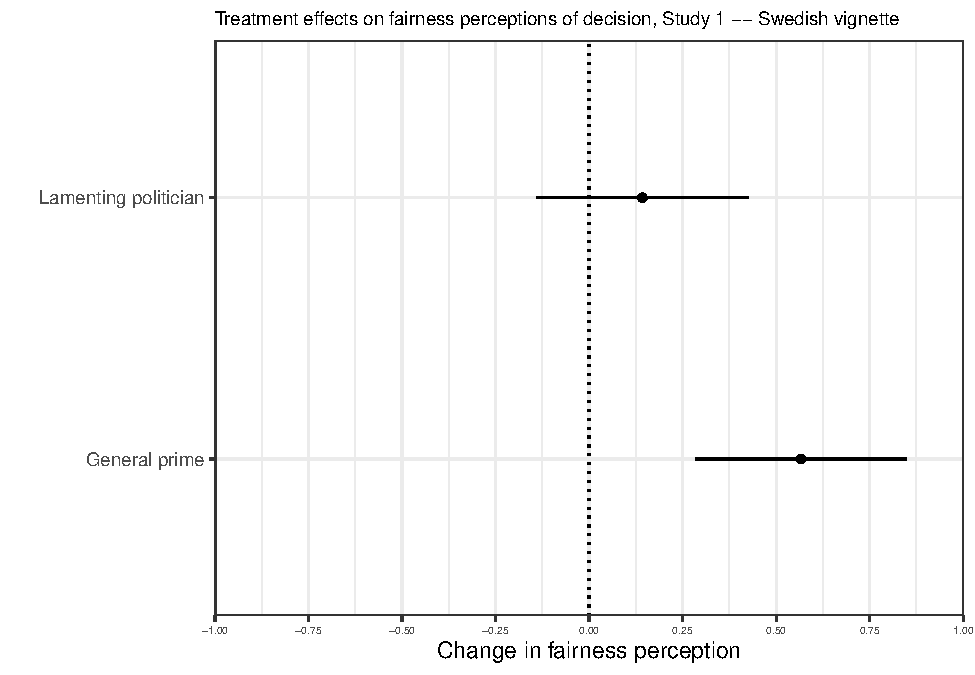
\includegraphics{Goodloser-appendix_files/figure-latex/104_post_fairness-1.pdf} \textbackslash begin\{table\}

\textbackslash caption\{(\#tab:104\_post\_fairness)Treatment effects on fairness perceptions of decision, Study 1 -- Swedish vignette\}
\centering

\begin{tabular}[t]{lrrrr}
\toprule
Treatment value & Estimate & Std. Error & t-statistic & p value\\
\midrule
Not shown & 4.11 & 0.10 & 40.47 & 0.00\\
Lamenting politician & 0.14 & 0.14 & 1.01 & 0.31\\
General prime & 0.57 & 0.14 & 4.00 & 0.00\\
\bottomrule
\end{tabular}

\textbackslash end\{table\}
\#\# Justice
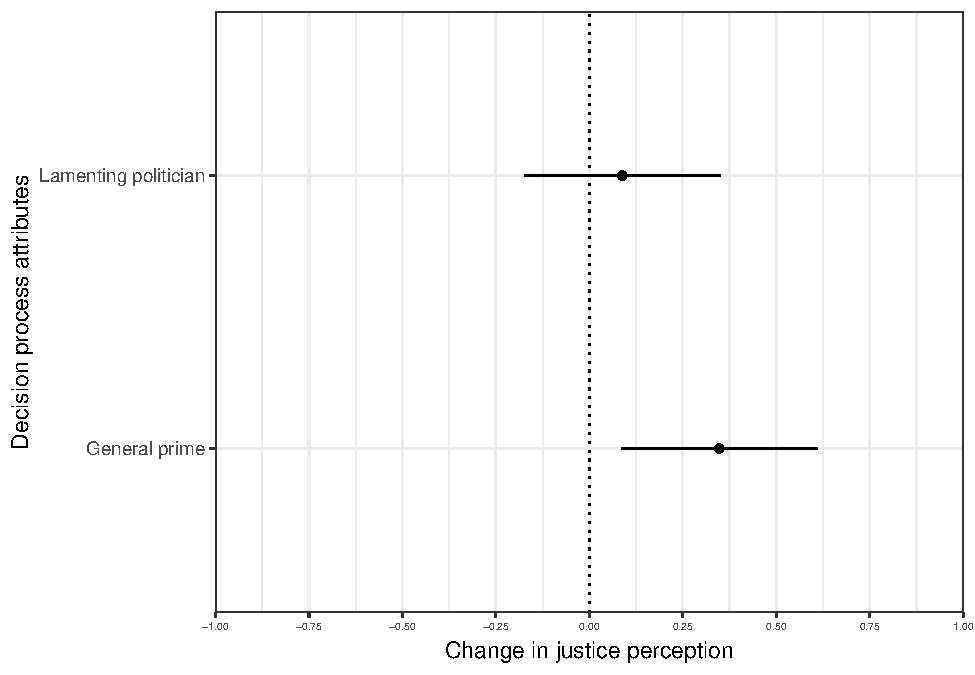
\includegraphics{Goodloser-appendix_files/figure-latex/104_post_justice-1.pdf} \textbackslash begin\{table\}

\textbackslash caption\{(\#tab:104\_post\_justice)Treatment effects on justice perceptions of decision, Study 1 -- Swedish vignette\}
\centering

\begin{tabular}[t]{lrrrr}
\toprule
Treatment value & Estimate & Std. Error & t-statistic & p value\\
\midrule
Not shown & 4.06 & 0.09 & 43.05 & 0.00\\
Lamenting politician & 0.09 & 0.13 & 0.67 & 0.50\\
General prime & 0.35 & 0.13 & 2.65 & 0.01\\
\bottomrule
\end{tabular}

\textbackslash end\{table\}

\hypertarget{decision-evaluation}{%
\section{Decision evaluation}\label{decision-evaluation}}

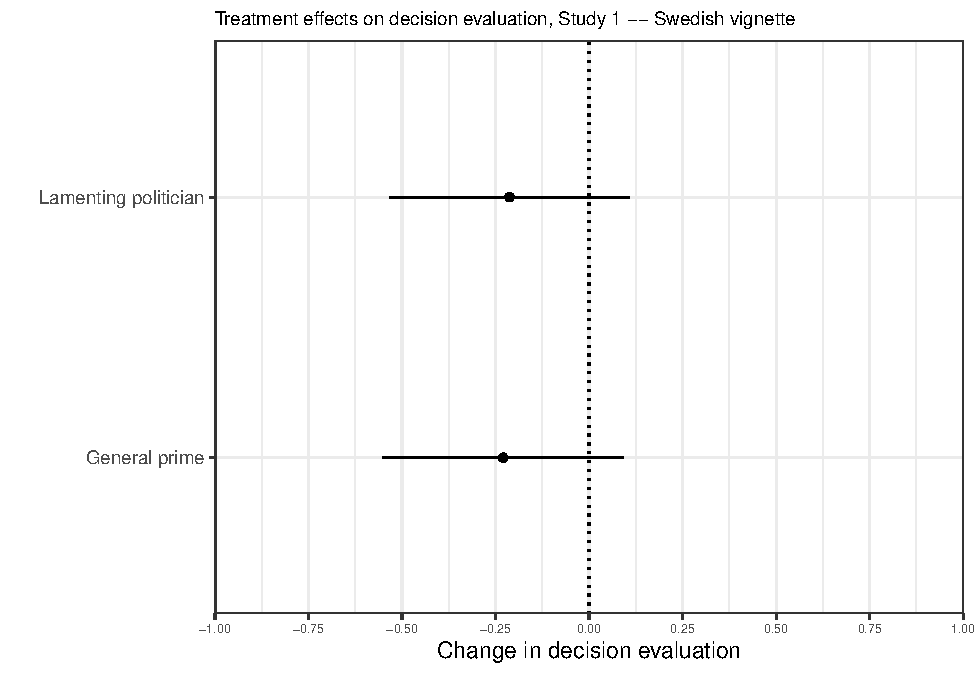
\includegraphics{Goodloser-appendix_files/figure-latex/104_post_eval-1.pdf} \textbackslash begin\{table\}

\textbackslash caption\{(\#tab:104\_post\_eval)Treatment effects on decision evaluation, Study 1 -- Swedish vignette\}
\centering

\begin{tabular}[t]{lrrrr}
\toprule
Treatment value & Estimate & Std. Error & t-statistic & p value\\
\midrule
Not shown & 4.31 & 0.12 & 37.30 & 0.00\\
Lamenting politician & -0.21 & 0.16 & -1.32 & 0.19\\
General prime & -0.23 & 0.16 & -1.43 & 0.15\\
\bottomrule
\end{tabular}

\textbackslash end\{table\}

\hypertarget{willingness-to-accept}{%
\section{Willingness to accept}\label{willingness-to-accept}}

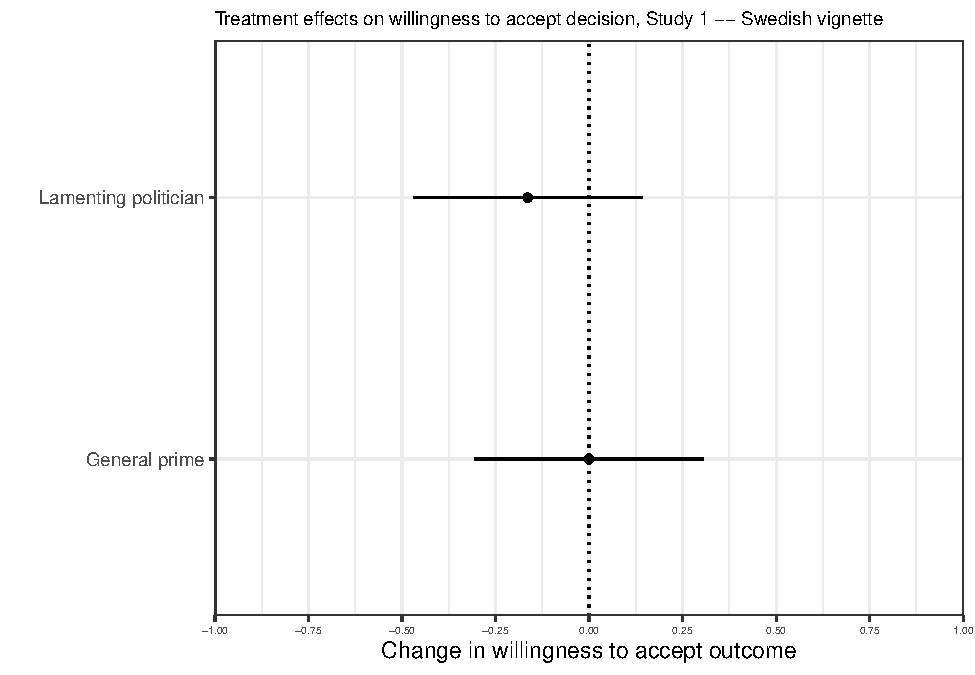
\includegraphics{Goodloser-appendix_files/figure-latex/104_post_accept-1.pdf} \textbackslash begin\{table\}

\textbackslash caption\{(\#tab:104\_post\_accept)Treatment effects on willingness to accept decision, Study 1 -- Swedish vignette\}
\centering

\begin{tabular}[t]{lrrrr}
\toprule
Treatment value & Estimate & Std. Error & t-statistic & p value\\
\midrule
Not shown & 5.18 & 0.11 & 47.02 & 0.00\\
Lamenting politician & -0.16 & 0.15 & -1.07 & 0.28\\
General prime & 0.00 & 0.15 & 0.00 & 1.00\\
\bottomrule
\end{tabular}

\textbackslash end\{table\}

\hypertarget{compliance}{%
\section{Compliance}\label{compliance}}

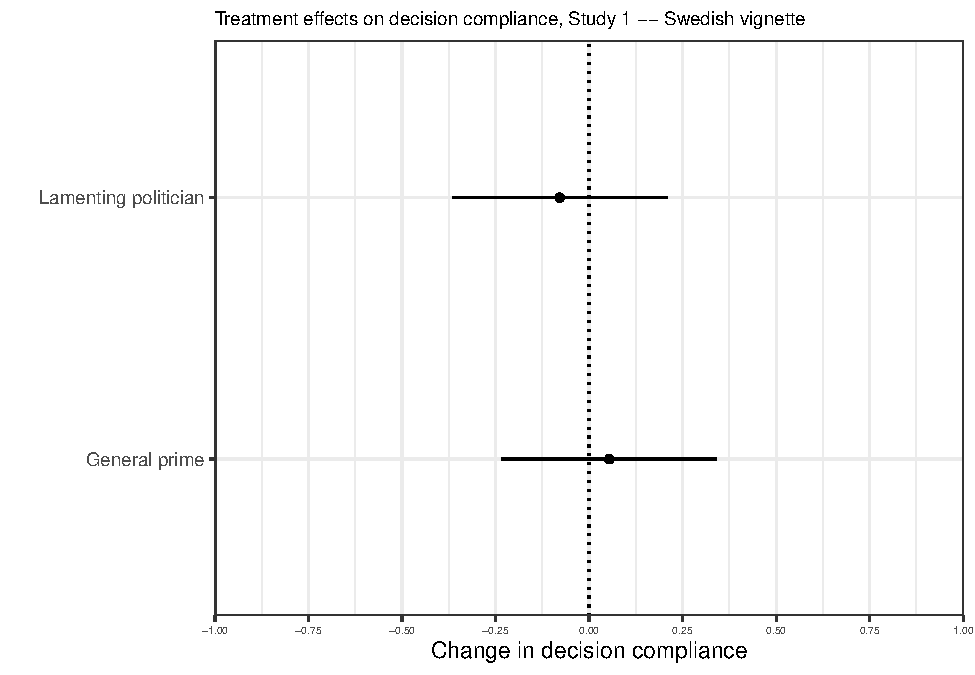
\includegraphics{Goodloser-appendix_files/figure-latex/104_post_comply-1.pdf} \textbackslash begin\{table\}

\textbackslash caption\{(\#tab:104\_post\_comply)Treatment effects on decision compliance, Study 1 -- Swedish vignette\}
\centering

\begin{tabular}[t]{lrrrr}
\toprule
Treatment value & Estimate & Std. Error & t-statistic & p value\\
\midrule
Not shown & 5.14 & 0.10 & 49.88 & 0.00\\
Lamenting politician & -0.08 & 0.14 & -0.55 & 0.59\\
General prime & 0.05 & 0.14 & 0.38 & 0.71\\
\bottomrule
\end{tabular}

\textbackslash end\{table\}

\hypertarget{moderating-effects-of-issue-importance-on-losers}{%
\chapter{Moderating effects of issue importance on losers}\label{moderating-effects-of-issue-importance-on-losers}}

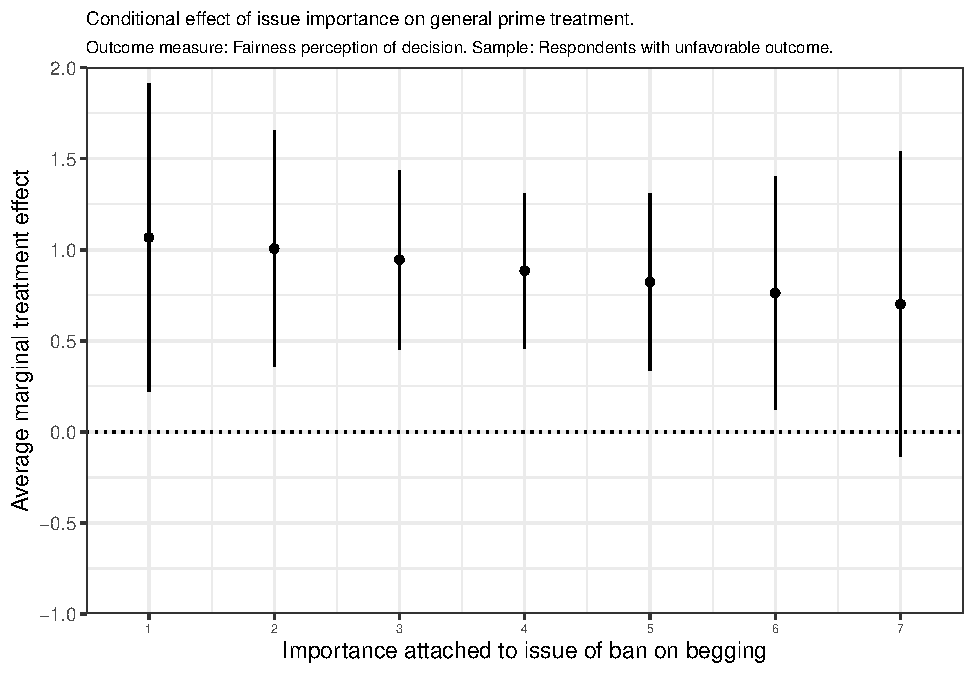
\includegraphics{Goodloser-appendix_files/figure-latex/1045_importance_treatment_fairness-1.pdf} 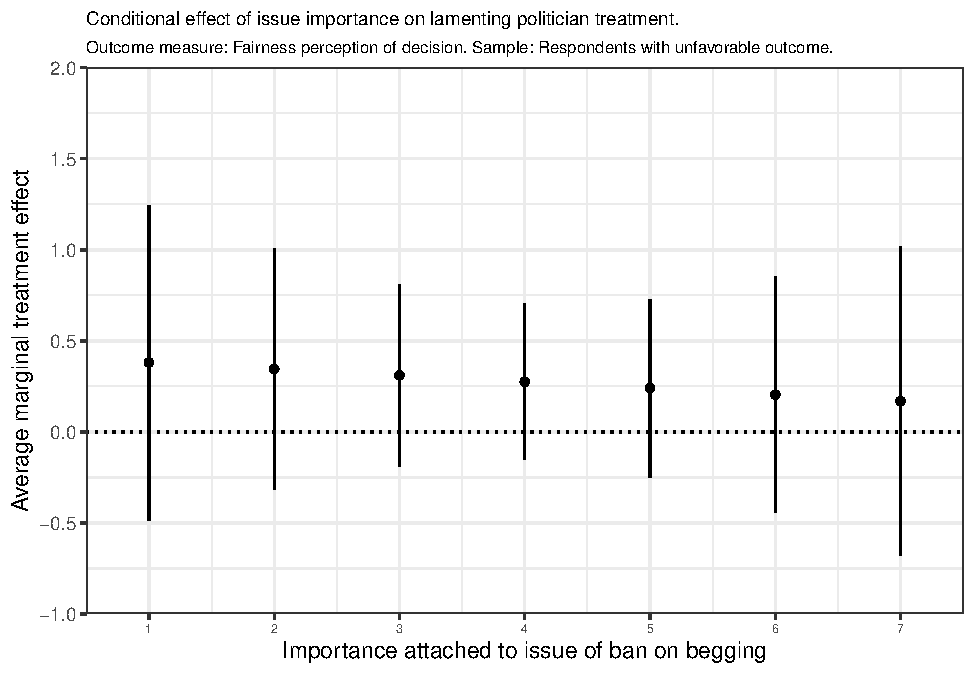
\includegraphics{Goodloser-appendix_files/figure-latex/1045_importance_treatment_fairness-2.pdf} \textbackslash begin\{table\}{[}H{]}

\textbackslash caption\{(\#tab:1045\_importance\_treatment\_fairness)Moderating effects of issue importance on experimental treatment, Study 1 -- Swedish vignette\}
\centering

\begin{tabular}[t]{lrrrrrrr}
\toprule
Factor & Issue importance & AME & SE & z-statistic & p value & Lower & Upper\\
\midrule
General prime & 1 & 1.07 & 0.42 & 2.52 & 0.01 & 0.24 & 1.90\\
General prime & 2 & 1.01 & 0.32 & 3.10 & 0.00 & 0.37 & 1.64\\
General prime & 3 & 0.95 & 0.25 & 3.85 & 0.00 & 0.46 & 1.43\\
General prime & 4 & 0.89 & 0.21 & 4.17 & 0.00 & 0.47 & 1.30\\
General prime & 5 & 0.82 & 0.24 & 3.39 & 0.00 & 0.35 & 1.30\\
\addlinespace
General prime & 6 & 0.76 & 0.32 & 2.38 & 0.02 & 0.13 & 1.39\\
General prime & 7 & 0.70 & 0.42 & 1.67 & 0.09 & -0.12 & 1.52\\
Lamenting politician & 1 & 0.38 & 0.43 & 0.88 & 0.38 & -0.47 & 1.23\\
Lamenting politician & 2 & 0.35 & 0.33 & 1.05 & 0.30 & -0.30 & 0.99\\
Lamenting politician & 3 & 0.31 & 0.25 & 1.24 & 0.21 & -0.18 & 0.80\\
\addlinespace
Lamenting politician & 4 & 0.28 & 0.21 & 1.29 & 0.20 & -0.14 & 0.69\\
Lamenting politician & 5 & 0.24 & 0.25 & 0.98 & 0.33 & -0.24 & 0.72\\
Lamenting politician & 6 & 0.20 & 0.32 & 0.63 & 0.53 & -0.43 & 0.84\\
Lamenting politician & 7 & 0.17 & 0.42 & 0.40 & 0.69 & -0.66 & 1.00\\
\bottomrule
\multicolumn{8}{l}{\textit{Note: }}\\
\multicolumn{8}{l}{Sample: Respondents with unfavorable outcome.}\\
\end{tabular}

\textbackslash end\{table\}

\textbackslash begin\{table\}{[}H{]}

\textbackslash caption\{(\#tab:1045\_exp1\_mods)Moderating effects of issue importance, Study 1 -- Swedish vignette\}
\centering

\begin{tabular}[t]{lrrrr}
\toprule
Treatment value & Estimate & Std. Error & t-statistic & p value\\
\midrule
Intercept & 3.42 & 0.25 & 13.73 & 0.00\\
Lamenting politician & 0.03 & 0.34 & 0.10 & 0.92\\
General prime & 0.81 & 0.34 & 2.41 & 0.02\\
Issue not important to respondent & 0.07 & 0.32 & 0.21 & 0.83\\
Lamenting politician w/ issue not important to respondent & 0.40 & 0.44 & 0.91 & 0.37\\
\addlinespace
General prime w/ issue not important to respondent & 0.12 & 0.43 & 0.29 & 0.78\\
\bottomrule
\multicolumn{5}{l}{\textit{Note: }}\\
\multicolumn{5}{l}{Sample: Respondents with unfavorable outcome.}\\
\end{tabular}

\textbackslash end\{table\}

\hypertarget{effects-on-losers}{%
\chapter{Effects on losers}\label{effects-on-losers}}

\hypertarget{fairness-1}{%
\section{Fairness}\label{fairness-1}}

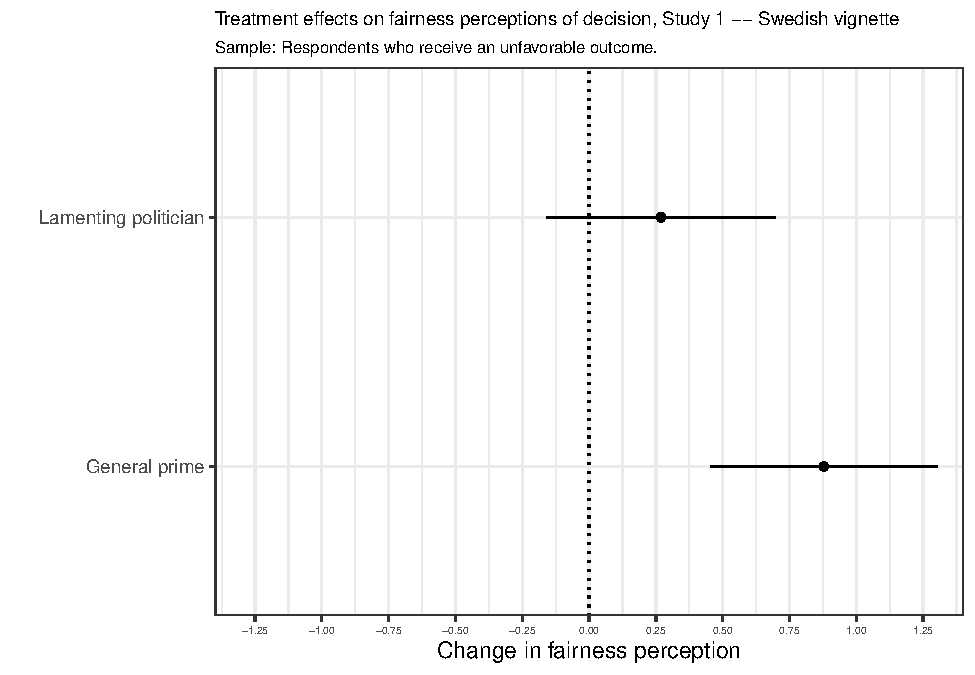
\includegraphics{Goodloser-appendix_files/figure-latex/1055_post_fairness-1.pdf} \textbackslash begin\{table\}

\textbackslash caption\{(\#tab:1055\_post\_fairness)Treatment effects on fairness perceptions of decision, Study 1 -- Swedish vignette\}
\centering

\begin{tabular}[t]{lrrrr}
\toprule
Treatment value & Estimate & Std. Error & t-statistic & p value\\
\midrule
Not shown & 3.46 & 0.16 & 22.32 & 0.00\\
Lamenting politician & 0.27 & 0.21 & 1.26 & 0.21\\
General prime & 0.88 & 0.21 & 4.15 & 0.00\\
\bottomrule
\end{tabular}

\textbackslash end\{table\}

\hypertarget{fairness-ii}{%
\subsection{Fairness II}\label{fairness-ii}}

\begin{quote}
Lamenting politician as reference category
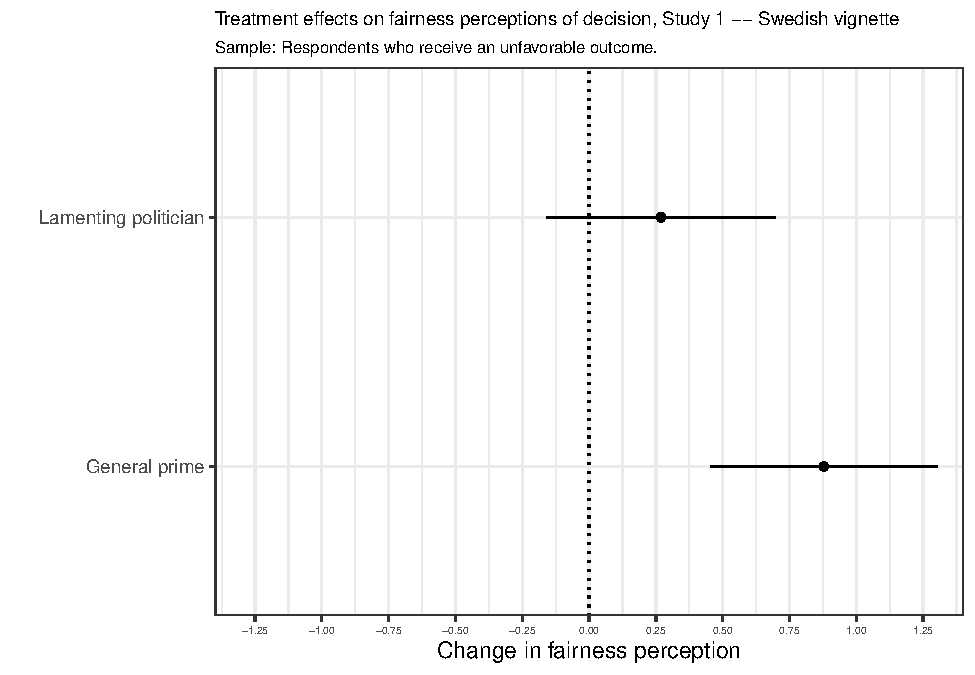
\includegraphics{Goodloser-appendix_files/figure-latex/105_post_fairness-1.pdf} \textbackslash begin\{table\}
\end{quote}

\textbackslash caption\{(\#tab:105\_post\_fairness)Treatment effects on fairness perceptions of decision, Study 1 -- Swedish vignette\}
\centering

\begin{tabular}[t]{lrrrr}
\toprule
Treatment value & Estimate & Std. Error & t-statistic & p value\\
\midrule
Intercept & 3.73 & 0.15 & 25.41 & 0.00\\
Not shown & -0.27 & 0.21 & -1.26 & 0.21\\
General prime & 0.61 & 0.21 & 2.96 & 0.00\\
\bottomrule
\multicolumn{5}{l}{\textit{Note: }}\\
\multicolumn{5}{l}{Lamenting politician set as reference category.}\\
\end{tabular}

\textbackslash end\{table\}

\hypertarget{justice}{%
\section{Justice}\label{justice}}

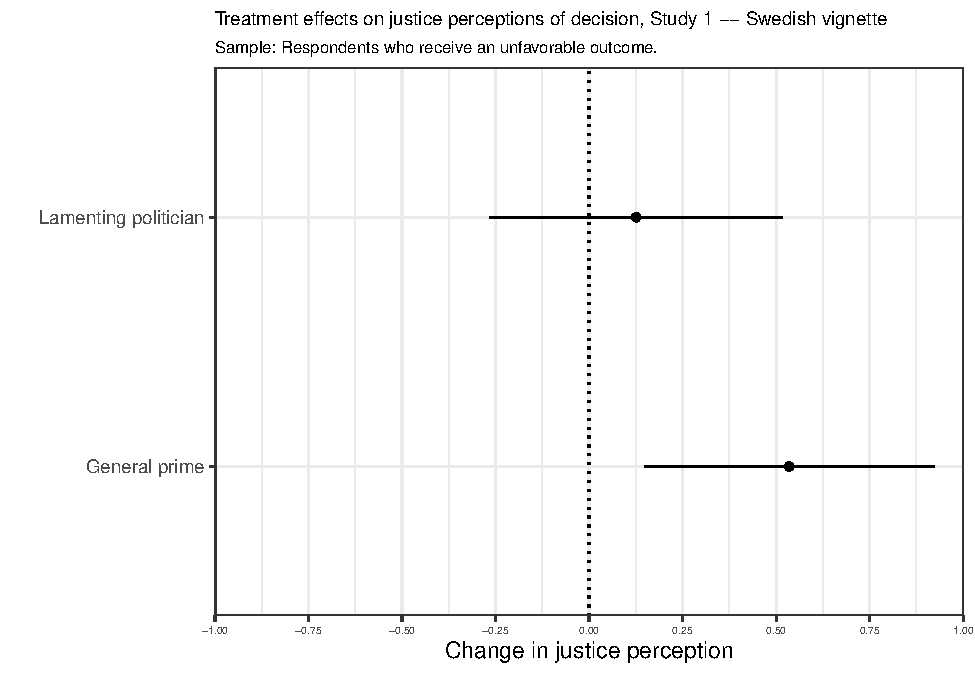
\includegraphics{Goodloser-appendix_files/figure-latex/105_post_justice-1.pdf} \textbackslash begin\{table\}

\textbackslash caption\{(\#tab:105\_post\_justice)Treatment effects on justice perceptions of decision, Study 1 -- Swedish vignette\}
\centering

\begin{tabular}[t]{lrrrr}
\toprule
Treatment value & Estimate & Std. Error & t-statistic & p value\\
\midrule
Not shown & 3.61 & 0.14 & 25.45 & 0.00\\
Lamenting politician & 0.13 & 0.20 & 0.64 & 0.52\\
General prime & 0.53 & 0.19 & 2.76 & 0.01\\
\bottomrule
\end{tabular}

\textbackslash end\{table\}

\hypertarget{decision-evaluation-1}{%
\section{Decision evaluation}\label{decision-evaluation-1}}

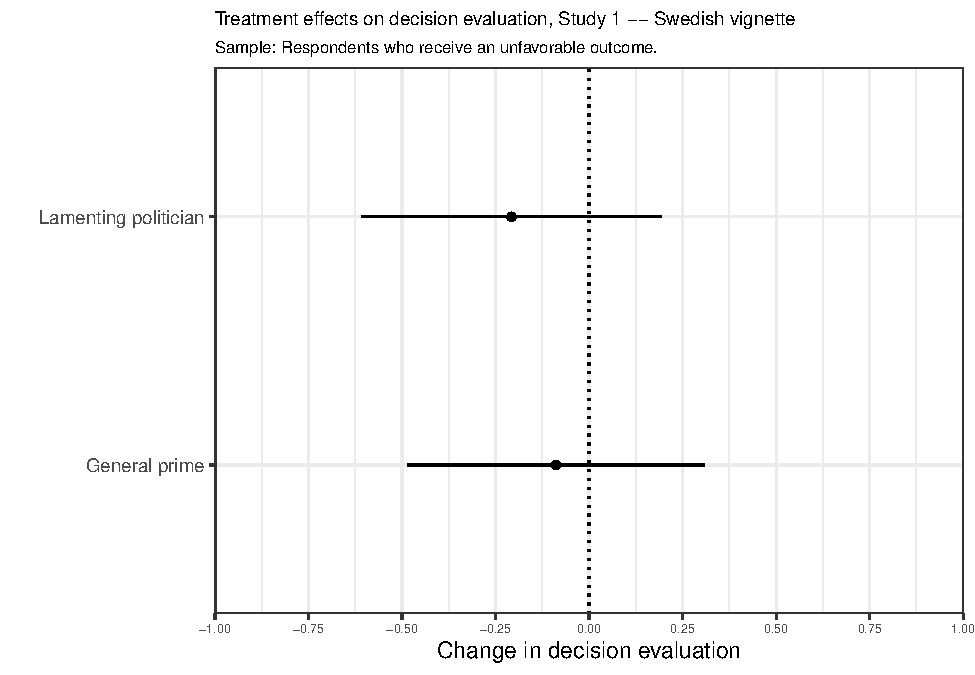
\includegraphics{Goodloser-appendix_files/figure-latex/105_post_eval-1.pdf} \textbackslash begin\{table\}

\textbackslash caption\{(\#tab:105\_post\_eval)Treatment effects on decision evaluation, Study 1 -- Swedish vignette\}
\centering

\begin{tabular}[t]{lrrrr}
\toprule
Treatment value & Estimate & Std. Error & t-statistic & p value\\
\midrule
Not shown & 3.00 & 0.15 & 20.60 & 0.00\\
Lamenting politician & -0.21 & 0.20 & -1.03 & 0.30\\
General prime & -0.09 & 0.20 & -0.44 & 0.66\\
\bottomrule
\end{tabular}

\textbackslash end\{table\}

\hypertarget{willingness-to-accept-1}{%
\section{Willingness to accept}\label{willingness-to-accept-1}}

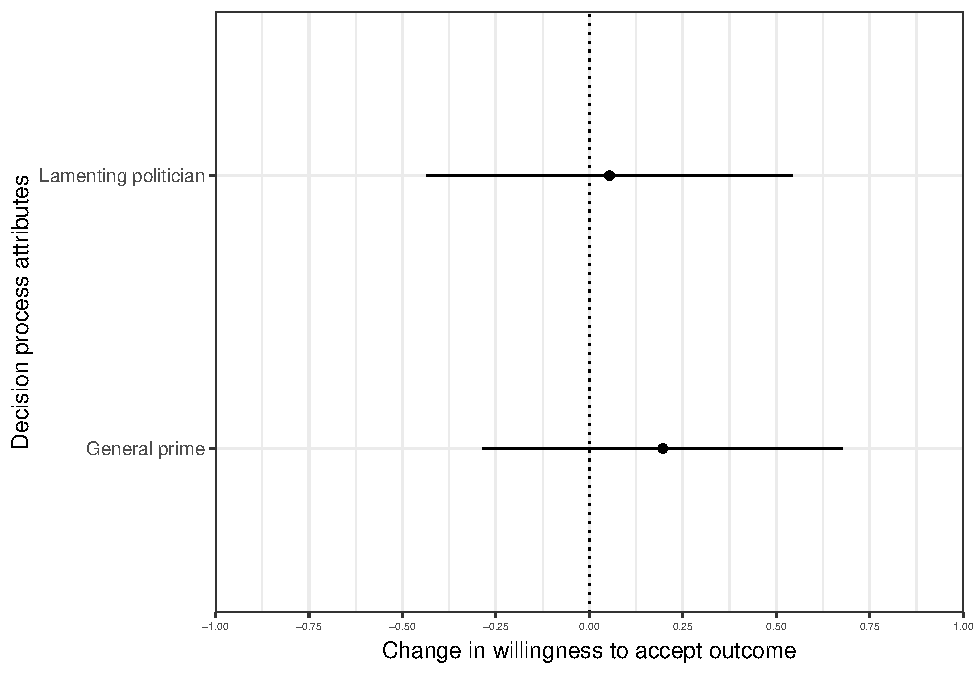
\includegraphics{Goodloser-appendix_files/figure-latex/105_post_accept-1.pdf} \textbackslash begin\{table\}

\textbackslash caption\{(\#tab:105\_post\_accept)Treatment effects on willingness to accept decision, Study 1 -- Swedish vignette\}
\centering

\begin{tabular}[t]{lrrrr}
\toprule
Treatment value & Estimate & Std. Error & t-statistic & p value\\
\midrule
Not shown & 4.31 & 0.17 & 24.95 & 0.00\\
Lamenting politician & -0.22 & 0.24 & -0.93 & 0.35\\
General prime & 0.13 & 0.24 & 0.57 & 0.57\\
\bottomrule
\end{tabular}

\textbackslash end\{table\}

\hypertarget{compliance-1}{%
\section{Compliance}\label{compliance-1}}

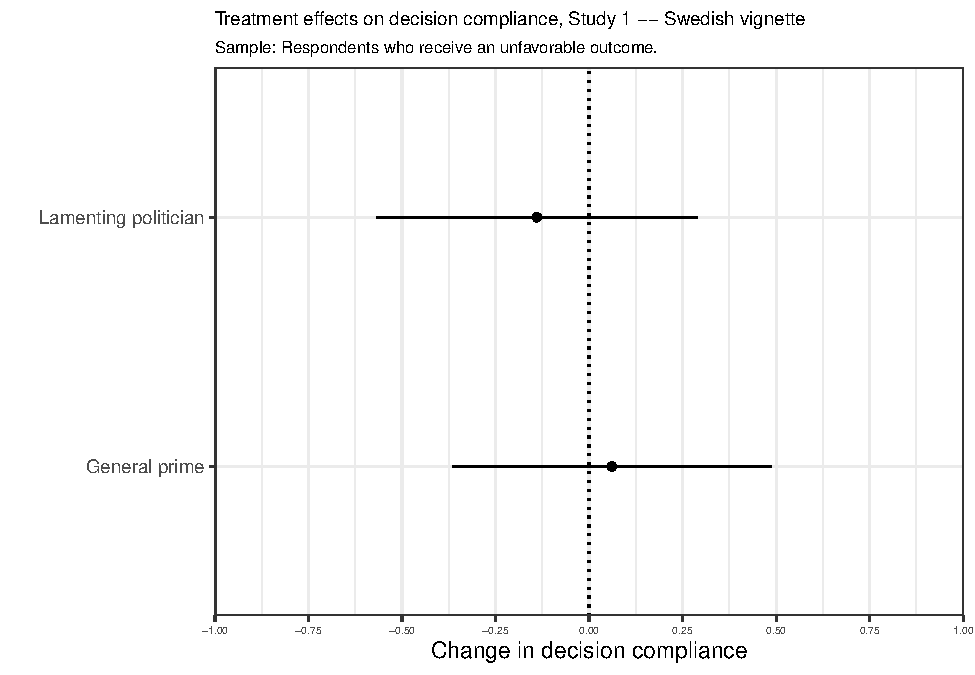
\includegraphics{Goodloser-appendix_files/figure-latex/105_post_comply-1.pdf} \textbackslash begin\{table\}

\textbackslash caption\{(\#tab:105\_post\_comply)Treatment effects on decision compliance, Study 1 -- Swedish vignette\}
\centering

\begin{tabular}[t]{lrrrr}
\toprule
Treatment value & Estimate & Std. Error & t-statistic & p value\\
\midrule
Not shown & 4.46 & 0.16 & 28.58 & 0.00\\
Lamenting politician & -0.14 & 0.22 & -0.65 & 0.52\\
General prime & 0.06 & 0.21 & 0.29 & 0.78\\
\bottomrule
\end{tabular}

\textbackslash end\{table\}

\hypertarget{codebook}{%
\chapter{Codebook}\label{codebook}}

\begin{quote}
This chapter displays the codebook for the data set of the first Good Loser experiment, automatically generated using the R package ``codebook''.
\end{quote}

\begin{verbatim}
## # A tibble: 1,019 x 14
##      Q64     Q63  S3_1_1  S3_2_1 S3_4_1_1 S3_4_1_2  S3_5_1 S3_6_1_1 S3_6_1_2
##    <dbl> <dbl+l> <dbl+l> <dbl+l> <dbl+lb> <dbl+lb> <dbl+l> <dbl+lb> <dbl+lb>
##  1    52 2 [Kvi~ 1 [Jag~ 5 [5]   1 [1 In~       NA 4 [4]   1 [1 My~       NA
##  2    30 2 [Kvi~ 2 [Jag~ 3 [3]   4 [4]          NA 4 [4]   5 [5]          NA
##  3    64 2 [Kvi~ 1 [Jag~ 4 [4]   5 [5]          NA 2 [2]   2 [2]          NA
##  4    43 2 [Kvi~ 2 [Jag~ 2 [2]   4 [4]          NA 4 [4]   7 [7 My~       NA
##  5    74 1 [Man] 2 [Jag~ 7 [7 M~ 4 [4]          NA 4 [4]   4 [4]          NA
##  6    51 2 [Kvi~ 1 [Jag~ 4 [4]   1 [1 In~       NA 1 [1 M~ 4 [4]          NA
##  7    58 1 [Man] 2 [Jag~ 7 [7 M~ 7 [7 My~       NA 7 [7 M~ 6 [6]          NA
##  8    55 1 [Man] 2 [Jag~ 4 [4]   4 [4]          NA 4 [4]   6 [6]          NA
##  9    68 2 [Kvi~ 2 [Jag~ 3 [3]   3 [3]          NA 3 [3]   3 [3]          NA
## 10    32 1 [Man] 2 [Jag~ 5 [5]   6 [6]          NA 6 [6]   5 [5]          NA
## # ... with 1,009 more rows, and 5 more variables: S3_7_1_1 <dbl+lbl>,
## #   S3_7_1_2 <dbl+lbl>, S3_8_1_1 <dbl+lbl>, S3_8_1_2 <dbl+lbl>,
## #   Studie3sel <dbl+lbl>
\end{verbatim}

\hypertarget{metadata}{%
\subsection{Metadata}\label{metadata}}

\hypertarget{description}{%
\subsubsection{Description}\label{description}}

\textbf{Dataset name}: d

The dataset has N=1019 rows and 14 columns.
0 rows have no missing values on any column.

Metadata for search engines

\begin{itemize}
\item
  \textbf{Date published}: 2020-04-06

  \begin{itemize}
  \tightlist
  \item
    \textbf{keywords}: \emph{Q64}, \emph{Q63}, \emph{S3\_1\_1}, \emph{S3\_2\_1}, \emph{S3\_4\_1\_1}, \emph{S3\_4\_1\_2}, \emph{S3\_5\_1}, \emph{S3\_6\_1\_1}, \emph{S3\_6\_1\_2}, \emph{S3\_7\_1\_1}, \emph{S3\_7\_1\_2}, \emph{S3\_8\_1\_1}, \emph{S3\_8\_1\_2} and \emph{Studie3sel}
  \end{itemize}
\end{itemize}

\hypertarget{variables}{%
\section{Variables}\label{variables}}

\hypertarget{Q64}{%
\subsection{Q64}\label{Q64}}

Ålder

\hypertarget{Q64_distribution}{%
\subsubsection{Distribution}\label{Q64_distribution}}

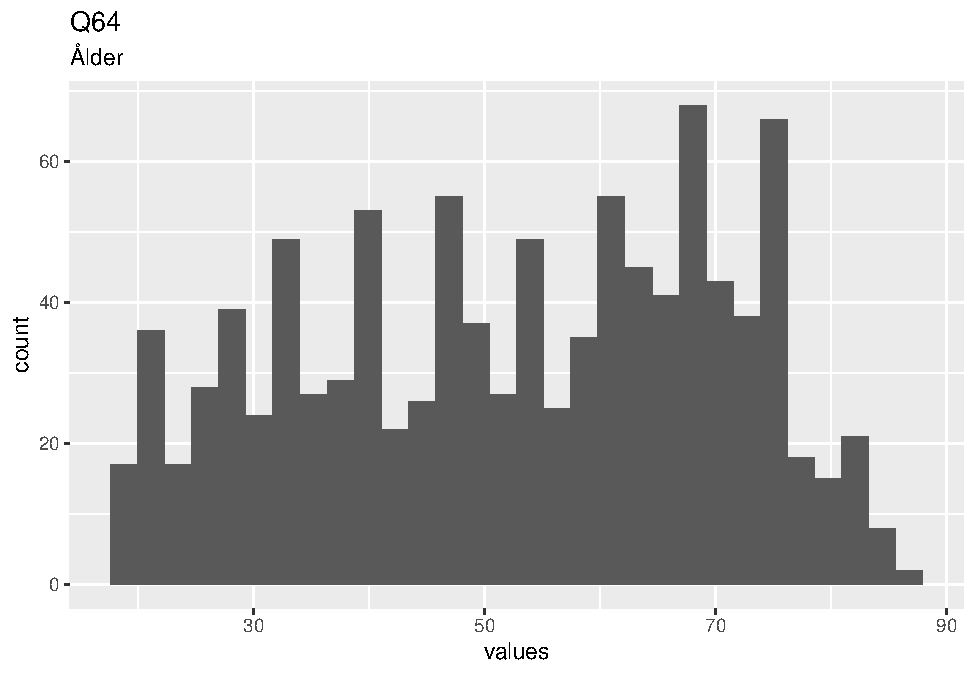
\includegraphics{Goodloser-appendix_files/figure-latex/cb_d_Q64_distribution-1.pdf}

4 missing values.

\hypertarget{Q64_summary}{%
\subsubsection{Summary statistics}\label{Q64_summary}}

\begin{tabular}{l|l|l|r|r|l|l|l|r|r|l|l|l}
\hline
name & label & data_type & n_missing & complete_rate & min & median & max & mean & sd & hist & format.spss & display_width\\
\hline
Q64 & Ålder & numeric & 4 & 0.9961 & 18 & 54 & 86 & 52.46 & 17.74 & ▅▆▆▇▃ & F8.0 & 10\\
\hline
\end{tabular}

\hypertarget{Q63}{%
\subsection{Q63}\label{Q63}}

Kön

\hypertarget{Q63_distribution}{%
\subsubsection{Distribution}\label{Q63_distribution}}

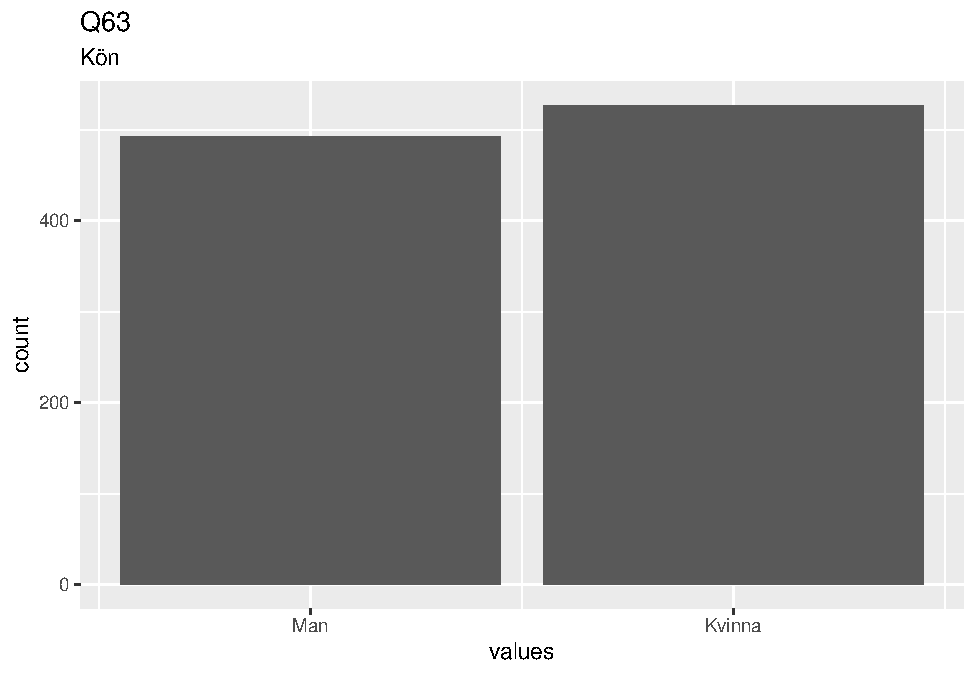
\includegraphics{Goodloser-appendix_files/figure-latex/cb_d_Q63_distribution-1.pdf}

0 missing values.

\hypertarget{Q63_summary}{%
\subsubsection{Summary statistics}\label{Q63_summary}}

\begin{tabular}{l|l|l|l|r|r|l|l|l|r|r|r|l|l|l}
\hline
name & label & data_type & value_labels & n_missing & complete_rate & min & median & max & mean & sd & n_value_labels & hist & format.spss & display_width\\
\hline
Q63 & Kön & haven_labelled & 1. Man,<br>2. Kvinna & 0 & 1 & 1 & 2 & 2 & 1.517 & 0.5 & 2 & ▇▁▁▁▁▁▁▇ & F1.0 & 12\\
\hline
\end{tabular}

\hypertarget{Q63_labels}{%
\subsubsection{Value labels}\label{Q63_labels}}

\begin{itemize}
\tightlist
\item
  \textbf{Man}: \emph{1}
\item
  \textbf{Kvinna}: \emph{2}
\end{itemize}

\hypertarget{S3_1_1}{%
\subsection{S3\_1\_1}\label{S3_1_1}}

I debatten diskuteras ibland att kommunerna skall kunna förbjuda tiggeri inom sina gränser. Vad tycker du själv om att förbjuda tiggeri i kommunen där du bor?

\hypertarget{S3_1_1_distribution}{%
\subsubsection{Distribution}\label{S3_1_1_distribution}}

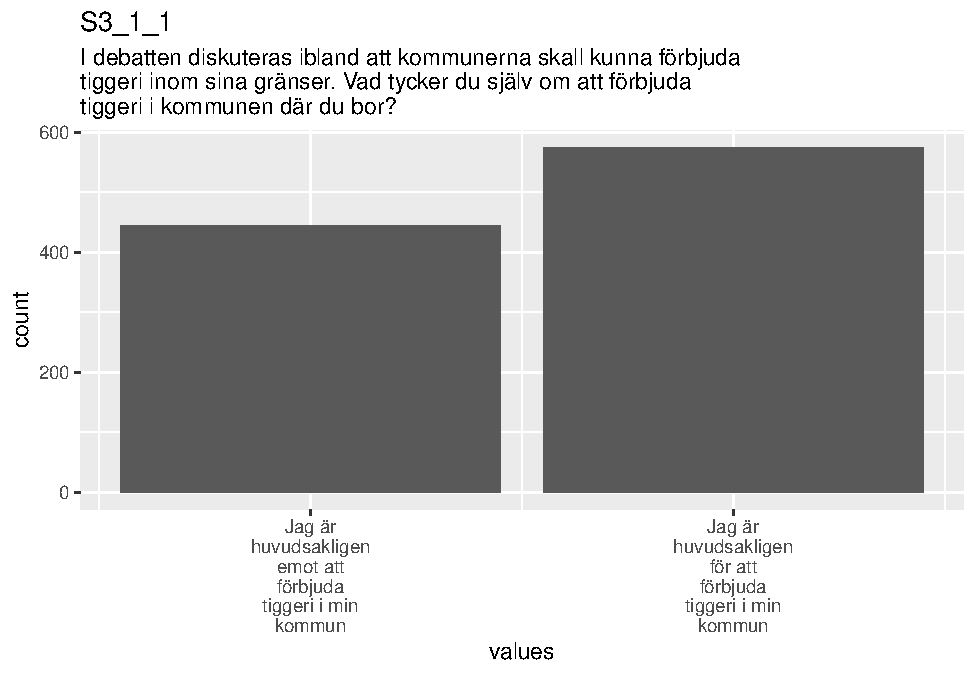
\includegraphics{Goodloser-appendix_files/figure-latex/cb_d_S3_1_1_distribution-1.pdf}

0 missing values.

\hypertarget{S3_1_1_summary}{%
\subsubsection{Summary statistics}\label{S3_1_1_summary}}

\begin{tabular}{l|l|l|l|r|r|l|l|l|r|r|r|l|l|l}
\hline
name & label & data_type & value_labels & n_missing & complete_rate & min & median & max & mean & sd & n_value_labels & hist & format.spss & display_width\\
\hline
S3_1_1 & I debatten diskuteras ibland att kommunerna skall kunna förbjuda tiggeri inom sina gränser. Vad tycker du själv om att förbjuda tiggeri i kommunen där du bor? & haven_labelled & 1. Jag är huvudsakligen emot att förbjuda tiggeri i min kommun,<br>2. Jag är huvudsakligen för att förbjuda tiggeri i min kommun & 0 & 1 & 1 & 2 & 2 & 1.563 & 0.4962 & 2 & ▆▁▁▁▁▁▁▇ & F1.0 & 12\\
\hline
\end{tabular}

\hypertarget{S3_1_1_labels}{%
\subsubsection{Value labels}\label{S3_1_1_labels}}

\begin{itemize}
\tightlist
\item
  \textbf{Jag är huvudsakligen emot att förbjuda tiggeri i min kommun}: \emph{1}
\item
  \textbf{Jag är huvudsakligen för att förbjuda tiggeri i min kommun}: \emph{2}
\end{itemize}

\hypertarget{S3_2_1}{%
\subsection{S3\_2\_1}\label{S3_2_1}}

Hur viktig är frågan för dig personligen?

\hypertarget{S3_2_1_distribution}{%
\subsubsection{Distribution}\label{S3_2_1_distribution}}

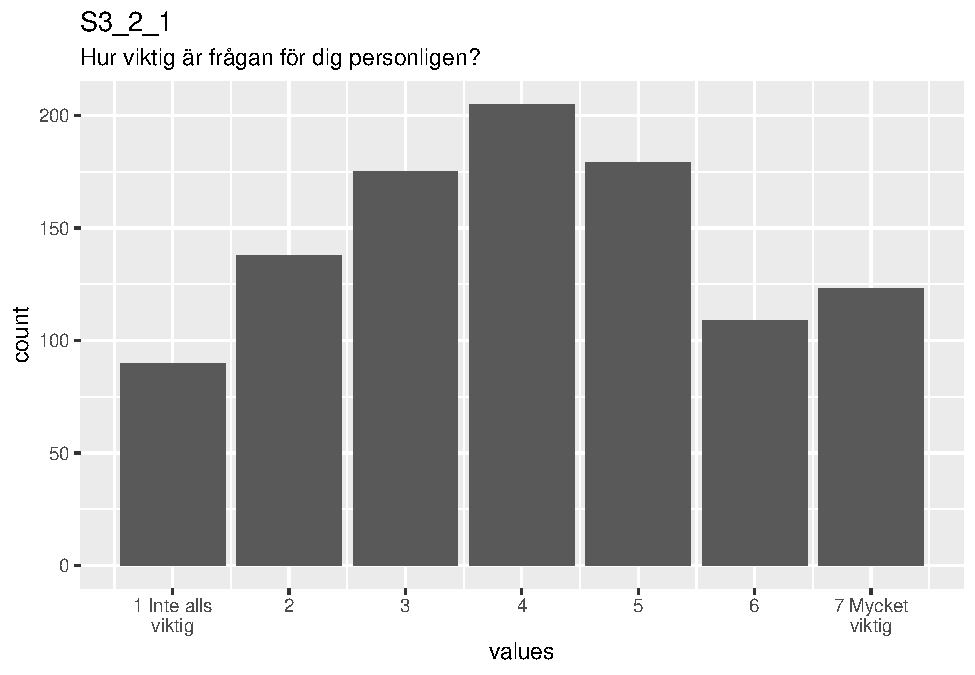
\includegraphics{Goodloser-appendix_files/figure-latex/cb_d_S3_2_1_distribution-1.pdf}

0 missing values.

\hypertarget{S3_2_1_summary}{%
\subsubsection{Summary statistics}\label{S3_2_1_summary}}

\begin{tabular}{l|l|l|l|r|r|l|l|l|r|r|r|l|l|l}
\hline
name & label & data_type & value_labels & n_missing & complete_rate & min & median & max & mean & sd & n_value_labels & hist & format.spss & display_width\\
\hline
S3_2_1 & Hur viktig är frågan för dig personligen? & haven_labelled & 1. 1 Inte alls viktig,<br>2. 2,<br>3. 3,<br>4. 4,<br>5. 5,<br>6. 6,<br>7. 7 Mycket viktig & 0 & 1 & 1 & 4 & 7 & 4.044 & 1.789 & 7 & ▃▆▇▇▁▇▅▅ & F1.0 & 12\\
\hline
\end{tabular}

\hypertarget{S3_2_1_labels}{%
\subsubsection{Value labels}\label{S3_2_1_labels}}

\begin{itemize}
\tightlist
\item
  \textbf{1 Inte alls viktig}: \emph{1}
\item
  \textbf{2}: \emph{2}
\item
  \textbf{3}: \emph{3}
\item
  \textbf{4}: \emph{4}
\item
  \textbf{5}: \emph{5}
\item
  \textbf{6}: \emph{6}
\item
  \textbf{7 Mycket viktig}: \emph{7}
\end{itemize}

\hypertarget{S3_4_1_1}{%
\subsection{S3\_4\_1\_1}\label{S3_4_1_1}}

Hur rättvist tycker du att det gick till när det fattades beslut om att förbjuda tiggeri?

\hypertarget{S3_4_1_1_distribution}{%
\subsubsection{Distribution}\label{S3_4_1_1_distribution}}

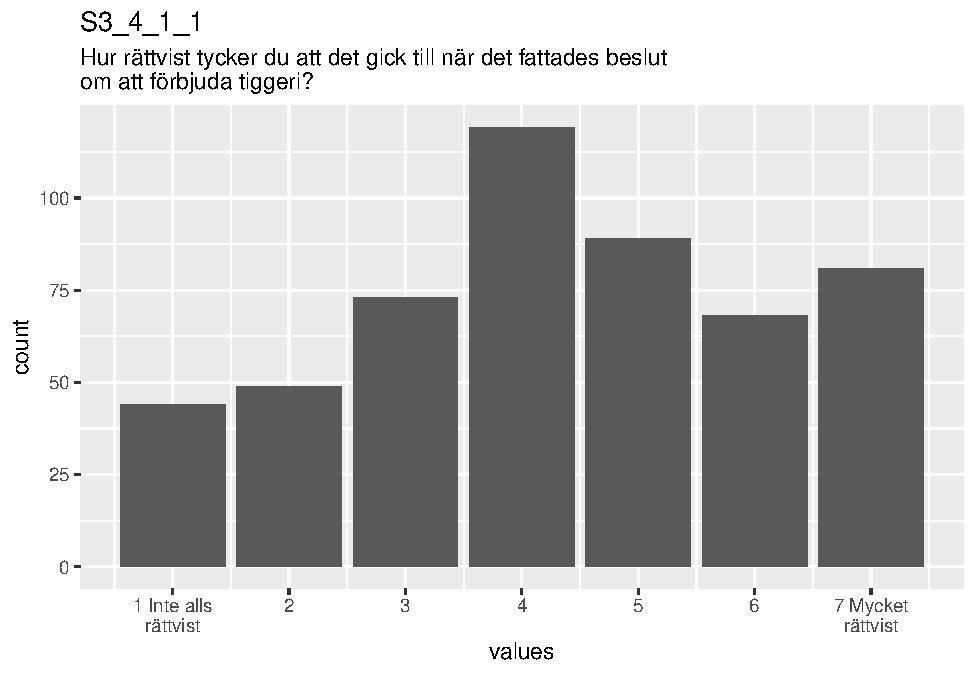
\includegraphics{Goodloser-appendix_files/figure-latex/cb_d_S3_4_1_1_distribution-1.pdf}

496 missing values.

\hypertarget{S3_4_1_1_summary}{%
\subsubsection{Summary statistics}\label{S3_4_1_1_summary}}

\begin{tabular}{l|l|l|l|r|r|l|l|l|r|r|r|l|l|l}
\hline
name & label & data_type & value_labels & n_missing & complete_rate & min & median & max & mean & sd & n_value_labels & hist & format.spss & display_width\\
\hline
S3_4_1_1 & Hur rättvist tycker du att det gick till när det fattades beslut om att förbjuda tiggeri? & haven_labelled & 1. 1 Inte alls rättvist,<br>2. 2,<br>3. 3,<br>4. 4,<br>5. 5,<br>6. 6,<br>7. 7 Mycket rättvist & 496 & 0.5132 & 1 & 4 & 7 & 4.316 & 1.806 & 7 & ▃▃▅▇▁▆▅▆ & F1.0 & 12\\
\hline
\end{tabular}

\hypertarget{S3_4_1_1_labels}{%
\subsubsection{Value labels}\label{S3_4_1_1_labels}}

\begin{itemize}
\tightlist
\item
  \textbf{1 Inte alls rättvist}: \emph{1}
\item
  \textbf{2}: \emph{2}
\item
  \textbf{3}: \emph{3}
\item
  \textbf{4}: \emph{4}
\item
  \textbf{5}: \emph{5}
\item
  \textbf{6}: \emph{6}
\item
  \textbf{7 Mycket rättvist}: \emph{7}
\end{itemize}

\hypertarget{S3_4_1_2}{%
\subsection{S3\_4\_1\_2}\label{S3_4_1_2}}

Hur rättvist tycker du att det gick till när det fattades beslut om att inte förbjuda tiggeri?

\hypertarget{S3_4_1_2_distribution}{%
\subsubsection{Distribution}\label{S3_4_1_2_distribution}}

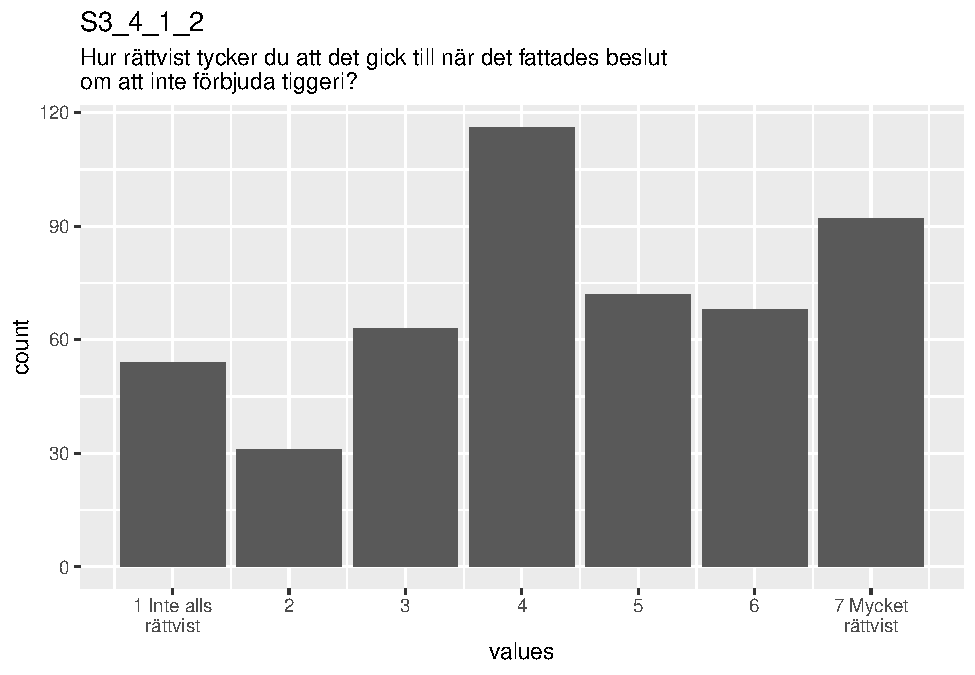
\includegraphics{Goodloser-appendix_files/figure-latex/cb_d_S3_4_1_2_distribution-1.pdf}

523 missing values.

\hypertarget{S3_4_1_2_summary}{%
\subsubsection{Summary statistics}\label{S3_4_1_2_summary}}

\begin{tabular}{l|l|l|l|r|r|l|l|l|r|r|r|l|l}
\hline
name & label & data_type & value_labels & n_missing & complete_rate & min & median & max & mean & sd & n_value_labels & hist & format.spss\\
\hline
S3_4_1_2 & Hur rättvist tycker du att det gick till när det fattades beslut om att inte förbjuda tiggeri? & haven_labelled & 1. 1 Inte alls rättvist,<br>2. 2,<br>3. 3,<br>4. 4,<br>5. 5,<br>6. 6,<br>7. 7 Mycket rättvist & 523 & 0.4868 & 1 & 4 & 7 & 4.397 & 1.889 & 7 & ▃▂▅▇▁▅▅▆ & F1.0\\
\hline
\end{tabular}

\hypertarget{S3_4_1_2_labels}{%
\subsubsection{Value labels}\label{S3_4_1_2_labels}}

\begin{itemize}
\tightlist
\item
  \textbf{1 Inte alls rättvist}: \emph{1}
\item
  \textbf{2}: \emph{2}
\item
  \textbf{3}: \emph{3}
\item
  \textbf{4}: \emph{4}
\item
  \textbf{5}: \emph{5}
\item
  \textbf{6}: \emph{6}
\item
  \textbf{7 Mycket rättvist}: \emph{7}
\end{itemize}

\hypertarget{S3_5_1}{%
\subsection{S3\_5\_1}\label{S3_5_1}}

Och hur schysst tycker du att beslutsproceduren var?

\hypertarget{S3_5_1_distribution}{%
\subsubsection{Distribution}\label{S3_5_1_distribution}}

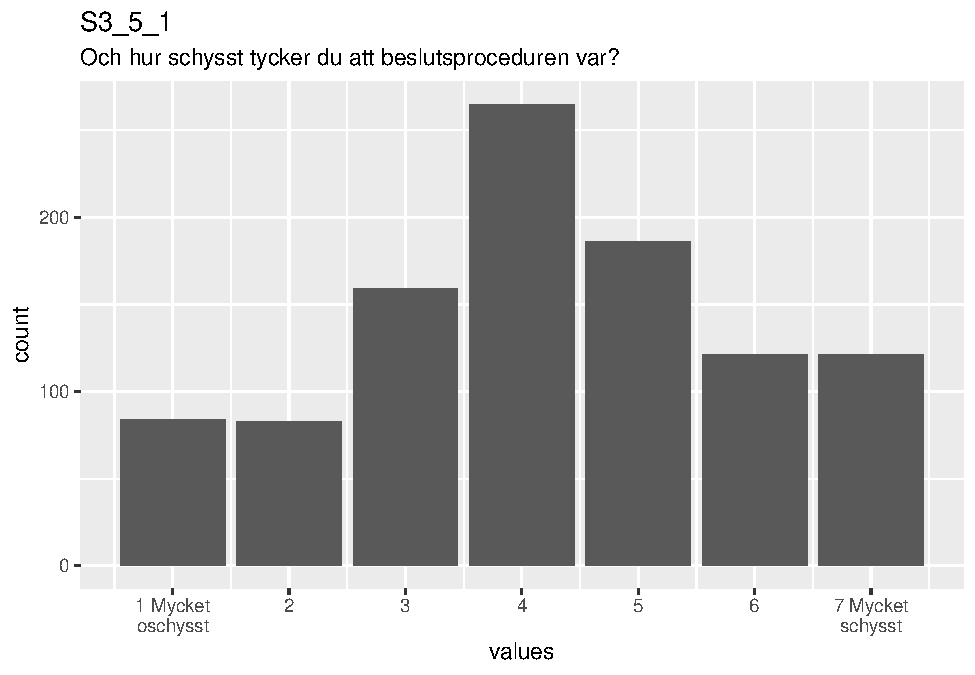
\includegraphics{Goodloser-appendix_files/figure-latex/cb_d_S3_5_1_distribution-1.pdf}

0 missing values.

\hypertarget{S3_5_1_summary}{%
\subsubsection{Summary statistics}\label{S3_5_1_summary}}

\begin{tabular}{l|l|l|l|r|r|l|l|l|r|r|r|l|l|l}
\hline
name & label & data_type & value_labels & n_missing & complete_rate & min & median & max & mean & sd & n_value_labels & hist & format.spss & display_width\\
\hline
S3_5_1 & Och hur schysst tycker du att beslutsproceduren var? & haven_labelled & 1. 1 Mycket oschysst,<br>2. 2,<br>3. 3,<br>4. 4,<br>5. 5,<br>6. 6,<br>7. 7 Mycket schysst & 0 & 1 & 1 & 4 & 7 & 4.21 & 1.706 & 7 & ▂▂▅▇▁▆▃▃ & F1.0 & 12\\
\hline
\end{tabular}

\hypertarget{S3_5_1_labels}{%
\subsubsection{Value labels}\label{S3_5_1_labels}}

\begin{itemize}
\tightlist
\item
  \textbf{1 Mycket oschysst}: \emph{1}
\item
  \textbf{2}: \emph{2}
\item
  \textbf{3}: \emph{3}
\item
  \textbf{4}: \emph{4}
\item
  \textbf{5}: \emph{5}
\item
  \textbf{6}: \emph{6}
\item
  \textbf{7 Mycket schysst}: \emph{7}
\end{itemize}

\hypertarget{S3_6_1_1}{%
\subsection{S3\_6\_1\_1}\label{S3_6_1_1}}

Och om du tänker på själva beslutet att förbjuda tiggeri. Vad tycker Du allmänt sett om beslutet?

\hypertarget{S3_6_1_1_distribution}{%
\subsubsection{Distribution}\label{S3_6_1_1_distribution}}

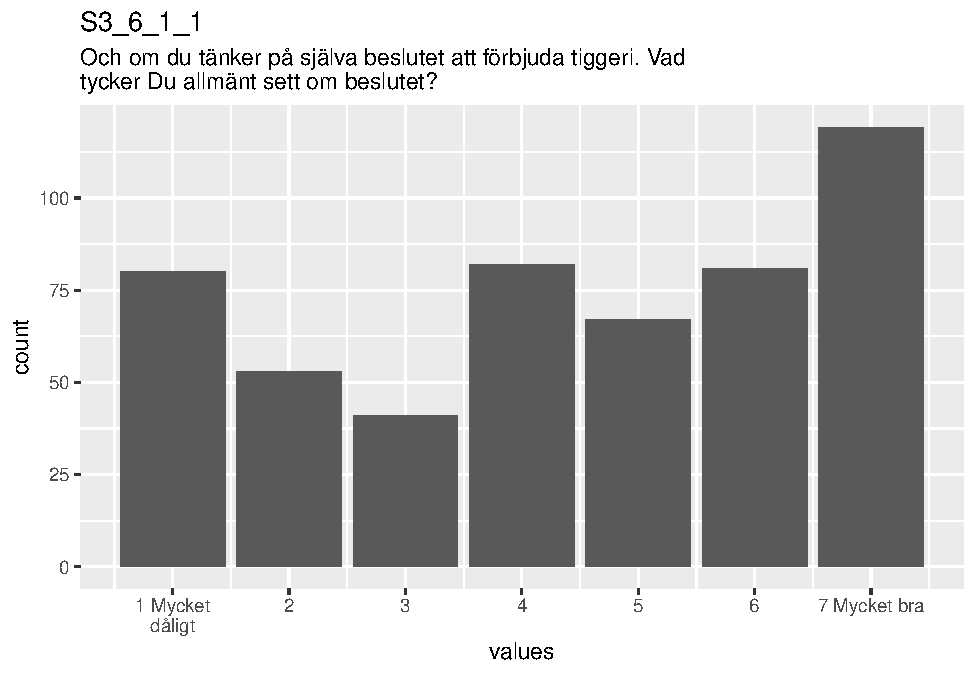
\includegraphics{Goodloser-appendix_files/figure-latex/cb_d_S3_6_1_1_distribution-1.pdf}

496 missing values.

\hypertarget{S3_6_1_1_summary}{%
\subsubsection{Summary statistics}\label{S3_6_1_1_summary}}

\begin{tabular}{l|l|l|l|r|r|l|l|l|r|r|r|l|l|l}
\hline
name & label & data_type & value_labels & n_missing & complete_rate & min & median & max & mean & sd & n_value_labels & hist & format.spss & display_width\\
\hline
S3_6_1_1 & Och om du tänker på själva beslutet att förbjuda tiggeri. Vad tycker Du allmänt sett om beslutet? & haven_labelled & 1. 1 Mycket dåligt,<br>2. 2,<br>3. 3,<br>4. 4,<br>5. 5,<br>6. 6,<br>7. 7 Mycket bra & 496 & 0.5132 & 1 & 5 & 7 & 4.38 & 2.126 & 7 & ▆▃▃▆▁▅▆▇ & F1.0 & 12\\
\hline
\end{tabular}

\hypertarget{S3_6_1_1_labels}{%
\subsubsection{Value labels}\label{S3_6_1_1_labels}}

\begin{itemize}
\tightlist
\item
  \textbf{1 Mycket dåligt}: \emph{1}
\item
  \textbf{2}: \emph{2}
\item
  \textbf{3}: \emph{3}
\item
  \textbf{4}: \emph{4}
\item
  \textbf{5}: \emph{5}
\item
  \textbf{6}: \emph{6}
\item
  \textbf{7 Mycket bra}: \emph{7}
\end{itemize}

\hypertarget{S3_6_1_2}{%
\subsection{S3\_6\_1\_2}\label{S3_6_1_2}}

Och om du tänker på själva beslutet att inte förbjuda tiggeri. Vad tycker Du allmänt sett om beslutet?

\hypertarget{S3_6_1_2_distribution}{%
\subsubsection{Distribution}\label{S3_6_1_2_distribution}}

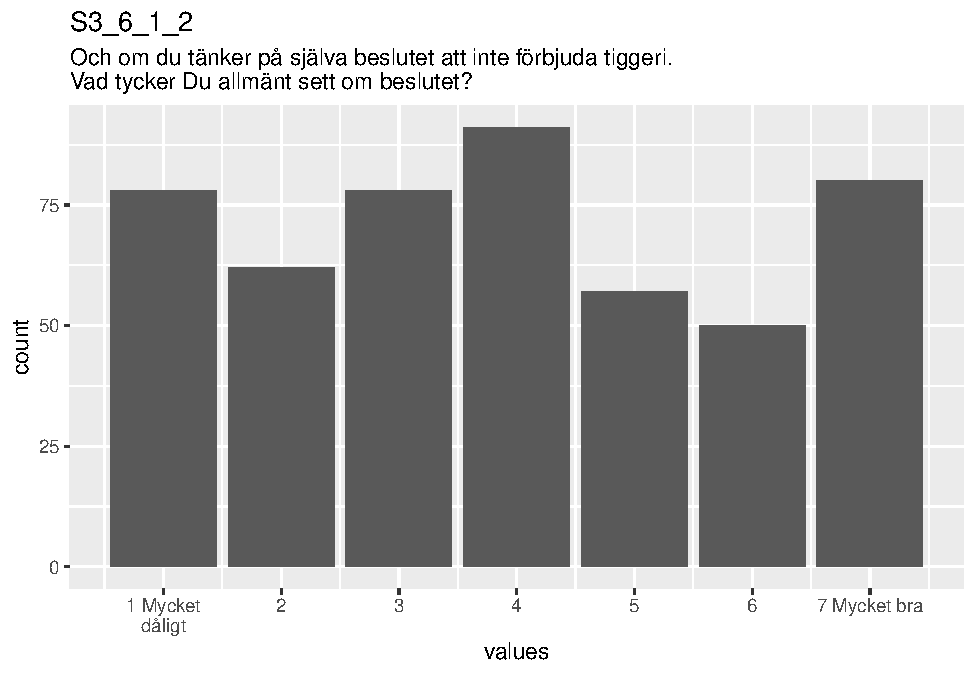
\includegraphics{Goodloser-appendix_files/figure-latex/cb_d_S3_6_1_2_distribution-1.pdf}

523 missing values.

\hypertarget{S3_6_1_2_summary}{%
\subsubsection{Summary statistics}\label{S3_6_1_2_summary}}

\begin{tabular}{l|l|l|l|r|r|l|l|l|r|r|r|l|l}
\hline
name & label & data_type & value_labels & n_missing & complete_rate & min & median & max & mean & sd & n_value_labels & hist & format.spss\\
\hline
S3_6_1_2 & Och om du tänker på själva beslutet att inte förbjuda tiggeri. Vad tycker Du allmänt sett om beslutet? & haven_labelled & 1. 1 Mycket dåligt,<br>2. 2,<br>3. 3,<br>4. 4,<br>5. 5,<br>6. 6,<br>7. 7 Mycket bra & 523 & 0.4868 & 1 & 4 & 7 & 3.921 & 2.011 & 7 & ▇▆▇▇▁▅▅▇ & F1.0\\
\hline
\end{tabular}

\hypertarget{S3_6_1_2_labels}{%
\subsubsection{Value labels}\label{S3_6_1_2_labels}}

\begin{itemize}
\tightlist
\item
  \textbf{1 Mycket dåligt}: \emph{1}
\item
  \textbf{2}: \emph{2}
\item
  \textbf{3}: \emph{3}
\item
  \textbf{4}: \emph{4}
\item
  \textbf{5}: \emph{5}
\item
  \textbf{6}: \emph{6}
\item
  \textbf{7 Mycket bra}: \emph{7}
\end{itemize}

\hypertarget{S3_7_1_1}{%
\subsection{S3\_7\_1\_1}\label{S3_7_1_1}}

Hur villig är du att acceptera och följa beslutet att förbjuda tiggeri?

\hypertarget{S3_7_1_1_distribution}{%
\subsubsection{Distribution}\label{S3_7_1_1_distribution}}

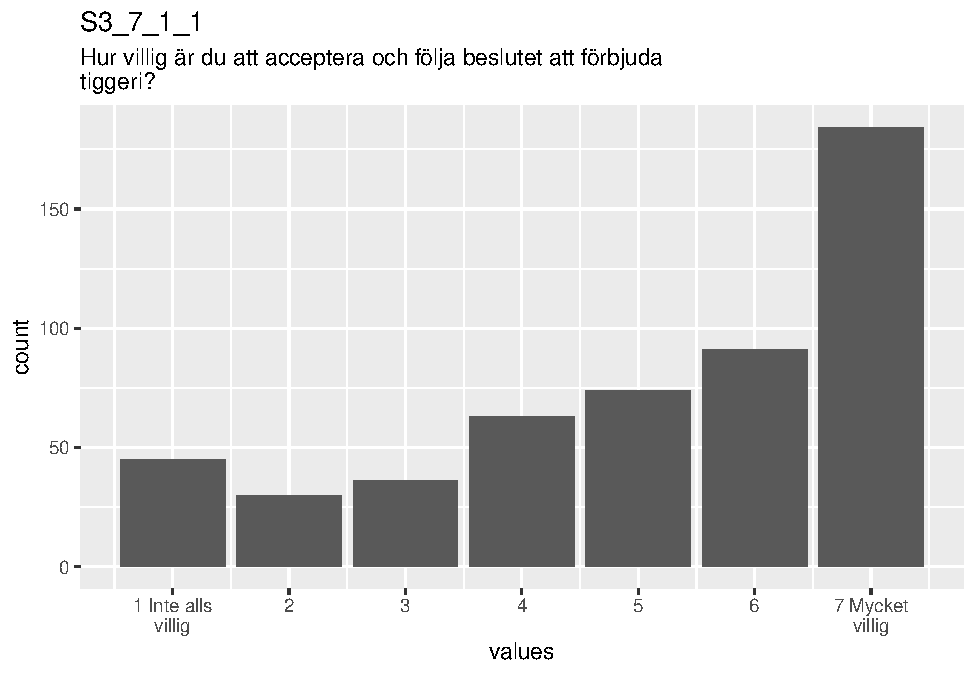
\includegraphics{Goodloser-appendix_files/figure-latex/cb_d_S3_7_1_1_distribution-1.pdf}

496 missing values.

\hypertarget{S3_7_1_1_summary}{%
\subsubsection{Summary statistics}\label{S3_7_1_1_summary}}

\begin{tabular}{l|l|l|l|r|r|l|l|l|r|r|r|l|l|l}
\hline
name & label & data_type & value_labels & n_missing & complete_rate & min & median & max & mean & sd & n_value_labels & hist & format.spss & display_width\\
\hline
S3_7_1_1 & Hur villig är du att acceptera och följa beslutet att förbjuda tiggeri? & haven_labelled & 1. 1 Inte alls villig,<br>2. 2,<br>3. 3,<br>4. 4,<br>5. 5,<br>6. 6,<br>7. 7 Mycket villig & 496 & 0.5132 & 1 & 6 & 7 & 5.103 & 1.966 & 7 & ▂▁▂▃▁▃▃▇ & F1.0 & 12\\
\hline
\end{tabular}

\hypertarget{S3_7_1_1_labels}{%
\subsubsection{Value labels}\label{S3_7_1_1_labels}}

\begin{itemize}
\tightlist
\item
  \textbf{1 Inte alls villig}: \emph{1}
\item
  \textbf{2}: \emph{2}
\item
  \textbf{3}: \emph{3}
\item
  \textbf{4}: \emph{4}
\item
  \textbf{5}: \emph{5}
\item
  \textbf{6}: \emph{6}
\item
  \textbf{7 Mycket villig}: \emph{7}
\end{itemize}

\hypertarget{S3_7_1_2}{%
\subsection{S3\_7\_1\_2}\label{S3_7_1_2}}

Hur villig är du att acceptera och följa beslutet att inte förbjuda tiggeri?

\hypertarget{S3_7_1_2_distribution}{%
\subsubsection{Distribution}\label{S3_7_1_2_distribution}}

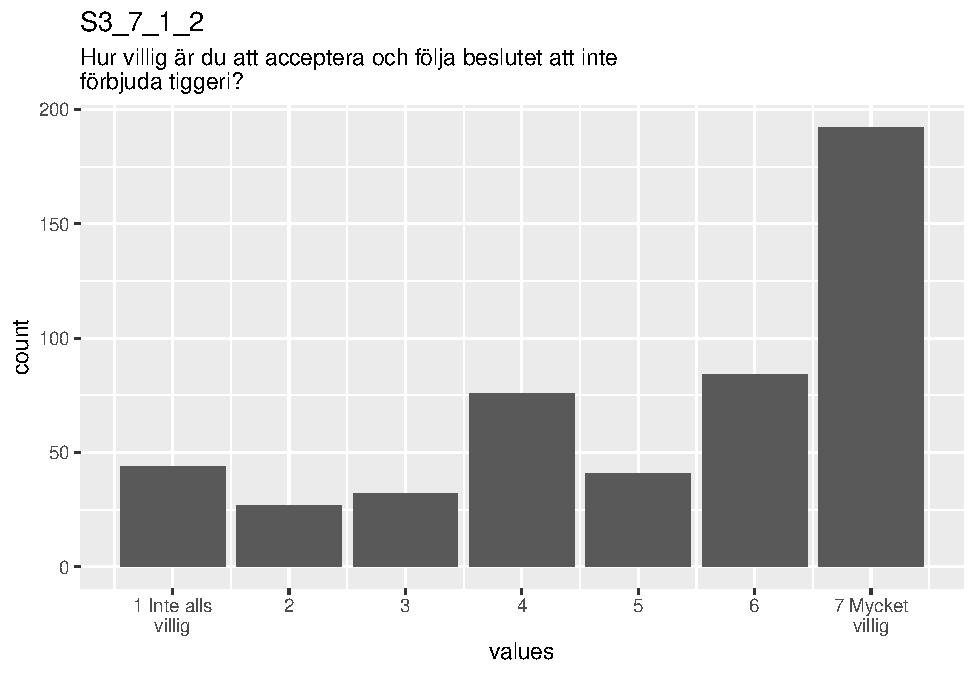
\includegraphics{Goodloser-appendix_files/figure-latex/cb_d_S3_7_1_2_distribution-1.pdf}

523 missing values.

\hypertarget{S3_7_1_2_summary}{%
\subsubsection{Summary statistics}\label{S3_7_1_2_summary}}

\begin{tabular}{l|l|l|l|r|r|l|l|l|r|r|r|l|l}
\hline
name & label & data_type & value_labels & n_missing & complete_rate & min & median & max & mean & sd & n_value_labels & hist & format.spss\\
\hline
S3_7_1_2 & Hur villig är du att acceptera och följa beslutet att inte förbjuda tiggeri? & haven_labelled & 1. 1 Inte alls villig,<br>2. 2,<br>3. 3,<br>4. 4,<br>5. 5,<br>6. 6,<br>7. 7 Mycket villig & 523 & 0.4868 & 1 & 6 & 7 & 5.143 & 2.006 & 7 & ▂▁▁▃▁▂▃▇ & F1.0\\
\hline
\end{tabular}

\hypertarget{S3_7_1_2_labels}{%
\subsubsection{Value labels}\label{S3_7_1_2_labels}}

\begin{itemize}
\tightlist
\item
  \textbf{1 Inte alls villig}: \emph{1}
\item
  \textbf{2}: \emph{2}
\item
  \textbf{3}: \emph{3}
\item
  \textbf{4}: \emph{4}
\item
  \textbf{5}: \emph{5}
\item
  \textbf{6}: \emph{6}
\item
  \textbf{7 Mycket villig}: \emph{7}
\end{itemize}

\hypertarget{S3_8_1_1}{%
\subsection{S3\_8\_1\_1}\label{S3_8_1_1}}

När det gäller att följa eller motarbeta beslutet att förbjuda tiggeri, var på skalan skulle du placera dig?

\hypertarget{S3_8_1_1_distribution}{%
\subsubsection{Distribution}\label{S3_8_1_1_distribution}}

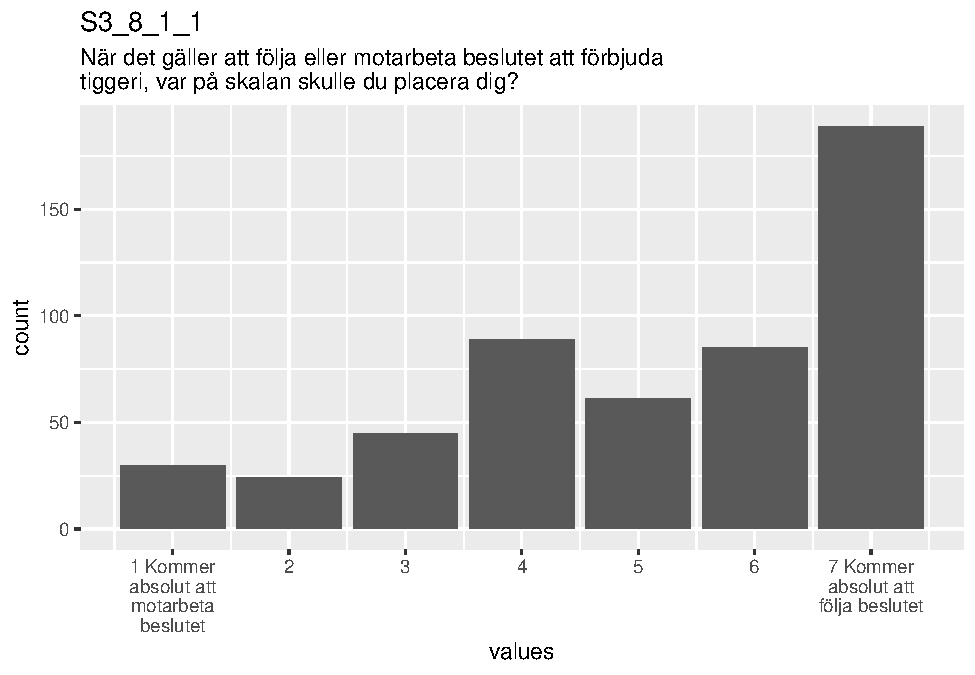
\includegraphics{Goodloser-appendix_files/figure-latex/cb_d_S3_8_1_1_distribution-1.pdf}

496 missing values.

\hypertarget{S3_8_1_1_summary}{%
\subsubsection{Summary statistics}\label{S3_8_1_1_summary}}

\begin{tabular}{l|l|l|l|r|r|l|l|l|r|r|r|l|l|l}
\hline
name & label & data_type & value_labels & n_missing & complete_rate & min & median & max & mean & sd & n_value_labels & hist & format.spss & display_width\\
\hline
S3_8_1_1 & När det gäller att följa eller motarbeta beslutet att förbjuda tiggeri, var på skalan skulle du placera dig? & haven_labelled & 1. 1 Kommer absolut att motarbeta beslutet,<br>2. 2,<br>3. 3,<br>4. 4,<br>5. 5,<br>6. 6,<br>7. 7 Kommer absolut att följa beslutet & 496 & 0.5132 & 1 & 6 & 7 & 5.176 & 1.852 & 7 & ▁▁▂▃▁▂▃▇ & F1.0 & 12\\
\hline
\end{tabular}

\hypertarget{S3_8_1_1_labels}{%
\subsubsection{Value labels}\label{S3_8_1_1_labels}}

\begin{itemize}
\tightlist
\item
  \textbf{1 Kommer absolut att motarbeta beslutet}: \emph{1}
\item
  \textbf{2}: \emph{2}
\item
  \textbf{3}: \emph{3}
\item
  \textbf{4}: \emph{4}
\item
  \textbf{5}: \emph{5}
\item
  \textbf{6}: \emph{6}
\item
  \textbf{7 Kommer absolut att följa beslutet}: \emph{7}
\end{itemize}

\hypertarget{S3_8_1_2}{%
\subsection{S3\_8\_1\_2}\label{S3_8_1_2}}

När det gäller att följa eller motarbeta beslutet att inte förbjuda tiggeri, var på skalan skulle du placera dig?

\hypertarget{S3_8_1_2_distribution}{%
\subsubsection{Distribution}\label{S3_8_1_2_distribution}}

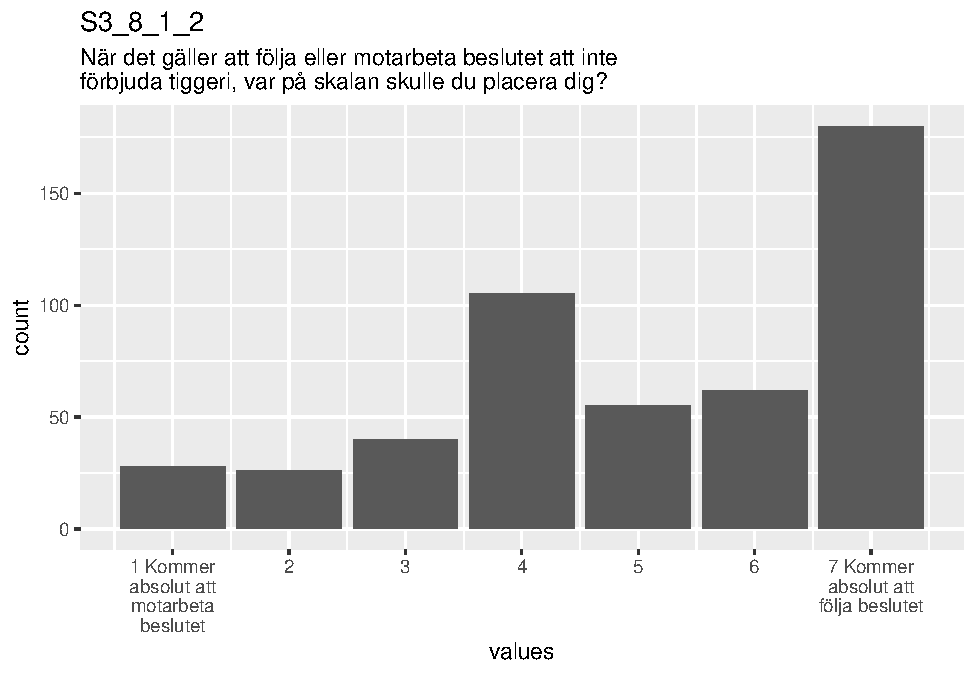
\includegraphics{Goodloser-appendix_files/figure-latex/cb_d_S3_8_1_2_distribution-1.pdf}

523 missing values.

\hypertarget{S3_8_1_2_summary}{%
\subsubsection{Summary statistics}\label{S3_8_1_2_summary}}

\begin{tabular}{l|l|l|l|r|r|l|l|l|r|r|r|l|l}
\hline
name & label & data_type & value_labels & n_missing & complete_rate & min & median & max & mean & sd & n_value_labels & hist & format.spss\\
\hline
S3_8_1_2 & När det gäller att följa eller motarbeta beslutet att inte förbjuda tiggeri, var på skalan skulle du placera dig? & haven_labelled & 1. 1 Kommer absolut att motarbeta beslutet,<br>2. 2,<br>3. 3,<br>4. 4,<br>5. 5,<br>6. 6,<br>7. 7 Kommer absolut att följa beslutet & 523 & 0.4868 & 1 & 5 & 7 & 5.095 & 1.867 & 7 & ▁▁▂▅▁▂▃▇ & F1.0\\
\hline
\end{tabular}

\hypertarget{S3_8_1_2_labels}{%
\subsubsection{Value labels}\label{S3_8_1_2_labels}}

\begin{itemize}
\tightlist
\item
  \textbf{1 Kommer absolut att motarbeta beslutet}: \emph{1}
\item
  \textbf{2}: \emph{2}
\item
  \textbf{3}: \emph{3}
\item
  \textbf{4}: \emph{4}
\item
  \textbf{5}: \emph{5}
\item
  \textbf{6}: \emph{6}
\item
  \textbf{7 Kommer absolut att följa beslutet}: \emph{7}
\end{itemize}

\hypertarget{Studie3sel}{%
\subsection{Studie3sel}\label{Studie3sel}}

Manipulation

\hypertarget{Studie3sel_distribution}{%
\subsubsection{Distribution}\label{Studie3sel_distribution}}

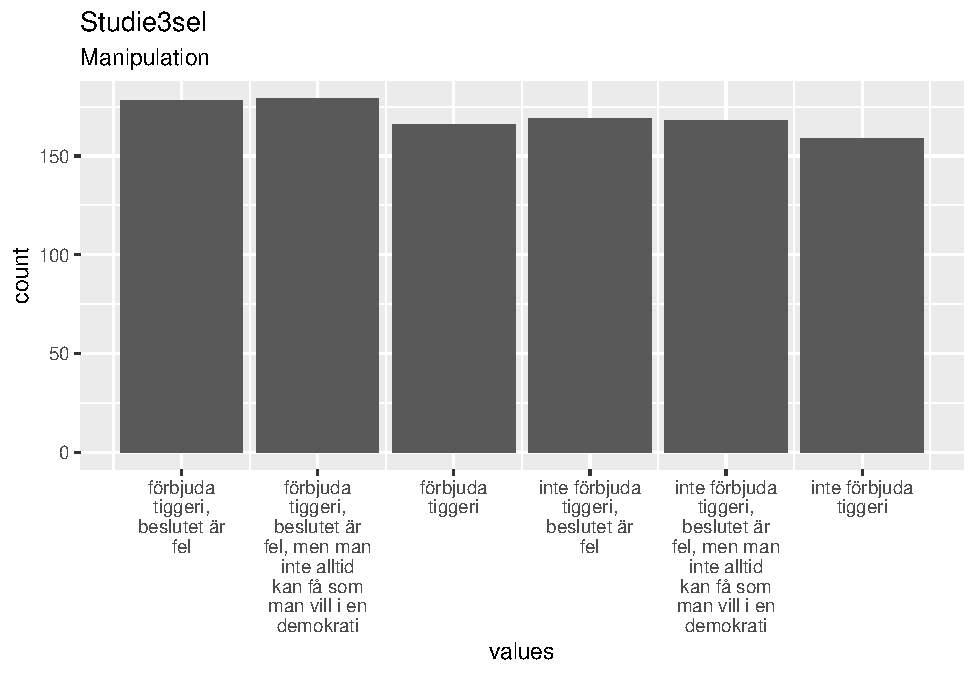
\includegraphics{Goodloser-appendix_files/figure-latex/cb_d_Studie3sel_distribution-1.pdf}

0 missing values.

\hypertarget{Studie3sel_summary}{%
\subsubsection{Summary statistics}\label{Studie3sel_summary}}

\begin{tabular}{l|l|l|l|r|r|l|l|l|r|r|r|l|l|l}
\hline
name & label & data_type & value_labels & n_missing & complete_rate & min & median & max & mean & sd & n_value_labels & hist & format.spss & display_width\\
\hline
Studie3sel & Manipulation & haven_labelled & 1. förbjuda tiggeri, beslutet är fel,<br>2. förbjuda tiggeri, beslutet är fel, men man inte alltid kan få som man vill i en demokrati,<br>3. förbjuda tiggeri,<br>4. inte förbjuda tiggeri, beslutet är fel,<br>5. inte förbjuda tiggeri, beslutet är fel, men man inte alltid kan få som man vill i en demokrati,<br>6. inte förbjuda tiggeri & 0 & 1 & 1 & 3 & 6 & 3.439 & 1.707 & 6 & ▇▇▁▇▇▁▇▇ & F1.0 & 12\\
\hline
\end{tabular}

\hypertarget{Studie3sel_labels}{%
\subsubsection{Value labels}\label{Studie3sel_labels}}

\begin{itemize}
\tightlist
\item
  \textbf{förbjuda tiggeri, beslutet är fel}: \emph{1}
\item
  \textbf{förbjuda tiggeri, beslutet är fel, men man inte alltid kan få som man vill i en demokrati}: \emph{2}
\item
  \textbf{förbjuda tiggeri}: \emph{3}
\item
  \textbf{inte förbjuda tiggeri, beslutet är fel}: \emph{4}
\item
  \textbf{inte förbjuda tiggeri, beslutet är fel, men man inte alltid kan få som man vill i en demokrati}: \emph{5}
\item
  \textbf{inte förbjuda tiggeri}: \emph{6}
\end{itemize}

\hypertarget{missingness-report}{%
\section{Missingness report}\label{missingness-report}}

\begin{tabular}{l|r|r|r|r|r|r|r|r|r|r|r}
\hline
description & Q64 & S3\_4\_1\_1 & S3\_6\_1\_1 & S3\_7\_1\_1 & S3\_8\_1\_1 & S3\_4\_1\_2 & S3\_6\_1\_2 & S3\_7\_1\_2 & S3\_8\_1\_2 & var\_miss & n\_miss\\
\hline
Missing values per variable & 4 & 496 & 496 & 496 & 496 & 523 & 523 & 523 & 523 & 4080 & 4080\\
\hline
Missing values in 4 variables & 1 & 1 & 1 & 1 & 1 & 0 & 0 & 0 & 0 & 4 & 522\\
\hline
Missing values in 4 variables & 1 & 0 & 0 & 0 & 0 & 1 & 1 & 1 & 1 & 4 & 493\\
\hline
2 other, less frequent patterns & 0 & 1 & 1 & 1 & 1 & 1 & 1 & 1 & 1 & 10 & 4\\
\hline
\end{tabular}

\hypertarget{codebook-table}{%
\section{Codebook table}\label{codebook-table}}

\begin{verbatim}
## PhantomJS not found. You can install it with webshot::install_phantomjs(). If it is installed, please make sure the phantomjs executable can be found via the PATH variable.
\end{verbatim}

\hypertarget{htmlwidget-1f9776313d0adbfaabaf}{}

JSON-LD metadata
The following JSON-LD can be found by search engines, if you share this codebook
publicly on the web.

\begin{Shaded}
\begin{Highlighting}[]
\FunctionTok{\{}
  \DataTypeTok{"name"}\FunctionTok{:} \StringTok{"d"}\FunctionTok{,}
  \DataTypeTok{"datePublished"}\FunctionTok{:} \StringTok{"2020-04-06"}\FunctionTok{,}
  \DataTypeTok{"description"}\FunctionTok{:} \StringTok{"The dataset has N=1019 rows and 14 columns.}\CharTok{\textbackslash{}n}\StringTok{0 rows have no missing values on any column.}\CharTok{\textbackslash{}n\textbackslash{}n\textbackslash{}n}\StringTok{## Table of variables}\CharTok{\textbackslash{}n}\StringTok{This table contains variable names, labels, and number of missing values.}\CharTok{\textbackslash{}n}\StringTok{See the complete codebook for more.}\CharTok{\textbackslash{}n\textbackslash{}n}\StringTok{|name       |label                                                                                                                                                          | n_missing|}\CharTok{\textbackslash{}n}\StringTok{|:----------|:--------------------------------------------------------------------------------------------------------------------------------------------------------------|---------:|}\CharTok{\textbackslash{}n}\StringTok{|Q64        |Ålder                                                                                                                                                          |         4|}\CharTok{\textbackslash{}n}\StringTok{|Q63        |Kön                                                                                                                                                            |         0|}\CharTok{\textbackslash{}n}\StringTok{|S3_1_1     |I debatten diskuteras ibland att kommunerna skall kunna förbjuda tiggeri inom sina gränser. Vad tycker du själv om att förbjuda tiggeri i kommunen där du bor? |         0|}\CharTok{\textbackslash{}n}\StringTok{|S3_2_1     |Hur viktig är frågan för dig personligen?                                                                                                                      |         0|}\CharTok{\textbackslash{}n}\StringTok{|S3_4_1_1   |Hur rättvist tycker du att det gick till när det fattades beslut om att förbjuda tiggeri?                                                                      |       496|}\CharTok{\textbackslash{}n}\StringTok{|S3_4_1_2   |Hur rättvist tycker du att det gick till när det fattades beslut om att inte förbjuda tiggeri?                                                                 |       523|}\CharTok{\textbackslash{}n}\StringTok{|S3_5_1     |Och hur schysst tycker du att beslutsproceduren var?                                                                                                           |         0|}\CharTok{\textbackslash{}n}\StringTok{|S3_6_1_1   |Och om du tänker på själva beslutet att förbjuda tiggeri. Vad tycker Du allmänt sett om beslutet?                                                              |       496|}\CharTok{\textbackslash{}n}\StringTok{|S3_6_1_2   |Och om du tänker på själva beslutet att inte förbjuda tiggeri. Vad tycker Du allmänt sett om beslutet?                                                         |       523|}\CharTok{\textbackslash{}n}\StringTok{|S3_7_1_1   |Hur villig är du att acceptera och följa beslutet att förbjuda tiggeri?                                                                                        |       496|}\CharTok{\textbackslash{}n}\StringTok{|S3_7_1_2   |Hur villig är du att acceptera och följa beslutet att inte förbjuda tiggeri?                                                                                   |       523|}\CharTok{\textbackslash{}n}\StringTok{|S3_8_1_1   |När det gäller att följa eller motarbeta beslutet att förbjuda tiggeri, var på skalan skulle du placera dig?                                                   |       496|}\CharTok{\textbackslash{}n}\StringTok{|S3_8_1_2   |När det gäller att följa eller motarbeta beslutet att inte förbjuda tiggeri, var på skalan skulle du placera dig?                                              |       523|}\CharTok{\textbackslash{}n}\StringTok{|Studie3sel |Manipulation                                                                                                                                                   |         0|}\CharTok{\textbackslash{}n\textbackslash{}n}\StringTok{### Note}\CharTok{\textbackslash{}n}\StringTok{This dataset was automatically described using the [codebook R package](https://rubenarslan.github.io/codebook/) (version 0.8.2)."}\FunctionTok{,}
  \DataTypeTok{"keywords"}\FunctionTok{:} \OtherTok{[}\StringTok{"Q64"}\OtherTok{,} \StringTok{"Q63"}\OtherTok{,} \StringTok{"S3_1_1"}\OtherTok{,} \StringTok{"S3_2_1"}\OtherTok{,} \StringTok{"S3_4_1_1"}\OtherTok{,} \StringTok{"S3_4_1_2"}\OtherTok{,} \StringTok{"S3_5_1"}\OtherTok{,} \StringTok{"S3_6_1_1"}\OtherTok{,} \StringTok{"S3_6_1_2"}\OtherTok{,} \StringTok{"S3_7_1_1"}\OtherTok{,} \StringTok{"S3_7_1_2"}\OtherTok{,} \StringTok{"S3_8_1_1"}\OtherTok{,} \StringTok{"S3_8_1_2"}\OtherTok{,} \StringTok{"Studie3sel"}\OtherTok{]}\FunctionTok{,}
  \DataTypeTok{"@context"}\FunctionTok{:} \StringTok{"http://schema.org/"}\FunctionTok{,}
  \DataTypeTok{"@type"}\FunctionTok{:} \StringTok{"Dataset"}\FunctionTok{,}
  \DataTypeTok{"variableMeasured"}\FunctionTok{:} \OtherTok{[}
    \FunctionTok{\{}
      \DataTypeTok{"name"}\FunctionTok{:} \StringTok{"Q64"}\FunctionTok{,}
      \DataTypeTok{"description"}\FunctionTok{:} \StringTok{"Ålder"}\FunctionTok{,}
      \DataTypeTok{"@type"}\FunctionTok{:} \StringTok{"propertyValue"}
    \FunctionTok{\}}\OtherTok{,}
    \FunctionTok{\{}
      \DataTypeTok{"name"}\FunctionTok{:} \StringTok{"Q63"}\FunctionTok{,}
      \DataTypeTok{"description"}\FunctionTok{:} \StringTok{"Kön"}\FunctionTok{,}
      \DataTypeTok{"value"}\FunctionTok{:} \StringTok{"1. Man,}\CharTok{\textbackslash{}n}\StringTok{2. Kvinna"}\FunctionTok{,}
      \DataTypeTok{"maxValue"}\FunctionTok{:} \DecValTok{2}\FunctionTok{,}
      \DataTypeTok{"minValue"}\FunctionTok{:} \DecValTok{1}\FunctionTok{,}
      \DataTypeTok{"@type"}\FunctionTok{:} \StringTok{"propertyValue"}
    \FunctionTok{\}}\OtherTok{,}
    \FunctionTok{\{}
      \DataTypeTok{"name"}\FunctionTok{:} \StringTok{"S3_1_1"}\FunctionTok{,}
      \DataTypeTok{"description"}\FunctionTok{:} \StringTok{"I debatten diskuteras ibland att kommunerna skall kunna förbjuda tiggeri inom sina gränser. Vad tycker du själv om att förbjuda tiggeri i kommunen där du bor?"}\FunctionTok{,}
      \DataTypeTok{"value"}\FunctionTok{:} \StringTok{"1. Jag är huvudsakligen emot att förbjuda tiggeri i min kommun,}\CharTok{\textbackslash{}n}\StringTok{2. Jag är huvudsakligen för att förbjuda tiggeri i min kommun"}\FunctionTok{,}
      \DataTypeTok{"maxValue"}\FunctionTok{:} \DecValTok{2}\FunctionTok{,}
      \DataTypeTok{"minValue"}\FunctionTok{:} \DecValTok{1}\FunctionTok{,}
      \DataTypeTok{"@type"}\FunctionTok{:} \StringTok{"propertyValue"}
    \FunctionTok{\}}\OtherTok{,}
    \FunctionTok{\{}
      \DataTypeTok{"name"}\FunctionTok{:} \StringTok{"S3_2_1"}\FunctionTok{,}
      \DataTypeTok{"description"}\FunctionTok{:} \StringTok{"Hur viktig är frågan för dig personligen?"}\FunctionTok{,}
      \DataTypeTok{"value"}\FunctionTok{:} \StringTok{"1. 1 Inte alls viktig,}\CharTok{\textbackslash{}n}\StringTok{2. 2,}\CharTok{\textbackslash{}n}\StringTok{3. 3,}\CharTok{\textbackslash{}n}\StringTok{4. 4,}\CharTok{\textbackslash{}n}\StringTok{5. 5,}\CharTok{\textbackslash{}n}\StringTok{6. 6,}\CharTok{\textbackslash{}n}\StringTok{7. 7 Mycket viktig"}\FunctionTok{,}
      \DataTypeTok{"maxValue"}\FunctionTok{:} \DecValTok{7}\FunctionTok{,}
      \DataTypeTok{"minValue"}\FunctionTok{:} \DecValTok{1}\FunctionTok{,}
      \DataTypeTok{"@type"}\FunctionTok{:} \StringTok{"propertyValue"}
    \FunctionTok{\}}\OtherTok{,}
    \FunctionTok{\{}
      \DataTypeTok{"name"}\FunctionTok{:} \StringTok{"S3_4_1_1"}\FunctionTok{,}
      \DataTypeTok{"description"}\FunctionTok{:} \StringTok{"Hur rättvist tycker du att det gick till när det fattades beslut om att förbjuda tiggeri?"}\FunctionTok{,}
      \DataTypeTok{"value"}\FunctionTok{:} \StringTok{"1. 1 Inte alls rättvist,}\CharTok{\textbackslash{}n}\StringTok{2. 2,}\CharTok{\textbackslash{}n}\StringTok{3. 3,}\CharTok{\textbackslash{}n}\StringTok{4. 4,}\CharTok{\textbackslash{}n}\StringTok{5. 5,}\CharTok{\textbackslash{}n}\StringTok{6. 6,}\CharTok{\textbackslash{}n}\StringTok{7. 7 Mycket rättvist"}\FunctionTok{,}
      \DataTypeTok{"maxValue"}\FunctionTok{:} \DecValTok{7}\FunctionTok{,}
      \DataTypeTok{"minValue"}\FunctionTok{:} \DecValTok{1}\FunctionTok{,}
      \DataTypeTok{"@type"}\FunctionTok{:} \StringTok{"propertyValue"}
    \FunctionTok{\}}\OtherTok{,}
    \FunctionTok{\{}
      \DataTypeTok{"name"}\FunctionTok{:} \StringTok{"S3_4_1_2"}\FunctionTok{,}
      \DataTypeTok{"description"}\FunctionTok{:} \StringTok{"Hur rättvist tycker du att det gick till när det fattades beslut om att inte förbjuda tiggeri?"}\FunctionTok{,}
      \DataTypeTok{"value"}\FunctionTok{:} \StringTok{"1. 1 Inte alls rättvist,}\CharTok{\textbackslash{}n}\StringTok{2. 2,}\CharTok{\textbackslash{}n}\StringTok{3. 3,}\CharTok{\textbackslash{}n}\StringTok{4. 4,}\CharTok{\textbackslash{}n}\StringTok{5. 5,}\CharTok{\textbackslash{}n}\StringTok{6. 6,}\CharTok{\textbackslash{}n}\StringTok{7. 7 Mycket rättvist"}\FunctionTok{,}
      \DataTypeTok{"maxValue"}\FunctionTok{:} \DecValTok{7}\FunctionTok{,}
      \DataTypeTok{"minValue"}\FunctionTok{:} \DecValTok{1}\FunctionTok{,}
      \DataTypeTok{"@type"}\FunctionTok{:} \StringTok{"propertyValue"}
    \FunctionTok{\}}\OtherTok{,}
    \FunctionTok{\{}
      \DataTypeTok{"name"}\FunctionTok{:} \StringTok{"S3_5_1"}\FunctionTok{,}
      \DataTypeTok{"description"}\FunctionTok{:} \StringTok{"Och hur schysst tycker du att beslutsproceduren var?"}\FunctionTok{,}
      \DataTypeTok{"value"}\FunctionTok{:} \StringTok{"1. 1 Mycket oschysst,}\CharTok{\textbackslash{}n}\StringTok{2. 2,}\CharTok{\textbackslash{}n}\StringTok{3. 3,}\CharTok{\textbackslash{}n}\StringTok{4. 4,}\CharTok{\textbackslash{}n}\StringTok{5. 5,}\CharTok{\textbackslash{}n}\StringTok{6. 6,}\CharTok{\textbackslash{}n}\StringTok{7. 7 Mycket schysst"}\FunctionTok{,}
      \DataTypeTok{"maxValue"}\FunctionTok{:} \DecValTok{7}\FunctionTok{,}
      \DataTypeTok{"minValue"}\FunctionTok{:} \DecValTok{1}\FunctionTok{,}
      \DataTypeTok{"@type"}\FunctionTok{:} \StringTok{"propertyValue"}
    \FunctionTok{\}}\OtherTok{,}
    \FunctionTok{\{}
      \DataTypeTok{"name"}\FunctionTok{:} \StringTok{"S3_6_1_1"}\FunctionTok{,}
      \DataTypeTok{"description"}\FunctionTok{:} \StringTok{"Och om du tänker på själva beslutet att förbjuda tiggeri. Vad tycker Du allmänt sett om beslutet?"}\FunctionTok{,}
      \DataTypeTok{"value"}\FunctionTok{:} \StringTok{"1. 1 Mycket dåligt,}\CharTok{\textbackslash{}n}\StringTok{2. 2,}\CharTok{\textbackslash{}n}\StringTok{3. 3,}\CharTok{\textbackslash{}n}\StringTok{4. 4,}\CharTok{\textbackslash{}n}\StringTok{5. 5,}\CharTok{\textbackslash{}n}\StringTok{6. 6,}\CharTok{\textbackslash{}n}\StringTok{7. 7 Mycket bra"}\FunctionTok{,}
      \DataTypeTok{"maxValue"}\FunctionTok{:} \DecValTok{7}\FunctionTok{,}
      \DataTypeTok{"minValue"}\FunctionTok{:} \DecValTok{1}\FunctionTok{,}
      \DataTypeTok{"@type"}\FunctionTok{:} \StringTok{"propertyValue"}
    \FunctionTok{\}}\OtherTok{,}
    \FunctionTok{\{}
      \DataTypeTok{"name"}\FunctionTok{:} \StringTok{"S3_6_1_2"}\FunctionTok{,}
      \DataTypeTok{"description"}\FunctionTok{:} \StringTok{"Och om du tänker på själva beslutet att inte förbjuda tiggeri. Vad tycker Du allmänt sett om beslutet?"}\FunctionTok{,}
      \DataTypeTok{"value"}\FunctionTok{:} \StringTok{"1. 1 Mycket dåligt,}\CharTok{\textbackslash{}n}\StringTok{2. 2,}\CharTok{\textbackslash{}n}\StringTok{3. 3,}\CharTok{\textbackslash{}n}\StringTok{4. 4,}\CharTok{\textbackslash{}n}\StringTok{5. 5,}\CharTok{\textbackslash{}n}\StringTok{6. 6,}\CharTok{\textbackslash{}n}\StringTok{7. 7 Mycket bra"}\FunctionTok{,}
      \DataTypeTok{"maxValue"}\FunctionTok{:} \DecValTok{7}\FunctionTok{,}
      \DataTypeTok{"minValue"}\FunctionTok{:} \DecValTok{1}\FunctionTok{,}
      \DataTypeTok{"@type"}\FunctionTok{:} \StringTok{"propertyValue"}
    \FunctionTok{\}}\OtherTok{,}
    \FunctionTok{\{}
      \DataTypeTok{"name"}\FunctionTok{:} \StringTok{"S3_7_1_1"}\FunctionTok{,}
      \DataTypeTok{"description"}\FunctionTok{:} \StringTok{"Hur villig är du att acceptera och följa beslutet att förbjuda tiggeri?"}\FunctionTok{,}
      \DataTypeTok{"value"}\FunctionTok{:} \StringTok{"1. 1 Inte alls villig,}\CharTok{\textbackslash{}n}\StringTok{2. 2,}\CharTok{\textbackslash{}n}\StringTok{3. 3,}\CharTok{\textbackslash{}n}\StringTok{4. 4,}\CharTok{\textbackslash{}n}\StringTok{5. 5,}\CharTok{\textbackslash{}n}\StringTok{6. 6,}\CharTok{\textbackslash{}n}\StringTok{7. 7 Mycket villig"}\FunctionTok{,}
      \DataTypeTok{"maxValue"}\FunctionTok{:} \DecValTok{7}\FunctionTok{,}
      \DataTypeTok{"minValue"}\FunctionTok{:} \DecValTok{1}\FunctionTok{,}
      \DataTypeTok{"@type"}\FunctionTok{:} \StringTok{"propertyValue"}
    \FunctionTok{\}}\OtherTok{,}
    \FunctionTok{\{}
      \DataTypeTok{"name"}\FunctionTok{:} \StringTok{"S3_7_1_2"}\FunctionTok{,}
      \DataTypeTok{"description"}\FunctionTok{:} \StringTok{"Hur villig är du att acceptera och följa beslutet att inte förbjuda tiggeri?"}\FunctionTok{,}
      \DataTypeTok{"value"}\FunctionTok{:} \StringTok{"1. 1 Inte alls villig,}\CharTok{\textbackslash{}n}\StringTok{2. 2,}\CharTok{\textbackslash{}n}\StringTok{3. 3,}\CharTok{\textbackslash{}n}\StringTok{4. 4,}\CharTok{\textbackslash{}n}\StringTok{5. 5,}\CharTok{\textbackslash{}n}\StringTok{6. 6,}\CharTok{\textbackslash{}n}\StringTok{7. 7 Mycket villig"}\FunctionTok{,}
      \DataTypeTok{"maxValue"}\FunctionTok{:} \DecValTok{7}\FunctionTok{,}
      \DataTypeTok{"minValue"}\FunctionTok{:} \DecValTok{1}\FunctionTok{,}
      \DataTypeTok{"@type"}\FunctionTok{:} \StringTok{"propertyValue"}
    \FunctionTok{\}}\OtherTok{,}
    \FunctionTok{\{}
      \DataTypeTok{"name"}\FunctionTok{:} \StringTok{"S3_8_1_1"}\FunctionTok{,}
      \DataTypeTok{"description"}\FunctionTok{:} \StringTok{"När det gäller att följa eller motarbeta beslutet att förbjuda tiggeri, var på skalan skulle du placera dig?"}\FunctionTok{,}
      \DataTypeTok{"value"}\FunctionTok{:} \StringTok{"1. 1 Kommer absolut att motarbeta beslutet,}\CharTok{\textbackslash{}n}\StringTok{2. 2,}\CharTok{\textbackslash{}n}\StringTok{3. 3,}\CharTok{\textbackslash{}n}\StringTok{4. 4,}\CharTok{\textbackslash{}n}\StringTok{5. 5,}\CharTok{\textbackslash{}n}\StringTok{6. 6,}\CharTok{\textbackslash{}n}\StringTok{7. 7 Kommer absolut att följa beslutet"}\FunctionTok{,}
      \DataTypeTok{"maxValue"}\FunctionTok{:} \DecValTok{7}\FunctionTok{,}
      \DataTypeTok{"minValue"}\FunctionTok{:} \DecValTok{1}\FunctionTok{,}
      \DataTypeTok{"@type"}\FunctionTok{:} \StringTok{"propertyValue"}
    \FunctionTok{\}}\OtherTok{,}
    \FunctionTok{\{}
      \DataTypeTok{"name"}\FunctionTok{:} \StringTok{"S3_8_1_2"}\FunctionTok{,}
      \DataTypeTok{"description"}\FunctionTok{:} \StringTok{"När det gäller att följa eller motarbeta beslutet att inte förbjuda tiggeri, var på skalan skulle du placera dig?"}\FunctionTok{,}
      \DataTypeTok{"value"}\FunctionTok{:} \StringTok{"1. 1 Kommer absolut att motarbeta beslutet,}\CharTok{\textbackslash{}n}\StringTok{2. 2,}\CharTok{\textbackslash{}n}\StringTok{3. 3,}\CharTok{\textbackslash{}n}\StringTok{4. 4,}\CharTok{\textbackslash{}n}\StringTok{5. 5,}\CharTok{\textbackslash{}n}\StringTok{6. 6,}\CharTok{\textbackslash{}n}\StringTok{7. 7 Kommer absolut att följa beslutet"}\FunctionTok{,}
      \DataTypeTok{"maxValue"}\FunctionTok{:} \DecValTok{7}\FunctionTok{,}
      \DataTypeTok{"minValue"}\FunctionTok{:} \DecValTok{1}\FunctionTok{,}
      \DataTypeTok{"@type"}\FunctionTok{:} \StringTok{"propertyValue"}
    \FunctionTok{\}}\OtherTok{,}
    \FunctionTok{\{}
      \DataTypeTok{"name"}\FunctionTok{:} \StringTok{"Studie3sel"}\FunctionTok{,}
      \DataTypeTok{"description"}\FunctionTok{:} \StringTok{"Manipulation"}\FunctionTok{,}
      \DataTypeTok{"value"}\FunctionTok{:} \StringTok{"1. förbjuda tiggeri, beslutet är fel,}\CharTok{\textbackslash{}n}\StringTok{2. förbjuda tiggeri, beslutet är fel, men man inte alltid kan få som man vill i en demokrati,}\CharTok{\textbackslash{}n}\StringTok{3. förbjuda tiggeri,}\CharTok{\textbackslash{}n}\StringTok{4. inte förbjuda tiggeri, beslutet är fel,}\CharTok{\textbackslash{}n}\StringTok{5. inte förbjuda tiggeri, beslutet är fel, men man inte alltid kan få som man vill i en demokrati,}\CharTok{\textbackslash{}n}\StringTok{6. inte förbjuda tiggeri"}\FunctionTok{,}
      \DataTypeTok{"maxValue"}\FunctionTok{:} \DecValTok{6}\FunctionTok{,}
      \DataTypeTok{"minValue"}\FunctionTok{:} \DecValTok{1}\FunctionTok{,}
      \DataTypeTok{"@type"}\FunctionTok{:} \StringTok{"propertyValue"}
    \FunctionTok{\}}
  \OtherTok{]}
\FunctionTok{\}}\ErrorTok{`}
\end{Highlighting}
\end{Shaded}

\hypertarget{part-study-ii-norwegian-vignette}{%
\part{STUDY II: NORWEGIAN VIGNETTE}\label{part-study-ii-norwegian-vignette}}

\hypertarget{data-management-1}{%
\chapter{Data management}\label{data-management-1}}

\begin{quote}
Script for data management that is conducted prior to any analysis.
\end{quote}

\begin{Shaded}
\begin{Highlighting}[]
\NormalTok{d <-}\StringTok{ }\NormalTok{d }\OperatorTok
\StringTok{  }\KeywordTok{rename}\NormalTok{(}\StringTok{"imp_accept"}\NormalTok{=}\StringTok{ "r9pad1"}\NormalTok{,}
          \StringTok{"other_accept"}\NormalTok{ =}\StringTok{ "r9pad2"}\NormalTok{,}
          \StringTok{"self_accept"}\NormalTok{ =}\StringTok{ "r9pad3"}\NormalTok{,}
          \StringTok{"opinion_ban"}\NormalTok{ =}\StringTok{ "r10pad1"}\NormalTok{,}
          \StringTok{"opinion_strength"}\NormalTok{ =}\StringTok{ "r10pad2"}\NormalTok{,}
          \StringTok{"video_mobile"}\NormalTok{ =}\StringTok{ "r10pad3_mobil"}\NormalTok{,}
          \StringTok{"video_proban_treat"}\NormalTok{ =}\StringTok{ "r10pad3a_ran"}\NormalTok{,}
          \StringTok{"video_antiban_treat"}\NormalTok{ =}\StringTok{ "r10pad3b_ran"}\NormalTok{,}
          \StringTok{"video_ended"}\NormalTok{ =}\StringTok{ "r10pad3ended"}\NormalTok{,}
          \StringTok{"video_error"}\NormalTok{ =}\StringTok{ "r10pad3error"}\NormalTok{,}
          \StringTok{"video_paused"}\NormalTok{ =}\StringTok{ "r10pad3paused"}\NormalTok{,}
          \StringTok{"video_played"}\NormalTok{ =}\StringTok{ "r10pad3played"}\NormalTok{,}
          \StringTok{"video_timespent"}\NormalTok{ =}\StringTok{ "r10pad3_timespent"}\NormalTok{,}
          \StringTok{"video_report"}\NormalTok{ =}\StringTok{ "r10pad4"}\NormalTok{,}
          \StringTok{"fairness"}\NormalTok{ =}\StringTok{ "r10pad5"}\NormalTok{,}
          \StringTok{"accept"}\NormalTok{ =}\StringTok{ "r10pad6"}\NormalTok{,}
          \StringTok{"trust"}\NormalTok{ =}\StringTok{ "r10pad7"}\NormalTok{,}
          \StringTok{"check_outcome"}\NormalTok{ =}\StringTok{ "r10pad8"}\NormalTok{,}
          \StringTok{"check_politician"}\NormalTok{ =}\StringTok{ "r10pad9"}
\NormalTok{  )}

\CommentTok{#Merge treatments with ban and no ban outcomes          }
\NormalTok{d <-}\StringTok{ }\NormalTok{d }\OperatorTok
\StringTok{  }\KeywordTok{gather}\NormalTok{(video, treatment, video_proban_treat}\OperatorTok{:}\NormalTok{video_antiban_treat)}

\CommentTok{#Make NA the respondents with values 98 (Not asked) or 97 (No answer) for entire dataset. (Checked with command 'sum(is.na(Loser$video_timespent)) that no values on that }
\CommentTok{#variable has value 97 or 98)}
\NormalTok{d[d }\OperatorTok{==}\StringTok{ }\DecValTok{97}\NormalTok{] <-}\StringTok{ }\OtherTok{NA}
\NormalTok{d[d }\OperatorTok{==}\StringTok{ }\DecValTok{98}\NormalTok{] <-}\StringTok{ }\OtherTok{NA}

\CommentTok{#Reverse scales}
\NormalTok{d <-}\StringTok{ }\NormalTok{d }\OperatorTok
\StringTok{  }\KeywordTok{mutate}\NormalTok{(}\DataTypeTok{imp_accept =} \OperatorTok{-}\NormalTok{(imp_accept)}\OperatorTok{+}\DecValTok{6}\NormalTok{,}
         \DataTypeTok{other_accept =} \OperatorTok{-}\NormalTok{(other_accept)}\OperatorTok{+}\DecValTok{6}\NormalTok{,}
         \DataTypeTok{self_accept =} \OperatorTok{-}\NormalTok{(self_accept)}\OperatorTok{+}\DecValTok{6}\NormalTok{,}
         \DataTypeTok{opinion_strength =} \OperatorTok{-}\NormalTok{(opinion_strength)}\OperatorTok{+}\DecValTok{6}\NormalTok{,}
         \DataTypeTok{fairness =} \OperatorTok{-}\NormalTok{(fairness)}\OperatorTok{+}\DecValTok{6}\NormalTok{,}
         \DataTypeTok{accept =} \OperatorTok{-}\NormalTok{(accept)}\OperatorTok{+}\DecValTok{6}\NormalTok{,}
         \DataTypeTok{trust =} \OperatorTok{-}\NormalTok{(trust)}\OperatorTok{+}\DecValTok{6}
\NormalTok{  )}


\CommentTok{##Create manipulation check variable that measures whether the respondents correctly identify whether the outcome was favorable or unfavorable to them}
\NormalTok{d <-}\StringTok{ }\NormalTok{d }\OperatorTok
\StringTok{  }\KeywordTok{mutate}\NormalTok{(}\DataTypeTok{favorability =} \KeywordTok{case_when}\NormalTok{(}
\NormalTok{    treatment }\OperatorTok\StringTok{ }\DecValTok{1}\OperatorTok{:}\DecValTok{4} \OperatorTok{~}\StringTok{ "Unfavorable"}\NormalTok{,}
\NormalTok{    treatment }\OperatorTok{==}\StringTok{ }\DecValTok{5}    \OperatorTok{~}\StringTok{ "Favorable"}
\NormalTok{  )}
\NormalTok{  )}\OperatorTok
\StringTok{  }\KeywordTok{mutate}\NormalTok{(}\DataTypeTok{mcheck_favorability =} \KeywordTok{case_when}\NormalTok{(}
    \KeywordTok{is.na}\NormalTok{(favorability) }\OperatorTok{~}\StringTok{ "Incorrect"}\NormalTok{,}
\NormalTok{    favorability}\OperatorTok{==}\StringTok{"Favorable"} \OperatorTok{&}\StringTok{ }\NormalTok{check_outcome}\OperatorTok{==}\DecValTok{1} \OperatorTok{~}\StringTok{ "Correct"}\NormalTok{,}
\NormalTok{    favorability}\OperatorTok{==}\StringTok{"Unfavorable"} \OperatorTok{&}\StringTok{ }\NormalTok{check_outcome}\OperatorTok{==}\DecValTok{2} \OperatorTok{~}\StringTok{ "Correct"}\NormalTok{,}
\NormalTok{    favorability }\OperatorTok\StringTok{ }\DecValTok{3}\OperatorTok{:}\DecValTok{4} \OperatorTok{~}\StringTok{ "Incorrect"}\NormalTok{,}
\NormalTok{    favorability}\OperatorTok{==}\StringTok{"Favorable"} \OperatorTok{&}\StringTok{ }\NormalTok{check_outcome}\OperatorTok{==}\DecValTok{2} \OperatorTok{~}\StringTok{ "Incorrect"}\NormalTok{,}
\NormalTok{    favorability}\OperatorTok{==}\StringTok{"Unfavorable"} \OperatorTok{&}\StringTok{ }\NormalTok{check_outcome}\OperatorTok{==}\DecValTok{1} \OperatorTok{~}\StringTok{ "Incorrect"}
\NormalTok{  )}
\NormalTok{  ) }

\CommentTok{#Label values on treatment variable}
\NormalTok{d <-}\StringTok{ }\NormalTok{d }\OperatorTok
\StringTok{  }\KeywordTok{mutate}\NormalTok{(}\DataTypeTok{treatment =} \KeywordTok{case_when}\NormalTok{(}
\NormalTok{    .[[}\StringTok{"treatment"}\NormalTok{]] }\OperatorTok{==}\StringTok{ }\DecValTok{1} \OperatorTok{~}\StringTok{ "Lamenting politician"}\NormalTok{,}
\NormalTok{    .[[}\StringTok{"treatment"}\NormalTok{]] }\OperatorTok{==}\StringTok{ }\DecValTok{2} \OperatorTok{~}\StringTok{ "Specific prime"}\NormalTok{,}
\NormalTok{    .[[}\StringTok{"treatment"}\NormalTok{]] }\OperatorTok{==}\StringTok{ }\DecValTok{3} \OperatorTok{~}\StringTok{ "General Prime"}\NormalTok{,}
\NormalTok{    .[[}\StringTok{"treatment"}\NormalTok{]] }\OperatorTok{==}\StringTok{ }\DecValTok{4} \OperatorTok{~}\StringTok{ "Not shown"}\NormalTok{,}
\NormalTok{    .[[}\StringTok{"treatment"}\NormalTok{]] }\OperatorTok{==}\StringTok{ }\DecValTok{5} \OperatorTok{~}\StringTok{ "Winner"}\NormalTok{),}
    \DataTypeTok{opinion_ban =} \KeywordTok{case_when}\NormalTok{(}
\NormalTok{    .[[}\StringTok{"opinion_ban"}\NormalTok{]] }\OperatorTok{==}\StringTok{ }\DecValTok{1} \OperatorTok{~}\StringTok{ "Pro"}\NormalTok{,}
\NormalTok{    .[[}\StringTok{"opinion_ban"}\NormalTok{]] }\OperatorTok{==}\StringTok{ }\DecValTok{2} \OperatorTok{~}\StringTok{ "Anti"}\NormalTok{),}
    \DataTypeTok{responseid =} \KeywordTok{as.numeric}\NormalTok{(responseid),}
         \DataTypeTok{imp_accept2 =} \KeywordTok{case_when}\NormalTok{(imp_accept }\OperatorTok\StringTok{ }\DecValTok{4}\OperatorTok{:}\DecValTok{5} \OperatorTok{~}\StringTok{ "Important"}\NormalTok{,}
\NormalTok{                                imp_accept }\OperatorTok\StringTok{ }\DecValTok{1}\OperatorTok{:}\DecValTok{3} \OperatorTok{~}\StringTok{ "Not important"}\NormalTok{),}
         \DataTypeTok{other_accept2 =} \KeywordTok{case_when}\NormalTok{(other_accept }\OperatorTok\StringTok{ }\DecValTok{4}\OperatorTok{:}\DecValTok{5} \OperatorTok{~}\StringTok{ "High degree"}\NormalTok{,}
\NormalTok{                                  other_accept }\OperatorTok\StringTok{ }\DecValTok{1}\OperatorTok{:}\DecValTok{3} \OperatorTok{~}\StringTok{ "Low degree"}\NormalTok{),}
         \DataTypeTok{self_accept2 =} \KeywordTok{case_when}\NormalTok{(self_accept }\OperatorTok\StringTok{ }\DecValTok{4}\OperatorTok{:}\DecValTok{5} \OperatorTok{~}\StringTok{ "High degree"}\NormalTok{,}
\NormalTok{                                 self_accept }\OperatorTok\StringTok{ }\DecValTok{1}\OperatorTok{:}\DecValTok{3} \OperatorTok{~}\StringTok{ "Low degree"}\NormalTok{),}
         \DataTypeTok{opinion_strength2 =} \KeywordTok{case_when}\NormalTok{(opinion_strength }\OperatorTok\StringTok{ }\DecValTok{4}\OperatorTok{:}\DecValTok{5} \OperatorTok{~}\StringTok{ "Important"}\NormalTok{,}
\NormalTok{                                      opinion_strength }\OperatorTok\StringTok{ }\DecValTok{1}\OperatorTok{:}\DecValTok{3} \OperatorTok{~}\StringTok{ "Not important"}\NormalTok{)}
\NormalTok{  )}
\CommentTok{#----------------------------------------------------}
\CommentTok{#Prepare data sets with different samples}
\CommentTok{#----------------------------------------------------}

\CommentTok{# Keep a full ITT dataset}

\NormalTok{d <-}\StringTok{ }\NormalTok{d }\OperatorTok
\StringTok{  }\KeywordTok{filter}\NormalTok{(}\OperatorTok{!}\KeywordTok{is.na}\NormalTok{(treatment)) }\CommentTok{#Keep all who where assigned to a video treatment}

\KeywordTok{write_sav}\NormalTok{(d, }\StringTok{"Data/Goodloser-exp2-itt.sav"}\NormalTok{)}
\KeywordTok{write_csv}\NormalTok{(d, }\StringTok{"Data/Goodloser-exp2-itt.csv"}\NormalTok{)}

\CommentTok{#Remove respondents who did not see the video properly. Will be used as main data set}
\NormalTok{  d <-}\StringTok{ }\NormalTok{d }\OperatorTok\StringTok{ }\KeywordTok{filter}\NormalTok{(video_timespent }\OperatorTok\StringTok{ }\DecValTok{60}\OperatorTok{:}\DecValTok{300}\NormalTok{) }\OperatorTok\StringTok{ }\CommentTok{#Keep only those who stayed with the video for more than 60 seconds and less than 300 seconds}
\StringTok{  }\KeywordTok{filter}\NormalTok{(video_report }\OperatorTok\StringTok{ }\KeywordTok{c}\NormalTok{(}\DecValTok{1}\NormalTok{, }\DecValTok{3}\NormalTok{)) }\CommentTok{#Keep only those who reported that they had sound and picture or picture but no sound}

\KeywordTok{write_sav}\NormalTok{(d, }\StringTok{"Data/Goodloser-exp2.sav"}\NormalTok{)}
\KeywordTok{write_csv}\NormalTok{(d, }\StringTok{"Data/Goodloser-exp2.csv"}\NormalTok{)}

\CommentTok{#Create a separate data set where also those who fail the manipulation check are excluded.}
\NormalTok{Loser_redux <-}\StringTok{ }\NormalTok{d }\OperatorTok
\StringTok{  }\KeywordTok{filter}\NormalTok{(mcheck_favorability }\OperatorTok{==}\StringTok{ "Correct"}\NormalTok{)}

\CommentTok{#Save file with the good loser data set that excludes respondents who fail manipulation check}

\KeywordTok{write_sav}\NormalTok{(Loser_redux, }\StringTok{"Data/Goodloser-exp2-exclusive.sav"}\NormalTok{)}
\KeywordTok{write_csv}\NormalTok{(Loser_redux, }\StringTok{"Data/Goodloser-exp2-exclusive.csv"}\NormalTok{)}
\end{Highlighting}
\end{Shaded}

\hypertarget{pre-treatment-vignette-post-treatment}{%
\chapter{Pre-treatment, vignette, post-treatment}\label{pre-treatment-vignette-post-treatment}}

The experiment was fielded in Norway during the spring and fall of 2017 during the 9th and 10th waves of \href{https://www.uib.no/medborger}{Norwegian Citizen Panel (NCP)}. The NCP is a research-purpose internet panel with over 6000 active participants. It is based on a probability sample of the general Norwegian population above the age of 18 drawn from the Norwegian National Registry. The survey is based on a online questionnaire with postal recruitment. Panel members complete a questionnaire three times a year of 15 minutes each. The NCP is a core component of The Digital Social Science Core Facilities (DIGSSCORE), and was established in 2013 as a collaboration between several departments at the Faculty of Social Sciences at the University of Bergen and NORCE -- Norwegian Research Centre. We refer to the \href{Data/ncp-wave13-documentation.pdf}{documentation report} for further details on technical aspects of the survey, panel recruitment, response rates of the 13th wave, and representativeness. For details about the data collected in this project and the NCP at large, we refer to the \href{Data/ncp-wave13-codebook.pdf}{codebook for the Waves 1-13}.

\hypertarget{pre-treatment-measures-1}{%
\section{Pre-treatment measures}\label{pre-treatment-measures-1}}

\textbackslash begin\{table\}{[}H{]}

\textbackslash caption\{(\#tab:2031\_pre)What is your opinion -- how important is it to accept the decisions about important social issues after they have been adopted?\}
\centering

\begin{tabular}[t]{lrr}
\toprule
Value & N & Percent\\
\midrule
Not important at all & 17 & 1\\
Slightly important & 54 & 4\\
Somewhat important & 329 & 26\\
Important & 710 & 56\\
Very important & 135 & 11\\
NA & 34 & 3\\
\bottomrule
\end{tabular}

\textbackslash end\{table\}

\textbackslash begin\{table\}{[}H{]}

\textbackslash caption\{(\#tab:2031\_pre)To what extent do you think people in Norway are willing to accept the decisions about important social issues after they have been adopted by politicians and the authorities?\}
\centering

\begin{tabular}[t]{lrr}
\toprule
Value & N & Percent\\
\midrule
Not at all & 2 & 0\\
Low degree & 50 & 4\\
Some degree & 461 & 36\\
High degree & 635 & 50\\
Very high degree & 66 & 5\\
NA & 65 & 5\\
\bottomrule
\end{tabular}

\textbackslash end\{table\}

\textbackslash begin\{table\}{[}H{]}

\textbackslash caption\{(\#tab:2031\_pre)What about you personally -- do you live up to this standard (i.e., accept the decisions about important social issues after they have been adopted by politicians and the authorities)?\}
\centering

\begin{tabular}[t]{lrr}
\toprule
Value & N & Percent\\
\midrule
Not at all & 12 & 1\\
Low degree & 39 & 3\\
Some degree & 362 & 28\\
High degree & 716 & 56\\
Very high degree & 91 & 7\\
NA & 59 & 5\\
\bottomrule
\end{tabular}

\textbackslash end\{table\}

\textbackslash begin\{table\}{[}H{]}

\textbackslash caption\{(\#tab:2031\_pre)What is your opinion on a ban on begging in your municipality?\}
\centering

\begin{tabular}[t]{lrr}
\toprule
Value & N & Percent\\
\midrule
 & 22 & 2\\
Anti & 417 & 33\\
Pro & 840 & 66\\
\bottomrule
\end{tabular}

\textbackslash end\{table\}

\textbackslash begin\{table\}{[}H{]}

\textbackslash caption\{(\#tab:2031\_pre)How important is this issue to you personally?\}
\centering

\begin{tabular}[t]{lrr}
\toprule
Value & N & Percent\\
\midrule
Not important at all & 65 & 5\\
Slightly important & 444 & 35\\
Somewhat important & 418 & 33\\
Important & 236 & 18\\
Very important & 88 & 7\\
NA & 28 & 2\\
\bottomrule
\end{tabular}

\textbackslash end\{table\}

\hypertarget{experimental-vignette-1}{%
\section{Experimental vignette}\label{experimental-vignette-1}}

\textbackslash begin\{table\}{[}H{]}

\textbackslash caption\{(\#tab:2031\_vignette)Video vignette treatment dimensions and values.\}
\centering
\resizebox{\linewidth}{!}{
\begin{tabular}[t]{lll}
\toprule
Preference & Treatment & Text\\
\midrule
 & No prime & The majority votes against a ban on begging. That means the council will not ban begging in your municipality.\\

 & Lamenting politician & The majority votes against a ban on begging. That means the council will not ban begging in your municipality. After the decision, the leader of one of the parties who where in favor of a ban states that they are disappointed and that the decision was wrong.\\

 & General prime & The majority votes against a ban on begging. That means the council will not ban begging in your municipality. After the decision, the leader of one of the parties who where in favor of a ban states that they are disappointed and that the decision was wrong, but that's how it is like living in a democracy. Sometimes you win, sometimes you lose.\\

 & Specific prime & The majority votes against a ban on begging. That means the council will not ban begging in your municipality. After the decision, the leader of one of the parties who where in favor of a ban states that they are disappointed and that the decision was wrong, but that it was a fair fight where both sides had the chance to defend their positions.\\

\multirow[t]{-5}{*}{\raggedright\arraybackslash Pro ban on begging} & Winner & The majority votes for a ban on begging. That means the council will ban begging in your municipality.\\
\cmidrule{1-3}
 & No prime & The majority votes for a ban on begging. That means the council will ban begging in your municipality.\\

 & Lamenting politician & The majority votes for a ban on begging. That means the council will ban begging in your municipality. After the decision, the leader of one of the parties who where in favor of a ban states that they are disappointed and that the decision was wrong.\\

 & General prime & The majority votes for a ban on begging. That means the council will ban begging in your municipality. After the decision, the leader of one of the parties who where in favor of a ban states that they are disappointed and that the decision was wrong, but that's how it is like living in a democracy. Sometimes you win, sometimes you lose.\\

 & Specific prime & The majority votes for a ban on begging. That means the council will ban begging in your municipality. After the decision, the leader of one of the partieswho where in favor of a ban states that they are disappointed and that the decision was wrong, but that it was a fair fight where both sides had the chance to defend their positions.\\

\multirow[t]{-5}{*}{\raggedright\arraybackslash Against ban on begging} & Winner & The majority votes against a ban on begging. That means the council will not ban begging in your municipality.\\
\bottomrule
\multicolumn{3}{l}{\textsuperscript{1} Intro to all respondents: Imagine that your municipality is about to decide whether begging on the streets should be banned or allowed within the municipal borders in the future. This is a controversial decision: Some inhabitants and politicians strongly support the ban, while other inhabitants and politicians are equally strongly against such a ban on begging. Some parties propose a ban on begging. The decision will be made in the municipal council, and follows the normal decision-making procedure. The proposal is  first debated in the council, where all members are welcome to express their position and their arguments. The debate is public, and journalists are present to report on the debate. In the end, the politicians vote on the proposal.}\\
\multicolumn{3}{l}{\textsuperscript{2} Video voice over text (video was subtitled).}\\
\end{tabular}}
\textbackslash end\{table\}

\hypertarget{post-measures}{%
\section{Post-measures}\label{post-measures}}

\textbackslash begin\{table\}{[}H{]}

\textbackslash caption\{(\#tab:2031\_exp\_post)Fairness: What do you think about the way the decision was made?\}
\centering

\begin{tabular}[t]{lrr}
\toprule
Value & N & Percent\\
\midrule
Not at all fair & 17 & 1\\
Not very fair & 40 & 3\\
Quite fair & 165 & 13\\
Fair & 714 & 56\\
Very fair & 206 & 16\\
NA & 137 & 11\\
\bottomrule
\end{tabular}

\textbackslash end\{table\}

\textbackslash begin\{table\}{[}H{]}

\textbackslash caption\{(\#tab:2031\_exp\_post)Acceptance: When you think about the actual outcome of the decision, how willing are you to accept the decision?\}
\centering

\begin{tabular}[t]{lrr}
\toprule
Value & N & Percent\\
\midrule
Not at all willing & 26 & 2\\
Not very willing & 94 & 7\\
Quite willing & 154 & 12\\
Willing & 583 & 46\\
Very willing & 169 & 13\\
NA & 253 & 20\\
\bottomrule
\end{tabular}

\textbackslash end\{table\}

\textbackslash begin\{table\}{[}H{]}

\textbackslash caption\{(\#tab:2031\_exp\_post)Trust in politicians: Based on what you saw in the video, how much confidence do you have in the politicians who made the decision?\}
\centering

\begin{tabular}[t]{lrr}
\toprule
Value & N & Percent\\
\midrule
No trust at all & 19 & 1\\
Low trust & 122 & 10\\
Some trust & 474 & 37\\
High trust & 436 & 34\\
Very high trust & 52 & 4\\
NA & 176 & 14\\
\bottomrule
\end{tabular}

\textbackslash end\{table\}

\textbackslash begin\{table\}{[}H{]}

\textbackslash caption\{(\#tab:2031\_exp\_post)What was the recording like?\}
\centering

\begin{tabular}[t]{lrr}
\toprule
Value & N & Percent\\
\midrule
I had both sound and images & 1007 & 79\\
I had images, but no sound & 132 & 10\\
I had neither sound nor images & 92 & 7\\
I had sound, but no images & 8 & 1\\
Something else prevented me from playing the video & 24 & 2\\
NA & 16 & 1\\
\bottomrule
\end{tabular}

\textbackslash end\{table\}

\hypertarget{main-effects-1}{%
\chapter{Main effects}\label{main-effects-1}}

\begin{quote}
Estimated using the main data sample (``Goodloser-exp2.sav'')
\end{quote}

\hypertarget{fairness-2}{%
\section{Fairness}\label{fairness-2}}

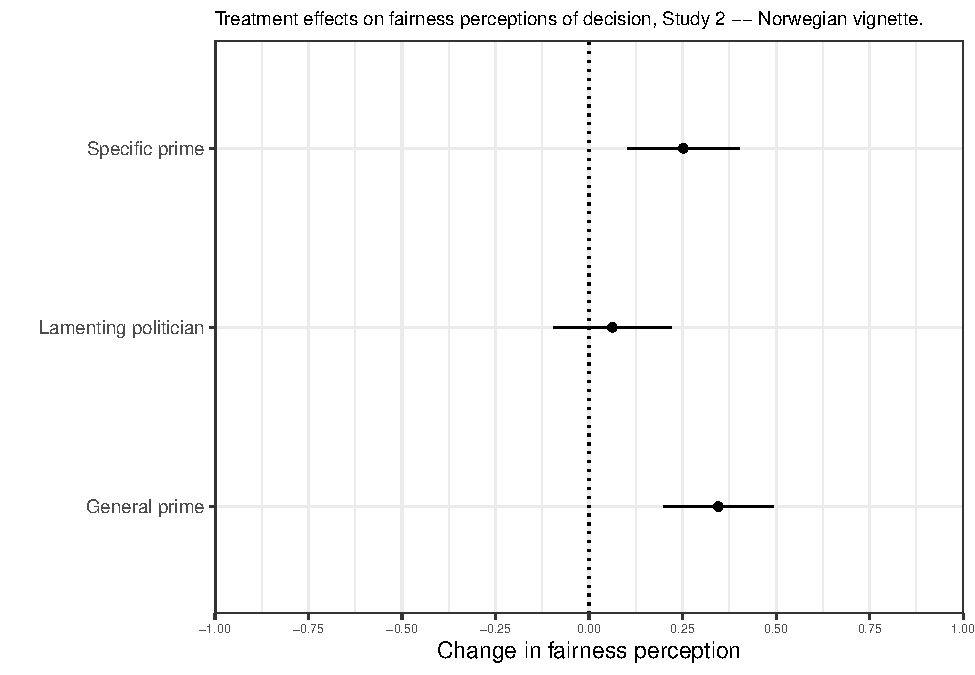
\includegraphics{Goodloser-appendix_files/figure-latex/204_post_fairness-1.pdf} \textbackslash begin\{table\}

\textbackslash caption\{(\#tab:204\_post\_fairness)Treatment effects on fairness perceptions of decision, Study 2 -- Norwegian vignette\}
\centering

\begin{tabular}[t]{lrrrr}
\toprule
Treatment value & Estimate & Std. Error & t-statistic & p value\\
\midrule
Not shown (Intercept) & 3.74 & 0.05 & 68.62 & 0.00\\
Lamenting politician & 0.06 & 0.08 & 0.80 & 0.43\\
General prime & 0.35 & 0.07 & 4.68 & 0.00\\
Specific prime & 0.25 & 0.07 & 3.38 & 0.00\\
\bottomrule
\end{tabular}

\textbackslash end\{table\}

\hypertarget{willingnes-to-accept}{%
\section{Willingnes to accept}\label{willingnes-to-accept}}

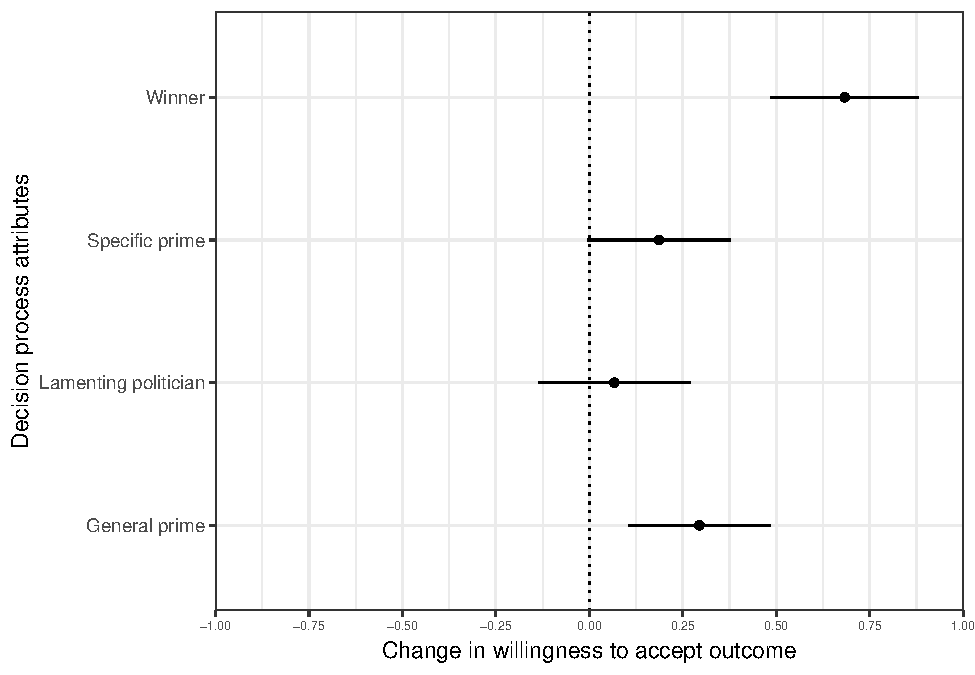
\includegraphics{Goodloser-appendix_files/figure-latex/204_post_accept-1.pdf} \textbackslash begin\{table\}

\textbackslash caption\{(\#tab:204\_post\_accept)Treatment effects on willingness to accept decision, Study 2 -- Norwegian vignette\}
\centering

\begin{tabular}[t]{lrrrr}
\toprule
Treatment value & Estimate & Std. Error & t-statistic & p value\\
\midrule
Not shown (Intercept) & 3.52 & 0.07 & 50.01 & 0.00\\
Lamenting politician & 0.07 & 0.10 & 0.66 & 0.51\\
General prime & 0.29 & 0.09 & 3.10 & 0.00\\
Specific prime & 0.19 & 0.10 & 1.95 & 0.05\\
\bottomrule
\end{tabular}

\textbackslash end\{table\}

\hypertarget{trust-in-politician}{%
\section{Trust in politician}\label{trust-in-politician}}

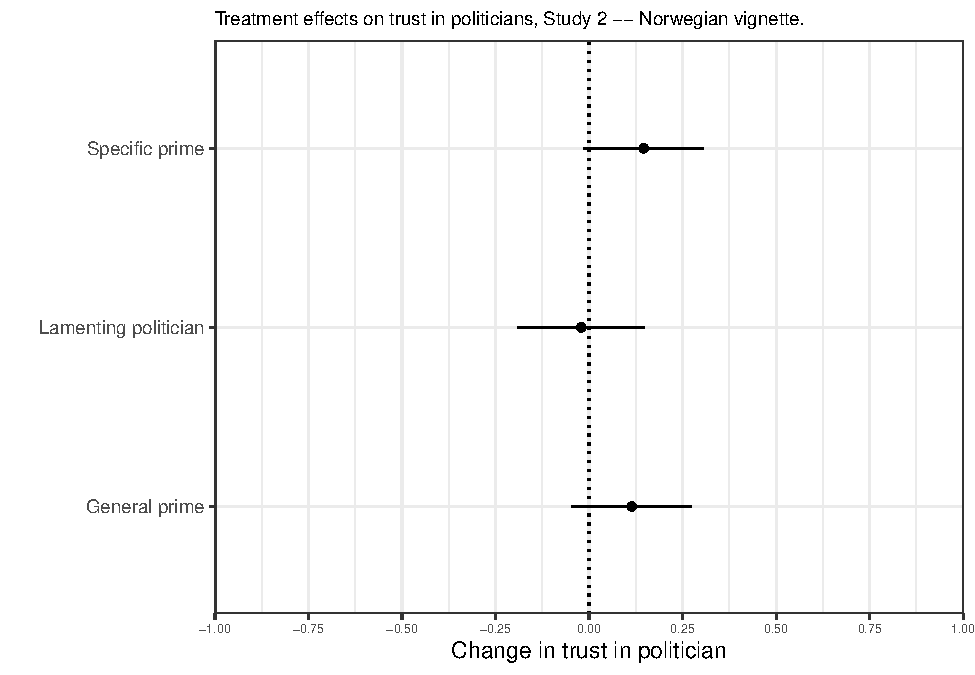
\includegraphics{Goodloser-appendix_files/figure-latex/204_post_trust-1.pdf} \textbackslash begin\{table\}

\textbackslash caption\{(\#tab:204\_post\_trust)Treatment effects on trust in politician, Study 2 -- Norwegian vignette\}
\centering

\begin{tabular}[t]{lrrrr}
\toprule
Treatment value & Estimate & Std. Error & t-statistic & p value\\
\midrule
Not shown (Intercept) & 3.23 & 0.06 & 54.50 & 0.00\\
Lamenting politician & -0.02 & 0.08 & -0.25 & 0.80\\
General prime & 0.11 & 0.08 & 1.42 & 0.16\\
Specific prime & 0.15 & 0.08 & 1.81 & 0.07\\
\bottomrule
\end{tabular}

\textbackslash end\{table\}

\hypertarget{main-effects-with-reduced-sample}{%
\chapter{Main effects with reduced sample}\label{main-effects-with-reduced-sample}}

\begin{quote}
Main effects with sample that excludes respondents who fail manipulation check
\end{quote}

\hypertarget{fairness-3}{%
\section{Fairness}\label{fairness-3}}

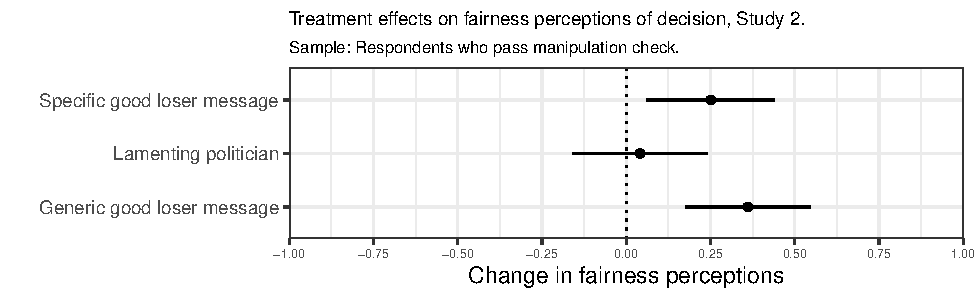
\includegraphics{Goodloser-appendix_files/figure-latex/2045_post_fairness-1.pdf} \textbackslash begin\{table\}

\textbackslash caption\{(\#tab:2045\_post\_fairness)Treatment effects on fairness perceptions of decision, Study 2 -- Norwegian vignette. Sample: Respondents who pass manipulation check\}
\centering

\begin{tabular}[t]{lrrrr}
\toprule
Treatment value & Estimate & Std. Error & t-statistic & p value\\
\midrule
Not shown (Intercept) & 3.76 & 0.07 & 56.49 & 0.00\\
Lamenting politician & 0.04 & 0.10 & 0.43 & 0.67\\
General prime & 0.36 & 0.09 & 4.09 & 0.00\\
Specific prime & 0.25 & 0.09 & 2.78 & 0.01\\
\bottomrule
\end{tabular}

\textbackslash end\{table\}

\hypertarget{willingnes-to-accept-1}{%
\section{Willingnes to accept}\label{willingnes-to-accept-1}}

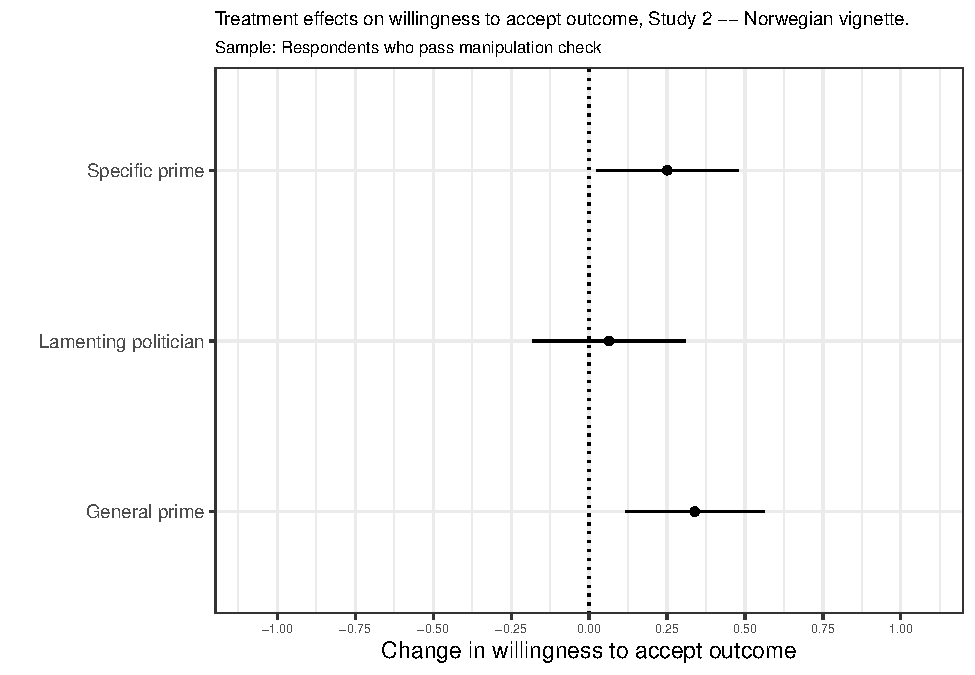
\includegraphics{Goodloser-appendix_files/figure-latex/2045_post_accept-1.pdf} \textbackslash begin\{table\}

\textbackslash caption\{(\#tab:2045\_post\_accept)Treatment effects on willingness to accept decision, Study 2 -- Norwegian vignette. Sample: Respondents who pass manipulation check.\}
\centering

\begin{tabular}[t]{lrrrr}
\toprule
Treatment value & Estimate & Std. Error & t-statistic & p value\\
\midrule
Not shown (Intercept) & 3.45 & 0.08 & 41.16 & 0.00\\
Lamenting politician & 0.06 & 0.12 & 0.51 & 0.61\\
General prime & 0.34 & 0.11 & 3.03 & 0.00\\
Specific prime & 0.25 & 0.11 & 2.20 & 0.03\\
\bottomrule
\end{tabular}

\textbackslash end\{table\}

\hypertarget{trust-in-politician-1}{%
\section{Trust in politician}\label{trust-in-politician-1}}

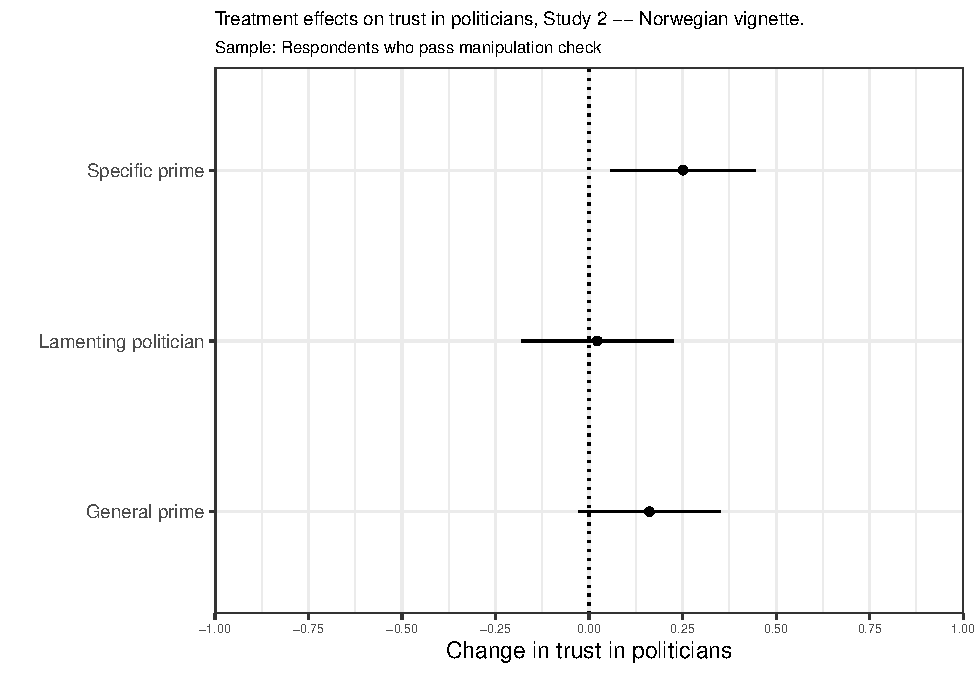
\includegraphics{Goodloser-appendix_files/figure-latex/2045_post_trust-1.pdf} \textbackslash begin\{table\}

\textbackslash caption\{(\#tab:2045\_post\_trust)Treatment effects on trust in politician, Study 2 -- Norwegian vignette. Sample: Respondents who pass manipulation check.\}
\centering

\begin{tabular}[t]{lrrrr}
\toprule
Treatment value & Estimate & Std. Error & t-statistic & p value\\
\midrule
Not shown (Intercept) & 3.17 & 0.07 & 44.36 & 0.00\\
Lamenting politician & 0.02 & 0.10 & 0.22 & 0.83\\
General prime & 0.16 & 0.09 & 1.71 & 0.09\\
Specific prime & 0.25 & 0.10 & 2.59 & 0.01\\
\bottomrule
\end{tabular}

\textbackslash end\{table\}

\hypertarget{main-effects-with-full-itt-sample}{%
\chapter{Main effects with full ITT sample}\label{main-effects-with-full-itt-sample}}

\hypertarget{fairness-4}{%
\section{Fairness}\label{fairness-4}}

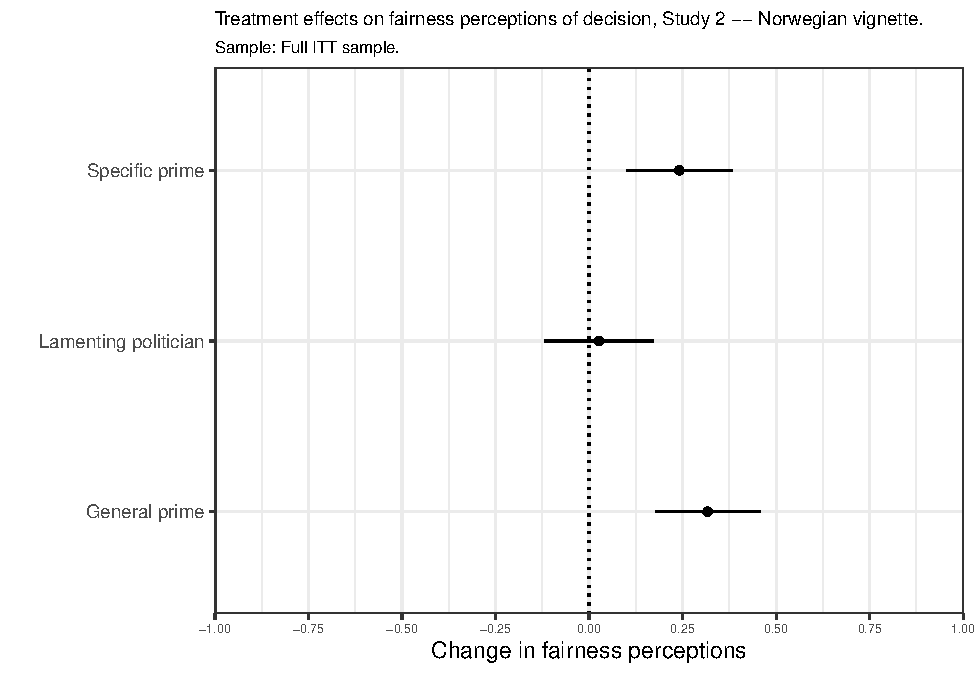
\includegraphics{Goodloser-appendix_files/figure-latex/2046_post_fairness-1.pdf} \textbackslash begin\{table\}

\textbackslash caption\{(\#tab:2046\_post\_fairness)Treatment effects on fairness perceptions of decision, Study 2 -- Norwegian vignette. `Sample: Full ITT sample.'\}
\centering

\begin{tabular}[t]{lrrrr}
\toprule
Treatment value & Estimate & Std. Error & t-statistic & p value\\
\midrule
Not shown (Intercept) & 3.74 & 0.05 & 72.52 & 0.00\\
Lamenting politician & 0.03 & 0.07 & 0.36 & 0.72\\
General prime & 0.32 & 0.07 & 4.51 & 0.00\\
Specific prime & 0.24 & 0.07 & 3.39 & 0.00\\
\bottomrule
\end{tabular}

\textbackslash end\{table\}

\hypertarget{willingnes-to-accept-2}{%
\section{Willingnes to accept}\label{willingnes-to-accept-2}}

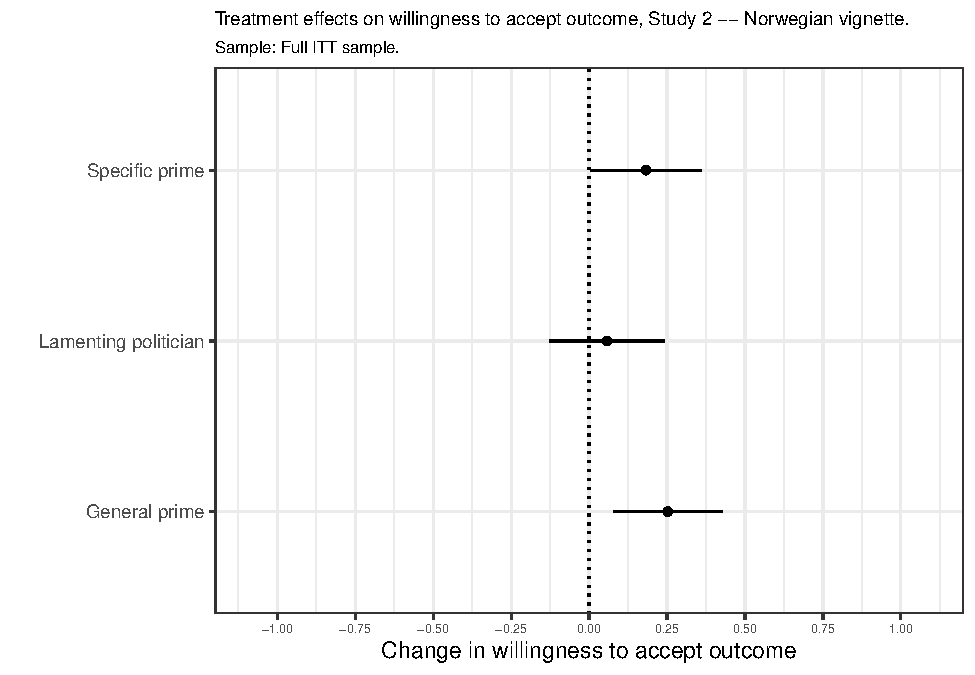
\includegraphics{Goodloser-appendix_files/figure-latex/2046_post_accept-1.pdf} \textbackslash begin\{table\}

\textbackslash caption\{(\#tab:2046\_post\_accept)Treatment effects on willingness to accept decision, Study 2 -- Norwegian vignette. Sample: Full ITT sample.\}
\centering

\begin{tabular}[t]{lrrrr}
\toprule
Treatment value & Estimate & Std. Error & t-statistic & p value\\
\midrule
Not shown (Intercept) & 3.53 & 0.06 & 54.45 & 0.00\\
Lamenting politician & 0.06 & 0.09 & 0.62 & 0.53\\
General prime & 0.25 & 0.09 & 2.88 & 0.00\\
Specific prime & 0.18 & 0.09 & 2.06 & 0.04\\
\bottomrule
\end{tabular}

\textbackslash end\{table\}

\hypertarget{trust-in-politician-2}{%
\section{Trust in politician}\label{trust-in-politician-2}}

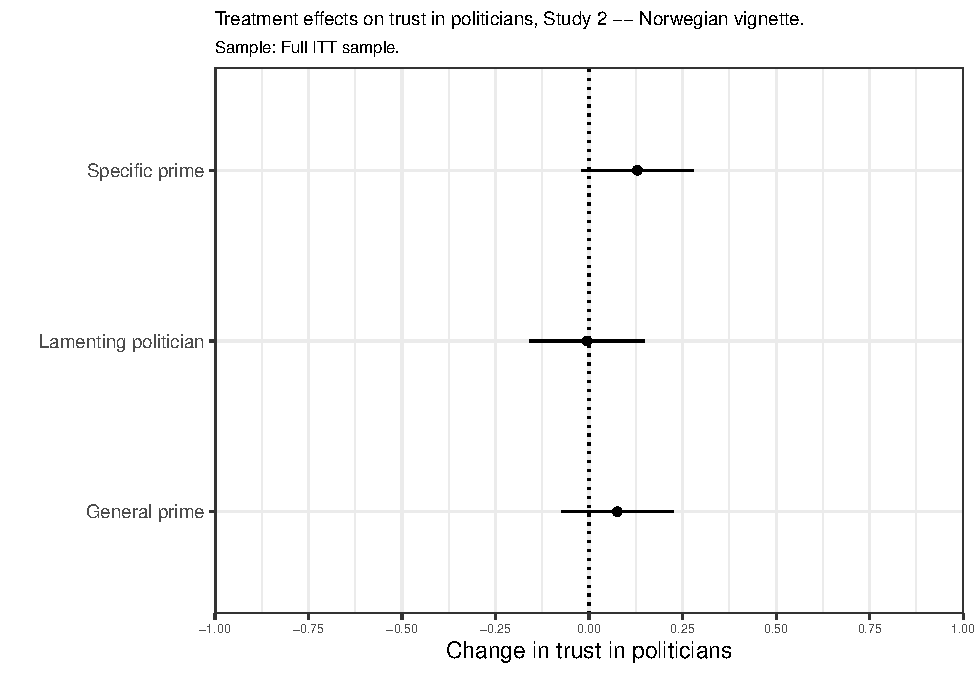
\includegraphics{Goodloser-appendix_files/figure-latex/2046_post_trust-1.pdf} \textbackslash begin\{table\}

\textbackslash caption\{(\#tab:2046\_post\_trust)Treatment effects on trust in politician, Study 2 -- Norwegian vignette. Sample: Full ITT sample.\}
\centering

\begin{tabular}[t]{lrrrr}
\toprule
Treatment value & Estimate & Std. Error & t-statistic & p value\\
\midrule
Not shown (Intercept) & 3.22 & 0.05 & 58.83 & 0.00\\
Lamenting politician & -0.01 & 0.08 & -0.08 & 0.94\\
General prime & 0.08 & 0.07 & 1.02 & 0.31\\
Specific prime & 0.13 & 0.08 & 1.72 & 0.09\\
\bottomrule
\end{tabular}

\textbackslash end\{table\}

\hypertarget{effects-on-losers-1}{%
\chapter{Effects on losers}\label{effects-on-losers-1}}

\begin{quote}
Main effects with ITT sample of respondents who receive an unfavorable outcome.
\end{quote}

\hypertarget{fairness-5}{%
\section{Fairness}\label{fairness-5}}

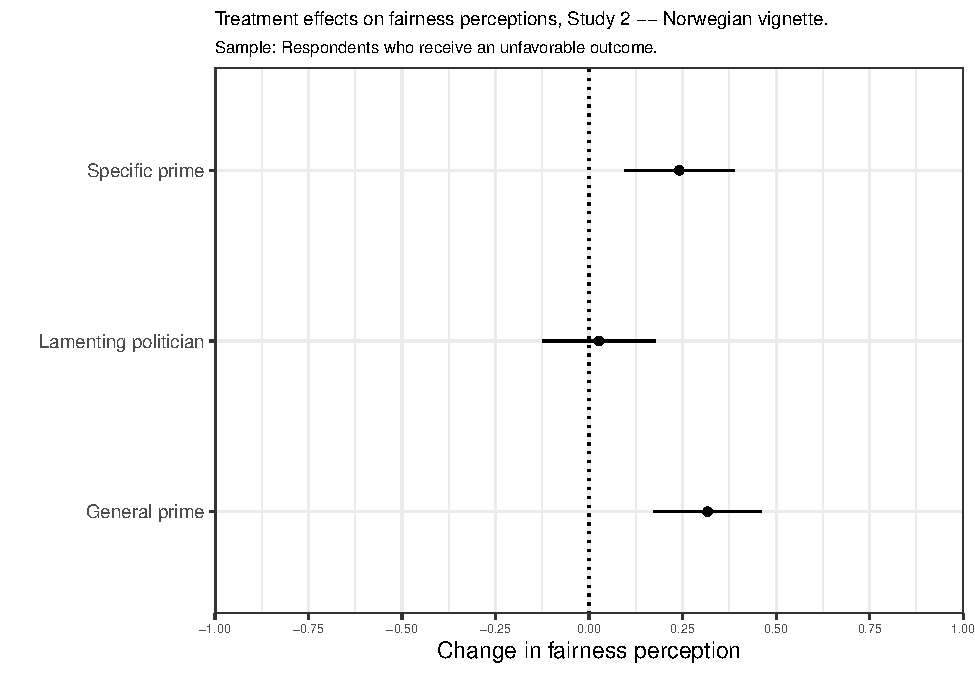
\includegraphics{Goodloser-appendix_files/figure-latex/205_post_fairness-1.pdf} \textbackslash begin\{table\}

\textbackslash caption\{(\#tab:205\_post\_fairness)Treatment effects among losers on fairness perceptions of decision, Study 2 -- Norwegian vignette\}
\centering

\begin{tabular}[t]{lrrrr}
\toprule
Treatment value & Estimate & Std. Error & t-statistic & p value\\
\midrule
Not shown (Intercept) & 3.74 & 0.05 & 70.22 & 0.00\\
Lamenting politician & 0.03 & 0.08 & 0.35 & 0.72\\
General prime & 0.32 & 0.07 & 4.37 & 0.00\\
Specific prime & 0.24 & 0.07 & 3.28 & 0.00\\
\bottomrule
\end{tabular}

\textbackslash end\{table\}
\#\#\# Fairness II
\textgreater{} Lamenting politician as reference category

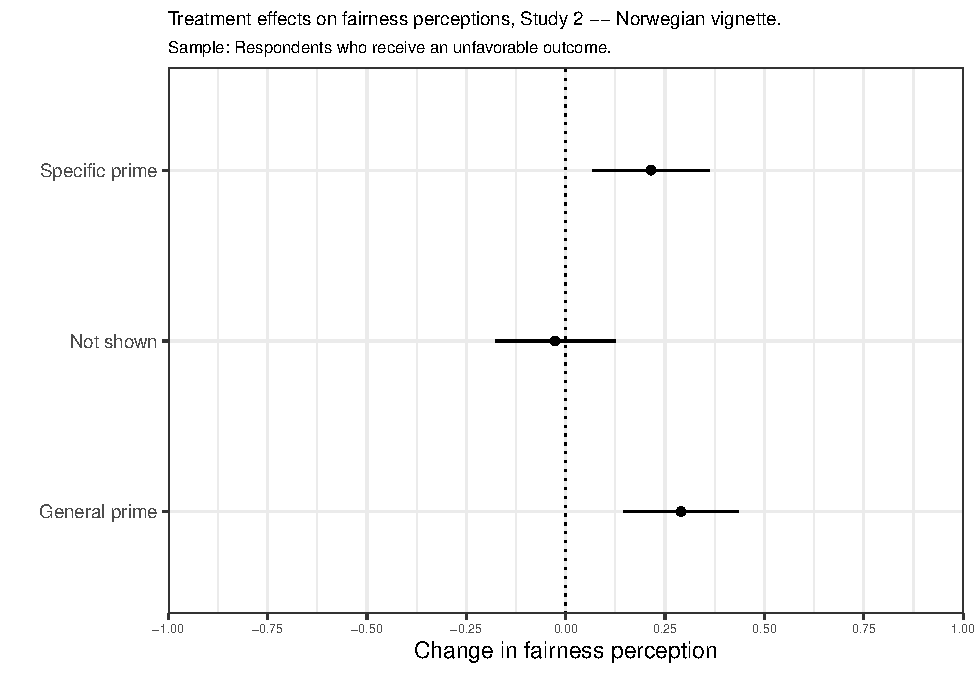
\includegraphics{Goodloser-appendix_files/figure-latex/2055_post_fairness-1.pdf} \textbackslash begin\{table\}

\textbackslash caption\{(\#tab:2055\_post\_fairness)Treatment effects among losers on fairness perceptions of decision, Study 2 -- Norwegian vignette\}
\centering

\begin{tabular}[t]{lrrrr}
\toprule
Treatment value & Estimate & Std. Error & t-statistic & p value\\
\midrule
Intercept & 3.77 & 0.05 & 70.55 & 0.00\\
General prime & 0.29 & 0.07 & 4.00 & 0.00\\
Not shown & -0.03 & 0.08 & -0.35 & 0.72\\
Specific prime & 0.21 & 0.07 & 2.92 & 0.00\\
\bottomrule
\end{tabular}

\textbackslash end\{table\}

\hypertarget{fairness-moderated-by-issue-importance}{%
\subsection{Fairness moderated by issue importance}\label{fairness-moderated-by-issue-importance}}

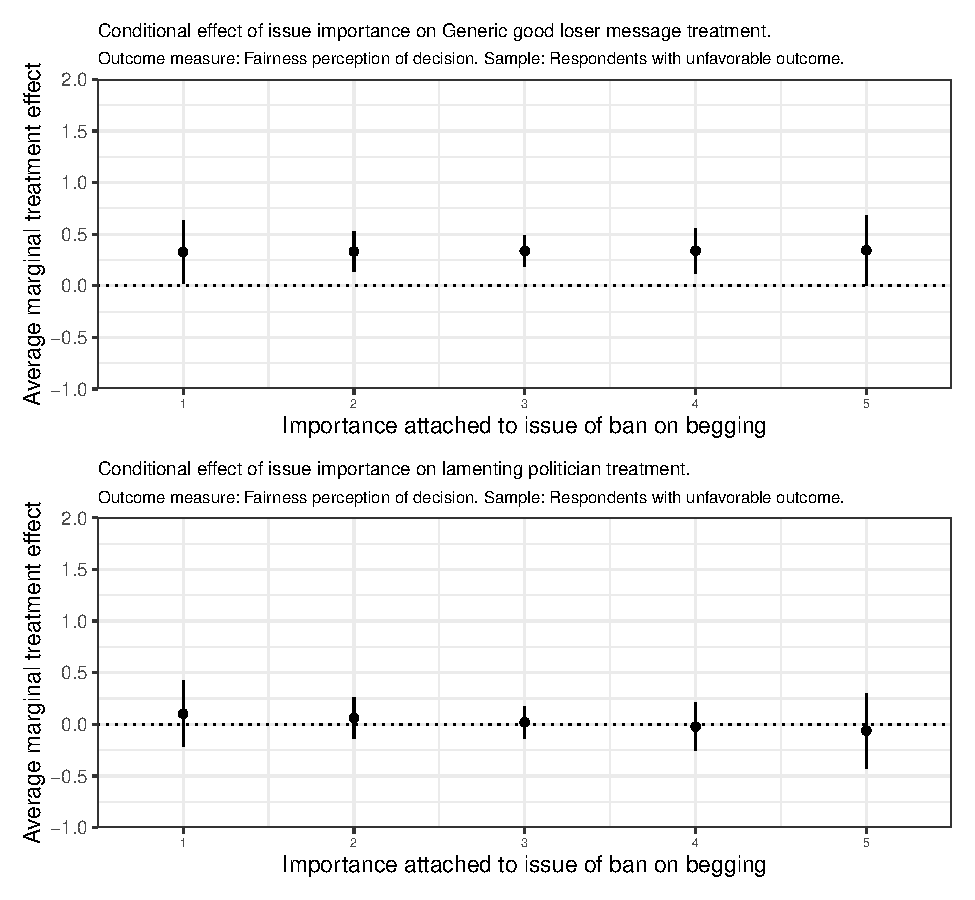
\includegraphics{Goodloser-appendix_files/figure-latex/2050_importance_treatment_fairness-1.pdf} 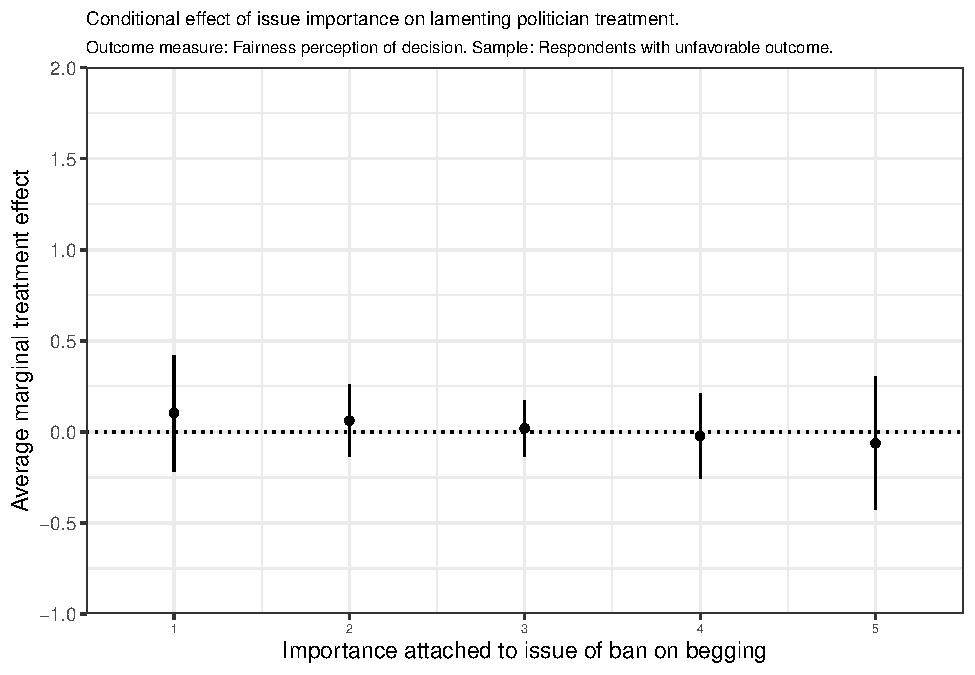
\includegraphics{Goodloser-appendix_files/figure-latex/2050_importance_treatment_fairness-2.pdf} \textbackslash begin\{table\}{[}H{]}

\textbackslash caption\{(\#tab:2050\_importance\_treatment\_fairness)Moderating effects of issue importance on experimental treatment, Study 2 -- Norwegian vignette\}
\centering

\begin{tabular}[t]{lrrrrrrr}
\toprule
Factor & Issue importance & AME & SE & z-statistic & p value & Lower & Upper\\
\midrule
General prime & 1 & 0.33 & 0.15 & 2.13 & 0.03 & 0.03 & 0.63\\
General prime & 2 & 0.33 & 0.10 & 3.42 & 0.00 & 0.14 & 0.52\\
General prime & 3 & 0.34 & 0.07 & 4.56 & 0.00 & 0.19 & 0.48\\
General prime & 4 & 0.34 & 0.11 & 3.13 & 0.00 & 0.13 & 0.55\\
General prime & 5 & 0.34 & 0.17 & 2.04 & 0.04 & 0.01 & 0.67\\
\addlinespace
Lamenting politician & 1 & 0.10 & 0.16 & 0.65 & 0.52 & -0.21 & 0.41\\
Lamenting politician & 2 & 0.06 & 0.10 & 0.62 & 0.53 & -0.13 & 0.25\\
Lamenting politician & 3 & 0.02 & 0.08 & 0.26 & 0.80 & -0.13 & 0.17\\
Lamenting politician & 4 & -0.02 & 0.12 & -0.18 & 0.86 & -0.25 & 0.21\\
Lamenting politician & 5 & -0.06 & 0.18 & -0.34 & 0.73 & -0.42 & 0.30\\
\bottomrule
\multicolumn{8}{l}{\textit{Note: }}\\
\multicolumn{8}{l}{Sample: Respondents with unfavorable outcome.}\\
\end{tabular}

\textbackslash end\{table\}
\#\#\# Fairness moderated by good loser norm
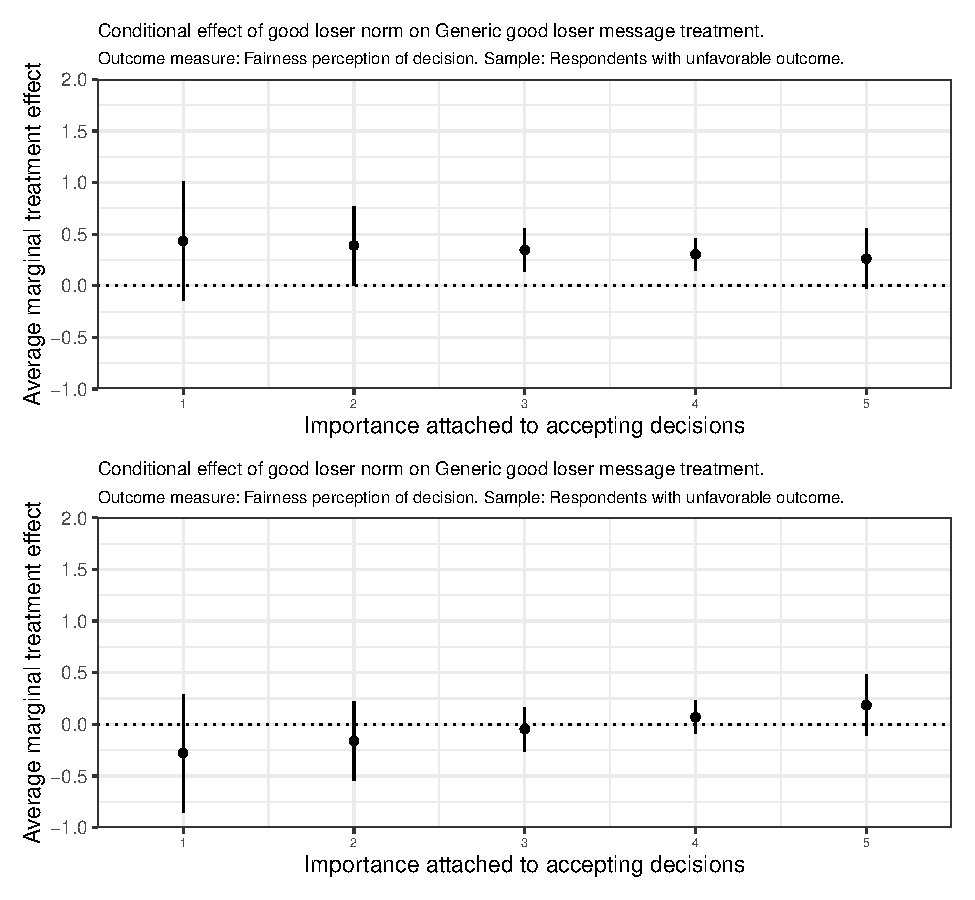
\includegraphics{Goodloser-appendix_files/figure-latex/2050_norm_treatment_fairness-1.pdf} 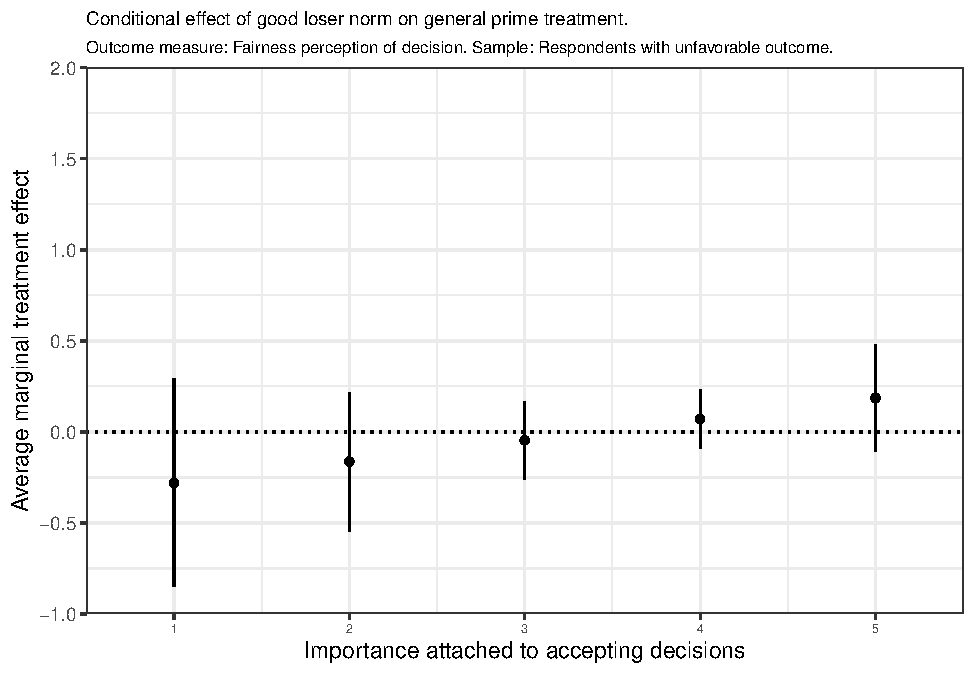
\includegraphics{Goodloser-appendix_files/figure-latex/2050_norm_treatment_fairness-2.pdf} \textbackslash begin\{table\}{[}H{]}

\textbackslash caption\{(\#tab:2050\_norm\_treatment\_fairness)Moderating effects of norm importance on experimental treatment, Study 2 -- Norwegian vignette\}
\centering

\begin{tabular}[t]{lrrrrrrr}
\toprule
Factor & Norm importance & AME & SE & z-statistic & p value & Lower & Upper\\
\midrule
General prime & 1 & 0.43 & 0.29 & 1.50 & 0.13 & -0.13 & 1.00\\
General prime & 2 & 0.39 & 0.19 & 2.03 & 0.04 & 0.01 & 0.76\\
General prime & 3 & 0.35 & 0.11 & 3.29 & 0.00 & 0.14 & 0.55\\
General prime & 4 & 0.30 & 0.08 & 3.91 & 0.00 & 0.15 & 0.46\\
General prime & 5 & 0.26 & 0.15 & 1.79 & 0.07 & -0.03 & 0.55\\
\addlinespace
Lamenting politician & 1 & -0.28 & 0.29 & -0.98 & 0.33 & -0.84 & 0.28\\
Lamenting politician & 2 & -0.16 & 0.19 & -0.85 & 0.39 & -0.54 & 0.21\\
Lamenting politician & 3 & -0.05 & 0.11 & -0.43 & 0.66 & -0.26 & 0.16\\
Lamenting politician & 4 & 0.07 & 0.08 & 0.87 & 0.39 & -0.09 & 0.23\\
Lamenting politician & 5 & 0.19 & 0.15 & 1.26 & 0.21 & -0.10 & 0.48\\
\bottomrule
\multicolumn{8}{l}{\textit{Note: }}\\
\multicolumn{8}{l}{Sample: Respondents with unfavorable outcome.}\\
\end{tabular}

\textbackslash end\{table\}

\hypertarget{willingnes-to-accept-3}{%
\section{Willingnes to accept}\label{willingnes-to-accept-3}}

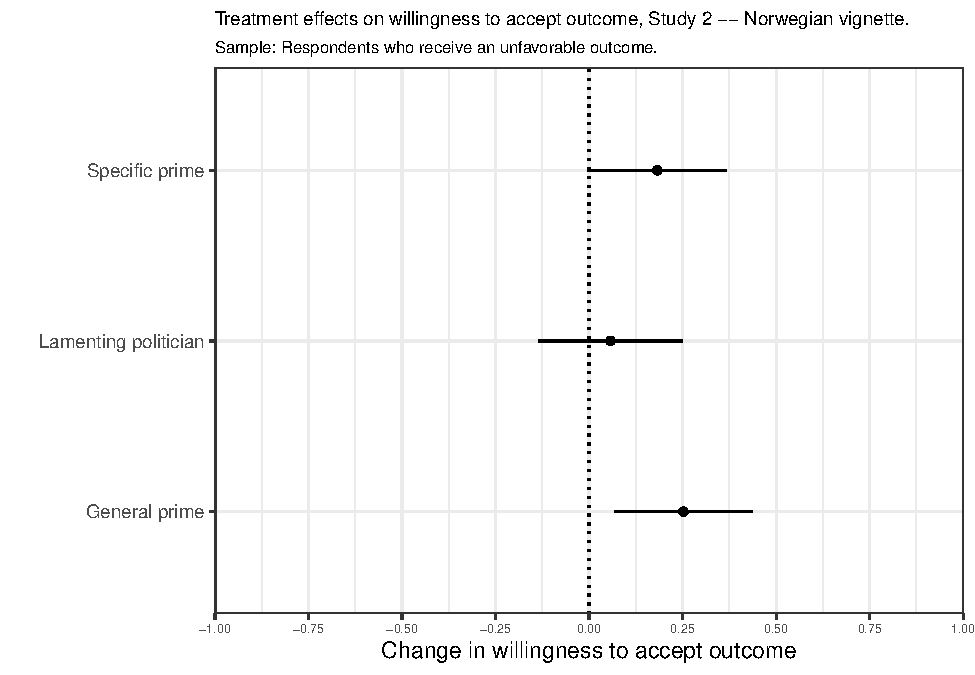
\includegraphics{Goodloser-appendix_files/figure-latex/205_post_accept-1.pdf} \textbackslash begin\{table\}

\textbackslash caption\{(\#tab:205\_post\_accept)Treatment effects among losers on willingness to accept decision, Study 2 -- Norwegian vignette\}
\centering

\begin{tabular}[t]{lrrrr}
\toprule
Treatment value & Estimate & Std. Error & t-statistic & p value\\
\midrule
Not shown (Intercept) & 3.53 & 0.07 & 51.98 & 0.00\\
Lamenting politician & 0.06 & 0.10 & 0.60 & 0.55\\
General prime & 0.25 & 0.09 & 2.74 & 0.01\\
Specific prime & 0.18 & 0.09 & 1.96 & 0.05\\
\bottomrule
\end{tabular}

\textbackslash end\{table\}

\hypertarget{trust-in-politician-3}{%
\section{Trust in politician}\label{trust-in-politician-3}}

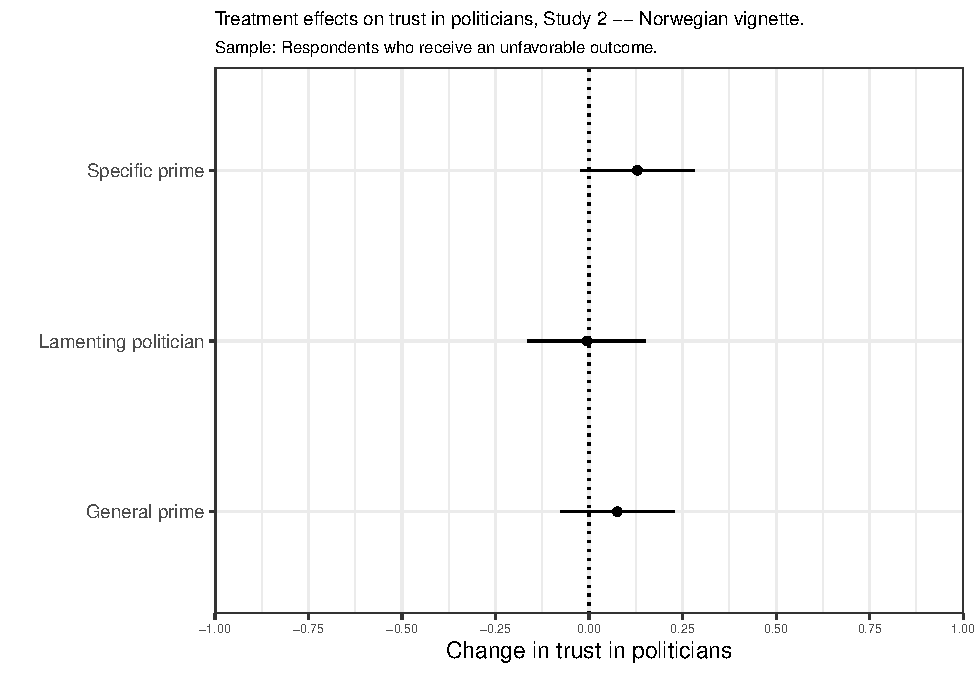
\includegraphics{Goodloser-appendix_files/figure-latex/205_post_trust-1.pdf} \textbackslash begin\{table\}

\textbackslash caption\{(\#tab:205\_post\_trust)Treatment effects among losers on trust in politician, Study 2 -- Norwegian vignette\}
\centering

\begin{tabular}[t]{lrrrr}
\toprule
Treatment value & Estimate & Std. Error & t-statistic & p value\\
\midrule
Not shown (Intercept) & 3.22 & 0.06 & 57.66 & 0.00\\
Lamenting politician & -0.01 & 0.08 & -0.07 & 0.94\\
General prime & 0.08 & 0.08 & 1.00 & 0.32\\
Specific prime & 0.13 & 0.08 & 1.68 & 0.09\\
\bottomrule
\end{tabular}

\textbackslash end\{table\}

\hypertarget{codebook-1}{%
\chapter{Codebook}\label{codebook-1}}

\begin{quote}
This chapter displays the codebook for the data set of the first Good Loser experiment, generated using the R package ``codebook''.
\end{quote}

\begin{verbatim}
## # A tibble: 17,011 x 30
##    responseid   r9pad1   r9pad2   r9pad3 r10panelpad  r10pad1  r10pad2
##         <dbl> <dbl+lb> <dbl+lb> <dbl+lb>   <dbl+lbl> <dbl+lb> <dbl+lb>
##  1         NA NA       NA       NA       NA          NA       NA      
##  2    1000001 NA       NA       NA        0 [Histor~ 98 [Not~ 98 [Not~
##  3    1000002 NA       NA       NA        0 [Histor~ 98 [Not~ 98 [Not~
##  4    1000003 NA       NA       NA       NA          NA       NA      
##  5    1000004 NA       NA       NA       NA          NA       NA      
##  6    1000005 NA       NA       NA       NA          NA       NA      
##  7    1000006 NA       NA       NA       NA          NA       NA      
##  8    1000007 98 [Not~ 98 [Not~ 98 [Not~ NA          NA       NA      
##  9    1000008 NA       NA       NA       NA          NA       NA      
## 10    1000009 NA       NA       NA       NA          NA       NA      
## # ... with 17,001 more rows, and 23 more variables: r10pad3_mobil <dbl+lbl>,
## #   r10pad3a_ran <dbl+lbl>, r10pad3b_ran <dbl+lbl>, r10pad3ended <dbl>,
## #   r10pad3error <dbl>, r10pad3paused <dbl>, r10pad3played <dbl>,
## #   r10pad3_timespent <dbl>, r10pad4 <dbl+lbl>, r10pad4_comment <chr>,
## #   r10pad5 <dbl+lbl>, r10pad6 <dbl+lbl>, r10pad7 <dbl+lbl>, r10pad8 <dbl+lbl>,
## #   r10pad9 <dbl+lbl>, r10pad1_9_backward_1 <dbl+lbl>,
## #   r10pad1_9_backward_2 <dbl+lbl>, r10pad1_9_backward_3 <dbl+lbl>,
## #   r10pad1_9_backward_4 <dbl+lbl>, r10pad1_9_backward_5 <dbl+lbl>,
## #   r10pad1_9_backward_6 <dbl+lbl>, r10pad1_9_backward_7 <dbl+lbl>,
## #   r10pad1_9_backward_8 <dbl+lbl>
\end{verbatim}

\hypertarget{metadata-1}{%
\subsection{Metadata}\label{metadata-1}}

\hypertarget{description-1}{%
\subsubsection{Description}\label{description-1}}

\textbf{Dataset name}: d

The dataset has N=17011 rows and 30 columns.
0 rows have no missing values on any column.

Metadata for search engines

\begin{itemize}
\item
  \textbf{Date published}: 2020-04-17

  \begin{itemize}
  \tightlist
  \item
    \textbf{keywords}: \emph{responseid}, \emph{r9pad1}, \emph{r9pad2}, \emph{r9pad3}, \emph{r10panelpad}, \emph{r10pad1}, \emph{r10pad2}, \emph{r10pad3\_mobil}, \emph{r10pad3a\_ran}, \emph{r10pad3b\_ran}, \emph{r10pad3ended}, \emph{r10pad3error}, \emph{r10pad3paused}, \emph{r10pad3played}, \emph{r10pad3\_timespent}, \emph{r10pad4}, \emph{r10pad4\_comment}, \emph{r10pad5}, \emph{r10pad6}, \emph{r10pad7}, \emph{r10pad8}, \emph{r10pad9}, \emph{r10pad1\_9\_backward\_1}, \emph{r10pad1\_9\_backward\_2}, \emph{r10pad1\_9\_backward\_3}, \emph{r10pad1\_9\_backward\_4}, \emph{r10pad1\_9\_backward\_5}, \emph{r10pad1\_9\_backward\_6}, \emph{r10pad1\_9\_backward\_7} and \emph{r10pad1\_9\_backward\_8}
  \end{itemize}
\end{itemize}

\hypertarget{variables-1}{%
\section{Variables}\label{variables-1}}

\hypertarget{Q64}{%
\subsection{Q64}\label{Q64}}

Ålder

\hypertarget{Q64_distribution}{%
\subsubsection{Distribution}\label{Q64_distribution}}

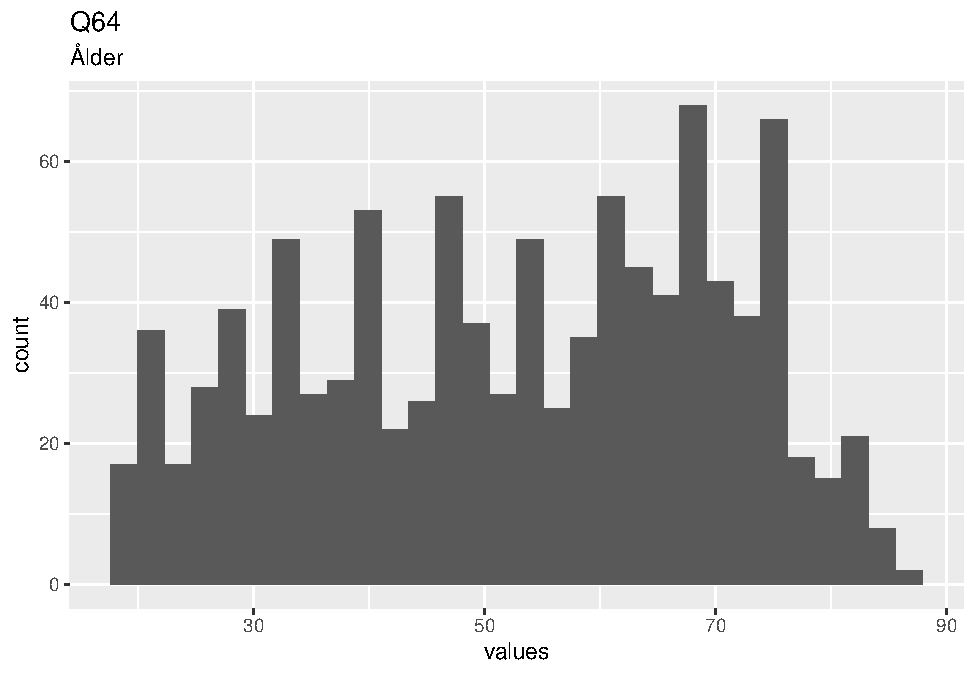
\includegraphics{Goodloser-appendix_files/figure-latex/cb_d_Q64_distribution-1.pdf}

4 missing values.

\hypertarget{Q64_summary}{%
\subsubsection{Summary statistics}\label{Q64_summary}}

\begin{tabular}{l|l|l|r|r|l|l|l|r|r|l|l|l}
\hline
name & label & data_type & n_missing & complete_rate & min & median & max & mean & sd & hist & format.spss & display_width\\
\hline
Q64 & Ålder & numeric & 4 & 0.9961 & 18 & 54 & 86 & 52.46 & 17.74 & ▅▆▆▇▃ & F8.0 & 10\\
\hline
\end{tabular}

\hypertarget{Q63}{%
\subsection{Q63}\label{Q63}}

Kön

\hypertarget{Q63_distribution}{%
\subsubsection{Distribution}\label{Q63_distribution}}

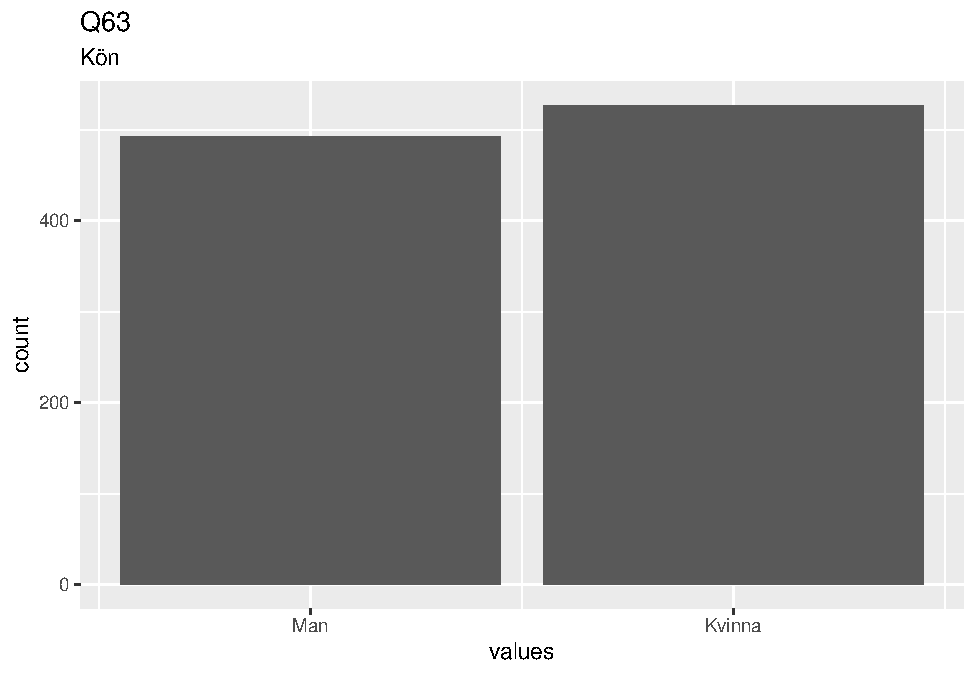
\includegraphics{Goodloser-appendix_files/figure-latex/cb_d_Q63_distribution-1.pdf}

0 missing values.

\hypertarget{Q63_summary}{%
\subsubsection{Summary statistics}\label{Q63_summary}}

\begin{tabular}{l|l|l|l|r|r|l|l|l|r|r|r|l|l|l}
\hline
name & label & data_type & value_labels & n_missing & complete_rate & min & median & max & mean & sd & n_value_labels & hist & format.spss & display_width\\
\hline
Q63 & Kön & haven_labelled & 1. Man,<br>2. Kvinna & 0 & 1 & 1 & 2 & 2 & 1.517 & 0.5 & 2 & ▇▁▁▁▁▁▁▇ & F1.0 & 12\\
\hline
\end{tabular}

\hypertarget{Q63_labels}{%
\subsubsection{Value labels}\label{Q63_labels}}

\begin{itemize}
\tightlist
\item
  \textbf{Man}: \emph{1}
\item
  \textbf{Kvinna}: \emph{2}
\end{itemize}

\hypertarget{S3_1_1}{%
\subsection{S3\_1\_1}\label{S3_1_1}}

I debatten diskuteras ibland att kommunerna skall kunna förbjuda tiggeri inom sina gränser. Vad tycker du själv om att förbjuda tiggeri i kommunen där du bor?

\hypertarget{S3_1_1_distribution}{%
\subsubsection{Distribution}\label{S3_1_1_distribution}}

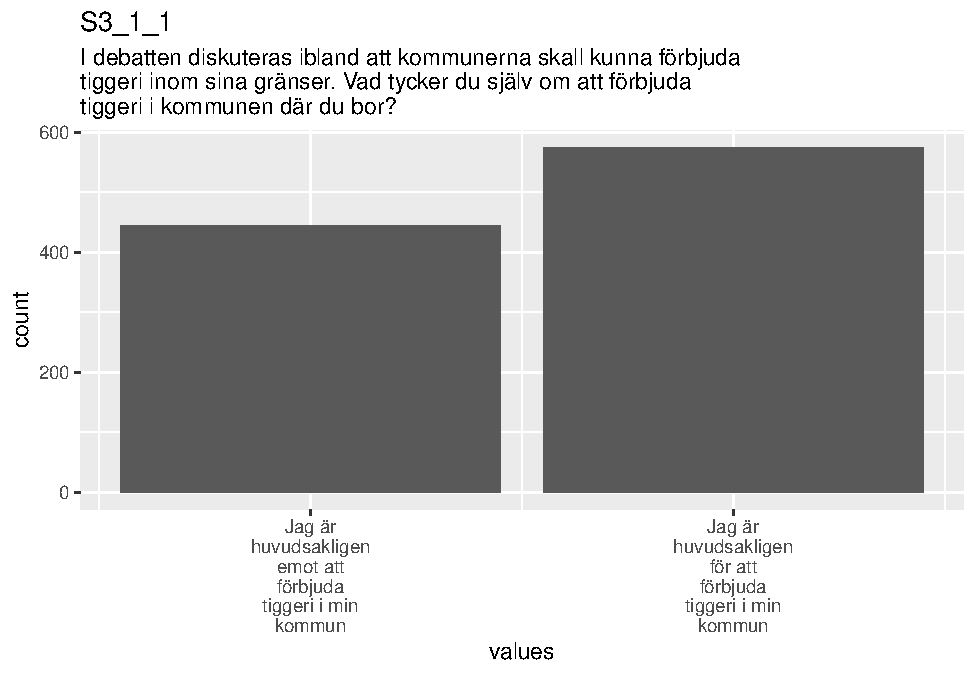
\includegraphics{Goodloser-appendix_files/figure-latex/cb_d_S3_1_1_distribution-1.pdf}

0 missing values.

\hypertarget{S3_1_1_summary}{%
\subsubsection{Summary statistics}\label{S3_1_1_summary}}

\begin{tabular}{l|l|l|l|r|r|l|l|l|r|r|r|l|l|l}
\hline
name & label & data_type & value_labels & n_missing & complete_rate & min & median & max & mean & sd & n_value_labels & hist & format.spss & display_width\\
\hline
S3_1_1 & I debatten diskuteras ibland att kommunerna skall kunna förbjuda tiggeri inom sina gränser. Vad tycker du själv om att förbjuda tiggeri i kommunen där du bor? & haven_labelled & 1. Jag är huvudsakligen emot att förbjuda tiggeri i min kommun,<br>2. Jag är huvudsakligen för att förbjuda tiggeri i min kommun & 0 & 1 & 1 & 2 & 2 & 1.563 & 0.4962 & 2 & ▆▁▁▁▁▁▁▇ & F1.0 & 12\\
\hline
\end{tabular}

\hypertarget{S3_1_1_labels}{%
\subsubsection{Value labels}\label{S3_1_1_labels}}

\begin{itemize}
\tightlist
\item
  \textbf{Jag är huvudsakligen emot att förbjuda tiggeri i min kommun}: \emph{1}
\item
  \textbf{Jag är huvudsakligen för att förbjuda tiggeri i min kommun}: \emph{2}
\end{itemize}

\hypertarget{S3_2_1}{%
\subsection{S3\_2\_1}\label{S3_2_1}}

Hur viktig är frågan för dig personligen?

\hypertarget{S3_2_1_distribution}{%
\subsubsection{Distribution}\label{S3_2_1_distribution}}

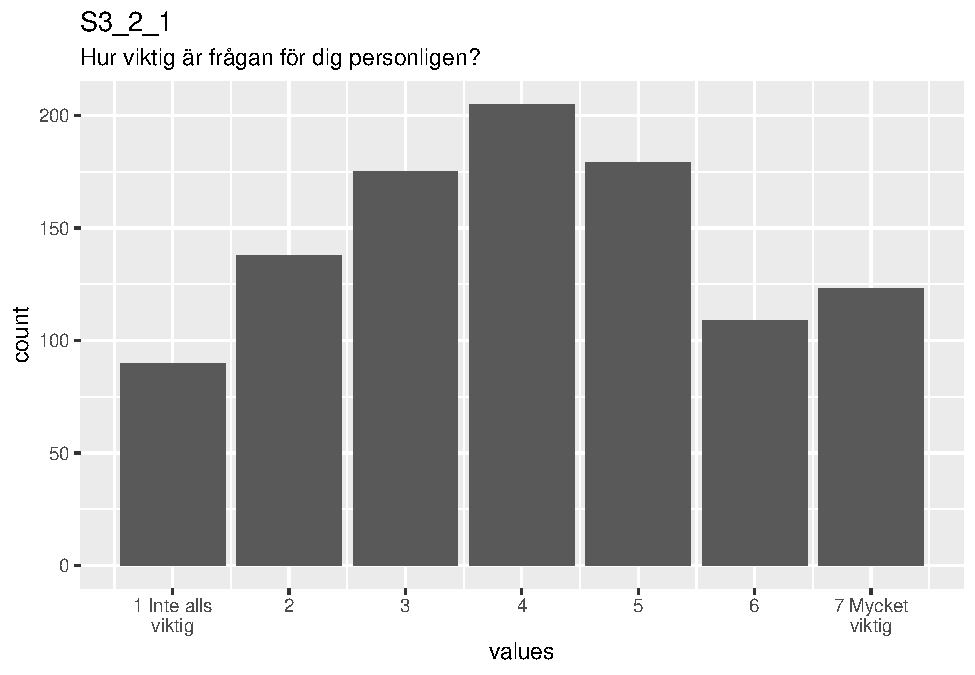
\includegraphics{Goodloser-appendix_files/figure-latex/cb_d_S3_2_1_distribution-1.pdf}

0 missing values.

\hypertarget{S3_2_1_summary}{%
\subsubsection{Summary statistics}\label{S3_2_1_summary}}

\begin{tabular}{l|l|l|l|r|r|l|l|l|r|r|r|l|l|l}
\hline
name & label & data_type & value_labels & n_missing & complete_rate & min & median & max & mean & sd & n_value_labels & hist & format.spss & display_width\\
\hline
S3_2_1 & Hur viktig är frågan för dig personligen? & haven_labelled & 1. 1 Inte alls viktig,<br>2. 2,<br>3. 3,<br>4. 4,<br>5. 5,<br>6. 6,<br>7. 7 Mycket viktig & 0 & 1 & 1 & 4 & 7 & 4.044 & 1.789 & 7 & ▃▆▇▇▁▇▅▅ & F1.0 & 12\\
\hline
\end{tabular}

\hypertarget{S3_2_1_labels}{%
\subsubsection{Value labels}\label{S3_2_1_labels}}

\begin{itemize}
\tightlist
\item
  \textbf{1 Inte alls viktig}: \emph{1}
\item
  \textbf{2}: \emph{2}
\item
  \textbf{3}: \emph{3}
\item
  \textbf{4}: \emph{4}
\item
  \textbf{5}: \emph{5}
\item
  \textbf{6}: \emph{6}
\item
  \textbf{7 Mycket viktig}: \emph{7}
\end{itemize}

\hypertarget{S3_4_1_1}{%
\subsection{S3\_4\_1\_1}\label{S3_4_1_1}}

Hur rättvist tycker du att det gick till när det fattades beslut om att förbjuda tiggeri?

\hypertarget{S3_4_1_1_distribution}{%
\subsubsection{Distribution}\label{S3_4_1_1_distribution}}

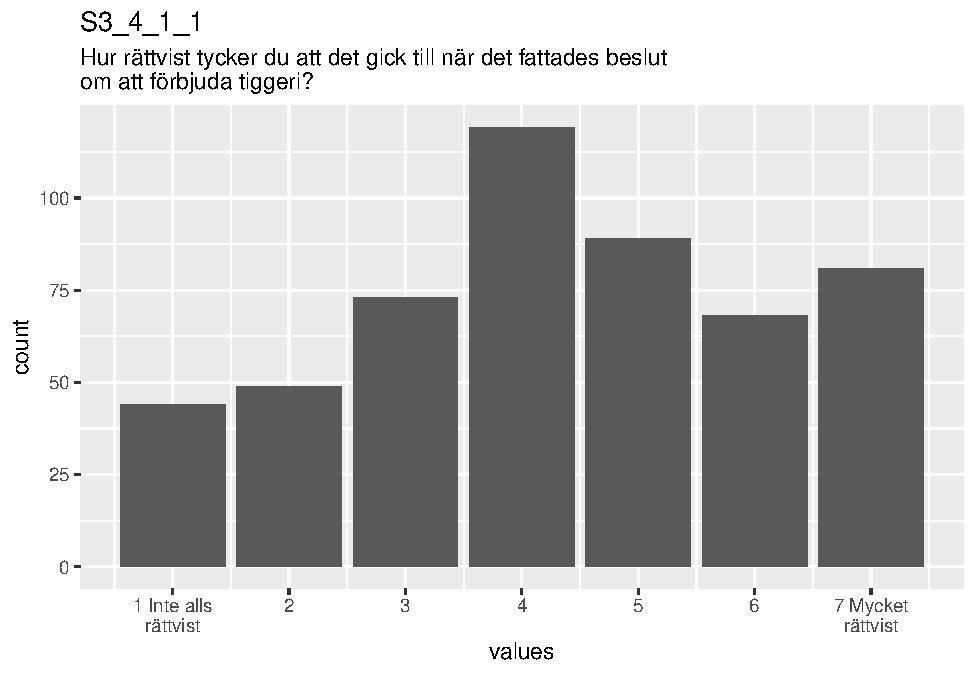
\includegraphics{Goodloser-appendix_files/figure-latex/cb_d_S3_4_1_1_distribution-1.pdf}

496 missing values.

\hypertarget{S3_4_1_1_summary}{%
\subsubsection{Summary statistics}\label{S3_4_1_1_summary}}

\begin{tabular}{l|l|l|l|r|r|l|l|l|r|r|r|l|l|l}
\hline
name & label & data_type & value_labels & n_missing & complete_rate & min & median & max & mean & sd & n_value_labels & hist & format.spss & display_width\\
\hline
S3_4_1_1 & Hur rättvist tycker du att det gick till när det fattades beslut om att förbjuda tiggeri? & haven_labelled & 1. 1 Inte alls rättvist,<br>2. 2,<br>3. 3,<br>4. 4,<br>5. 5,<br>6. 6,<br>7. 7 Mycket rättvist & 496 & 0.5132 & 1 & 4 & 7 & 4.316 & 1.806 & 7 & ▃▃▅▇▁▆▅▆ & F1.0 & 12\\
\hline
\end{tabular}

\hypertarget{S3_4_1_1_labels}{%
\subsubsection{Value labels}\label{S3_4_1_1_labels}}

\begin{itemize}
\tightlist
\item
  \textbf{1 Inte alls rättvist}: \emph{1}
\item
  \textbf{2}: \emph{2}
\item
  \textbf{3}: \emph{3}
\item
  \textbf{4}: \emph{4}
\item
  \textbf{5}: \emph{5}
\item
  \textbf{6}: \emph{6}
\item
  \textbf{7 Mycket rättvist}: \emph{7}
\end{itemize}

\hypertarget{S3_4_1_2}{%
\subsection{S3\_4\_1\_2}\label{S3_4_1_2}}

Hur rättvist tycker du att det gick till när det fattades beslut om att inte förbjuda tiggeri?

\hypertarget{S3_4_1_2_distribution}{%
\subsubsection{Distribution}\label{S3_4_1_2_distribution}}

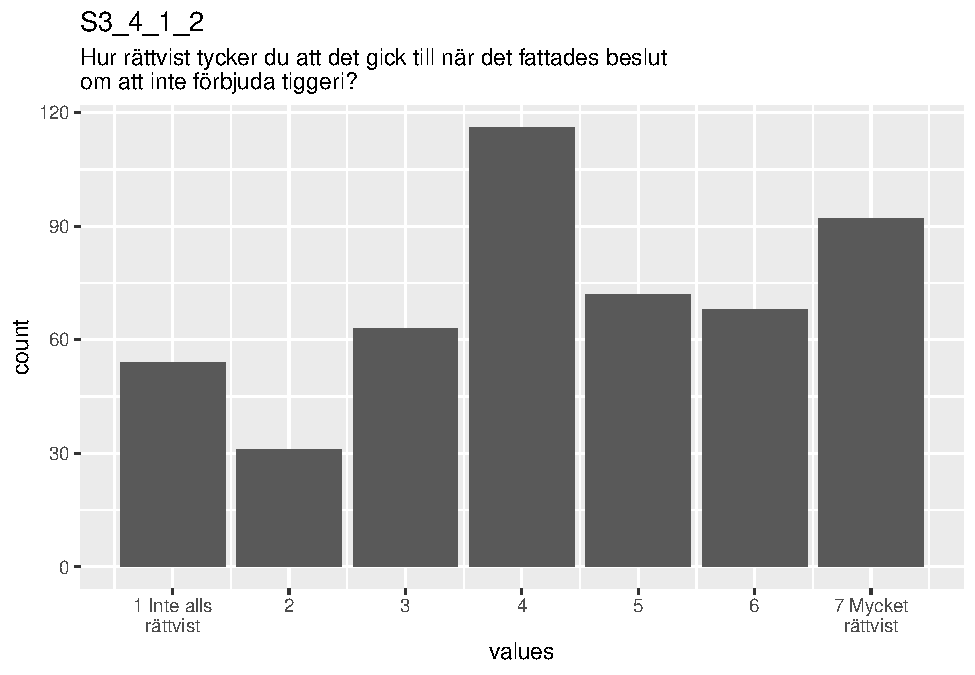
\includegraphics{Goodloser-appendix_files/figure-latex/cb_d_S3_4_1_2_distribution-1.pdf}

523 missing values.

\hypertarget{S3_4_1_2_summary}{%
\subsubsection{Summary statistics}\label{S3_4_1_2_summary}}

\begin{tabular}{l|l|l|l|r|r|l|l|l|r|r|r|l|l}
\hline
name & label & data_type & value_labels & n_missing & complete_rate & min & median & max & mean & sd & n_value_labels & hist & format.spss\\
\hline
S3_4_1_2 & Hur rättvist tycker du att det gick till när det fattades beslut om att inte förbjuda tiggeri? & haven_labelled & 1. 1 Inte alls rättvist,<br>2. 2,<br>3. 3,<br>4. 4,<br>5. 5,<br>6. 6,<br>7. 7 Mycket rättvist & 523 & 0.4868 & 1 & 4 & 7 & 4.397 & 1.889 & 7 & ▃▂▅▇▁▅▅▆ & F1.0\\
\hline
\end{tabular}

\hypertarget{S3_4_1_2_labels}{%
\subsubsection{Value labels}\label{S3_4_1_2_labels}}

\begin{itemize}
\tightlist
\item
  \textbf{1 Inte alls rättvist}: \emph{1}
\item
  \textbf{2}: \emph{2}
\item
  \textbf{3}: \emph{3}
\item
  \textbf{4}: \emph{4}
\item
  \textbf{5}: \emph{5}
\item
  \textbf{6}: \emph{6}
\item
  \textbf{7 Mycket rättvist}: \emph{7}
\end{itemize}

\hypertarget{S3_5_1}{%
\subsection{S3\_5\_1}\label{S3_5_1}}

Och hur schysst tycker du att beslutsproceduren var?

\hypertarget{S3_5_1_distribution}{%
\subsubsection{Distribution}\label{S3_5_1_distribution}}

\includegraphics{Goodloser-appendix_files/figure-latex/cb_d_S3_5_1_distribution-1.pdf}

0 missing values.

\hypertarget{S3_5_1_summary}{%
\subsubsection{Summary statistics}\label{S3_5_1_summary}}

\begin{tabular}{l|l|l|l|r|r|l|l|l|r|r|r|l|l|l}
\hline
name & label & data_type & value_labels & n_missing & complete_rate & min & median & max & mean & sd & n_value_labels & hist & format.spss & display_width\\
\hline
S3_5_1 & Och hur schysst tycker du att beslutsproceduren var? & haven_labelled & 1. 1 Mycket oschysst,<br>2. 2,<br>3. 3,<br>4. 4,<br>5. 5,<br>6. 6,<br>7. 7 Mycket schysst & 0 & 1 & 1 & 4 & 7 & 4.21 & 1.706 & 7 & ▂▂▅▇▁▆▃▃ & F1.0 & 12\\
\hline
\end{tabular}

\hypertarget{S3_5_1_labels}{%
\subsubsection{Value labels}\label{S3_5_1_labels}}

\begin{itemize}
\tightlist
\item
  \textbf{1 Mycket oschysst}: \emph{1}
\item
  \textbf{2}: \emph{2}
\item
  \textbf{3}: \emph{3}
\item
  \textbf{4}: \emph{4}
\item
  \textbf{5}: \emph{5}
\item
  \textbf{6}: \emph{6}
\item
  \textbf{7 Mycket schysst}: \emph{7}
\end{itemize}

\hypertarget{S3_6_1_1}{%
\subsection{S3\_6\_1\_1}\label{S3_6_1_1}}

Och om du tänker på själva beslutet att förbjuda tiggeri. Vad tycker Du allmänt sett om beslutet?

\hypertarget{S3_6_1_1_distribution}{%
\subsubsection{Distribution}\label{S3_6_1_1_distribution}}

\includegraphics{Goodloser-appendix_files/figure-latex/cb_d_S3_6_1_1_distribution-1.pdf}

496 missing values.

\hypertarget{S3_6_1_1_summary}{%
\subsubsection{Summary statistics}\label{S3_6_1_1_summary}}

\begin{tabular}{l|l|l|l|r|r|l|l|l|r|r|r|l|l|l}
\hline
name & label & data_type & value_labels & n_missing & complete_rate & min & median & max & mean & sd & n_value_labels & hist & format.spss & display_width\\
\hline
S3_6_1_1 & Och om du tänker på själva beslutet att förbjuda tiggeri. Vad tycker Du allmänt sett om beslutet? & haven_labelled & 1. 1 Mycket dåligt,<br>2. 2,<br>3. 3,<br>4. 4,<br>5. 5,<br>6. 6,<br>7. 7 Mycket bra & 496 & 0.5132 & 1 & 5 & 7 & 4.38 & 2.126 & 7 & ▆▃▃▆▁▅▆▇ & F1.0 & 12\\
\hline
\end{tabular}

\hypertarget{S3_6_1_1_labels}{%
\subsubsection{Value labels}\label{S3_6_1_1_labels}}

\begin{itemize}
\tightlist
\item
  \textbf{1 Mycket dåligt}: \emph{1}
\item
  \textbf{2}: \emph{2}
\item
  \textbf{3}: \emph{3}
\item
  \textbf{4}: \emph{4}
\item
  \textbf{5}: \emph{5}
\item
  \textbf{6}: \emph{6}
\item
  \textbf{7 Mycket bra}: \emph{7}
\end{itemize}

\hypertarget{S3_6_1_2}{%
\subsection{S3\_6\_1\_2}\label{S3_6_1_2}}

Och om du tänker på själva beslutet att inte förbjuda tiggeri. Vad tycker Du allmänt sett om beslutet?

\hypertarget{S3_6_1_2_distribution}{%
\subsubsection{Distribution}\label{S3_6_1_2_distribution}}

\includegraphics{Goodloser-appendix_files/figure-latex/cb_d_S3_6_1_2_distribution-1.pdf}

523 missing values.

\hypertarget{S3_6_1_2_summary}{%
\subsubsection{Summary statistics}\label{S3_6_1_2_summary}}

\begin{tabular}{l|l|l|l|r|r|l|l|l|r|r|r|l|l}
\hline
name & label & data_type & value_labels & n_missing & complete_rate & min & median & max & mean & sd & n_value_labels & hist & format.spss\\
\hline
S3_6_1_2 & Och om du tänker på själva beslutet att inte förbjuda tiggeri. Vad tycker Du allmänt sett om beslutet? & haven_labelled & 1. 1 Mycket dåligt,<br>2. 2,<br>3. 3,<br>4. 4,<br>5. 5,<br>6. 6,<br>7. 7 Mycket bra & 523 & 0.4868 & 1 & 4 & 7 & 3.921 & 2.011 & 7 & ▇▆▇▇▁▅▅▇ & F1.0\\
\hline
\end{tabular}

\hypertarget{S3_6_1_2_labels}{%
\subsubsection{Value labels}\label{S3_6_1_2_labels}}

\begin{itemize}
\tightlist
\item
  \textbf{1 Mycket dåligt}: \emph{1}
\item
  \textbf{2}: \emph{2}
\item
  \textbf{3}: \emph{3}
\item
  \textbf{4}: \emph{4}
\item
  \textbf{5}: \emph{5}
\item
  \textbf{6}: \emph{6}
\item
  \textbf{7 Mycket bra}: \emph{7}
\end{itemize}

\hypertarget{S3_7_1_1}{%
\subsection{S3\_7\_1\_1}\label{S3_7_1_1}}

Hur villig är du att acceptera och följa beslutet att förbjuda tiggeri?

\hypertarget{S3_7_1_1_distribution}{%
\subsubsection{Distribution}\label{S3_7_1_1_distribution}}

\includegraphics{Goodloser-appendix_files/figure-latex/cb_d_S3_7_1_1_distribution-1.pdf}

496 missing values.

\hypertarget{S3_7_1_1_summary}{%
\subsubsection{Summary statistics}\label{S3_7_1_1_summary}}

\begin{tabular}{l|l|l|l|r|r|l|l|l|r|r|r|l|l|l}
\hline
name & label & data_type & value_labels & n_missing & complete_rate & min & median & max & mean & sd & n_value_labels & hist & format.spss & display_width\\
\hline
S3_7_1_1 & Hur villig är du att acceptera och följa beslutet att förbjuda tiggeri? & haven_labelled & 1. 1 Inte alls villig,<br>2. 2,<br>3. 3,<br>4. 4,<br>5. 5,<br>6. 6,<br>7. 7 Mycket villig & 496 & 0.5132 & 1 & 6 & 7 & 5.103 & 1.966 & 7 & ▂▁▂▃▁▃▃▇ & F1.0 & 12\\
\hline
\end{tabular}

\hypertarget{S3_7_1_1_labels}{%
\subsubsection{Value labels}\label{S3_7_1_1_labels}}

\begin{itemize}
\tightlist
\item
  \textbf{1 Inte alls villig}: \emph{1}
\item
  \textbf{2}: \emph{2}
\item
  \textbf{3}: \emph{3}
\item
  \textbf{4}: \emph{4}
\item
  \textbf{5}: \emph{5}
\item
  \textbf{6}: \emph{6}
\item
  \textbf{7 Mycket villig}: \emph{7}
\end{itemize}

\hypertarget{S3_7_1_2}{%
\subsection{S3\_7\_1\_2}\label{S3_7_1_2}}

Hur villig är du att acceptera och följa beslutet att inte förbjuda tiggeri?

\hypertarget{S3_7_1_2_distribution}{%
\subsubsection{Distribution}\label{S3_7_1_2_distribution}}

\includegraphics{Goodloser-appendix_files/figure-latex/cb_d_S3_7_1_2_distribution-1.pdf}

523 missing values.

\hypertarget{S3_7_1_2_summary}{%
\subsubsection{Summary statistics}\label{S3_7_1_2_summary}}

\begin{tabular}{l|l|l|l|r|r|l|l|l|r|r|r|l|l}
\hline
name & label & data_type & value_labels & n_missing & complete_rate & min & median & max & mean & sd & n_value_labels & hist & format.spss\\
\hline
S3_7_1_2 & Hur villig är du att acceptera och följa beslutet att inte förbjuda tiggeri? & haven_labelled & 1. 1 Inte alls villig,<br>2. 2,<br>3. 3,<br>4. 4,<br>5. 5,<br>6. 6,<br>7. 7 Mycket villig & 523 & 0.4868 & 1 & 6 & 7 & 5.143 & 2.006 & 7 & ▂▁▁▃▁▂▃▇ & F1.0\\
\hline
\end{tabular}

\hypertarget{S3_7_1_2_labels}{%
\subsubsection{Value labels}\label{S3_7_1_2_labels}}

\begin{itemize}
\tightlist
\item
  \textbf{1 Inte alls villig}: \emph{1}
\item
  \textbf{2}: \emph{2}
\item
  \textbf{3}: \emph{3}
\item
  \textbf{4}: \emph{4}
\item
  \textbf{5}: \emph{5}
\item
  \textbf{6}: \emph{6}
\item
  \textbf{7 Mycket villig}: \emph{7}
\end{itemize}

\hypertarget{S3_8_1_1}{%
\subsection{S3\_8\_1\_1}\label{S3_8_1_1}}

När det gäller att följa eller motarbeta beslutet att förbjuda tiggeri, var på skalan skulle du placera dig?

\hypertarget{S3_8_1_1_distribution}{%
\subsubsection{Distribution}\label{S3_8_1_1_distribution}}

\includegraphics{Goodloser-appendix_files/figure-latex/cb_d_S3_8_1_1_distribution-1.pdf}

496 missing values.

\hypertarget{S3_8_1_1_summary}{%
\subsubsection{Summary statistics}\label{S3_8_1_1_summary}}

\begin{tabular}{l|l|l|l|r|r|l|l|l|r|r|r|l|l|l}
\hline
name & label & data_type & value_labels & n_missing & complete_rate & min & median & max & mean & sd & n_value_labels & hist & format.spss & display_width\\
\hline
S3_8_1_1 & När det gäller att följa eller motarbeta beslutet att förbjuda tiggeri, var på skalan skulle du placera dig? & haven_labelled & 1. 1 Kommer absolut att motarbeta beslutet,<br>2. 2,<br>3. 3,<br>4. 4,<br>5. 5,<br>6. 6,<br>7. 7 Kommer absolut att följa beslutet & 496 & 0.5132 & 1 & 6 & 7 & 5.176 & 1.852 & 7 & ▁▁▂▃▁▂▃▇ & F1.0 & 12\\
\hline
\end{tabular}

\hypertarget{S3_8_1_1_labels}{%
\subsubsection{Value labels}\label{S3_8_1_1_labels}}

\begin{itemize}
\tightlist
\item
  \textbf{1 Kommer absolut att motarbeta beslutet}: \emph{1}
\item
  \textbf{2}: \emph{2}
\item
  \textbf{3}: \emph{3}
\item
  \textbf{4}: \emph{4}
\item
  \textbf{5}: \emph{5}
\item
  \textbf{6}: \emph{6}
\item
  \textbf{7 Kommer absolut att följa beslutet}: \emph{7}
\end{itemize}

\hypertarget{S3_8_1_2}{%
\subsection{S3\_8\_1\_2}\label{S3_8_1_2}}

När det gäller att följa eller motarbeta beslutet att inte förbjuda tiggeri, var på skalan skulle du placera dig?

\hypertarget{S3_8_1_2_distribution}{%
\subsubsection{Distribution}\label{S3_8_1_2_distribution}}

\includegraphics{Goodloser-appendix_files/figure-latex/cb_d_S3_8_1_2_distribution-1.pdf}

523 missing values.

\hypertarget{S3_8_1_2_summary}{%
\subsubsection{Summary statistics}\label{S3_8_1_2_summary}}

\begin{tabular}{l|l|l|l|r|r|l|l|l|r|r|r|l|l}
\hline
name & label & data_type & value_labels & n_missing & complete_rate & min & median & max & mean & sd & n_value_labels & hist & format.spss\\
\hline
S3_8_1_2 & När det gäller att följa eller motarbeta beslutet att inte förbjuda tiggeri, var på skalan skulle du placera dig? & haven_labelled & 1. 1 Kommer absolut att motarbeta beslutet,<br>2. 2,<br>3. 3,<br>4. 4,<br>5. 5,<br>6. 6,<br>7. 7 Kommer absolut att följa beslutet & 523 & 0.4868 & 1 & 5 & 7 & 5.095 & 1.867 & 7 & ▁▁▂▅▁▂▃▇ & F1.0\\
\hline
\end{tabular}

\hypertarget{S3_8_1_2_labels}{%
\subsubsection{Value labels}\label{S3_8_1_2_labels}}

\begin{itemize}
\tightlist
\item
  \textbf{1 Kommer absolut att motarbeta beslutet}: \emph{1}
\item
  \textbf{2}: \emph{2}
\item
  \textbf{3}: \emph{3}
\item
  \textbf{4}: \emph{4}
\item
  \textbf{5}: \emph{5}
\item
  \textbf{6}: \emph{6}
\item
  \textbf{7 Kommer absolut att följa beslutet}: \emph{7}
\end{itemize}

\hypertarget{Studie3sel}{%
\subsection{Studie3sel}\label{Studie3sel}}

Manipulation

\hypertarget{Studie3sel_distribution}{%
\subsubsection{Distribution}\label{Studie3sel_distribution}}

\includegraphics{Goodloser-appendix_files/figure-latex/cb_d_Studie3sel_distribution-1.pdf}

0 missing values.

\hypertarget{Studie3sel_summary}{%
\subsubsection{Summary statistics}\label{Studie3sel_summary}}

\begin{tabular}{l|l|l|l|r|r|l|l|l|r|r|r|l|l|l}
\hline
name & label & data_type & value_labels & n_missing & complete_rate & min & median & max & mean & sd & n_value_labels & hist & format.spss & display_width\\
\hline
Studie3sel & Manipulation & haven_labelled & 1. förbjuda tiggeri, beslutet är fel,<br>2. förbjuda tiggeri, beslutet är fel, men man inte alltid kan få som man vill i en demokrati,<br>3. förbjuda tiggeri,<br>4. inte förbjuda tiggeri, beslutet är fel,<br>5. inte förbjuda tiggeri, beslutet är fel, men man inte alltid kan få som man vill i en demokrati,<br>6. inte förbjuda tiggeri & 0 & 1 & 1 & 3 & 6 & 3.439 & 1.707 & 6 & ▇▇▁▇▇▁▇▇ & F1.0 & 12\\
\hline
\end{tabular}

\hypertarget{Studie3sel_labels}{%
\subsubsection{Value labels}\label{Studie3sel_labels}}

\begin{itemize}
\tightlist
\item
  \textbf{förbjuda tiggeri, beslutet är fel}: \emph{1}
\item
  \textbf{förbjuda tiggeri, beslutet är fel, men man inte alltid kan få som man vill i en demokrati}: \emph{2}
\item
  \textbf{förbjuda tiggeri}: \emph{3}
\item
  \textbf{inte förbjuda tiggeri, beslutet är fel}: \emph{4}
\item
  \textbf{inte förbjuda tiggeri, beslutet är fel, men man inte alltid kan få som man vill i en demokrati}: \emph{5}
\item
  \textbf{inte förbjuda tiggeri}: \emph{6}
\end{itemize}

\hypertarget{missingness-report-1}{%
\section{Missingness report}\label{missingness-report-1}}

\begin{tabular}{l|r|r|r|r|r|r|r|r|r|r|r}
\hline
description & Q64 & S3\_4\_1\_1 & S3\_6\_1\_1 & S3\_7\_1\_1 & S3\_8\_1\_1 & S3\_4\_1\_2 & S3\_6\_1\_2 & S3\_7\_1\_2 & S3\_8\_1\_2 & var\_miss & n\_miss\\
\hline
Missing values per variable & 4 & 496 & 496 & 496 & 496 & 523 & 523 & 523 & 523 & 4080 & 4080\\
\hline
Missing values in 4 variables & 1 & 1 & 1 & 1 & 1 & 0 & 0 & 0 & 0 & 4 & 522\\
\hline
Missing values in 4 variables & 1 & 0 & 0 & 0 & 0 & 1 & 1 & 1 & 1 & 4 & 493\\
\hline
2 other, less frequent patterns & 0 & 1 & 1 & 1 & 1 & 1 & 1 & 1 & 1 & 10 & 4\\
\hline
\end{tabular}

\hypertarget{codebook-table-1}{%
\section{Codebook table}\label{codebook-table-1}}

\begin{verbatim}
## PhantomJS not found. You can install it with webshot::install_phantomjs(). If it is installed, please make sure the phantomjs executable can be found via the PATH variable.
\end{verbatim}

\hypertarget{htmlwidget-1f9776313d0adbfaabaf}{}

JSON-LD metadata
The following JSON-LD can be found by search engines, if you share this codebook
publicly on the web.

\begin{Shaded}
\begin{Highlighting}[]
\FunctionTok{\{}
  \DataTypeTok{"name"}\FunctionTok{:} \StringTok{"d"}\FunctionTok{,}
  \DataTypeTok{"datePublished"}\FunctionTok{:} \StringTok{"2020-04-17"}\FunctionTok{,}
  \DataTypeTok{"description"}\FunctionTok{:} \StringTok{"The dataset has N=17011 rows and 30 columns.}\CharTok{\textbackslash{}n}\StringTok{0 rows have no missing values on any column.}\CharTok{\textbackslash{}n\textbackslash{}n\textbackslash{}n}\StringTok{## Table of variables}\CharTok{\textbackslash{}n}\StringTok{This table contains variable names, labels, and number of missing values.}\CharTok{\textbackslash{}n}\StringTok{See the complete codebook for more.}\CharTok{\textbackslash{}n\textbackslash{}n}\StringTok{[truncated]}\CharTok{\textbackslash{}n\textbackslash{}n}\StringTok{### Note}\CharTok{\textbackslash{}n}\StringTok{This dataset was automatically described using the [codebook R package](https://rubenarslan.github.io/codebook/) (version 0.8.2)."}\FunctionTok{,}
  \DataTypeTok{"keywords"}\FunctionTok{:} \OtherTok{[}\StringTok{"responseid"}\OtherTok{,} \StringTok{"r9pad1"}\OtherTok{,} \StringTok{"r9pad2"}\OtherTok{,} \StringTok{"r9pad3"}\OtherTok{,} \StringTok{"r10panelpad"}\OtherTok{,} \StringTok{"r10pad1"}\OtherTok{,} \StringTok{"r10pad2"}\OtherTok{,} \StringTok{"r10pad3_mobil"}\OtherTok{,} \StringTok{"r10pad3a_ran"}\OtherTok{,} \StringTok{"r10pad3b_ran"}\OtherTok{,} \StringTok{"r10pad3ended"}\OtherTok{,} \StringTok{"r10pad3error"}\OtherTok{,} \StringTok{"r10pad3paused"}\OtherTok{,} \StringTok{"r10pad3played"}\OtherTok{,} \StringTok{"r10pad3_timespent"}\OtherTok{,} \StringTok{"r10pad4"}\OtherTok{,} \StringTok{"r10pad4_comment"}\OtherTok{,} \StringTok{"r10pad5"}\OtherTok{,} \StringTok{"r10pad6"}\OtherTok{,} \StringTok{"r10pad7"}\OtherTok{,} \StringTok{"r10pad8"}\OtherTok{,} \StringTok{"r10pad9"}\OtherTok{,} \StringTok{"r10pad1_9_backward_1"}\OtherTok{,} \StringTok{"r10pad1_9_backward_2"}\OtherTok{,} \StringTok{"r10pad1_9_backward_3"}\OtherTok{,} \StringTok{"r10pad1_9_backward_4"}\OtherTok{,} \StringTok{"r10pad1_9_backward_5"}\OtherTok{,} \StringTok{"r10pad1_9_backward_6"}\OtherTok{,} \StringTok{"r10pad1_9_backward_7"}\OtherTok{,} \StringTok{"r10pad1_9_backward_8"}\OtherTok{]}\FunctionTok{,}
  \DataTypeTok{"@context"}\FunctionTok{:} \StringTok{"http://schema.org/"}\FunctionTok{,}
  \DataTypeTok{"@type"}\FunctionTok{:} \StringTok{"Dataset"}\FunctionTok{,}
  \DataTypeTok{"variableMeasured"}\FunctionTok{:} \OtherTok{[}
    \FunctionTok{\{}
      \DataTypeTok{"name"}\FunctionTok{:} \StringTok{"responseid"}\FunctionTok{,}
      \DataTypeTok{"description"}\FunctionTok{:} \StringTok{"responseid"}\FunctionTok{,}
      \DataTypeTok{"@type"}\FunctionTok{:} \StringTok{"propertyValue"}
    \FunctionTok{\}}\OtherTok{,}
    \FunctionTok{\{}
      \DataTypeTok{"name"}\FunctionTok{:} \StringTok{"r9pad1"}\FunctionTok{,}
      \DataTypeTok{"description"}\FunctionTok{:} \StringTok{"How important is it to accept decisions about important social issues adopted by politicians/authorities"}\FunctionTok{,}
      \DataTypeTok{"value"}\FunctionTok{:} \StringTok{"1. Very important,}\CharTok{\textbackslash{}n}\StringTok{2. Important,}\CharTok{\textbackslash{}n}\StringTok{3. Somewhat important,}\CharTok{\textbackslash{}n}\StringTok{4. Slightly important,}\CharTok{\textbackslash{}n}\StringTok{5. Not important at all,}\CharTok{\textbackslash{}n}\StringTok{97. No answer,}\CharTok{\textbackslash{}n}\StringTok{98. Not asked"}\FunctionTok{,}
      \DataTypeTok{"maxValue"}\FunctionTok{:} \DecValTok{98}\FunctionTok{,}
      \DataTypeTok{"minValue"}\FunctionTok{:} \DecValTok{1}\FunctionTok{,}
      \DataTypeTok{"@type"}\FunctionTok{:} \StringTok{"propertyValue"}
    \FunctionTok{\}}\OtherTok{,}
    \FunctionTok{\{}
      \DataTypeTok{"name"}\FunctionTok{:} \StringTok{"r9pad2"}\FunctionTok{,}
      \DataTypeTok{"description"}\FunctionTok{:} \StringTok{"To what extent do people in Norway accept decisions about important social issues adopted by politicians/authorities"}\FunctionTok{,}
      \DataTypeTok{"value"}\FunctionTok{:} \StringTok{"1. To a very great extent,}\CharTok{\textbackslash{}n}\StringTok{2. To a great extent,}\CharTok{\textbackslash{}n}\StringTok{3. Somewhat,}\CharTok{\textbackslash{}n}\StringTok{4. To a small extent,}\CharTok{\textbackslash{}n}\StringTok{5. Not at all,}\CharTok{\textbackslash{}n}\StringTok{97. No answer,}\CharTok{\textbackslash{}n}\StringTok{98. Not asked"}\FunctionTok{,}
      \DataTypeTok{"maxValue"}\FunctionTok{:} \DecValTok{98}\FunctionTok{,}
      \DataTypeTok{"minValue"}\FunctionTok{:} \DecValTok{1}\FunctionTok{,}
      \DataTypeTok{"@type"}\FunctionTok{:} \StringTok{"propertyValue"}
    \FunctionTok{\}}\OtherTok{,}
    \FunctionTok{\{}
      \DataTypeTok{"name"}\FunctionTok{:} \StringTok{"r9pad3"}\FunctionTok{,}
      \DataTypeTok{"description"}\FunctionTok{:} \StringTok{"Do you accept decisions about important social issues adopted by politicians/authorities?"}\FunctionTok{,}
      \DataTypeTok{"value"}\FunctionTok{:} \StringTok{"1. To a very great extent,}\CharTok{\textbackslash{}n}\StringTok{2. To a great extent,}\CharTok{\textbackslash{}n}\StringTok{3. Somewhat,}\CharTok{\textbackslash{}n}\StringTok{4. To a small extent,}\CharTok{\textbackslash{}n}\StringTok{5. Not at all,}\CharTok{\textbackslash{}n}\StringTok{97. No answer,}\CharTok{\textbackslash{}n}\StringTok{98. Not asked"}\FunctionTok{,}
      \DataTypeTok{"maxValue"}\FunctionTok{:} \DecValTok{98}\FunctionTok{,}
      \DataTypeTok{"minValue"}\FunctionTok{:} \DecValTok{1}\FunctionTok{,}
      \DataTypeTok{"@type"}\FunctionTok{:} \StringTok{"propertyValue"}
    \FunctionTok{\}}\OtherTok{,}
    \FunctionTok{\{}
      \DataTypeTok{"name"}\FunctionTok{:} \StringTok{"r10panelpad"}\FunctionTok{,}
      \DataTypeTok{"description"}\FunctionTok{:} \StringTok{"[Defines sub-group: panelpad. These are respondents who have responded to R9PAD1-3 but where u!=4]}\CharTok{\textbackslash{}r\textbackslash{}n}\StringTok{"}\FunctionTok{,}
      \DataTypeTok{"value"}\FunctionTok{:} \StringTok{"0. Historical conditions not fulfilled,}\CharTok{\textbackslash{}n}\StringTok{1. Historical conditions fulfilled"}\FunctionTok{,}
      \DataTypeTok{"maxValue"}\FunctionTok{:} \DecValTok{1}\FunctionTok{,}
      \DataTypeTok{"minValue"}\FunctionTok{:} \DecValTok{0}\FunctionTok{,}
      \DataTypeTok{"@type"}\FunctionTok{:} \StringTok{"propertyValue"}
    \FunctionTok{\}}\OtherTok{,}
    \FunctionTok{\{}
      \DataTypeTok{"name"}\FunctionTok{:} \StringTok{"r10pad1"}\FunctionTok{,}
      \DataTypeTok{"description"}\FunctionTok{:} \StringTok{"Opinion on begging ban in your municipality."}\FunctionTok{,}
      \DataTypeTok{"value"}\FunctionTok{:} \StringTok{"1. I generally support imposing a ban on begging in my municipality,}\CharTok{\textbackslash{}n}\StringTok{2. I am generally against imposing a ban on begging in my municipality,}\CharTok{\textbackslash{}n}\StringTok{97. No answer,}\CharTok{\textbackslash{}n}\StringTok{98. Not asked"}\FunctionTok{,}
      \DataTypeTok{"maxValue"}\FunctionTok{:} \DecValTok{98}\FunctionTok{,}
      \DataTypeTok{"minValue"}\FunctionTok{:} \DecValTok{1}\FunctionTok{,}
      \DataTypeTok{"@type"}\FunctionTok{:} \StringTok{"propertyValue"}
    \FunctionTok{\}}\OtherTok{,}
    \FunctionTok{\{}
      \DataTypeTok{"name"}\FunctionTok{:} \StringTok{"r10pad2"}\FunctionTok{,}
      \DataTypeTok{"description"}\FunctionTok{:} \StringTok{"How important is a begging ban for you."}\FunctionTok{,}
      \DataTypeTok{"value"}\FunctionTok{:} \StringTok{"1. Very important,}\CharTok{\textbackslash{}n}\StringTok{2. Important,}\CharTok{\textbackslash{}n}\StringTok{3. Fairly important,}\CharTok{\textbackslash{}n}\StringTok{4. Not very important,}\CharTok{\textbackslash{}n}\StringTok{5. Not at all important,}\CharTok{\textbackslash{}n}\StringTok{97. No answer,}\CharTok{\textbackslash{}n}\StringTok{98. Not asked"}\FunctionTok{,}
      \DataTypeTok{"maxValue"}\FunctionTok{:} \DecValTok{98}\FunctionTok{,}
      \DataTypeTok{"minValue"}\FunctionTok{:} \DecValTok{1}\FunctionTok{,}
      \DataTypeTok{"@type"}\FunctionTok{:} \StringTok{"propertyValue"}
    \FunctionTok{\}}\OtherTok{,}
    \FunctionTok{\{}
      \DataTypeTok{"name"}\FunctionTok{:} \StringTok{"r10pad3_mobil"}\FunctionTok{,}
      \DataTypeTok{"description"}\FunctionTok{:} \StringTok{"[Asked if panelPAD=1. Background variable for r10pad3 (video). Detects whether or not the respondent is using a mobile device]}\CharTok{\textbackslash{}r\textbackslash{}n}\StringTok{"}\FunctionTok{,}
      \DataTypeTok{"value"}\FunctionTok{:} \StringTok{"0. other,}\CharTok{\textbackslash{}n}\StringTok{1. mobile"}\FunctionTok{,}
      \DataTypeTok{"maxValue"}\FunctionTok{:} \DecValTok{1}\FunctionTok{,}
      \DataTypeTok{"minValue"}\FunctionTok{:} \DecValTok{0}\FunctionTok{,}
      \DataTypeTok{"@type"}\FunctionTok{:} \StringTok{"propertyValue"}
    \FunctionTok{\}}\OtherTok{,}
    \FunctionTok{\{}
      \DataTypeTok{"name"}\FunctionTok{:} \StringTok{"r10pad3a_ran"}\FunctionTok{,}
      \DataTypeTok{"description"}\FunctionTok{:} \StringTok{"[Randomizes if panelPAD=1. Background variable for r10pad3 (video). Respondents who chose option 2 in r10pad1 gets one of the 5 r10pad3B variants, randomly selected. Respondents who got r10pad1 but skipped the question gets randomly assigned one of the 10"}\FunctionTok{,}
      \DataTypeTok{"value"}\FunctionTok{:} \StringTok{"1. Respondenten får R10PAD3A1,}\CharTok{\textbackslash{}n}\StringTok{2. Respondenten får R10PAD3A2,}\CharTok{\textbackslash{}n}\StringTok{3. Respondenten får R10PAD3A3,}\CharTok{\textbackslash{}n}\StringTok{4. Respondenten får R10PAD3A4,}\CharTok{\textbackslash{}n}\StringTok{5. Respondenten får R10PAD3A5"}\FunctionTok{,}
      \DataTypeTok{"maxValue"}\FunctionTok{:} \DecValTok{5}\FunctionTok{,}
      \DataTypeTok{"minValue"}\FunctionTok{:} \DecValTok{1}\FunctionTok{,}
      \DataTypeTok{"@type"}\FunctionTok{:} \StringTok{"propertyValue"}
    \FunctionTok{\}}\OtherTok{,}
    \FunctionTok{\{}
      \DataTypeTok{"name"}\FunctionTok{:} \StringTok{"r10pad3b_ran"}\FunctionTok{,}
      \DataTypeTok{"description"}\FunctionTok{:} \StringTok{"[Randomizes if panelPAD=1. Background variable for r10pad3 (video). Respondents who chose option 2 in r10pad1 gets one of the 5 r10pad3B variants, randomly selected. Respondents who got r10pad1 but skipped the question gets randomly assigned one of the 10"}\FunctionTok{,}
      \DataTypeTok{"value"}\FunctionTok{:} \StringTok{"1. Respondenten får R10PAD3B1,}\CharTok{\textbackslash{}n}\StringTok{2. Respondenten får R10PAD3B2,}\CharTok{\textbackslash{}n}\StringTok{3. Respondenten får R10PAD3B3,}\CharTok{\textbackslash{}n}\StringTok{4. Respondenten får R10PAD3B4,}\CharTok{\textbackslash{}n}\StringTok{5. Respondenten får R10PAD3B5"}\FunctionTok{,}
      \DataTypeTok{"maxValue"}\FunctionTok{:} \DecValTok{5}\FunctionTok{,}
      \DataTypeTok{"minValue"}\FunctionTok{:} \DecValTok{1}\FunctionTok{,}
      \DataTypeTok{"@type"}\FunctionTok{:} \StringTok{"propertyValue"}
    \FunctionTok{\}}\OtherTok{,}
    \FunctionTok{\{}
      \DataTypeTok{"name"}\FunctionTok{:} \StringTok{"r10pad3ended"}\FunctionTok{,}
      \DataTypeTok{"description"}\FunctionTok{:} \StringTok{"[Asked if panelPAD=1. Background variable for r10pad3 (video). Counter for the event }\CharTok{\textbackslash{}"}\StringTok{video ended}\CharTok{\textbackslash{}"}\StringTok{]}\CharTok{\textbackslash{}r\textbackslash{}n}\StringTok{"}\FunctionTok{,}
      \DataTypeTok{"@type"}\FunctionTok{:} \StringTok{"propertyValue"}
    \FunctionTok{\}}\OtherTok{,}
    \FunctionTok{\{}
      \DataTypeTok{"name"}\FunctionTok{:} \StringTok{"r10pad3error"}\FunctionTok{,}
      \DataTypeTok{"description"}\FunctionTok{:} \StringTok{"[Asked if panelPAD=1. Background variable for r10pad3 (video). Counter for the event }\CharTok{\textbackslash{}"}\StringTok{video error}\CharTok{\textbackslash{}"}\StringTok{]}\CharTok{\textbackslash{}r\textbackslash{}n}\StringTok{"}\FunctionTok{,}
      \DataTypeTok{"@type"}\FunctionTok{:} \StringTok{"propertyValue"}
    \FunctionTok{\}}\OtherTok{,}
    \FunctionTok{\{}
      \DataTypeTok{"name"}\FunctionTok{:} \StringTok{"r10pad3paused"}\FunctionTok{,}
      \DataTypeTok{"description"}\FunctionTok{:} \StringTok{"[Asked if panelPAD=1. Background variable for r10pad3 (video). Counter for the event }\CharTok{\textbackslash{}"}\StringTok{video paused}\CharTok{\textbackslash{}"}\StringTok{]}\CharTok{\textbackslash{}r\textbackslash{}n}\StringTok{"}\FunctionTok{,}
      \DataTypeTok{"@type"}\FunctionTok{:} \StringTok{"propertyValue"}
    \FunctionTok{\}}\OtherTok{,}
    \FunctionTok{\{}
      \DataTypeTok{"name"}\FunctionTok{:} \StringTok{"r10pad3played"}\FunctionTok{,}
      \DataTypeTok{"description"}\FunctionTok{:} \StringTok{"[Asked if panelPAD=1. Background variable for r10pad3 (video). Counter for the event }\CharTok{\textbackslash{}"}\StringTok{video played}\CharTok{\textbackslash{}"}\StringTok{]}\CharTok{\textbackslash{}r\textbackslash{}n}\StringTok{"}\FunctionTok{,}
      \DataTypeTok{"@type"}\FunctionTok{:} \StringTok{"propertyValue"}
    \FunctionTok{\}}\OtherTok{,}
    \FunctionTok{\{}
      \DataTypeTok{"name"}\FunctionTok{:} \StringTok{"r10pad3_timespent"}\FunctionTok{,}
      \DataTypeTok{"description"}\FunctionTok{:} \StringTok{"[Asked if panelPAD=1. Background variable for r10pad3 (video). Calculated time spent in the video node]}\CharTok{\textbackslash{}r\textbackslash{}n}\StringTok{"}\FunctionTok{,}
      \DataTypeTok{"@type"}\FunctionTok{:} \StringTok{"propertyValue"}
    \FunctionTok{\}}\OtherTok{,}
    \FunctionTok{\{}
      \DataTypeTok{"name"}\FunctionTok{:} \StringTok{"r10pad4"}\FunctionTok{,}
      \DataTypeTok{"description"}\FunctionTok{:} \StringTok{"What was the recording like?"}\FunctionTok{,}
      \DataTypeTok{"value"}\FunctionTok{:} \StringTok{"1. I had both sound and images,}\CharTok{\textbackslash{}n}\StringTok{2. I had sound, but no images,}\CharTok{\textbackslash{}n}\StringTok{3. I had images, but no sound,}\CharTok{\textbackslash{}n}\StringTok{4. I had neither sound nor images,}\CharTok{\textbackslash{}n}\StringTok{5. Something else prevented me from playing the video,}\CharTok{\textbackslash{}n}\StringTok{97. No answer,}\CharTok{\textbackslash{}n}\StringTok{98. Not asked"}\FunctionTok{,}
      \DataTypeTok{"maxValue"}\FunctionTok{:} \DecValTok{98}\FunctionTok{,}
      \DataTypeTok{"minValue"}\FunctionTok{:} \DecValTok{1}\FunctionTok{,}
      \DataTypeTok{"@type"}\FunctionTok{:} \StringTok{"propertyValue"}
    \FunctionTok{\}}\OtherTok{,}
    \FunctionTok{\{}
      \DataTypeTok{"name"}\FunctionTok{:} \StringTok{"r10pad4_comment"}\FunctionTok{,}
      \DataTypeTok{"description"}\FunctionTok{:} \StringTok{"Comments about the recording. [Data withheld for the sake of anonymity]"}\FunctionTok{,}
      \DataTypeTok{"@type"}\FunctionTok{:} \StringTok{"propertyValue"}
    \FunctionTok{\}}\OtherTok{,}
    \FunctionTok{\{}
      \DataTypeTok{"name"}\FunctionTok{:} \StringTok{"r10pad5"}\FunctionTok{,}
      \DataTypeTok{"description"}\FunctionTok{:} \StringTok{"How fair was the way the decision was made."}\FunctionTok{,}
      \DataTypeTok{"value"}\FunctionTok{:} \StringTok{"1. Very fair,}\CharTok{\textbackslash{}n}\StringTok{2. Fair,}\CharTok{\textbackslash{}n}\StringTok{3. Quite fair,}\CharTok{\textbackslash{}n}\StringTok{4. Not very fair,}\CharTok{\textbackslash{}n}\StringTok{5. Not at all fair,}\CharTok{\textbackslash{}n}\StringTok{97. No answer,}\CharTok{\textbackslash{}n}\StringTok{98. Not asked"}\FunctionTok{,}
      \DataTypeTok{"maxValue"}\FunctionTok{:} \DecValTok{98}\FunctionTok{,}
      \DataTypeTok{"minValue"}\FunctionTok{:} \DecValTok{1}\FunctionTok{,}
      \DataTypeTok{"@type"}\FunctionTok{:} \StringTok{"propertyValue"}
    \FunctionTok{\}}\OtherTok{,}
    \FunctionTok{\{}
      \DataTypeTok{"name"}\FunctionTok{:} \StringTok{"r10pad6"}\FunctionTok{,}
      \DataTypeTok{"description"}\FunctionTok{:} \StringTok{"How willing are you to accept the outcome of the decision."}\FunctionTok{,}
      \DataTypeTok{"value"}\FunctionTok{:} \StringTok{"1. Very willing,}\CharTok{\textbackslash{}n}\StringTok{2. Willing,}\CharTok{\textbackslash{}n}\StringTok{3. Fairly willing,}\CharTok{\textbackslash{}n}\StringTok{4. Not very willing,}\CharTok{\textbackslash{}n}\StringTok{5. Not at all willing,}\CharTok{\textbackslash{}n}\StringTok{97. No answer,}\CharTok{\textbackslash{}n}\StringTok{98. Not asked"}\FunctionTok{,}
      \DataTypeTok{"maxValue"}\FunctionTok{:} \DecValTok{98}\FunctionTok{,}
      \DataTypeTok{"minValue"}\FunctionTok{:} \DecValTok{1}\FunctionTok{,}
      \DataTypeTok{"@type"}\FunctionTok{:} \StringTok{"propertyValue"}
    \FunctionTok{\}}\OtherTok{,}
    \FunctionTok{\{}
      \DataTypeTok{"name"}\FunctionTok{:} \StringTok{"r10pad7"}\FunctionTok{,}
      \DataTypeTok{"description"}\FunctionTok{:} \StringTok{"Confidence in the politicians making the decision."}\FunctionTok{,}
      \DataTypeTok{"value"}\FunctionTok{:} \StringTok{"1. Very high confidence,}\CharTok{\textbackslash{}n}\StringTok{2. High confidence,}\CharTok{\textbackslash{}n}\StringTok{3. Some confidence,}\CharTok{\textbackslash{}n}\StringTok{4. Low confidence,}\CharTok{\textbackslash{}n}\StringTok{5. No confidence at all,}\CharTok{\textbackslash{}n}\StringTok{97. No answer,}\CharTok{\textbackslash{}n}\StringTok{98. Not asked"}\FunctionTok{,}
      \DataTypeTok{"maxValue"}\FunctionTok{:} \DecValTok{98}\FunctionTok{,}
      \DataTypeTok{"minValue"}\FunctionTok{:} \DecValTok{1}\FunctionTok{,}
      \DataTypeTok{"@type"}\FunctionTok{:} \StringTok{"propertyValue"}
    \FunctionTok{\}}\OtherTok{,}
    \FunctionTok{\{}
      \DataTypeTok{"name"}\FunctionTok{:} \StringTok{"r10pad8"}\FunctionTok{,}
      \DataTypeTok{"description"}\FunctionTok{:} \StringTok{"Outcome in video in line with own view on municipal begging ban."}\FunctionTok{,}
      \DataTypeTok{"value"}\FunctionTok{:} \StringTok{"1. Yes,}\CharTok{\textbackslash{}n}\StringTok{2. No,}\CharTok{\textbackslash{}n}\StringTok{3. Don't remember,}\CharTok{\textbackslash{}n}\StringTok{4. Don't know,}\CharTok{\textbackslash{}n}\StringTok{97. No answer,}\CharTok{\textbackslash{}n}\StringTok{98. Not asked"}\FunctionTok{,}
      \DataTypeTok{"maxValue"}\FunctionTok{:} \DecValTok{98}\FunctionTok{,}
      \DataTypeTok{"minValue"}\FunctionTok{:} \DecValTok{1}\FunctionTok{,}
      \DataTypeTok{"@type"}\FunctionTok{:} \StringTok{"propertyValue"}
    \FunctionTok{\}}\OtherTok{,}
    \FunctionTok{\{}
      \DataTypeTok{"name"}\FunctionTok{:} \StringTok{"r10pad9"}\FunctionTok{,}
      \DataTypeTok{"description"}\FunctionTok{:} \StringTok{"Picture included at the end of video."}\FunctionTok{,}
      \DataTypeTok{"value"}\FunctionTok{:} \StringTok{"1. Yes, this image was included in the video,}\CharTok{\textbackslash{}n}\StringTok{2. No, this image was not included in the video,}\CharTok{\textbackslash{}n}\StringTok{97. No answer,}\CharTok{\textbackslash{}n}\StringTok{98. Not asked"}\FunctionTok{,}
      \DataTypeTok{"maxValue"}\FunctionTok{:} \DecValTok{98}\FunctionTok{,}
      \DataTypeTok{"minValue"}\FunctionTok{:} \DecValTok{1}\FunctionTok{,}
      \DataTypeTok{"@type"}\FunctionTok{:} \StringTok{"propertyValue"}
    \FunctionTok{\}}\OtherTok{,}
    \FunctionTok{\{}
      \DataTypeTok{"name"}\FunctionTok{:} \StringTok{"r10pad1_9_backward_1"}\FunctionTok{,}
      \DataTypeTok{"description"}\FunctionTok{:} \StringTok{"Return button used: R10PAD9 -> R10PAD8"}\FunctionTok{,}
      \DataTypeTok{"value"}\FunctionTok{:} \StringTok{"1. Yes, return button used from R10PAD9 -> R10PAD8 "}\FunctionTok{,}
      \DataTypeTok{"maxValue"}\FunctionTok{:} \DecValTok{1}\FunctionTok{,}
      \DataTypeTok{"minValue"}\FunctionTok{:} \DecValTok{1}\FunctionTok{,}
      \DataTypeTok{"@type"}\FunctionTok{:} \StringTok{"propertyValue"}
    \FunctionTok{\}}\OtherTok{,}
    \FunctionTok{\{}
      \DataTypeTok{"name"}\FunctionTok{:} \StringTok{"r10pad1_9_backward_2"}\FunctionTok{,}
      \DataTypeTok{"description"}\FunctionTok{:} \StringTok{"Return button used: R10PAD8 -> R10PAD7"}\FunctionTok{,}
      \DataTypeTok{"value"}\FunctionTok{:} \StringTok{"1. Yes, return button used from R10PAD8 -> R10PAD7"}\FunctionTok{,}
      \DataTypeTok{"maxValue"}\FunctionTok{:} \DecValTok{1}\FunctionTok{,}
      \DataTypeTok{"minValue"}\FunctionTok{:} \DecValTok{1}\FunctionTok{,}
      \DataTypeTok{"@type"}\FunctionTok{:} \StringTok{"propertyValue"}
    \FunctionTok{\}}\OtherTok{,}
    \FunctionTok{\{}
      \DataTypeTok{"name"}\FunctionTok{:} \StringTok{"r10pad1_9_backward_3"}\FunctionTok{,}
      \DataTypeTok{"description"}\FunctionTok{:} \StringTok{"Return button used: R10PAD7 -> R10PAD6"}\FunctionTok{,}
      \DataTypeTok{"value"}\FunctionTok{:} \StringTok{"1. Yes, return button used from R10PAD7 -> R10PAD6 "}\FunctionTok{,}
      \DataTypeTok{"maxValue"}\FunctionTok{:} \DecValTok{1}\FunctionTok{,}
      \DataTypeTok{"minValue"}\FunctionTok{:} \DecValTok{1}\FunctionTok{,}
      \DataTypeTok{"@type"}\FunctionTok{:} \StringTok{"propertyValue"}
    \FunctionTok{\}}\OtherTok{,}
    \FunctionTok{\{}
      \DataTypeTok{"name"}\FunctionTok{:} \StringTok{"r10pad1_9_backward_4"}\FunctionTok{,}
      \DataTypeTok{"description"}\FunctionTok{:} \StringTok{"Return button used: R10PAD6 -> R10PAD5"}\FunctionTok{,}
      \DataTypeTok{"value"}\FunctionTok{:} \StringTok{"1. Yes, return button used from R10PAD6 -> R10PAD5"}\FunctionTok{,}
      \DataTypeTok{"maxValue"}\FunctionTok{:} \DecValTok{1}\FunctionTok{,}
      \DataTypeTok{"minValue"}\FunctionTok{:} \DecValTok{1}\FunctionTok{,}
      \DataTypeTok{"@type"}\FunctionTok{:} \StringTok{"propertyValue"}
    \FunctionTok{\}}\OtherTok{,}
    \FunctionTok{\{}
      \DataTypeTok{"name"}\FunctionTok{:} \StringTok{"r10pad1_9_backward_5"}\FunctionTok{,}
      \DataTypeTok{"description"}\FunctionTok{:} \StringTok{"Return button used: R10PAD5 -> R10PAD4"}\FunctionTok{,}
      \DataTypeTok{"value"}\FunctionTok{:} \StringTok{"1. Yes, return button used from R10PAD5 -> R10PAD4"}\FunctionTok{,}
      \DataTypeTok{"maxValue"}\FunctionTok{:} \DecValTok{1}\FunctionTok{,}
      \DataTypeTok{"minValue"}\FunctionTok{:} \DecValTok{1}\FunctionTok{,}
      \DataTypeTok{"@type"}\FunctionTok{:} \StringTok{"propertyValue"}
    \FunctionTok{\}}\OtherTok{,}
    \FunctionTok{\{}
      \DataTypeTok{"name"}\FunctionTok{:} \StringTok{"r10pad1_9_backward_6"}\FunctionTok{,}
      \DataTypeTok{"description"}\FunctionTok{:} \StringTok{"Return button used: R10PAD4 -> R10PAD3"}\FunctionTok{,}
      \DataTypeTok{"value"}\FunctionTok{:} \StringTok{"1. Yes, return button used from R10PAD4 -> R10PAD3"}\FunctionTok{,}
      \DataTypeTok{"maxValue"}\FunctionTok{:} \DecValTok{1}\FunctionTok{,}
      \DataTypeTok{"minValue"}\FunctionTok{:} \DecValTok{1}\FunctionTok{,}
      \DataTypeTok{"@type"}\FunctionTok{:} \StringTok{"propertyValue"}
    \FunctionTok{\}}\OtherTok{,}
    \FunctionTok{\{}
      \DataTypeTok{"name"}\FunctionTok{:} \StringTok{"r10pad1_9_backward_7"}\FunctionTok{,}
      \DataTypeTok{"description"}\FunctionTok{:} \StringTok{"Return button used: R10PAD3 -> R10PAD2"}\FunctionTok{,}
      \DataTypeTok{"value"}\FunctionTok{:} \StringTok{"1. Yes, return button used from R10PAD3 -> R10PAD2 "}\FunctionTok{,}
      \DataTypeTok{"maxValue"}\FunctionTok{:} \DecValTok{1}\FunctionTok{,}
      \DataTypeTok{"minValue"}\FunctionTok{:} \DecValTok{1}\FunctionTok{,}
      \DataTypeTok{"@type"}\FunctionTok{:} \StringTok{"propertyValue"}
    \FunctionTok{\}}\OtherTok{,}
    \FunctionTok{\{}
      \DataTypeTok{"name"}\FunctionTok{:} \StringTok{"r10pad1_9_backward_8"}\FunctionTok{,}
      \DataTypeTok{"description"}\FunctionTok{:} \StringTok{"Return button used: R10PAD2 -> R10PAD1"}\FunctionTok{,}
      \DataTypeTok{"value"}\FunctionTok{:} \StringTok{"1. Yes, return button used from R10PAD2 -> R10PAD1"}\FunctionTok{,}
      \DataTypeTok{"maxValue"}\FunctionTok{:} \DecValTok{1}\FunctionTok{,}
      \DataTypeTok{"minValue"}\FunctionTok{:} \DecValTok{1}\FunctionTok{,}
      \DataTypeTok{"@type"}\FunctionTok{:} \StringTok{"propertyValue"}
    \FunctionTok{\}}
  \OtherTok{]}
\FunctionTok{\}}\ErrorTok{`}
\end{Highlighting}
\end{Shaded}

\hypertarget{part-study-iii-norwegian-conjoint}{%
\part{STUDY III: NORWEGIAN CONJOINT}\label{part-study-iii-norwegian-conjoint}}

The experiment was fielded in Norway during the fall of 2018 through the 13th wave of \href{https://www.uib.no/medborger}{Norwegian Citizen Panel (NCP)}. The NCP is a research-purpose internet panel with over 6000 active participants. It is based on a probability sample of the general Norwegian population above the age of 18 drawn from the Norwegian National Registry. The survey is based on a online questionnaire with postal recruitment. Panel members complete a questionnaire three times a year of 15 minutes each. The NCP is a core component of The Digital Social Science Core Facilities (DIGSSCORE), and was established in 2013 as a collaboration between several departments at the Faculty of Social Sciences at the University of Bergen and NORCE -- Norwegian Research Centre. We refer to the \href{Data/ncp-wave13-documentation.pdf}{documentation report} for further details on technical aspects of the survey, panel recruitment, response rates of the 13th wave, and representativeness. For details about the data collected in this project and the NCP at large, we refer to the \href{Data/ncp-wave13-codebook.pdf}{codebook for the Waves 1-13}.

\hypertarget{data-management-2}{%
\chapter{Data management}\label{data-management-2}}

\begin{quote}
This chapter describes the data management that is conducted prior to any analysis
\end{quote}

\hypertarget{exclude-observations}{%
\section{Exclude observations}\label{exclude-observations}}

\begin{quote}
Exclude respondents who rush through the experiment. In line with the \href{GoogLoser_Prereg_3_\#16823}{pre-registration}, these are defined as respondents who spend less than 25 percent of the median time on answering the questions are excluded from the analysis.
\end{quote}

\begin{Shaded}
\begin{Highlighting}[]
\NormalTok{d <-}\StringTok{ }\NormalTok{d }\OperatorTok
\StringTok{  }\KeywordTok{mutate}\NormalTok{(}\DataTypeTok{median =} \KeywordTok{median}\NormalTok{(time, }\DataTypeTok{na.rm =} \OtherTok{TRUE}\NormalTok{)) }\OperatorTok\StringTok{ }
\StringTok{  }\KeywordTok{filter}\NormalTok{(time }\OperatorTok{>=}\StringTok{ }\FloatTok{0.25}\OperatorTok{*}\NormalTok{median  )}

\NormalTok{d }\OperatorTok\StringTok{ }
\StringTok{  }\KeywordTok{write_sav}\NormalTok{(}\StringTok{"Data/Goodloser-exp3.sav"}\NormalTok{) }\OperatorTok\StringTok{  }\CommentTok{#Create data file, .sav format}
\StringTok{  }\KeywordTok{write.csv}\NormalTok{(}\StringTok{"Data/Goodloser-exp3.csv"}\NormalTok{)  }\CommentTok{#Create data file, .csv format}
\end{Highlighting}
\end{Shaded}

\hypertarget{pre-treatment-vignette-post-treatment-1}{%
\chapter{Pre-treatment, vignette, post-treatment}\label{pre-treatment-vignette-post-treatment-1}}

The experiment was fielded in Norway during the fall of 2018 through the 13th wave of \href{https://www.uib.no/medborger}{Norwegian Citizen Panel (NCP)}. The NCP is a research-purpose internet panel with over 6000 active participants. It is based on a probability sample of the general Norwegian population above the age of 18 drawn from the Norwegian National Registry. The survey is based on a online questionnaire with postal recruitment. Panel members complete a questionnaire three times a year of 15 minutes each. The NCP is a core component of The Digital Social Science Core Facilities (DIGSSCORE), and was established in 2013 as a collaboration between several departments at the Faculty of Social Sciences at the University of Bergen and NORCE -- Norwegian Research Centre. We refer to the \href{Data/ncp-wave13-documentation.pdf}{documentation report} for further details on technical aspects of the survey, panel recruitment, response rates of the 13th wave, and representativeness. For details about the data collected in this project and the NCP at large, we refer to the \href{Data/ncp-wave13-codebook.pdf}{codebook for the Waves 1-13}.

\hypertarget{pre-treatment-measures-2}{%
\section{Pre-treatment measures}\label{pre-treatment-measures-2}}

\begin{table}[H]

\caption{\label{tab:unnamed-chunk-2}What is your opinion on a ban on begging in your municipality?}
\centering
\begin{tabular}[t]{lrr}
\toprule
Value & N & Percent\\
\midrule
In favor & 1691 & 60\\
Oppose & 1092 & 39\\
NA & 36 & 1\\
\bottomrule
\end{tabular}
\end{table}

\begin{table}[H]

\caption{\label{tab:unnamed-chunk-2}How important is the issue of begging ban to you?}
\centering
\begin{tabular}[t]{lrr}
\toprule
Value & N & Percent\\
\midrule
Not important at all & 178 & 6\\
Slightly important & 526 & 19\\
Somewhat important & 908 & 32\\
Important & 1002 & 36\\
Very important & 194 & 7\\
NA & 11 & 0\\
\bottomrule
\end{tabular}
\end{table}

\begin{table}[H]

\caption{\label{tab:unnamed-chunk-2}What is your opinion on an increase in the tolls for diesel cars in your municipality?}
\centering
\begin{tabular}[t]{lrr}
\toprule
Value & N & Percent\\
\midrule
In favor & 697 & 25\\
Oppose & 2085 & 74\\
NA & 37 & 1\\
\bottomrule
\end{tabular}
\end{table}

\begin{table}[H]

\caption{\label{tab:unnamed-chunk-2}How important is the issue of increased tolls for diesel cars to you?}
\centering
\begin{tabular}[t]{lrr}
\toprule
Value & N & Percent\\
\midrule
Not important at all & 484 & 17\\
Slightly important & 771 & 27\\
Somewhat important & 746 & 26\\
Important & 603 & 21\\
Very important & 200 & 7\\
NA & 15 & 1\\
\bottomrule
\end{tabular}
\end{table}

\hypertarget{experimental-vignette-2}{%
\section{Experimental vignette}\label{experimental-vignette-2}}

\begin{table}[H]

\caption{\label{tab:unnamed-chunk-3}Vignette treatment dimensions and values}
\centering
\resizebox{\linewidth}{!}{
\begin{tabular}[t]{lll}
\toprule
Preference & Treatment & Text\\
\midrule
 & Ban on begging & in the future, begging on the streets will be banned or permitted in the municipality. This is a controversial decision. Some residents are strong in favour of a ban (the “Yes” side), while other residents are strongly against a ban (the “No” side). Some\\

\multirow[t]{-2}{*}{\raggedright\arraybackslash Issue} & Diesel car road toll & in the future, diesel cars will pay increased tolls. This is a controversial decision. Some residents are strongly in favour of such an increase (the side), while others are strongly against an increase (the “No” side). Some parties propose such an\\
\cmidrule{1-3}
 & Yes & The Yes side won the vote\\

\multirow[t]{-2}{*}{\raggedright\arraybackslash Outcome} & No & The No side won the vote\\
\cmidrule{1-3}
 & Not shown & .\\

 & Small margin & with a slight majority.\\

\multirow[t]{-3}{*}{\raggedright\arraybackslash Winning margin} & Large margin & with a large majority.\\
\cmidrule{1-3}
 & Not shown & \\

\multirow[t]{-2}{*}{\raggedright\arraybackslash Winner's gloating} & Yes & Following the decision, a politician on the winning side says that it was a good decision and that common sense prevailed.\\
\cmidrule{1-3}
 & Not shown & \\

 & Politician, no prime & The leader of one of the parties that was against the decision says that they are disappointed and that the decision was wrong.\\

 & Politician,  specific prime & The leader of one of the parties that was against the decision says that they are disappointed and that the decision was wrong,  but that it was a fair fight where both sides had the opportunity to argue in favour of their views.\\

 & Politician, general prime & The leader of one of the parties that was against the decision says that they are disappointed and that the decision was wrong,  but that is what living in a democracy is all about. Sometimes you win, sometimes you lose.\\

 & Newspaper, no prime & The local newspaper – which was against the decision – writes in an editorial that they are disappointed and that the decision was wrong.\\

 & Newspaper, specific prime & The local newspaper – which was against the decision – writes in an editorial that they are disappointed and that the decision was wrong, but that it was a fair fight where both sides had the opportunity to argue in favour of their views.\\

\multirow[t]{-7}{*}{\raggedright\arraybackslash Messenger and prime} & Newspaper, general prime & The local newspaper – which was against the decision – writes in an editorial that they are disappointed and that the decision was wrong, but that is what living in a democracy is all about. Sometimes you win, sometimes you lose.\\
\bottomrule
\multicolumn{3}{l}{\textit{Note: }}\\
\multicolumn{3}{l}{Experimental vignette (treatments in \{curly brackets\}): Below, we have described a hypothetical situation. Please read through the situation carefully and then answer the three questions that follow. Imagine that your municipality must decide on \{Issue\} The decision will be taken by the municipal council and follow the usual procedures. The proposal will initially be debated by the municipal council where all the members will have the opportunity to express their opinions and arguments regarding the issue. The debate will be public, and journalists will be in attendance to report on the debate. In the end, the politicians will vote on the issue. \{Outcome\} \{[Winning margin\} \{Winner gloating\} \{Messenger and prime\}}\\
\end{tabular}}
\end{table}

\begin{table}[H]

\caption{\label{tab:unnamed-chunk-4}What do you think about the way the decision was made?}
\centering
\begin{tabular}[t]{lrr}
\toprule
Value & N & Percent\\
\midrule
Not fair at all & 251 & 9\\
Slightly fair & 864 & 31\\
Somewhat fair & 204 & 7\\
Fair & 85 & 3\\
Very fair & 46 & 2\\
NA & 1369 & 49\\
\bottomrule
\end{tabular}
\end{table}

\begin{table}[H]

\caption{\label{tab:unnamed-chunk-4}What do you think about the way the decision was made?}
\centering
\begin{tabular}[t]{lrr}
\toprule
Value & N & Percent\\
\midrule
1 Not fair & 584 & 21\\
2 & 413 & 15\\
3 & 223 & 8\\
4 & 62 & 2\\
5 Most fair & 55 & 2\\
NA & 1482 & 53\\
\bottomrule
\end{tabular}
\end{table}

\begin{table}[H]

\caption{\label{tab:unnamed-chunk-4}How reasonable do you think the decision was?}
\centering
\begin{tabular}[t]{lrr}
\toprule
Value & N & Percent\\
\midrule
Not reasonable at all & 182 & 6\\
Slightly reasonable & 719 & 26\\
Somewhat reasonable & 247 & 9\\
Reasonable & 207 & 7\\
Very reasonable & 90 & 3\\
NA & 1374 & 49\\
\bottomrule
\end{tabular}
\end{table}

\begin{table}[H]

\caption{\label{tab:unnamed-chunk-4}How reasonable do you think the decision was?}
\centering
\begin{tabular}[t]{lrr}
\toprule
Value & N & Percent\\
\midrule
1 Not reasonable & 430 & 15\\
2 & 363 & 13\\
3 & 313 & 11\\
4 & 123 & 4\\
5 Most reasonable & 98 & 3\\
NA & 1492 & 53\\
\bottomrule
\end{tabular}
\end{table}

\begin{table}[H]

\caption{\label{tab:unnamed-chunk-4}When you think about the actual outcome of the decision, how willing are you to accept the decision?}
\centering
\begin{tabular}[t]{lrr}
\toprule
Value & N & Percent\\
\midrule
Not willing at all & 294 & 10\\
Slightly willing & 740 & 26\\
Somewhat willing & 232 & 8\\
Willing & 138 & 5\\
Very willing & 47 & 2\\
NA & 1368 & 49\\
\bottomrule
\end{tabular}
\end{table}

\begin{table}[H]

\caption{\label{tab:unnamed-chunk-4}When you think about the actual outcome of the decision, how willing are you to accept the decision?}
\centering
\begin{tabular}[t]{lrr}
\toprule
Value & N & Percent\\
\midrule
1 Not willing & 571 & 20\\
2 & 397 & 14\\
3 & 216 & 8\\
4 & 77 & 3\\
5 Most willing & 72 & 3\\
NA & 1486 & 53\\
\bottomrule
\end{tabular}
\end{table}

\hypertarget{main-effects-2}{%
\chapter{Main effects}\label{main-effects-2}}

\hypertarget{reasonable-decision}{%
\section{Reasonable decision}\label{reasonable-decision}}

\includegraphics{Goodloser-appendix_files/figure-latex/304_post_reasonable-1.pdf} \textbackslash begin\{table\}

\textbackslash caption\{(\#tab:304\_post\_reasonable)Average marginal component effects -- Norwegian conjoint experiment.\}
\centering

\begin{tabular}[t]{lrrrr}
\toprule
Treatment value & Estimate & Std. Error & t-statistic & p value\\
\midrule
\addlinespace[0.3em]
\multicolumn{5}{l}{\textbf{Winning margin}}\\
\hspace{1em}Not shown & 0.00 & 0.00 & NA & \vphantom{2} NA\\
\hspace{1em}Slight majority & -0.01 & 0.05 & -0.12 & 0.91\\
\hspace{1em}Large majority & 0.05 & 0.05 & 0.94 & 0.35\\
\addlinespace[0.3em]
\multicolumn{5}{l}{\textbf{Winner gloating}}\\
\hspace{1em}Not shown & 0.00 & 0.00 & NA & \vphantom{1} NA\\
\hspace{1em}Winning politician gloats & 0.03 & 0.04 & 0.60 & 0.55\\
\addlinespace[0.3em]
\multicolumn{5}{l}{\textbf{Democratic prime}}\\
\hspace{1em}Not shown & 0.00 & 0.00 & NA & NA\\
\hspace{1em}Lamenting politician & 0.10 & 0.07 & 1.31 & 0.19\\
\hspace{1em}Specific prime & 0.16 & 0.07 & 2.19 & 0.03\\
\hspace{1em}General prime & 0.22 & 0.07 & 3.03 & 0.00\\
\addlinespace[0.3em]
\multicolumn{5}{l}{\textbf{Messenger}}\\
\hspace{1em}Local newspaper & 0.00 & 0.00 & NA & NA\\
\hspace{1em}Political leader & 0.01 & 0.06 & 0.16 & 0.87\\
\bottomrule
\end{tabular}

\textbackslash end\{table\}

\hypertarget{willingnes-to-accept-4}{%
\section{Willingnes to accept}\label{willingnes-to-accept-4}}

\includegraphics{Goodloser-appendix_files/figure-latex/304_post_accept-1.pdf} \textbackslash begin\{table\}

\textbackslash caption\{(\#tab:304\_post\_accept)Average Marginal Component Effects -- Norwegian conjoint experiment\}
\centering

\begin{tabular}[t]{lrrrr}
\toprule
Treatment value & Estimate & Std. Error & t-statistic & p value\\
\midrule
\addlinespace[0.3em]
\multicolumn{5}{l}{\textbf{Winning margin}}\\
\hspace{1em}Not shown & 0.00 & 0.00 & NA & \vphantom{2} NA\\
\hspace{1em}Slight majority & -0.04 & 0.05 & -0.88 & 0.38\\
\hspace{1em}Large majority & 0.02 & 0.05 & 0.34 & 0.73\\
\addlinespace[0.3em]
\multicolumn{5}{l}{\textbf{Winner gloating}}\\
\hspace{1em}Not shown & 0.00 & 0.00 & NA & \vphantom{1} NA\\
\hspace{1em}Winning politician gloats & 0.05 & 0.04 & 1.24 & 0.22\\
\addlinespace[0.3em]
\multicolumn{5}{l}{\textbf{Good loser prime}}\\
\hspace{1em}Not shown & 0.00 & 0.00 & NA & NA\\
\hspace{1em}Lamenting politician & 0.06 & 0.07 & 0.85 & 0.40\\
\hspace{1em}Specific prime & 0.16 & 0.07 & 2.34 & 0.02\\
\hspace{1em}General prime & 0.15 & 0.07 & 2.27 & 0.02\\
\addlinespace[0.3em]
\multicolumn{5}{l}{\textbf{Messenger}}\\
\hspace{1em}Local newspaper & 0.00 & 0.00 & NA & NA\\
\hspace{1em}Political leader & 0.00 & 0.05 & 0.06 & 0.95\\
\bottomrule
\end{tabular}

\textbackslash end\{table\}

\hypertarget{fairness-perceptions}{%
\section{Fairness perceptions}\label{fairness-perceptions}}

\includegraphics{Goodloser-appendix_files/figure-latex/304_post_fair-1.pdf} \textbackslash begin\{table\}

\textbackslash caption\{(\#tab:304\_post\_fair)Average Marginal Component Effects\}
\centering

\begin{tabular}[t]{lrrrr}
\toprule
Treatment value & Estimate & Std. Error & t-statistic & p value\\
\midrule
\addlinespace[0.3em]
\multicolumn{5}{l}{\textbf{Winning margin}}\\
\hspace{1em}Not shown & 0.00 & 0.00 & NA & \vphantom{2} NA\\
\hspace{1em}Slight majority & -0.01 & 0.05 & -0.12 & 0.90\\
\hspace{1em}Large majority & 0.04 & 0.05 & 0.95 & 0.34\\
\addlinespace[0.3em]
\multicolumn{5}{l}{\textbf{Winner gloating}}\\
\hspace{1em}Not shown & 0.00 & 0.00 & NA & \vphantom{1} NA\\
\hspace{1em}Winning politician gloats & 0.01 & 0.04 & 0.36 & 0.72\\
\addlinespace[0.3em]
\multicolumn{5}{l}{\textbf{Good loser prime}}\\
\hspace{1em}Not shown & 0.00 & 0.00 & NA & NA\\
\hspace{1em}Lamenting politician & 0.22 & 0.06 & 3.56 & 0.00\\
\hspace{1em}Specific prime & 0.26 & 0.06 & 4.12 & 0.00\\
\hspace{1em}General prime & 0.28 & 0.06 & 4.53 & 0.00\\
\addlinespace[0.3em]
\multicolumn{5}{l}{\textbf{Messenger}}\\
\hspace{1em}Local newspaper & 0.00 & 0.00 & NA & NA\\
\hspace{1em}Political leader & 0.01 & 0.05 & 0.16 & 0.87\\
\bottomrule
\end{tabular}

\textbackslash end\{table\}

\hypertarget{effects-on-losers-2}{%
\chapter{Effects on losers}\label{effects-on-losers-2}}

\hypertarget{number-of-losers}{%
\subsection{Number of losers}\label{number-of-losers}}

The number of respondents with an unfavorable decision outcome is 1394

\hypertarget{reasonable}{%
\section{Reasonable}\label{reasonable}}

\includegraphics{Goodloser-appendix_files/figure-latex/305_post_reasonable_loser-1.pdf} \textbackslash begin\{table\}

\textbackslash caption\{(\#tab:305\_post\_reasonable\_loser)Average Marginal Component Effects\}
\centering

\begin{tabular}[t]{lrrrr}
\toprule
Treatment value & Estimate & Std. Error & t-statistic & p value\\
\midrule
\addlinespace[0.3em]
\multicolumn{5}{l}{\textbf{Winning margin}}\\
\hspace{1em}Not shown & 0.00 & 0.00 & NA & \vphantom{2} NA\\
\hspace{1em}Slight majority & 0.01 & 0.08 & 0.13 & 0.90\\
\hspace{1em}Large majority & 0.00 & 0.08 & 0.02 & 0.98\\
\addlinespace[0.3em]
\multicolumn{5}{l}{\textbf{Winner gloating}}\\
\hspace{1em}Not shown & 0.00 & 0.00 & NA & \vphantom{1} NA\\
\hspace{1em}Winning politician gloats & 0.02 & 0.06 & 0.24 & 0.81\\
\addlinespace[0.3em]
\multicolumn{5}{l}{\textbf{Good loser prime}}\\
\hspace{1em}Not shown & 0.00 & 0.00 & NA & NA\\
\hspace{1em}Lamenting politician & 0.04 & 0.11 & 0.40 & 0.69\\
\hspace{1em}Specific prime & 0.15 & 0.11 & 1.42 & 0.16\\
\hspace{1em}General prime & 0.20 & 0.11 & 1.79 & 0.07\\
\addlinespace[0.3em]
\multicolumn{5}{l}{\textbf{Messenger}}\\
\hspace{1em}Local newspaper & 0.00 & 0.00 & NA & NA\\
\hspace{1em}Political leader & 0.02 & 0.08 & 0.27 & 0.78\\
\bottomrule
\end{tabular}

\textbackslash end\{table\}

\hypertarget{willingnes-to-accept-5}{%
\section{Willingnes to accept}\label{willingnes-to-accept-5}}

\includegraphics{Goodloser-appendix_files/figure-latex/305_post_accept_loser-1.pdf} \textbackslash begin\{table\}

\textbackslash caption\{(\#tab:305\_post\_accept\_loser)Average Marginal Component Effects -- Norwegian conjoint experiment\}
\centering

\begin{tabular}[t]{lrrrr}
\toprule
Treatment value & Estimate & Std. Error & t-statistic & p value\\
\midrule
\addlinespace[0.3em]
\multicolumn{5}{l}{\textbf{Winning margin}}\\
\hspace{1em}Not shown & 0.00 & 0.00 & NA & \vphantom{2} NA\\
\hspace{1em}Slight majority & -0.05 & 0.07 & -0.68 & 0.50\\
\hspace{1em}Large majority & -0.06 & 0.07 & -0.80 & 0.42\\
\addlinespace[0.3em]
\multicolumn{5}{l}{\textbf{Winner gloating}}\\
\hspace{1em}Not shown & 0.00 & 0.00 & NA & \vphantom{1} NA\\
\hspace{1em}Winning politician gloats & 0.03 & 0.06 & 0.57 & 0.57\\
\addlinespace[0.3em]
\multicolumn{5}{l}{\textbf{Good loser prime}}\\
\hspace{1em}Not shown & 0.00 & 0.00 & NA & NA\\
\hspace{1em}Lamenting politician & 0.08 & 0.10 & 0.80 & 0.43\\
\hspace{1em}Specific prime & 0.18 & 0.10 & 1.78 & 0.08\\
\hspace{1em}General prime & 0.16 & 0.10 & 1.60 & 0.11\\
\addlinespace[0.3em]
\multicolumn{5}{l}{\textbf{Messenger}}\\
\hspace{1em}Local newspaper & 0.00 & 0.00 & NA & NA\\
\hspace{1em}Political leader & 0.02 & 0.08 & 0.28 & 0.78\\
\bottomrule
\end{tabular}

\textbackslash end\{table\}

\hypertarget{fairness-perceptions-1}{%
\section{Fairness perceptions}\label{fairness-perceptions-1}}

\includegraphics{Goodloser-appendix_files/figure-latex/305_post_fair_loser-1.pdf} \textbackslash begin\{table\}

\textbackslash caption\{(\#tab:305\_post\_fair\_loser)Average Marginal Component Effect -- Norwegian conjoint experiment\}
\centering

\begin{tabular}[t]{lrrrr}
\toprule
Treatment value & Estimate & Std. Error & t-statistic & p value\\
\midrule
\addlinespace[0.3em]
\multicolumn{5}{l}{\textbf{Winning margin}}\\
\hspace{1em}Not shown & 0.00 & 0.00 & NA & \vphantom{2} NA\\
\hspace{1em}Slight majority & -0.03 & 0.07 & -0.37 & 0.71\\
\hspace{1em}Large majority & 0.00 & 0.07 & -0.04 & 0.97\\
\addlinespace[0.3em]
\multicolumn{5}{l}{\textbf{Winner gloating}}\\
\hspace{1em}Not shown & 0.00 & 0.00 & NA & \vphantom{1} NA\\
\hspace{1em}Winning politician gloats & -0.02 & 0.06 & -0.29 & 0.77\\
\addlinespace[0.3em]
\multicolumn{5}{l}{\textbf{Good loser prime}}\\
\hspace{1em}Not shown & 0.00 & 0.00 & NA & NA\\
\hspace{1em}Lamenting politician & 0.22 & 0.10 & 2.28 & 0.02\\
\hspace{1em}Specific prime & 0.27 & 0.10 & 2.79 & 0.01\\
\hspace{1em}General prime & 0.30 & 0.10 & 3.04 & 0.00\\
\addlinespace[0.3em]
\multicolumn{5}{l}{\textbf{Messenger}}\\
\hspace{1em}Local newspaper & 0.00 & 0.00 & NA & NA\\
\hspace{1em}Political leader & -0.03 & 0.07 & -0.46 & 0.64\\
\bottomrule
\end{tabular}

\textbackslash end\{table\}
\#\#\# Interacted with issue importance
\includegraphics{Goodloser-appendix_files/figure-latex/306_post_fair_losers_importance-1.pdf} \textbackslash begin\{table\}

\textbackslash caption\{(\#tab:306\_post\_fair\_losers\_importance)Average Marginal Component Effect -- Norwegian conjoint experiment\}
\centering

\begin{tabular}[t]{lrrrrl}
\toprule
Treatment value & Estimate & Std. Error & t-statistic & p value & Issue importance\\
\midrule
\addlinespace[0.3em]
\multicolumn{6}{l}{\textbf{Winning margin}}\\
\hspace{1em}Not shown & 0.00 & 0.00 & NA & NA & \vphantom{2} Important\\
\hspace{1em}Slight majority & -0.10 & 0.13 & -0.73 & 0.46 & Important\\
\hspace{1em}Large majority & -0.10 & 0.13 & -0.73 & 0.47 & Important\\
\hspace{1em}Not shown & 0.00 & 0.00 & NA & NA & Not \vphantom{2} important\\
\hspace{1em}Slight majority & 0.01 & 0.08 & 0.11 & 0.91 & Not important\\
\hspace{1em}Large majority & 0.06 & 0.08 & 0.75 & 0.45 & Not important\\
\addlinespace[0.3em]
\multicolumn{6}{l}{\textbf{Winner gloating}}\\
\hspace{1em}Not shown & 0.00 & 0.00 & NA & NA & \vphantom{1} Important\\
\hspace{1em}Winning politician gloats & 0.07 & 0.11 & 0.62 & 0.53 & Important\\
\hspace{1em}Not shown & 0.00 & 0.00 & NA & NA & Not \vphantom{1} important\\
\hspace{1em}Winning politician gloats & -0.06 & 0.06 & -0.98 & 0.33 & Not important\\
\addlinespace[0.3em]
\multicolumn{6}{l}{\textbf{Good loser prime}}\\
\hspace{1em}Not shown & 0.00 & 0.00 & NA & NA & Important\\
\hspace{1em}Lamenting politician & 0.04 & 0.19 & 0.23 & 0.82 & Important\\
\hspace{1em}Specific prime & 0.14 & 0.19 & 0.72 & 0.47 & Important\\
\hspace{1em}General prime & 0.26 & 0.19 & 1.35 & 0.18 & Important\\
\hspace{1em}Not shown & 0.00 & 0.00 & NA & NA & Not important\\
\hspace{1em}Lamenting politician & 0.33 & 0.11 & 3.09 & 0.00 & Not important\\
\hspace{1em}Specific prime & 0.35 & 0.11 & 3.30 & 0.00 & Not important\\
\hspace{1em}General prime & 0.32 & 0.11 & 3.04 & 0.00 & Not important\\
\addlinespace[0.3em]
\multicolumn{6}{l}{\textbf{Messenger}}\\
\hspace{1em}Local newspaper & 0.00 & 0.00 & NA & NA & Important\\
\hspace{1em}Political leader & -0.09 & 0.14 & -0.65 & 0.51 & Important\\
\hspace{1em}Local newspaper & 0.00 & 0.00 & NA & NA & Not important\\
\hspace{1em}Political leader & -0.02 & 0.08 & -0.22 & 0.83 & Not important\\
\bottomrule
\end{tabular}

\textbackslash end\{table\}

\hypertarget{issue-ban-on-begging}{%
\chapter{Issue: Ban on begging}\label{issue-ban-on-begging}}

\hypertarget{main-effects-3}{%
\section{Main effects}\label{main-effects-3}}

\hypertarget{reasonable-decision-1}{%
\subsection{Reasonable decision}\label{reasonable-decision-1}}

\includegraphics{Goodloser-appendix_files/figure-latex/308_begging_post_reasonable-1.pdf} \textbackslash begin\{table\}

\textbackslash caption\{(\#tab:308\_begging\_post\_reasonable)Average Marginal Component Effect -- Norwegian conjoint experiment\}
\centering

\begin{tabular}[t]{lrrrr}
\toprule
Treatment value & Estimate & Std. Error & t-statistic & p value\\
\midrule
\addlinespace[0.3em]
\multicolumn{5}{l}{\textbf{Winning margin}}\\
\hspace{1em}Not shown & 0.00 & 0.00 & NA & \vphantom{2} NA\\
\hspace{1em}Slight majority & 0.01 & 0.07 & 0.13 & 0.89\\
\hspace{1em}Large majority & 0.11 & 0.07 & 1.60 & 0.11\\
\addlinespace[0.3em]
\multicolumn{5}{l}{\textbf{Winner gloating}}\\
\hspace{1em}Not shown & 0.00 & 0.00 & NA & \vphantom{1} NA\\
\hspace{1em}Winning politician gloats & 0.05 & 0.06 & 0.88 & 0.38\\
\addlinespace[0.3em]
\multicolumn{5}{l}{\textbf{Good loser prime}}\\
\hspace{1em}Not shown & 0.00 & 0.00 & NA & NA\\
\hspace{1em}Lamenting politician & 0.14 & 0.10 & 1.42 & 0.15\\
\hspace{1em}Specific prime & 0.08 & 0.10 & 0.78 & 0.43\\
\hspace{1em}General prime & 0.15 & 0.10 & 1.49 & 0.14\\
\addlinespace[0.3em]
\multicolumn{5}{l}{\textbf{Messenger}}\\
\hspace{1em}Local newspaper & 0.00 & 0.00 & NA & NA\\
\hspace{1em}Political leader & 0.03 & 0.07 & 0.34 & 0.73\\
\bottomrule
\end{tabular}

\textbackslash end\{table\}

\hypertarget{willingnes-to-accept-6}{%
\subsection{Willingnes to accept}\label{willingnes-to-accept-6}}

\includegraphics{Goodloser-appendix_files/figure-latex/308_begging_post_accept-1.pdf} \textbackslash begin\{table\}

\textbackslash caption\{(\#tab:308\_begging\_post\_accept)Average Marginal Component Effect -- Norwegian conjoint experiment\}
\centering

\begin{tabular}[t]{lrrrr}
\toprule
Treatment value & Estimate & Std. Error & t-statistic & p value\\
\midrule
\addlinespace[0.3em]
\multicolumn{5}{l}{\textbf{Winning margin}}\\
\hspace{1em}Not shown & 0.00 & 0.00 & NA & \vphantom{2} NA\\
\hspace{1em}Slight majority & -0.05 & 0.06 & -0.73 & 0.47\\
\hspace{1em}Large majority & 0.04 & 0.06 & 0.71 & 0.48\\
\addlinespace[0.3em]
\multicolumn{5}{l}{\textbf{Winner gloating}}\\
\hspace{1em}Not shown & 0.00 & 0.00 & NA & \vphantom{1} NA\\
\hspace{1em}Winning politician gloats & 0.09 & 0.05 & 1.79 & 0.07\\
\addlinespace[0.3em]
\multicolumn{5}{l}{\textbf{Good loser prime}}\\
\hspace{1em}Not shown & 0.00 & 0.00 & NA & NA\\
\hspace{1em}Lamenting politician & 0.03 & 0.09 & 0.30 & 0.77\\
\hspace{1em}Specific prime & -0.02 & 0.09 & -0.24 & 0.81\\
\hspace{1em}General prime & 0.02 & 0.09 & 0.27 & 0.79\\
\addlinespace[0.3em]
\multicolumn{5}{l}{\textbf{Messenger}}\\
\hspace{1em}Local newspaper & 0.00 & 0.00 & NA & NA\\
\hspace{1em}Political leader & 0.01 & 0.07 & 0.12 & 0.91\\
\bottomrule
\end{tabular}

\textbackslash end\{table\}

\hypertarget{fairness-perceptions-2}{%
\subsection{Fairness perceptions}\label{fairness-perceptions-2}}

\includegraphics{Goodloser-appendix_files/figure-latex/308_begging_post_fair-1.pdf} \textbackslash begin\{table\}

\textbackslash caption\{(\#tab:308\_begging\_post\_fair)Average Marginal Component Effect -- Norwegian conjoint experiment\}
\centering

\begin{tabular}[t]{lrrrr}
\toprule
Treatment value & Estimate & Std. Error & t-statistic & p value\\
\midrule
\addlinespace[0.3em]
\multicolumn{5}{l}{\textbf{Winning margin}}\\
\hspace{1em}Not shown & 0.00 & 0.00 & NA & \vphantom{2} NA\\
\hspace{1em}Slight majority & -0.01 & 0.06 & -0.26 & 0.80\\
\hspace{1em}Large majority & 0.05 & 0.06 & 0.84 & 0.40\\
\addlinespace[0.3em]
\multicolumn{5}{l}{\textbf{Winner gloating}}\\
\hspace{1em}Not shown & 0.00 & 0.00 & NA & \vphantom{1} NA\\
\hspace{1em}Winning politician gloats & -0.02 & 0.05 & -0.41 & 0.68\\
\addlinespace[0.3em]
\multicolumn{5}{l}{\textbf{Good loser prime}}\\
\hspace{1em}Not shown & 0.00 & 0.00 & NA & NA\\
\hspace{1em}Lamenting politician & 0.17 & 0.08 & 2.18 & 0.03\\
\hspace{1em}Specific prime & 0.14 & 0.08 & 1.69 & 0.09\\
\hspace{1em}General prime & 0.19 & 0.08 & 2.33 & 0.02\\
\addlinespace[0.3em]
\multicolumn{5}{l}{\textbf{Messenger}}\\
\hspace{1em}Local newspaper & 0.00 & 0.00 & NA & NA\\
\hspace{1em}Political leader & 0.07 & 0.06 & 1.07 & 0.28\\
\bottomrule
\end{tabular}

\textbackslash end\{table\}
\#\#\#\# Fairness perceptions among losers
\includegraphics{Goodloser-appendix_files/figure-latex/309_begging_post_fair_losers-1.pdf} \textbackslash begin\{table\}

\textbackslash caption\{(\#tab:309\_begging\_post\_fair\_losers)Average Marginal Component Effect -- Norwegian conjoint experiment\}
\centering

\begin{tabular}[t]{lrrrr}
\toprule
Treatment value & Estimate & Std. Error & t-statistic & p value\\
\midrule
\addlinespace[0.3em]
\multicolumn{5}{l}{\textbf{Winning margin}}\\
\hspace{1em}Not shown & 0.00 & 0.00 & NA & \vphantom{2} NA\\
\hspace{1em}Slight majority & -0.07 & 0.08 & -0.83 & 0.40\\
\hspace{1em}Large majority & 0.07 & 0.09 & 0.86 & 0.39\\
\addlinespace[0.3em]
\multicolumn{5}{l}{\textbf{Winner gloating}}\\
\hspace{1em}Not shown & 0.00 & 0.00 & NA & \vphantom{1} NA\\
\hspace{1em}Winning politician gloats & 0.01 & 0.07 & 0.21 & 0.83\\
\addlinespace[0.3em]
\multicolumn{5}{l}{\textbf{Good loser prime}}\\
\hspace{1em}Not shown & 0.00 & 0.00 & NA & NA\\
\hspace{1em}Lamenting politician & 0.18 & 0.12 & 1.50 & 0.14\\
\hspace{1em}Specific prime & 0.08 & 0.12 & 0.65 & 0.51\\
\hspace{1em}General prime & 0.18 & 0.12 & 1.53 & 0.13\\
\addlinespace[0.3em]
\multicolumn{5}{l}{\textbf{Messenger}}\\
\hspace{1em}Local newspaper & 0.00 & 0.00 & NA & NA\\
\hspace{1em}Political leader & 0.02 & 0.09 & 0.21 & 0.84\\
\bottomrule
\end{tabular}

\textbackslash end\{table\}

\hypertarget{issue-road-toll}{%
\chapter{Issue: Road toll}\label{issue-road-toll}}

\hypertarget{main-effects-4}{%
\section{Main effects}\label{main-effects-4}}

\hypertarget{reasonable-decision-2}{%
\subsection{Reasonable decision}\label{reasonable-decision-2}}

\includegraphics{Goodloser-appendix_files/figure-latex/309_toll_post_reasonable-1.pdf} \textbackslash begin\{table\}

\textbackslash caption\{(\#tab:309\_toll\_post\_reasonable)Average Marginal Component Effects -- Norwegian conjoint experiment\}
\centering

\begin{tabular}[t]{lrrrr}
\toprule
Treatment value & Estimate & Std. Error & t-statistic & p value\\
\midrule
\addlinespace[0.3em]
\multicolumn{5}{l}{\textbf{Winning margin}}\\
\hspace{1em}Not shown & 0.0000 & 0.0000 & NA & \vphantom{2} NA\\
\hspace{1em}Slight majority & -0.0072 & 0.0802 & -0.0894 & 0.9288\\
\hspace{1em}Large majority & -0.0101 & 0.0807 & -0.1250 & 0.9005\\
\addlinespace[0.3em]
\multicolumn{5}{l}{\textbf{Winner gloating}}\\
\hspace{1em}Not shown & 0.0000 & 0.0000 & NA & \vphantom{1} NA\\
\hspace{1em}Winning politician gloats & 0.0171 & 0.0658 & 0.2603 & 0.7947\\
\addlinespace[0.3em]
\multicolumn{5}{l}{\textbf{Good loser prime}}\\
\hspace{1em}Not shown & 0.0000 & 0.0000 & NA & NA\\
\hspace{1em}Lamenting politician & 0.0410 & 0.1073 & 0.3819 & 0.7026\\
\hspace{1em}Specific prime & 0.2192 & 0.1087 & 2.0172 & 0.0439\\
\hspace{1em}General prime & 0.2809 & 0.1075 & 2.6131 & 0.0091\\
\addlinespace[0.3em]
\multicolumn{5}{l}{\textbf{Messenger}}\\
\hspace{1em}Local newspaper & 0.0000 & 0.0000 & NA & NA\\
\hspace{1em}Political leader & -0.0170 & 0.0854 & -0.1993 & 0.8421\\
\bottomrule
\end{tabular}

\textbackslash end\{table\}

\hypertarget{willingnes-to-accept-7}{%
\subsection{Willingnes to accept}\label{willingnes-to-accept-7}}

\includegraphics{Goodloser-appendix_files/figure-latex/309_toll_post_accept-1.pdf} \textbackslash begin\{table\}

\textbackslash caption\{(\#tab:309\_toll\_post\_accept)Average Marginal Component Effects -- Norwegian conjoint experiment\}
\centering

\begin{tabular}[t]{lrrrr}
\toprule
Treatment value & Estimate & Std. Error & t-statistic & p value\\
\midrule
\addlinespace[0.3em]
\multicolumn{5}{l}{\textbf{Winning margin}}\\
\hspace{1em}Not shown & 0.0000 & 0.0000 & NA & \vphantom{2} NA\\
\hspace{1em}Slight majority & -0.0250 & 0.0751 & -0.3326 & 0.7395\\
\hspace{1em}Large majority & -0.0094 & 0.0758 & -0.1246 & 0.9009\\
\addlinespace[0.3em]
\multicolumn{5}{l}{\textbf{Winner gloating}}\\
\hspace{1em}Not shown & 0.0000 & 0.0000 & NA & \vphantom{1} NA\\
\hspace{1em}Winning politician gloats & 0.0219 & 0.0617 & 0.3550 & 0.7226\\
\addlinespace[0.3em]
\multicolumn{5}{l}{\textbf{Good loser prime}}\\
\hspace{1em}Not shown & 0.0000 & 0.0000 & NA & NA\\
\hspace{1em}Lamenting politician & 0.0673 & 0.1004 & 0.6705 & 0.5026\\
\hspace{1em}Specific prime & 0.3109 & 0.1016 & 3.0609 & 0.0022\\
\hspace{1em}General prime & 0.2593 & 0.1006 & 2.5765 & 0.0101\\
\addlinespace[0.3em]
\multicolumn{5}{l}{\textbf{Messenger}}\\
\hspace{1em}Local newspaper & 0.0000 & 0.0000 & NA & NA\\
\hspace{1em}Political leader & -0.0096 & 0.0787 & -0.1215 & 0.9033\\
\bottomrule
\end{tabular}

\textbackslash end\{table\}

\hypertarget{fairness-perceptions-3}{%
\subsection{Fairness perceptions}\label{fairness-perceptions-3}}

\includegraphics{Goodloser-appendix_files/figure-latex/309_toll_post_fair-1.pdf} \textbackslash begin\{table\}

\textbackslash caption\{(\#tab:309\_toll\_post\_fair)Average Marginal Component Effects -- Norwegian conjoint experiment\}
\centering

\begin{tabular}[t]{lrrrr}
\toprule
Treatment value & Estimate & Std. Error & t-statistic & p value\\
\midrule
\addlinespace[0.3em]
\multicolumn{5}{l}{\textbf{Winning margin}}\\
\hspace{1em}Not shown & 0.0000 & 0.0000 & NA & \vphantom{2} NA\\
\hspace{1em}Slight majority & 0.0216 & 0.0706 & 0.3063 & 0.7594\\
\hspace{1em}Large majority & 0.0424 & 0.0712 & 0.5954 & 0.5517\\
\addlinespace[0.3em]
\multicolumn{5}{l}{\textbf{Winner gloating}}\\
\hspace{1em}Not shown & 0.0000 & 0.0000 & NA & \vphantom{1} NA\\
\hspace{1em}Winning politician gloats & 0.0620 & 0.0580 & 1.0698 & 0.2849\\
\addlinespace[0.3em]
\multicolumn{5}{l}{\textbf{Good loser prime}}\\
\hspace{1em}Not shown & 0.0000 & 0.0000 & NA & NA\\
\hspace{1em}Lamenting politician & 0.2534 & 0.0945 & 2.6818 & 0.0074\\
\hspace{1em}Specific prime & 0.3536 & 0.0955 & 3.7006 & 0.0002\\
\hspace{1em}General prime & 0.3613 & 0.0947 & 3.8169 & 0.0001\\
\addlinespace[0.3em]
\multicolumn{5}{l}{\textbf{Messenger}}\\
\hspace{1em}Local newspaper & 0.0000 & 0.0000 & NA & NA\\
\hspace{1em}Political leader & -0.0645 & 0.0735 & -0.8774 & 0.3806\\
\bottomrule
\end{tabular}

\textbackslash end\{table\}

\hypertarget{fairness-perceptions-among-losers}{%
\subsubsection{Fairness perceptions among losers}\label{fairness-perceptions-among-losers}}

\includegraphics{Goodloser-appendix_files/figure-latex/309_toll_post_fair_losers-1.pdf} \textbackslash begin\{table\}

\textbackslash caption\{(\#tab:309\_toll\_post\_fair\_losers)Average Marginal Component Effects -- Norwegian conjoint experiment\}
\centering

\begin{tabular}[t]{lrrrr}
\toprule
Treatment value & Estimate & Std. Error & t-statistic & p value\\
\midrule
\addlinespace[0.3em]
\multicolumn{5}{l}{\textbf{Winning margin}}\\
\hspace{1em}Not shown & 0.0000 & 0.0000 & NA & \vphantom{2} NA\\
\hspace{1em}Slight majority & 0.0324 & 0.1067 & 0.3037 & 0.7614\\
\hspace{1em}Large majority & -0.0682 & 0.1083 & -0.6296 & 0.5291\\
\addlinespace[0.3em]
\multicolumn{5}{l}{\textbf{Winner gloating}}\\
\hspace{1em}Not shown & 0.0000 & 0.0000 & NA & \vphantom{1} NA\\
\hspace{1em}Winning politician gloats & -0.0024 & 0.0880 & -0.0276 & 0.9780\\
\addlinespace[0.3em]
\multicolumn{5}{l}{\textbf{Good loser prime}}\\
\hspace{1em}Not shown & 0.0000 & 0.0000 & NA & NA\\
\hspace{1em}Lamenting politician & 0.2920 & 0.1455 & 2.0065 & 0.0452\\
\hspace{1em}Specific prime & 0.4180 & 0.1502 & 2.7824 & 0.0055\\
\hspace{1em}General prime & 0.4022 & 0.1478 & 2.7213 & 0.0067\\
\addlinespace[0.3em]
\multicolumn{5}{l}{\textbf{Messenger}}\\
\hspace{1em}Local newspaper & 0.0000 & 0.0000 & NA & NA\\
\hspace{1em}Political leader & -0.1255 & 0.1141 & -1.0996 & 0.2722\\
\bottomrule
\end{tabular}

\textbackslash end\{table\}

\hypertarget{worded-answer-scale}{%
\chapter{Worded answer scale}\label{worded-answer-scale}}

\begin{quote}
This chapter shows the treatment effects for the answer scale that effects which typically is given to the respondents in the Norwegian Citizen Panel. This scale reads:
\end{quote}

\begin{quote}
\begin{itemize}
\tightlist
\item
  Very fair\\
\item
  Fair\\
\item
  Somewhat Fair\\
\item
  Slightly fair\\
\item
  Not fair at all
\end{itemize}
\end{quote}

\begin{quote}
Half of the respondents were asked to answer the post measures of fairness, reasonableness, and willingness to accept the decision with this regular, worded answer scale, while the other half gets an alternative numbered scale in stead (please note that the scales are reversed in all analyses).
\end{quote}

\hypertarget{reasonable-decision-3}{%
\section{Reasonable decision}\label{reasonable-decision-3}}

\includegraphics{Goodloser-appendix_files/figure-latex/310_post_reasonable_wordscale-1.pdf} \textbackslash begin\{table\}

\textbackslash caption\{(\#tab:310\_post\_reasonable\_wordscale)Average Marginal Component Effects -- Norwegian conjoint study\}
\centering

\begin{tabular}[t]{lrrrr}
\toprule
Treatment value & Estimate & Std. Error & t-statistic & p value\\
\midrule
\addlinespace[0.3em]
\multicolumn{5}{l}{\textbf{Winning margin}}\\
\hspace{1em}Not shown & 0.00 & 0.00 & NA & \vphantom{2} NA\\
\hspace{1em}Slight majority & -0.03 & 0.07 & -0.50 & 0.62\\
\hspace{1em}Large majority & 0.03 & 0.07 & 0.38 & 0.70\\
\addlinespace[0.3em]
\multicolumn{5}{l}{\textbf{Winner gloating}}\\
\hspace{1em}Not shown & 0.00 & 0.00 & NA & \vphantom{1} NA\\
\hspace{1em}Winning politician gloats & 0.06 & 0.06 & 1.13 & 0.26\\
\addlinespace[0.3em]
\multicolumn{5}{l}{\textbf{Good loser prime}}\\
\hspace{1em}Not shown & 0.00 & 0.00 & NA & NA\\
\hspace{1em}Lamenting politician & 0.10 & 0.09 & 1.05 & 0.30\\
\hspace{1em}Specific prime & 0.24 & 0.10 & 2.48 & 0.01\\
\hspace{1em}General prime & 0.18 & 0.10 & 1.87 & 0.06\\
\addlinespace[0.3em]
\multicolumn{5}{l}{\textbf{Messenger}}\\
\hspace{1em}Local newspaper & 0.00 & 0.00 & NA & NA\\
\hspace{1em}Political leader & -0.02 & 0.07 & -0.32 & 0.75\\
\bottomrule
\end{tabular}

\textbackslash end\{table\}

\hypertarget{willingnes-to-accept-8}{%
\section{Willingnes to accept}\label{willingnes-to-accept-8}}

\includegraphics{Goodloser-appendix_files/figure-latex/310_post_accept_wordscale-1.pdf} \textbackslash begin\{table\}

\textbackslash caption\{(\#tab:310\_post\_accept\_wordscale)Average Marginal Component Effects -- Norwegian conjoint study\}
\centering

\begin{tabular}[t]{lrrrr}
\toprule
Treatment value & Estimate & Std. Error & t-statistic & p value\\
\midrule
\addlinespace[0.3em]
\multicolumn{5}{l}{\textbf{Winning margin}}\\
\hspace{1em}Not shown & 0.00 & 0.00 & NA & \vphantom{2} NA\\
\hspace{1em}Slight majority & 0.02 & 0.06 & 0.35 & 0.73\\
\hspace{1em}Large majority & 0.04 & 0.06 & 0.68 & 0.50\\
\addlinespace[0.3em]
\multicolumn{5}{l}{\textbf{Winner gloating}}\\
\hspace{1em}Not shown & 0.00 & 0.00 & NA & \vphantom{1} NA\\
\hspace{1em}Winning politician gloats & 0.07 & 0.05 & 1.38 & 0.17\\
\addlinespace[0.3em]
\multicolumn{5}{l}{\textbf{Good loser prime}}\\
\hspace{1em}Not shown & 0.00 & 0.00 & NA & NA\\
\hspace{1em}Lamenting politician & 0.11 & 0.09 & 1.26 & 0.21\\
\hspace{1em}Specific prime & 0.21 & 0.09 & 2.31 & 0.02\\
\hspace{1em}General prime & 0.16 & 0.09 & 1.84 & 0.07\\
\addlinespace[0.3em]
\multicolumn{5}{l}{\textbf{Messenger}}\\
\hspace{1em}Local newspaper & 0.00 & 0.00 & NA & NA\\
\hspace{1em}Political leader & 0.01 & 0.07 & 0.11 & 0.91\\
\bottomrule
\end{tabular}

\textbackslash end\{table\}

\hypertarget{fairness-perceptions-4}{%
\section{Fairness perceptions}\label{fairness-perceptions-4}}

\includegraphics{Goodloser-appendix_files/figure-latex/310_post_fair_wordscale-1.pdf} \textbackslash begin\{table\}

\textbackslash caption\{(\#tab:310\_post\_fair\_wordscale)Average Marginal Component Effects -- Norwegian conjoint study\}
\centering

\begin{tabular}[t]{lrrrr}
\toprule
Treatment value & Estimate & Std. Error & t-statistic & p value\\
\midrule
\addlinespace[0.3em]
\multicolumn{5}{l}{\textbf{Winning margin}}\\
\hspace{1em}Not shown & 0.00 & 0.00 & NA & \vphantom{2} NA\\
\hspace{1em}Slight majority & -0.01 & 0.06 & -0.21 & 0.83\\
\hspace{1em}Large majority & 0.02 & 0.06 & 0.43 & 0.67\\
\addlinespace[0.3em]
\multicolumn{5}{l}{\textbf{Winner gloating}}\\
\hspace{1em}Not shown & 0.00 & 0.00 & NA & \vphantom{1} NA\\
\hspace{1em}Winning politician gloats & 0.02 & 0.05 & 0.47 & 0.64\\
\addlinespace[0.3em]
\multicolumn{5}{l}{\textbf{Good loser prime}}\\
\hspace{1em}Not shown & 0.00 & 0.00 & NA & NA\\
\hspace{1em}Lamenting politician & 0.24 & 0.08 & 3.01 & 0.00\\
\hspace{1em}Specific prime & 0.34 & 0.08 & 4.23 & 0.00\\
\hspace{1em}General prime & 0.30 & 0.08 & 3.80 & 0.00\\
\addlinespace[0.3em]
\multicolumn{5}{l}{\textbf{Messenger}}\\
\hspace{1em}Local newspaper & 0.00 & 0.00 & NA & NA\\
\hspace{1em}Political leader & -0.07 & 0.06 & -1.12 & 0.26\\
\bottomrule
\end{tabular}

\textbackslash end\{table\}

\hypertarget{numbered-answer-scale}{%
\chapter{Numbered answer scale}\label{numbered-answer-scale}}

\begin{quote}
This chapter shows the treatment effects for the alternative, numbered answer scale. This scale reads:
\end{quote}

\begin{quote}
\begin{itemize}
\tightlist
\item
  1 Most fair\\
\item
  2\\
\item
  3\\
\item
  4\\
\item
  5 Least fair
\end{itemize}
\end{quote}

\begin{quote}
Half of the respondents were asked to answer the post measures of fairness, reasonableness, and willingness to accept the decision with the regular, worded answer scale, while the other half gets this numbered scale in stead (please note that the scales are reversed in all analyses).
\end{quote}

\hypertarget{reasonable-decision-4}{%
\section{Reasonable decision}\label{reasonable-decision-4}}

\includegraphics{Goodloser-appendix_files/figure-latex/311_post_reasonable_numberscale-1.pdf} \textbackslash begin\{table\}

\textbackslash caption\{(\#tab:311\_post\_reasonable\_numberscale)Average Marginal Component Effect -- Norwegian conjoint experiment\}
\centering

\begin{tabular}[t]{lrrrr}
\toprule
Treatment value & Estimate & Std. Error & t-statistic & p value\\
\midrule
\addlinespace[0.3em]
\multicolumn{5}{l}{\textbf{Winning margin}}\\
\hspace{1em}Not shown & 0.00 & 0.00 & NA & \vphantom{2} NA\\
\hspace{1em}Slight majority & 0.02 & 0.08 & 0.24 & 0.81\\
\hspace{1em}Large majority & 0.06 & 0.08 & 0.77 & 0.44\\
\addlinespace[0.3em]
\multicolumn{5}{l}{\textbf{Winner gloating}}\\
\hspace{1em}Not shown & 0.00 & 0.00 & NA & \vphantom{1} NA\\
\hspace{1em}Winning politician gloats & -0.01 & 0.07 & -0.14 & 0.89\\
\addlinespace[0.3em]
\multicolumn{5}{l}{\textbf{Good loser prime}}\\
\hspace{1em}Not shown & 0.00 & 0.00 & NA & NA\\
\hspace{1em}Lamenting politician & 0.12 & 0.11 & 1.08 & 0.28\\
\hspace{1em}Specific prime & 0.08 & 0.11 & 0.70 & 0.49\\
\hspace{1em}General prime & 0.27 & 0.11 & 2.45 & 0.01\\
\addlinespace[0.3em]
\multicolumn{5}{l}{\textbf{Messenger}}\\
\hspace{1em}Local newspaper & 0.00 & 0.00 & NA & NA\\
\hspace{1em}Political leader & 0.06 & 0.09 & 0.66 & 0.51\\
\bottomrule
\end{tabular}

\textbackslash end\{table\}

\hypertarget{willingnes-to-accept-9}{%
\section{Willingnes to accept}\label{willingnes-to-accept-9}}

\includegraphics{Goodloser-appendix_files/figure-latex/311_post_accept_numberscale-1.pdf} \textbackslash begin\{table\}

\textbackslash caption\{(\#tab:311\_post\_accept\_numberscale)Average Marginal Component Effects -- Norwegian conjoint experiment\}
\centering

\begin{tabular}[t]{lrrrr}
\toprule
Treatment value & Estimate & Std. Error & t-statistic & p value\\
\midrule
\addlinespace[0.3em]
\multicolumn{5}{l}{\textbf{Winning margin}}\\
\hspace{1em}Not shown & 0.00 & 0.00 & NA & \vphantom{2} NA\\
\hspace{1em}Slight majority & -0.12 & 0.08 & -1.58 & 0.11\\
\hspace{1em}Large majority & -0.03 & 0.08 & -0.39 & 0.70\\
\addlinespace[0.3em]
\multicolumn{5}{l}{\textbf{Winner gloating}}\\
\hspace{1em}Not shown & 0.00 & 0.00 & NA & \vphantom{1} NA\\
\hspace{1em}Winning politician gloats & 0.03 & 0.06 & 0.55 & 0.58\\
\addlinespace[0.3em]
\multicolumn{5}{l}{\textbf{Good loser prime}}\\
\hspace{1em}Not shown & 0.00 & 0.00 & NA & NA\\
\hspace{1em}Lamenting politician & 0.03 & 0.11 & 0.27 & 0.79\\
\hspace{1em}Specific prime & 0.11 & 0.10 & 1.03 & 0.30\\
\hspace{1em}General prime & 0.15 & 0.10 & 1.47 & 0.14\\
\addlinespace[0.3em]
\multicolumn{5}{l}{\textbf{Messenger}}\\
\hspace{1em}Local newspaper & 0.00 & 0.00 & NA & NA\\
\hspace{1em}Political leader & 0.02 & 0.08 & 0.21 & 0.83\\
\bottomrule
\end{tabular}

\textbackslash end\{table\}

\hypertarget{fairness-perceptions-5}{%
\section{Fairness perceptions}\label{fairness-perceptions-5}}

\includegraphics{Goodloser-appendix_files/figure-latex/311_post_fair_numberscale-1.pdf} \textbackslash begin\{table\}

\textbackslash caption\{(\#tab:311\_post\_fair\_numberscale)Average Marginal Component Effects -- Norwegian conjoint experiment\}
\centering

\begin{tabular}[t]{lrrrr}
\toprule
Treatment value & Estimate & Std. Error & t-statistic & p value\\
\midrule
\addlinespace[0.3em]
\multicolumn{5}{l}{\textbf{Winning margin}}\\
\hspace{1em}Not shown & 0.00 & 0.00 & NA & \vphantom{2} NA\\
\hspace{1em}Slight majority & 0.00 & 0.07 & -0.05 & 0.96\\
\hspace{1em}Large majority & 0.05 & 0.07 & 0.69 & 0.49\\
\addlinespace[0.3em]
\multicolumn{5}{l}{\textbf{Winner gloating}}\\
\hspace{1em}Not shown & 0.00 & 0.00 & NA & \vphantom{1} NA\\
\hspace{1em}Winning politician gloats & 0.01 & 0.06 & 0.19 & 0.85\\
\addlinespace[0.3em]
\multicolumn{5}{l}{\textbf{Good loser prime}}\\
\hspace{1em}Not shown & 0.00 & 0.00 & NA & NA\\
\hspace{1em}Lamenting politician & 0.25 & 0.10 & 2.51 & 0.01\\
\hspace{1em}Specific prime & 0.18 & 0.10 & 1.82 & 0.07\\
\hspace{1em}General prime & 0.27 & 0.10 & 2.82 & 0.00\\
\addlinespace[0.3em]
\multicolumn{5}{l}{\textbf{Messenger}}\\
\hspace{1em}Local newspaper & 0.00 & 0.00 & NA & NA\\
\hspace{1em}Political leader & 0.10 & 0.08 & 1.32 & 0.19\\
\bottomrule
\end{tabular}

\textbackslash end\{table\}

\hypertarget{codebook-2}{%
\chapter{Codebook}\label{codebook-2}}

\begin{quote}
This chapter displays the codebook for the Good Loser data set, generated using the R package ``codebook''.
\end{quote}

\begin{verbatim}
## # A tibble: 2,819 x 19
##    responseid r13pad1 r13pad2 r13pad3 r13pad4 r13pad5_avsender r13pad5_sak
##         <dbl> <dbl+l> <dbl+l> <dbl+l> <dbl+l>        <dbl+lbl>   <dbl+lbl>
##  1    1000010 1 [I a~ 3 [Fai~ 2 [I a~ 4 [Not~ 5 [The local ne~ 2 [in the ~
##  2    1000018 1 [I a~ 4 [Not~ 1 [I a~ 4 [Not~ 5 [The local ne~ 1 [in the ~
##  3    1000023 2 [I a~ 4 [Not~ 1 [I a~ 4 [Not~ 7 [The local ne~ 1 [in the ~
##  4    1000038 1 [I a~ 3 [Fai~ 2 [I a~ 2 [Imp~ 1 [[BLANK]]      1 [in the ~
##  5    1000043 1 [I a~ 3 [Fai~ 1 [I a~ 3 [Fai~ 1 [[BLANK]]      1 [in the ~
##  6    1000045 2 [I a~ 1 [Ver~ 2 [I a~ 4 [Not~ 4 [The leader o~ 1 [in the ~
##  7    1000049 1 [I a~ 1 [Ver~ 2 [I a~ 1 [Ver~ 2 [The leader o~ 1 [in the ~
##  8    1000051 1 [I a~ 5 [Not~ 1 [I a~ 4 [Not~ 3 [The leader o~ 1 [in the ~
##  9    1000058 2 [I a~ 3 [Fai~ 1 [I a~ 4 [Not~ 2 [The leader o~ 1 [in the ~
## 10    1000062 2 [I a~ 5 [Not~ 1 [I a~ 4 [Not~ 5 [The local ne~ 1 [in the ~
## # ... with 2,809 more rows, and 12 more variables: r13pad5_utfall <dbl+lbl>,
## #   r13pad5_vinner <dbl+lbl>, r13pad5_vinnermargin <dbl+lbl>,
## #   r13pad6_ran <dbl+lbl>, r13pad6a <dbl+lbl>, r13pad6b <dbl+lbl>,
## #   r13pad7a <dbl+lbl>, r13pad7b <dbl+lbl>, r13pad8a <dbl+lbl>,
## #   r13pad8b <dbl+lbl>, Scale_time <chr>, time <dbl>
\end{verbatim}

\hypertarget{metadata-2}{%
\subsection{Metadata}\label{metadata-2}}

\hypertarget{description-2}{%
\subsubsection{Description}\label{description-2}}

\textbf{Dataset name}: d

The dataset has N=17011 rows and 30 columns.
0 rows have no missing values on any column.

Metadata for search engines

\begin{itemize}
\item
  \textbf{Date published}: 2020-04-17

  \begin{itemize}
  \tightlist
  \item
    \textbf{keywords}: \emph{responseid}, \emph{r9pad1}, \emph{r9pad2}, \emph{r9pad3}, \emph{r10panelpad}, \emph{r10pad1}, \emph{r10pad2}, \emph{r10pad3\_mobil}, \emph{r10pad3a\_ran}, \emph{r10pad3b\_ran}, \emph{r10pad3ended}, \emph{r10pad3error}, \emph{r10pad3paused}, \emph{r10pad3played}, \emph{r10pad3\_timespent}, \emph{r10pad4}, \emph{r10pad4\_comment}, \emph{r10pad5}, \emph{r10pad6}, \emph{r10pad7}, \emph{r10pad8}, \emph{r10pad9}, \emph{r10pad1\_9\_backward\_1}, \emph{r10pad1\_9\_backward\_2}, \emph{r10pad1\_9\_backward\_3}, \emph{r10pad1\_9\_backward\_4}, \emph{r10pad1\_9\_backward\_5}, \emph{r10pad1\_9\_backward\_6}, \emph{r10pad1\_9\_backward\_7} and \emph{r10pad1\_9\_backward\_8}
  \end{itemize}
\end{itemize}

\hypertarget{variables-2}{%
\section{Variables}\label{variables-2}}

\hypertarget{Q64}{%
\subsection{Q64}\label{Q64}}

Ålder

\hypertarget{Q64_distribution}{%
\subsubsection{Distribution}\label{Q64_distribution}}

\includegraphics{Goodloser-appendix_files/figure-latex/cb_d_Q64_distribution-1.pdf}

4 missing values.

\hypertarget{Q64_summary}{%
\subsubsection{Summary statistics}\label{Q64_summary}}

\begin{tabular}{l|l|l|r|r|l|l|l|r|r|l|l|l}
\hline
name & label & data_type & n_missing & complete_rate & min & median & max & mean & sd & hist & format.spss & display_width\\
\hline
Q64 & Ålder & numeric & 4 & 0.9961 & 18 & 54 & 86 & 52.46 & 17.74 & ▅▆▆▇▃ & F8.0 & 10\\
\hline
\end{tabular}

\hypertarget{Q63}{%
\subsection{Q63}\label{Q63}}

Kön

\hypertarget{Q63_distribution}{%
\subsubsection{Distribution}\label{Q63_distribution}}

\includegraphics{Goodloser-appendix_files/figure-latex/cb_d_Q63_distribution-1.pdf}

0 missing values.

\hypertarget{Q63_summary}{%
\subsubsection{Summary statistics}\label{Q63_summary}}

\begin{tabular}{l|l|l|l|r|r|l|l|l|r|r|r|l|l|l}
\hline
name & label & data_type & value_labels & n_missing & complete_rate & min & median & max & mean & sd & n_value_labels & hist & format.spss & display_width\\
\hline
Q63 & Kön & haven_labelled & 1. Man,<br>2. Kvinna & 0 & 1 & 1 & 2 & 2 & 1.517 & 0.5 & 2 & ▇▁▁▁▁▁▁▇ & F1.0 & 12\\
\hline
\end{tabular}

\hypertarget{Q63_labels}{%
\subsubsection{Value labels}\label{Q63_labels}}

\begin{itemize}
\tightlist
\item
  \textbf{Man}: \emph{1}
\item
  \textbf{Kvinna}: \emph{2}
\end{itemize}

\hypertarget{S3_1_1}{%
\subsection{S3\_1\_1}\label{S3_1_1}}

I debatten diskuteras ibland att kommunerna skall kunna förbjuda tiggeri inom sina gränser. Vad tycker du själv om att förbjuda tiggeri i kommunen där du bor?

\hypertarget{S3_1_1_distribution}{%
\subsubsection{Distribution}\label{S3_1_1_distribution}}

\includegraphics{Goodloser-appendix_files/figure-latex/cb_d_S3_1_1_distribution-1.pdf}

0 missing values.

\hypertarget{S3_1_1_summary}{%
\subsubsection{Summary statistics}\label{S3_1_1_summary}}

\begin{tabular}{l|l|l|l|r|r|l|l|l|r|r|r|l|l|l}
\hline
name & label & data_type & value_labels & n_missing & complete_rate & min & median & max & mean & sd & n_value_labels & hist & format.spss & display_width\\
\hline
S3_1_1 & I debatten diskuteras ibland att kommunerna skall kunna förbjuda tiggeri inom sina gränser. Vad tycker du själv om att förbjuda tiggeri i kommunen där du bor? & haven_labelled & 1. Jag är huvudsakligen emot att förbjuda tiggeri i min kommun,<br>2. Jag är huvudsakligen för att förbjuda tiggeri i min kommun & 0 & 1 & 1 & 2 & 2 & 1.563 & 0.4962 & 2 & ▆▁▁▁▁▁▁▇ & F1.0 & 12\\
\hline
\end{tabular}

\hypertarget{S3_1_1_labels}{%
\subsubsection{Value labels}\label{S3_1_1_labels}}

\begin{itemize}
\tightlist
\item
  \textbf{Jag är huvudsakligen emot att förbjuda tiggeri i min kommun}: \emph{1}
\item
  \textbf{Jag är huvudsakligen för att förbjuda tiggeri i min kommun}: \emph{2}
\end{itemize}

\hypertarget{S3_2_1}{%
\subsection{S3\_2\_1}\label{S3_2_1}}

Hur viktig är frågan för dig personligen?

\hypertarget{S3_2_1_distribution}{%
\subsubsection{Distribution}\label{S3_2_1_distribution}}

\includegraphics{Goodloser-appendix_files/figure-latex/cb_d_S3_2_1_distribution-1.pdf}

0 missing values.

\hypertarget{S3_2_1_summary}{%
\subsubsection{Summary statistics}\label{S3_2_1_summary}}

\begin{tabular}{l|l|l|l|r|r|l|l|l|r|r|r|l|l|l}
\hline
name & label & data_type & value_labels & n_missing & complete_rate & min & median & max & mean & sd & n_value_labels & hist & format.spss & display_width\\
\hline
S3_2_1 & Hur viktig är frågan för dig personligen? & haven_labelled & 1. 1 Inte alls viktig,<br>2. 2,<br>3. 3,<br>4. 4,<br>5. 5,<br>6. 6,<br>7. 7 Mycket viktig & 0 & 1 & 1 & 4 & 7 & 4.044 & 1.789 & 7 & ▃▆▇▇▁▇▅▅ & F1.0 & 12\\
\hline
\end{tabular}

\hypertarget{S3_2_1_labels}{%
\subsubsection{Value labels}\label{S3_2_1_labels}}

\begin{itemize}
\tightlist
\item
  \textbf{1 Inte alls viktig}: \emph{1}
\item
  \textbf{2}: \emph{2}
\item
  \textbf{3}: \emph{3}
\item
  \textbf{4}: \emph{4}
\item
  \textbf{5}: \emph{5}
\item
  \textbf{6}: \emph{6}
\item
  \textbf{7 Mycket viktig}: \emph{7}
\end{itemize}

\hypertarget{S3_4_1_1}{%
\subsection{S3\_4\_1\_1}\label{S3_4_1_1}}

Hur rättvist tycker du att det gick till när det fattades beslut om att förbjuda tiggeri?

\hypertarget{S3_4_1_1_distribution}{%
\subsubsection{Distribution}\label{S3_4_1_1_distribution}}

\includegraphics{Goodloser-appendix_files/figure-latex/cb_d_S3_4_1_1_distribution-1.pdf}

496 missing values.

\hypertarget{S3_4_1_1_summary}{%
\subsubsection{Summary statistics}\label{S3_4_1_1_summary}}

\begin{tabular}{l|l|l|l|r|r|l|l|l|r|r|r|l|l|l}
\hline
name & label & data_type & value_labels & n_missing & complete_rate & min & median & max & mean & sd & n_value_labels & hist & format.spss & display_width\\
\hline
S3_4_1_1 & Hur rättvist tycker du att det gick till när det fattades beslut om att förbjuda tiggeri? & haven_labelled & 1. 1 Inte alls rättvist,<br>2. 2,<br>3. 3,<br>4. 4,<br>5. 5,<br>6. 6,<br>7. 7 Mycket rättvist & 496 & 0.5132 & 1 & 4 & 7 & 4.316 & 1.806 & 7 & ▃▃▅▇▁▆▅▆ & F1.0 & 12\\
\hline
\end{tabular}

\hypertarget{S3_4_1_1_labels}{%
\subsubsection{Value labels}\label{S3_4_1_1_labels}}

\begin{itemize}
\tightlist
\item
  \textbf{1 Inte alls rättvist}: \emph{1}
\item
  \textbf{2}: \emph{2}
\item
  \textbf{3}: \emph{3}
\item
  \textbf{4}: \emph{4}
\item
  \textbf{5}: \emph{5}
\item
  \textbf{6}: \emph{6}
\item
  \textbf{7 Mycket rättvist}: \emph{7}
\end{itemize}

\hypertarget{S3_4_1_2}{%
\subsection{S3\_4\_1\_2}\label{S3_4_1_2}}

Hur rättvist tycker du att det gick till när det fattades beslut om att inte förbjuda tiggeri?

\hypertarget{S3_4_1_2_distribution}{%
\subsubsection{Distribution}\label{S3_4_1_2_distribution}}

\includegraphics{Goodloser-appendix_files/figure-latex/cb_d_S3_4_1_2_distribution-1.pdf}

523 missing values.

\hypertarget{S3_4_1_2_summary}{%
\subsubsection{Summary statistics}\label{S3_4_1_2_summary}}

\begin{tabular}{l|l|l|l|r|r|l|l|l|r|r|r|l|l}
\hline
name & label & data_type & value_labels & n_missing & complete_rate & min & median & max & mean & sd & n_value_labels & hist & format.spss\\
\hline
S3_4_1_2 & Hur rättvist tycker du att det gick till när det fattades beslut om att inte förbjuda tiggeri? & haven_labelled & 1. 1 Inte alls rättvist,<br>2. 2,<br>3. 3,<br>4. 4,<br>5. 5,<br>6. 6,<br>7. 7 Mycket rättvist & 523 & 0.4868 & 1 & 4 & 7 & 4.397 & 1.889 & 7 & ▃▂▅▇▁▅▅▆ & F1.0\\
\hline
\end{tabular}

\hypertarget{S3_4_1_2_labels}{%
\subsubsection{Value labels}\label{S3_4_1_2_labels}}

\begin{itemize}
\tightlist
\item
  \textbf{1 Inte alls rättvist}: \emph{1}
\item
  \textbf{2}: \emph{2}
\item
  \textbf{3}: \emph{3}
\item
  \textbf{4}: \emph{4}
\item
  \textbf{5}: \emph{5}
\item
  \textbf{6}: \emph{6}
\item
  \textbf{7 Mycket rättvist}: \emph{7}
\end{itemize}

\hypertarget{S3_5_1}{%
\subsection{S3\_5\_1}\label{S3_5_1}}

Och hur schysst tycker du att beslutsproceduren var?

\hypertarget{S3_5_1_distribution}{%
\subsubsection{Distribution}\label{S3_5_1_distribution}}

\includegraphics{Goodloser-appendix_files/figure-latex/cb_d_S3_5_1_distribution-1.pdf}

0 missing values.

\hypertarget{S3_5_1_summary}{%
\subsubsection{Summary statistics}\label{S3_5_1_summary}}

\begin{tabular}{l|l|l|l|r|r|l|l|l|r|r|r|l|l|l}
\hline
name & label & data_type & value_labels & n_missing & complete_rate & min & median & max & mean & sd & n_value_labels & hist & format.spss & display_width\\
\hline
S3_5_1 & Och hur schysst tycker du att beslutsproceduren var? & haven_labelled & 1. 1 Mycket oschysst,<br>2. 2,<br>3. 3,<br>4. 4,<br>5. 5,<br>6. 6,<br>7. 7 Mycket schysst & 0 & 1 & 1 & 4 & 7 & 4.21 & 1.706 & 7 & ▂▂▅▇▁▆▃▃ & F1.0 & 12\\
\hline
\end{tabular}

\hypertarget{S3_5_1_labels}{%
\subsubsection{Value labels}\label{S3_5_1_labels}}

\begin{itemize}
\tightlist
\item
  \textbf{1 Mycket oschysst}: \emph{1}
\item
  \textbf{2}: \emph{2}
\item
  \textbf{3}: \emph{3}
\item
  \textbf{4}: \emph{4}
\item
  \textbf{5}: \emph{5}
\item
  \textbf{6}: \emph{6}
\item
  \textbf{7 Mycket schysst}: \emph{7}
\end{itemize}

\hypertarget{S3_6_1_1}{%
\subsection{S3\_6\_1\_1}\label{S3_6_1_1}}

Och om du tänker på själva beslutet att förbjuda tiggeri. Vad tycker Du allmänt sett om beslutet?

\hypertarget{S3_6_1_1_distribution}{%
\subsubsection{Distribution}\label{S3_6_1_1_distribution}}

\includegraphics{Goodloser-appendix_files/figure-latex/cb_d_S3_6_1_1_distribution-1.pdf}

496 missing values.

\hypertarget{S3_6_1_1_summary}{%
\subsubsection{Summary statistics}\label{S3_6_1_1_summary}}

\begin{tabular}{l|l|l|l|r|r|l|l|l|r|r|r|l|l|l}
\hline
name & label & data_type & value_labels & n_missing & complete_rate & min & median & max & mean & sd & n_value_labels & hist & format.spss & display_width\\
\hline
S3_6_1_1 & Och om du tänker på själva beslutet att förbjuda tiggeri. Vad tycker Du allmänt sett om beslutet? & haven_labelled & 1. 1 Mycket dåligt,<br>2. 2,<br>3. 3,<br>4. 4,<br>5. 5,<br>6. 6,<br>7. 7 Mycket bra & 496 & 0.5132 & 1 & 5 & 7 & 4.38 & 2.126 & 7 & ▆▃▃▆▁▅▆▇ & F1.0 & 12\\
\hline
\end{tabular}

\hypertarget{S3_6_1_1_labels}{%
\subsubsection{Value labels}\label{S3_6_1_1_labels}}

\begin{itemize}
\tightlist
\item
  \textbf{1 Mycket dåligt}: \emph{1}
\item
  \textbf{2}: \emph{2}
\item
  \textbf{3}: \emph{3}
\item
  \textbf{4}: \emph{4}
\item
  \textbf{5}: \emph{5}
\item
  \textbf{6}: \emph{6}
\item
  \textbf{7 Mycket bra}: \emph{7}
\end{itemize}

\hypertarget{S3_6_1_2}{%
\subsection{S3\_6\_1\_2}\label{S3_6_1_2}}

Och om du tänker på själva beslutet att inte förbjuda tiggeri. Vad tycker Du allmänt sett om beslutet?

\hypertarget{S3_6_1_2_distribution}{%
\subsubsection{Distribution}\label{S3_6_1_2_distribution}}

\includegraphics{Goodloser-appendix_files/figure-latex/cb_d_S3_6_1_2_distribution-1.pdf}

523 missing values.

\hypertarget{S3_6_1_2_summary}{%
\subsubsection{Summary statistics}\label{S3_6_1_2_summary}}

\begin{tabular}{l|l|l|l|r|r|l|l|l|r|r|r|l|l}
\hline
name & label & data_type & value_labels & n_missing & complete_rate & min & median & max & mean & sd & n_value_labels & hist & format.spss\\
\hline
S3_6_1_2 & Och om du tänker på själva beslutet att inte förbjuda tiggeri. Vad tycker Du allmänt sett om beslutet? & haven_labelled & 1. 1 Mycket dåligt,<br>2. 2,<br>3. 3,<br>4. 4,<br>5. 5,<br>6. 6,<br>7. 7 Mycket bra & 523 & 0.4868 & 1 & 4 & 7 & 3.921 & 2.011 & 7 & ▇▆▇▇▁▅▅▇ & F1.0\\
\hline
\end{tabular}

\hypertarget{S3_6_1_2_labels}{%
\subsubsection{Value labels}\label{S3_6_1_2_labels}}

\begin{itemize}
\tightlist
\item
  \textbf{1 Mycket dåligt}: \emph{1}
\item
  \textbf{2}: \emph{2}
\item
  \textbf{3}: \emph{3}
\item
  \textbf{4}: \emph{4}
\item
  \textbf{5}: \emph{5}
\item
  \textbf{6}: \emph{6}
\item
  \textbf{7 Mycket bra}: \emph{7}
\end{itemize}

\hypertarget{S3_7_1_1}{%
\subsection{S3\_7\_1\_1}\label{S3_7_1_1}}

Hur villig är du att acceptera och följa beslutet att förbjuda tiggeri?

\hypertarget{S3_7_1_1_distribution}{%
\subsubsection{Distribution}\label{S3_7_1_1_distribution}}

\includegraphics{Goodloser-appendix_files/figure-latex/cb_d_S3_7_1_1_distribution-1.pdf}

496 missing values.

\hypertarget{S3_7_1_1_summary}{%
\subsubsection{Summary statistics}\label{S3_7_1_1_summary}}

\begin{tabular}{l|l|l|l|r|r|l|l|l|r|r|r|l|l|l}
\hline
name & label & data_type & value_labels & n_missing & complete_rate & min & median & max & mean & sd & n_value_labels & hist & format.spss & display_width\\
\hline
S3_7_1_1 & Hur villig är du att acceptera och följa beslutet att förbjuda tiggeri? & haven_labelled & 1. 1 Inte alls villig,<br>2. 2,<br>3. 3,<br>4. 4,<br>5. 5,<br>6. 6,<br>7. 7 Mycket villig & 496 & 0.5132 & 1 & 6 & 7 & 5.103 & 1.966 & 7 & ▂▁▂▃▁▃▃▇ & F1.0 & 12\\
\hline
\end{tabular}

\hypertarget{S3_7_1_1_labels}{%
\subsubsection{Value labels}\label{S3_7_1_1_labels}}

\begin{itemize}
\tightlist
\item
  \textbf{1 Inte alls villig}: \emph{1}
\item
  \textbf{2}: \emph{2}
\item
  \textbf{3}: \emph{3}
\item
  \textbf{4}: \emph{4}
\item
  \textbf{5}: \emph{5}
\item
  \textbf{6}: \emph{6}
\item
  \textbf{7 Mycket villig}: \emph{7}
\end{itemize}

\hypertarget{S3_7_1_2}{%
\subsection{S3\_7\_1\_2}\label{S3_7_1_2}}

Hur villig är du att acceptera och följa beslutet att inte förbjuda tiggeri?

\hypertarget{S3_7_1_2_distribution}{%
\subsubsection{Distribution}\label{S3_7_1_2_distribution}}

\includegraphics{Goodloser-appendix_files/figure-latex/cb_d_S3_7_1_2_distribution-1.pdf}

523 missing values.

\hypertarget{S3_7_1_2_summary}{%
\subsubsection{Summary statistics}\label{S3_7_1_2_summary}}

\begin{tabular}{l|l|l|l|r|r|l|l|l|r|r|r|l|l}
\hline
name & label & data_type & value_labels & n_missing & complete_rate & min & median & max & mean & sd & n_value_labels & hist & format.spss\\
\hline
S3_7_1_2 & Hur villig är du att acceptera och följa beslutet att inte förbjuda tiggeri? & haven_labelled & 1. 1 Inte alls villig,<br>2. 2,<br>3. 3,<br>4. 4,<br>5. 5,<br>6. 6,<br>7. 7 Mycket villig & 523 & 0.4868 & 1 & 6 & 7 & 5.143 & 2.006 & 7 & ▂▁▁▃▁▂▃▇ & F1.0\\
\hline
\end{tabular}

\hypertarget{S3_7_1_2_labels}{%
\subsubsection{Value labels}\label{S3_7_1_2_labels}}

\begin{itemize}
\tightlist
\item
  \textbf{1 Inte alls villig}: \emph{1}
\item
  \textbf{2}: \emph{2}
\item
  \textbf{3}: \emph{3}
\item
  \textbf{4}: \emph{4}
\item
  \textbf{5}: \emph{5}
\item
  \textbf{6}: \emph{6}
\item
  \textbf{7 Mycket villig}: \emph{7}
\end{itemize}

\hypertarget{S3_8_1_1}{%
\subsection{S3\_8\_1\_1}\label{S3_8_1_1}}

När det gäller att följa eller motarbeta beslutet att förbjuda tiggeri, var på skalan skulle du placera dig?

\hypertarget{S3_8_1_1_distribution}{%
\subsubsection{Distribution}\label{S3_8_1_1_distribution}}

\includegraphics{Goodloser-appendix_files/figure-latex/cb_d_S3_8_1_1_distribution-1.pdf}

496 missing values.

\hypertarget{S3_8_1_1_summary}{%
\subsubsection{Summary statistics}\label{S3_8_1_1_summary}}

\begin{tabular}{l|l|l|l|r|r|l|l|l|r|r|r|l|l|l}
\hline
name & label & data_type & value_labels & n_missing & complete_rate & min & median & max & mean & sd & n_value_labels & hist & format.spss & display_width\\
\hline
S3_8_1_1 & När det gäller att följa eller motarbeta beslutet att förbjuda tiggeri, var på skalan skulle du placera dig? & haven_labelled & 1. 1 Kommer absolut att motarbeta beslutet,<br>2. 2,<br>3. 3,<br>4. 4,<br>5. 5,<br>6. 6,<br>7. 7 Kommer absolut att följa beslutet & 496 & 0.5132 & 1 & 6 & 7 & 5.176 & 1.852 & 7 & ▁▁▂▃▁▂▃▇ & F1.0 & 12\\
\hline
\end{tabular}

\hypertarget{S3_8_1_1_labels}{%
\subsubsection{Value labels}\label{S3_8_1_1_labels}}

\begin{itemize}
\tightlist
\item
  \textbf{1 Kommer absolut att motarbeta beslutet}: \emph{1}
\item
  \textbf{2}: \emph{2}
\item
  \textbf{3}: \emph{3}
\item
  \textbf{4}: \emph{4}
\item
  \textbf{5}: \emph{5}
\item
  \textbf{6}: \emph{6}
\item
  \textbf{7 Kommer absolut att följa beslutet}: \emph{7}
\end{itemize}

\hypertarget{S3_8_1_2}{%
\subsection{S3\_8\_1\_2}\label{S3_8_1_2}}

När det gäller att följa eller motarbeta beslutet att inte förbjuda tiggeri, var på skalan skulle du placera dig?

\hypertarget{S3_8_1_2_distribution}{%
\subsubsection{Distribution}\label{S3_8_1_2_distribution}}

\includegraphics{Goodloser-appendix_files/figure-latex/cb_d_S3_8_1_2_distribution-1.pdf}

523 missing values.

\hypertarget{S3_8_1_2_summary}{%
\subsubsection{Summary statistics}\label{S3_8_1_2_summary}}

\begin{tabular}{l|l|l|l|r|r|l|l|l|r|r|r|l|l}
\hline
name & label & data_type & value_labels & n_missing & complete_rate & min & median & max & mean & sd & n_value_labels & hist & format.spss\\
\hline
S3_8_1_2 & När det gäller att följa eller motarbeta beslutet att inte förbjuda tiggeri, var på skalan skulle du placera dig? & haven_labelled & 1. 1 Kommer absolut att motarbeta beslutet,<br>2. 2,<br>3. 3,<br>4. 4,<br>5. 5,<br>6. 6,<br>7. 7 Kommer absolut att följa beslutet & 523 & 0.4868 & 1 & 5 & 7 & 5.095 & 1.867 & 7 & ▁▁▂▅▁▂▃▇ & F1.0\\
\hline
\end{tabular}

\hypertarget{S3_8_1_2_labels}{%
\subsubsection{Value labels}\label{S3_8_1_2_labels}}

\begin{itemize}
\tightlist
\item
  \textbf{1 Kommer absolut att motarbeta beslutet}: \emph{1}
\item
  \textbf{2}: \emph{2}
\item
  \textbf{3}: \emph{3}
\item
  \textbf{4}: \emph{4}
\item
  \textbf{5}: \emph{5}
\item
  \textbf{6}: \emph{6}
\item
  \textbf{7 Kommer absolut att följa beslutet}: \emph{7}
\end{itemize}

\hypertarget{Studie3sel}{%
\subsection{Studie3sel}\label{Studie3sel}}

Manipulation

\hypertarget{Studie3sel_distribution}{%
\subsubsection{Distribution}\label{Studie3sel_distribution}}

\includegraphics{Goodloser-appendix_files/figure-latex/cb_d_Studie3sel_distribution-1.pdf}

0 missing values.

\hypertarget{Studie3sel_summary}{%
\subsubsection{Summary statistics}\label{Studie3sel_summary}}

\begin{tabular}{l|l|l|l|r|r|l|l|l|r|r|r|l|l|l}
\hline
name & label & data_type & value_labels & n_missing & complete_rate & min & median & max & mean & sd & n_value_labels & hist & format.spss & display_width\\
\hline
Studie3sel & Manipulation & haven_labelled & 1. förbjuda tiggeri, beslutet är fel,<br>2. förbjuda tiggeri, beslutet är fel, men man inte alltid kan få som man vill i en demokrati,<br>3. förbjuda tiggeri,<br>4. inte förbjuda tiggeri, beslutet är fel,<br>5. inte förbjuda tiggeri, beslutet är fel, men man inte alltid kan få som man vill i en demokrati,<br>6. inte förbjuda tiggeri & 0 & 1 & 1 & 3 & 6 & 3.439 & 1.707 & 6 & ▇▇▁▇▇▁▇▇ & F1.0 & 12\\
\hline
\end{tabular}

\hypertarget{Studie3sel_labels}{%
\subsubsection{Value labels}\label{Studie3sel_labels}}

\begin{itemize}
\tightlist
\item
  \textbf{förbjuda tiggeri, beslutet är fel}: \emph{1}
\item
  \textbf{förbjuda tiggeri, beslutet är fel, men man inte alltid kan få som man vill i en demokrati}: \emph{2}
\item
  \textbf{förbjuda tiggeri}: \emph{3}
\item
  \textbf{inte förbjuda tiggeri, beslutet är fel}: \emph{4}
\item
  \textbf{inte förbjuda tiggeri, beslutet är fel, men man inte alltid kan få som man vill i en demokrati}: \emph{5}
\item
  \textbf{inte förbjuda tiggeri}: \emph{6}
\end{itemize}

\hypertarget{missingness-report-2}{%
\section{Missingness report}\label{missingness-report-2}}

\begin{tabular}{l|r|r|r|r|r|r|r|r|r|r|r}
\hline
description & Q64 & S3\_4\_1\_1 & S3\_6\_1\_1 & S3\_7\_1\_1 & S3\_8\_1\_1 & S3\_4\_1\_2 & S3\_6\_1\_2 & S3\_7\_1\_2 & S3\_8\_1\_2 & var\_miss & n\_miss\\
\hline
Missing values per variable & 4 & 496 & 496 & 496 & 496 & 523 & 523 & 523 & 523 & 4080 & 4080\\
\hline
Missing values in 4 variables & 1 & 1 & 1 & 1 & 1 & 0 & 0 & 0 & 0 & 4 & 522\\
\hline
Missing values in 4 variables & 1 & 0 & 0 & 0 & 0 & 1 & 1 & 1 & 1 & 4 & 493\\
\hline
2 other, less frequent patterns & 0 & 1 & 1 & 1 & 1 & 1 & 1 & 1 & 1 & 10 & 4\\
\hline
\end{tabular}

\hypertarget{codebook-table-2}{%
\section{Codebook table}\label{codebook-table-2}}

\begin{verbatim}
## PhantomJS not found. You can install it with webshot::install_phantomjs(). If it is installed, please make sure the phantomjs executable can be found via the PATH variable.
\end{verbatim}

\hypertarget{htmlwidget-1f9776313d0adbfaabaf}{}

JSON-LD metadata
The following JSON-LD can be found by search engines, if you share this codebook
publicly on the web.

\begin{Shaded}
\begin{Highlighting}[]
\FunctionTok{\{}
  \DataTypeTok{"name"}\FunctionTok{:} \StringTok{"d"}\FunctionTok{,}
  \DataTypeTok{"datePublished"}\FunctionTok{:} \StringTok{"2020-04-17"}\FunctionTok{,}
  \DataTypeTok{"description"}\FunctionTok{:} \StringTok{"The dataset has N=17011 rows and 30 columns.}\CharTok{\textbackslash{}n}\StringTok{0 rows have no missing values on any column.}\CharTok{\textbackslash{}n\textbackslash{}n\textbackslash{}n}\StringTok{## Table of variables}\CharTok{\textbackslash{}n}\StringTok{This table contains variable names, labels, and number of missing values.}\CharTok{\textbackslash{}n}\StringTok{See the complete codebook for more.}\CharTok{\textbackslash{}n\textbackslash{}n}\StringTok{[truncated]}\CharTok{\textbackslash{}n\textbackslash{}n}\StringTok{### Note}\CharTok{\textbackslash{}n}\StringTok{This dataset was automatically described using the [codebook R package](https://rubenarslan.github.io/codebook/) (version 0.8.2)."}\FunctionTok{,}
  \DataTypeTok{"keywords"}\FunctionTok{:} \OtherTok{[}\StringTok{"responseid"}\OtherTok{,} \StringTok{"r9pad1"}\OtherTok{,} \StringTok{"r9pad2"}\OtherTok{,} \StringTok{"r9pad3"}\OtherTok{,} \StringTok{"r10panelpad"}\OtherTok{,} \StringTok{"r10pad1"}\OtherTok{,} \StringTok{"r10pad2"}\OtherTok{,} \StringTok{"r10pad3_mobil"}\OtherTok{,} \StringTok{"r10pad3a_ran"}\OtherTok{,} \StringTok{"r10pad3b_ran"}\OtherTok{,} \StringTok{"r10pad3ended"}\OtherTok{,} \StringTok{"r10pad3error"}\OtherTok{,} \StringTok{"r10pad3paused"}\OtherTok{,} \StringTok{"r10pad3played"}\OtherTok{,} \StringTok{"r10pad3_timespent"}\OtherTok{,} \StringTok{"r10pad4"}\OtherTok{,} \StringTok{"r10pad4_comment"}\OtherTok{,} \StringTok{"r10pad5"}\OtherTok{,} \StringTok{"r10pad6"}\OtherTok{,} \StringTok{"r10pad7"}\OtherTok{,} \StringTok{"r10pad8"}\OtherTok{,} \StringTok{"r10pad9"}\OtherTok{,} \StringTok{"r10pad1_9_backward_1"}\OtherTok{,} \StringTok{"r10pad1_9_backward_2"}\OtherTok{,} \StringTok{"r10pad1_9_backward_3"}\OtherTok{,} \StringTok{"r10pad1_9_backward_4"}\OtherTok{,} \StringTok{"r10pad1_9_backward_5"}\OtherTok{,} \StringTok{"r10pad1_9_backward_6"}\OtherTok{,} \StringTok{"r10pad1_9_backward_7"}\OtherTok{,} \StringTok{"r10pad1_9_backward_8"}\OtherTok{]}\FunctionTok{,}
  \DataTypeTok{"@context"}\FunctionTok{:} \StringTok{"http://schema.org/"}\FunctionTok{,}
  \DataTypeTok{"@type"}\FunctionTok{:} \StringTok{"Dataset"}\FunctionTok{,}
  \DataTypeTok{"variableMeasured"}\FunctionTok{:} \OtherTok{[}
    \FunctionTok{\{}
      \DataTypeTok{"name"}\FunctionTok{:} \StringTok{"responseid"}\FunctionTok{,}
      \DataTypeTok{"description"}\FunctionTok{:} \StringTok{"responseid"}\FunctionTok{,}
      \DataTypeTok{"@type"}\FunctionTok{:} \StringTok{"propertyValue"}
    \FunctionTok{\}}\OtherTok{,}
    \FunctionTok{\{}
      \DataTypeTok{"name"}\FunctionTok{:} \StringTok{"r9pad1"}\FunctionTok{,}
      \DataTypeTok{"description"}\FunctionTok{:} \StringTok{"How important is it to accept decisions about important social issues adopted by politicians/authorities"}\FunctionTok{,}
      \DataTypeTok{"value"}\FunctionTok{:} \StringTok{"1. Very important,}\CharTok{\textbackslash{}n}\StringTok{2. Important,}\CharTok{\textbackslash{}n}\StringTok{3. Somewhat important,}\CharTok{\textbackslash{}n}\StringTok{4. Slightly important,}\CharTok{\textbackslash{}n}\StringTok{5. Not important at all,}\CharTok{\textbackslash{}n}\StringTok{97. No answer,}\CharTok{\textbackslash{}n}\StringTok{98. Not asked"}\FunctionTok{,}
      \DataTypeTok{"maxValue"}\FunctionTok{:} \DecValTok{98}\FunctionTok{,}
      \DataTypeTok{"minValue"}\FunctionTok{:} \DecValTok{1}\FunctionTok{,}
      \DataTypeTok{"@type"}\FunctionTok{:} \StringTok{"propertyValue"}
    \FunctionTok{\}}\OtherTok{,}
    \FunctionTok{\{}
      \DataTypeTok{"name"}\FunctionTok{:} \StringTok{"r9pad2"}\FunctionTok{,}
      \DataTypeTok{"description"}\FunctionTok{:} \StringTok{"To what extent do people in Norway accept decisions about important social issues adopted by politicians/authorities"}\FunctionTok{,}
      \DataTypeTok{"value"}\FunctionTok{:} \StringTok{"1. To a very great extent,}\CharTok{\textbackslash{}n}\StringTok{2. To a great extent,}\CharTok{\textbackslash{}n}\StringTok{3. Somewhat,}\CharTok{\textbackslash{}n}\StringTok{4. To a small extent,}\CharTok{\textbackslash{}n}\StringTok{5. Not at all,}\CharTok{\textbackslash{}n}\StringTok{97. No answer,}\CharTok{\textbackslash{}n}\StringTok{98. Not asked"}\FunctionTok{,}
      \DataTypeTok{"maxValue"}\FunctionTok{:} \DecValTok{98}\FunctionTok{,}
      \DataTypeTok{"minValue"}\FunctionTok{:} \DecValTok{1}\FunctionTok{,}
      \DataTypeTok{"@type"}\FunctionTok{:} \StringTok{"propertyValue"}
    \FunctionTok{\}}\OtherTok{,}
    \FunctionTok{\{}
      \DataTypeTok{"name"}\FunctionTok{:} \StringTok{"r9pad3"}\FunctionTok{,}
      \DataTypeTok{"description"}\FunctionTok{:} \StringTok{"Do you accept decisions about important social issues adopted by politicians/authorities?"}\FunctionTok{,}
      \DataTypeTok{"value"}\FunctionTok{:} \StringTok{"1. To a very great extent,}\CharTok{\textbackslash{}n}\StringTok{2. To a great extent,}\CharTok{\textbackslash{}n}\StringTok{3. Somewhat,}\CharTok{\textbackslash{}n}\StringTok{4. To a small extent,}\CharTok{\textbackslash{}n}\StringTok{5. Not at all,}\CharTok{\textbackslash{}n}\StringTok{97. No answer,}\CharTok{\textbackslash{}n}\StringTok{98. Not asked"}\FunctionTok{,}
      \DataTypeTok{"maxValue"}\FunctionTok{:} \DecValTok{98}\FunctionTok{,}
      \DataTypeTok{"minValue"}\FunctionTok{:} \DecValTok{1}\FunctionTok{,}
      \DataTypeTok{"@type"}\FunctionTok{:} \StringTok{"propertyValue"}
    \FunctionTok{\}}\OtherTok{,}
    \FunctionTok{\{}
      \DataTypeTok{"name"}\FunctionTok{:} \StringTok{"r10panelpad"}\FunctionTok{,}
      \DataTypeTok{"description"}\FunctionTok{:} \StringTok{"[Defines sub-group: panelpad. These are respondents who have responded to R9PAD1-3 but where u!=4]}\CharTok{\textbackslash{}r\textbackslash{}n}\StringTok{"}\FunctionTok{,}
      \DataTypeTok{"value"}\FunctionTok{:} \StringTok{"0. Historical conditions not fulfilled,}\CharTok{\textbackslash{}n}\StringTok{1. Historical conditions fulfilled"}\FunctionTok{,}
      \DataTypeTok{"maxValue"}\FunctionTok{:} \DecValTok{1}\FunctionTok{,}
      \DataTypeTok{"minValue"}\FunctionTok{:} \DecValTok{0}\FunctionTok{,}
      \DataTypeTok{"@type"}\FunctionTok{:} \StringTok{"propertyValue"}
    \FunctionTok{\}}\OtherTok{,}
    \FunctionTok{\{}
      \DataTypeTok{"name"}\FunctionTok{:} \StringTok{"r10pad1"}\FunctionTok{,}
      \DataTypeTok{"description"}\FunctionTok{:} \StringTok{"Opinion on begging ban in your municipality."}\FunctionTok{,}
      \DataTypeTok{"value"}\FunctionTok{:} \StringTok{"1. I generally support imposing a ban on begging in my municipality,}\CharTok{\textbackslash{}n}\StringTok{2. I am generally against imposing a ban on begging in my municipality,}\CharTok{\textbackslash{}n}\StringTok{97. No answer,}\CharTok{\textbackslash{}n}\StringTok{98. Not asked"}\FunctionTok{,}
      \DataTypeTok{"maxValue"}\FunctionTok{:} \DecValTok{98}\FunctionTok{,}
      \DataTypeTok{"minValue"}\FunctionTok{:} \DecValTok{1}\FunctionTok{,}
      \DataTypeTok{"@type"}\FunctionTok{:} \StringTok{"propertyValue"}
    \FunctionTok{\}}\OtherTok{,}
    \FunctionTok{\{}
      \DataTypeTok{"name"}\FunctionTok{:} \StringTok{"r10pad2"}\FunctionTok{,}
      \DataTypeTok{"description"}\FunctionTok{:} \StringTok{"How important is a begging ban for you."}\FunctionTok{,}
      \DataTypeTok{"value"}\FunctionTok{:} \StringTok{"1. Very important,}\CharTok{\textbackslash{}n}\StringTok{2. Important,}\CharTok{\textbackslash{}n}\StringTok{3. Fairly important,}\CharTok{\textbackslash{}n}\StringTok{4. Not very important,}\CharTok{\textbackslash{}n}\StringTok{5. Not at all important,}\CharTok{\textbackslash{}n}\StringTok{97. No answer,}\CharTok{\textbackslash{}n}\StringTok{98. Not asked"}\FunctionTok{,}
      \DataTypeTok{"maxValue"}\FunctionTok{:} \DecValTok{98}\FunctionTok{,}
      \DataTypeTok{"minValue"}\FunctionTok{:} \DecValTok{1}\FunctionTok{,}
      \DataTypeTok{"@type"}\FunctionTok{:} \StringTok{"propertyValue"}
    \FunctionTok{\}}\OtherTok{,}
    \FunctionTok{\{}
      \DataTypeTok{"name"}\FunctionTok{:} \StringTok{"r10pad3_mobil"}\FunctionTok{,}
      \DataTypeTok{"description"}\FunctionTok{:} \StringTok{"[Asked if panelPAD=1. Background variable for r10pad3 (video). Detects whether or not the respondent is using a mobile device]}\CharTok{\textbackslash{}r\textbackslash{}n}\StringTok{"}\FunctionTok{,}
      \DataTypeTok{"value"}\FunctionTok{:} \StringTok{"0. other,}\CharTok{\textbackslash{}n}\StringTok{1. mobile"}\FunctionTok{,}
      \DataTypeTok{"maxValue"}\FunctionTok{:} \DecValTok{1}\FunctionTok{,}
      \DataTypeTok{"minValue"}\FunctionTok{:} \DecValTok{0}\FunctionTok{,}
      \DataTypeTok{"@type"}\FunctionTok{:} \StringTok{"propertyValue"}
    \FunctionTok{\}}\OtherTok{,}
    \FunctionTok{\{}
      \DataTypeTok{"name"}\FunctionTok{:} \StringTok{"r10pad3a_ran"}\FunctionTok{,}
      \DataTypeTok{"description"}\FunctionTok{:} \StringTok{"[Randomizes if panelPAD=1. Background variable for r10pad3 (video). Respondents who chose option 2 in r10pad1 gets one of the 5 r10pad3B variants, randomly selected. Respondents who got r10pad1 but skipped the question gets randomly assigned one of the 10"}\FunctionTok{,}
      \DataTypeTok{"value"}\FunctionTok{:} \StringTok{"1. Respondenten får R10PAD3A1,}\CharTok{\textbackslash{}n}\StringTok{2. Respondenten får R10PAD3A2,}\CharTok{\textbackslash{}n}\StringTok{3. Respondenten får R10PAD3A3,}\CharTok{\textbackslash{}n}\StringTok{4. Respondenten får R10PAD3A4,}\CharTok{\textbackslash{}n}\StringTok{5. Respondenten får R10PAD3A5"}\FunctionTok{,}
      \DataTypeTok{"maxValue"}\FunctionTok{:} \DecValTok{5}\FunctionTok{,}
      \DataTypeTok{"minValue"}\FunctionTok{:} \DecValTok{1}\FunctionTok{,}
      \DataTypeTok{"@type"}\FunctionTok{:} \StringTok{"propertyValue"}
    \FunctionTok{\}}\OtherTok{,}
    \FunctionTok{\{}
      \DataTypeTok{"name"}\FunctionTok{:} \StringTok{"r10pad3b_ran"}\FunctionTok{,}
      \DataTypeTok{"description"}\FunctionTok{:} \StringTok{"[Randomizes if panelPAD=1. Background variable for r10pad3 (video). Respondents who chose option 2 in r10pad1 gets one of the 5 r10pad3B variants, randomly selected. Respondents who got r10pad1 but skipped the question gets randomly assigned one of the 10"}\FunctionTok{,}
      \DataTypeTok{"value"}\FunctionTok{:} \StringTok{"1. Respondenten får R10PAD3B1,}\CharTok{\textbackslash{}n}\StringTok{2. Respondenten får R10PAD3B2,}\CharTok{\textbackslash{}n}\StringTok{3. Respondenten får R10PAD3B3,}\CharTok{\textbackslash{}n}\StringTok{4. Respondenten får R10PAD3B4,}\CharTok{\textbackslash{}n}\StringTok{5. Respondenten får R10PAD3B5"}\FunctionTok{,}
      \DataTypeTok{"maxValue"}\FunctionTok{:} \DecValTok{5}\FunctionTok{,}
      \DataTypeTok{"minValue"}\FunctionTok{:} \DecValTok{1}\FunctionTok{,}
      \DataTypeTok{"@type"}\FunctionTok{:} \StringTok{"propertyValue"}
    \FunctionTok{\}}\OtherTok{,}
    \FunctionTok{\{}
      \DataTypeTok{"name"}\FunctionTok{:} \StringTok{"r10pad3ended"}\FunctionTok{,}
      \DataTypeTok{"description"}\FunctionTok{:} \StringTok{"[Asked if panelPAD=1. Background variable for r10pad3 (video). Counter for the event }\CharTok{\textbackslash{}"}\StringTok{video ended}\CharTok{\textbackslash{}"}\StringTok{]}\CharTok{\textbackslash{}r\textbackslash{}n}\StringTok{"}\FunctionTok{,}
      \DataTypeTok{"@type"}\FunctionTok{:} \StringTok{"propertyValue"}
    \FunctionTok{\}}\OtherTok{,}
    \FunctionTok{\{}
      \DataTypeTok{"name"}\FunctionTok{:} \StringTok{"r10pad3error"}\FunctionTok{,}
      \DataTypeTok{"description"}\FunctionTok{:} \StringTok{"[Asked if panelPAD=1. Background variable for r10pad3 (video). Counter for the event }\CharTok{\textbackslash{}"}\StringTok{video error}\CharTok{\textbackslash{}"}\StringTok{]}\CharTok{\textbackslash{}r\textbackslash{}n}\StringTok{"}\FunctionTok{,}
      \DataTypeTok{"@type"}\FunctionTok{:} \StringTok{"propertyValue"}
    \FunctionTok{\}}\OtherTok{,}
    \FunctionTok{\{}
      \DataTypeTok{"name"}\FunctionTok{:} \StringTok{"r10pad3paused"}\FunctionTok{,}
      \DataTypeTok{"description"}\FunctionTok{:} \StringTok{"[Asked if panelPAD=1. Background variable for r10pad3 (video). Counter for the event }\CharTok{\textbackslash{}"}\StringTok{video paused}\CharTok{\textbackslash{}"}\StringTok{]}\CharTok{\textbackslash{}r\textbackslash{}n}\StringTok{"}\FunctionTok{,}
      \DataTypeTok{"@type"}\FunctionTok{:} \StringTok{"propertyValue"}
    \FunctionTok{\}}\OtherTok{,}
    \FunctionTok{\{}
      \DataTypeTok{"name"}\FunctionTok{:} \StringTok{"r10pad3played"}\FunctionTok{,}
      \DataTypeTok{"description"}\FunctionTok{:} \StringTok{"[Asked if panelPAD=1. Background variable for r10pad3 (video). Counter for the event }\CharTok{\textbackslash{}"}\StringTok{video played}\CharTok{\textbackslash{}"}\StringTok{]}\CharTok{\textbackslash{}r\textbackslash{}n}\StringTok{"}\FunctionTok{,}
      \DataTypeTok{"@type"}\FunctionTok{:} \StringTok{"propertyValue"}
    \FunctionTok{\}}\OtherTok{,}
    \FunctionTok{\{}
      \DataTypeTok{"name"}\FunctionTok{:} \StringTok{"r10pad3_timespent"}\FunctionTok{,}
      \DataTypeTok{"description"}\FunctionTok{:} \StringTok{"[Asked if panelPAD=1. Background variable for r10pad3 (video). Calculated time spent in the video node]}\CharTok{\textbackslash{}r\textbackslash{}n}\StringTok{"}\FunctionTok{,}
      \DataTypeTok{"@type"}\FunctionTok{:} \StringTok{"propertyValue"}
    \FunctionTok{\}}\OtherTok{,}
    \FunctionTok{\{}
      \DataTypeTok{"name"}\FunctionTok{:} \StringTok{"r10pad4"}\FunctionTok{,}
      \DataTypeTok{"description"}\FunctionTok{:} \StringTok{"What was the recording like?"}\FunctionTok{,}
      \DataTypeTok{"value"}\FunctionTok{:} \StringTok{"1. I had both sound and images,}\CharTok{\textbackslash{}n}\StringTok{2. I had sound, but no images,}\CharTok{\textbackslash{}n}\StringTok{3. I had images, but no sound,}\CharTok{\textbackslash{}n}\StringTok{4. I had neither sound nor images,}\CharTok{\textbackslash{}n}\StringTok{5. Something else prevented me from playing the video,}\CharTok{\textbackslash{}n}\StringTok{97. No answer,}\CharTok{\textbackslash{}n}\StringTok{98. Not asked"}\FunctionTok{,}
      \DataTypeTok{"maxValue"}\FunctionTok{:} \DecValTok{98}\FunctionTok{,}
      \DataTypeTok{"minValue"}\FunctionTok{:} \DecValTok{1}\FunctionTok{,}
      \DataTypeTok{"@type"}\FunctionTok{:} \StringTok{"propertyValue"}
    \FunctionTok{\}}\OtherTok{,}
    \FunctionTok{\{}
      \DataTypeTok{"name"}\FunctionTok{:} \StringTok{"r10pad4_comment"}\FunctionTok{,}
      \DataTypeTok{"description"}\FunctionTok{:} \StringTok{"Comments about the recording. [Data withheld for the sake of anonymity]"}\FunctionTok{,}
      \DataTypeTok{"@type"}\FunctionTok{:} \StringTok{"propertyValue"}
    \FunctionTok{\}}\OtherTok{,}
    \FunctionTok{\{}
      \DataTypeTok{"name"}\FunctionTok{:} \StringTok{"r10pad5"}\FunctionTok{,}
      \DataTypeTok{"description"}\FunctionTok{:} \StringTok{"How fair was the way the decision was made."}\FunctionTok{,}
      \DataTypeTok{"value"}\FunctionTok{:} \StringTok{"1. Very fair,}\CharTok{\textbackslash{}n}\StringTok{2. Fair,}\CharTok{\textbackslash{}n}\StringTok{3. Quite fair,}\CharTok{\textbackslash{}n}\StringTok{4. Not very fair,}\CharTok{\textbackslash{}n}\StringTok{5. Not at all fair,}\CharTok{\textbackslash{}n}\StringTok{97. No answer,}\CharTok{\textbackslash{}n}\StringTok{98. Not asked"}\FunctionTok{,}
      \DataTypeTok{"maxValue"}\FunctionTok{:} \DecValTok{98}\FunctionTok{,}
      \DataTypeTok{"minValue"}\FunctionTok{:} \DecValTok{1}\FunctionTok{,}
      \DataTypeTok{"@type"}\FunctionTok{:} \StringTok{"propertyValue"}
    \FunctionTok{\}}\OtherTok{,}
    \FunctionTok{\{}
      \DataTypeTok{"name"}\FunctionTok{:} \StringTok{"r10pad6"}\FunctionTok{,}
      \DataTypeTok{"description"}\FunctionTok{:} \StringTok{"How willing are you to accept the outcome of the decision."}\FunctionTok{,}
      \DataTypeTok{"value"}\FunctionTok{:} \StringTok{"1. Very willing,}\CharTok{\textbackslash{}n}\StringTok{2. Willing,}\CharTok{\textbackslash{}n}\StringTok{3. Fairly willing,}\CharTok{\textbackslash{}n}\StringTok{4. Not very willing,}\CharTok{\textbackslash{}n}\StringTok{5. Not at all willing,}\CharTok{\textbackslash{}n}\StringTok{97. No answer,}\CharTok{\textbackslash{}n}\StringTok{98. Not asked"}\FunctionTok{,}
      \DataTypeTok{"maxValue"}\FunctionTok{:} \DecValTok{98}\FunctionTok{,}
      \DataTypeTok{"minValue"}\FunctionTok{:} \DecValTok{1}\FunctionTok{,}
      \DataTypeTok{"@type"}\FunctionTok{:} \StringTok{"propertyValue"}
    \FunctionTok{\}}\OtherTok{,}
    \FunctionTok{\{}
      \DataTypeTok{"name"}\FunctionTok{:} \StringTok{"r10pad7"}\FunctionTok{,}
      \DataTypeTok{"description"}\FunctionTok{:} \StringTok{"Confidence in the politicians making the decision."}\FunctionTok{,}
      \DataTypeTok{"value"}\FunctionTok{:} \StringTok{"1. Very high confidence,}\CharTok{\textbackslash{}n}\StringTok{2. High confidence,}\CharTok{\textbackslash{}n}\StringTok{3. Some confidence,}\CharTok{\textbackslash{}n}\StringTok{4. Low confidence,}\CharTok{\textbackslash{}n}\StringTok{5. No confidence at all,}\CharTok{\textbackslash{}n}\StringTok{97. No answer,}\CharTok{\textbackslash{}n}\StringTok{98. Not asked"}\FunctionTok{,}
      \DataTypeTok{"maxValue"}\FunctionTok{:} \DecValTok{98}\FunctionTok{,}
      \DataTypeTok{"minValue"}\FunctionTok{:} \DecValTok{1}\FunctionTok{,}
      \DataTypeTok{"@type"}\FunctionTok{:} \StringTok{"propertyValue"}
    \FunctionTok{\}}\OtherTok{,}
    \FunctionTok{\{}
      \DataTypeTok{"name"}\FunctionTok{:} \StringTok{"r10pad8"}\FunctionTok{,}
      \DataTypeTok{"description"}\FunctionTok{:} \StringTok{"Outcome in video in line with own view on municipal begging ban."}\FunctionTok{,}
      \DataTypeTok{"value"}\FunctionTok{:} \StringTok{"1. Yes,}\CharTok{\textbackslash{}n}\StringTok{2. No,}\CharTok{\textbackslash{}n}\StringTok{3. Don't remember,}\CharTok{\textbackslash{}n}\StringTok{4. Don't know,}\CharTok{\textbackslash{}n}\StringTok{97. No answer,}\CharTok{\textbackslash{}n}\StringTok{98. Not asked"}\FunctionTok{,}
      \DataTypeTok{"maxValue"}\FunctionTok{:} \DecValTok{98}\FunctionTok{,}
      \DataTypeTok{"minValue"}\FunctionTok{:} \DecValTok{1}\FunctionTok{,}
      \DataTypeTok{"@type"}\FunctionTok{:} \StringTok{"propertyValue"}
    \FunctionTok{\}}\OtherTok{,}
    \FunctionTok{\{}
      \DataTypeTok{"name"}\FunctionTok{:} \StringTok{"r10pad9"}\FunctionTok{,}
      \DataTypeTok{"description"}\FunctionTok{:} \StringTok{"Picture included at the end of video."}\FunctionTok{,}
      \DataTypeTok{"value"}\FunctionTok{:} \StringTok{"1. Yes, this image was included in the video,}\CharTok{\textbackslash{}n}\StringTok{2. No, this image was not included in the video,}\CharTok{\textbackslash{}n}\StringTok{97. No answer,}\CharTok{\textbackslash{}n}\StringTok{98. Not asked"}\FunctionTok{,}
      \DataTypeTok{"maxValue"}\FunctionTok{:} \DecValTok{98}\FunctionTok{,}
      \DataTypeTok{"minValue"}\FunctionTok{:} \DecValTok{1}\FunctionTok{,}
      \DataTypeTok{"@type"}\FunctionTok{:} \StringTok{"propertyValue"}
    \FunctionTok{\}}\OtherTok{,}
    \FunctionTok{\{}
      \DataTypeTok{"name"}\FunctionTok{:} \StringTok{"r10pad1_9_backward_1"}\FunctionTok{,}
      \DataTypeTok{"description"}\FunctionTok{:} \StringTok{"Return button used: R10PAD9 -> R10PAD8"}\FunctionTok{,}
      \DataTypeTok{"value"}\FunctionTok{:} \StringTok{"1. Yes, return button used from R10PAD9 -> R10PAD8 "}\FunctionTok{,}
      \DataTypeTok{"maxValue"}\FunctionTok{:} \DecValTok{1}\FunctionTok{,}
      \DataTypeTok{"minValue"}\FunctionTok{:} \DecValTok{1}\FunctionTok{,}
      \DataTypeTok{"@type"}\FunctionTok{:} \StringTok{"propertyValue"}
    \FunctionTok{\}}\OtherTok{,}
    \FunctionTok{\{}
      \DataTypeTok{"name"}\FunctionTok{:} \StringTok{"r10pad1_9_backward_2"}\FunctionTok{,}
      \DataTypeTok{"description"}\FunctionTok{:} \StringTok{"Return button used: R10PAD8 -> R10PAD7"}\FunctionTok{,}
      \DataTypeTok{"value"}\FunctionTok{:} \StringTok{"1. Yes, return button used from R10PAD8 -> R10PAD7"}\FunctionTok{,}
      \DataTypeTok{"maxValue"}\FunctionTok{:} \DecValTok{1}\FunctionTok{,}
      \DataTypeTok{"minValue"}\FunctionTok{:} \DecValTok{1}\FunctionTok{,}
      \DataTypeTok{"@type"}\FunctionTok{:} \StringTok{"propertyValue"}
    \FunctionTok{\}}\OtherTok{,}
    \FunctionTok{\{}
      \DataTypeTok{"name"}\FunctionTok{:} \StringTok{"r10pad1_9_backward_3"}\FunctionTok{,}
      \DataTypeTok{"description"}\FunctionTok{:} \StringTok{"Return button used: R10PAD7 -> R10PAD6"}\FunctionTok{,}
      \DataTypeTok{"value"}\FunctionTok{:} \StringTok{"1. Yes, return button used from R10PAD7 -> R10PAD6 "}\FunctionTok{,}
      \DataTypeTok{"maxValue"}\FunctionTok{:} \DecValTok{1}\FunctionTok{,}
      \DataTypeTok{"minValue"}\FunctionTok{:} \DecValTok{1}\FunctionTok{,}
      \DataTypeTok{"@type"}\FunctionTok{:} \StringTok{"propertyValue"}
    \FunctionTok{\}}\OtherTok{,}
    \FunctionTok{\{}
      \DataTypeTok{"name"}\FunctionTok{:} \StringTok{"r10pad1_9_backward_4"}\FunctionTok{,}
      \DataTypeTok{"description"}\FunctionTok{:} \StringTok{"Return button used: R10PAD6 -> R10PAD5"}\FunctionTok{,}
      \DataTypeTok{"value"}\FunctionTok{:} \StringTok{"1. Yes, return button used from R10PAD6 -> R10PAD5"}\FunctionTok{,}
      \DataTypeTok{"maxValue"}\FunctionTok{:} \DecValTok{1}\FunctionTok{,}
      \DataTypeTok{"minValue"}\FunctionTok{:} \DecValTok{1}\FunctionTok{,}
      \DataTypeTok{"@type"}\FunctionTok{:} \StringTok{"propertyValue"}
    \FunctionTok{\}}\OtherTok{,}
    \FunctionTok{\{}
      \DataTypeTok{"name"}\FunctionTok{:} \StringTok{"r10pad1_9_backward_5"}\FunctionTok{,}
      \DataTypeTok{"description"}\FunctionTok{:} \StringTok{"Return button used: R10PAD5 -> R10PAD4"}\FunctionTok{,}
      \DataTypeTok{"value"}\FunctionTok{:} \StringTok{"1. Yes, return button used from R10PAD5 -> R10PAD4"}\FunctionTok{,}
      \DataTypeTok{"maxValue"}\FunctionTok{:} \DecValTok{1}\FunctionTok{,}
      \DataTypeTok{"minValue"}\FunctionTok{:} \DecValTok{1}\FunctionTok{,}
      \DataTypeTok{"@type"}\FunctionTok{:} \StringTok{"propertyValue"}
    \FunctionTok{\}}\OtherTok{,}
    \FunctionTok{\{}
      \DataTypeTok{"name"}\FunctionTok{:} \StringTok{"r10pad1_9_backward_6"}\FunctionTok{,}
      \DataTypeTok{"description"}\FunctionTok{:} \StringTok{"Return button used: R10PAD4 -> R10PAD3"}\FunctionTok{,}
      \DataTypeTok{"value"}\FunctionTok{:} \StringTok{"1. Yes, return button used from R10PAD4 -> R10PAD3"}\FunctionTok{,}
      \DataTypeTok{"maxValue"}\FunctionTok{:} \DecValTok{1}\FunctionTok{,}
      \DataTypeTok{"minValue"}\FunctionTok{:} \DecValTok{1}\FunctionTok{,}
      \DataTypeTok{"@type"}\FunctionTok{:} \StringTok{"propertyValue"}
    \FunctionTok{\}}\OtherTok{,}
    \FunctionTok{\{}
      \DataTypeTok{"name"}\FunctionTok{:} \StringTok{"r10pad1_9_backward_7"}\FunctionTok{,}
      \DataTypeTok{"description"}\FunctionTok{:} \StringTok{"Return button used: R10PAD3 -> R10PAD2"}\FunctionTok{,}
      \DataTypeTok{"value"}\FunctionTok{:} \StringTok{"1. Yes, return button used from R10PAD3 -> R10PAD2 "}\FunctionTok{,}
      \DataTypeTok{"maxValue"}\FunctionTok{:} \DecValTok{1}\FunctionTok{,}
      \DataTypeTok{"minValue"}\FunctionTok{:} \DecValTok{1}\FunctionTok{,}
      \DataTypeTok{"@type"}\FunctionTok{:} \StringTok{"propertyValue"}
    \FunctionTok{\}}\OtherTok{,}
    \FunctionTok{\{}
      \DataTypeTok{"name"}\FunctionTok{:} \StringTok{"r10pad1_9_backward_8"}\FunctionTok{,}
      \DataTypeTok{"description"}\FunctionTok{:} \StringTok{"Return button used: R10PAD2 -> R10PAD1"}\FunctionTok{,}
      \DataTypeTok{"value"}\FunctionTok{:} \StringTok{"1. Yes, return button used from R10PAD2 -> R10PAD1"}\FunctionTok{,}
      \DataTypeTok{"maxValue"}\FunctionTok{:} \DecValTok{1}\FunctionTok{,}
      \DataTypeTok{"minValue"}\FunctionTok{:} \DecValTok{1}\FunctionTok{,}
      \DataTypeTok{"@type"}\FunctionTok{:} \StringTok{"propertyValue"}
    \FunctionTok{\}}
  \OtherTok{]}
\FunctionTok{\}}\ErrorTok{`}
\end{Highlighting}
\end{Shaded}

\hypertarget{outcome-favorability-effect-across-the-three-experiments}{%
\chapter{Outcome favorability effect across the three experiments}\label{outcome-favorability-effect-across-the-three-experiments}}

\includegraphics{Goodloser-appendix_files/figure-latex/402_outfav_fair-1.pdf} \textbackslash begin\{table\}

\textbackslash caption\{(\#tab:402\_outfav\_fair)The outcome favorability effect in three experiments\}
\centering

\begin{tabular}[t]{lrrrr}
\toprule
Treatment value & Estimate & Std. Error & t-statistic & p value\\
\midrule
Study 1 -- Swedish vignette & -0.93 & 0.11 & -8.28 & 0.00\\
Study 2 -- Norwegian vignette & -0.12 & 0.06 & -1.97 & 0.05\\
Study 3 -- Norwegian conjoint & -0.30 & 0.04 & -8.15 & 0.00\\
\bottomrule
\end{tabular}

\textbackslash end\{table\}

\includegraphics{Goodloser-appendix_files/figure-latex/4044_outfav_issue-1.pdf} \textbackslash begin\{table\}

\textbackslash caption\{(\#tab:4044\_outfav\_issue)The outcome favorability effect in three experiments\}
\centering

\begin{tabular}[t]{lrrrrl}
\toprule
Treatment value & Estimate & Std. Error & t-statistic & p value & Issue\\
\midrule
Unfavorable outcome & -0.15 & 0.05 & -3.18 & 0 & Ban on begging\\
Unfavorable outcome & -0.45 & 0.06 & -7.97 & 0 & Road toll increase of diesel cars\\
\bottomrule
\end{tabular}

\textbackslash end\{table\}

  \bibliography{book.bib,packages.bib}

\end{document}
